%------------------------------- CHAPTER NAME --------------------------------
\chapter{Take-off performance}
\label{chap:TakeOff}

\begin{flushright}
	{\smaller
		\textit{When everything seems to be going against you, \\ remember that the airplane takes off against the wind, not with it.}\\
		-- Henry Ford}
\end{flushright}

\noindent
Although the take-off field length may seem like a performance characteristic of secondary importance, it is very often one of the critical design constraints. If the required runway length is too long, the aircraft cannot take-off with full fuel or full payload and its economics are compromised.
%
So take-off performance play a significant role in both the conceptual and the preliminary design phases of an aircraft because they are both design requirements, specified by the \gls{FAR} and by the customer, to be fulfilled, both driving parameters in the definition of the design point. 
%
%-------------------------- THEORETICAL BACKGROUND ---------------------------
\section{Theoretical background}
%
\begin{figure}[!b]
\centering
\includegraphics[keepaspectratio, width=0.97\textwidth]{TakeOffRun}
\caption{Scheme of an aircraft take-off run}
\label{fig:TOrun}
\end{figure}
%
The take-off may be considered as made up of two parts: a ground run and an air run, as shown schematically in figure~\ref{fig:TOrun}. The simplest description of the take-off process is that the engine thrust is increased to the take-off level at x = 0 and the brakes are released to begin acceleration down the runway. At some point, the pilot commands rotation of the aircraft which lifts the nose wheel from the ground and allows to achieve the take-off angle of attack; in this way the aircraft lift can grows faster and, when it is equal to the aircraft maximum take-off weight, the aircraft can lifts completely from the ground and begins climbing. The point at which it reaches an altitude of 35 \si{ft} (10.7 \si{\meter}), is considered, for an aircraft which refers to the \gls{FAR}-25, the end of the take-off run. 
%
This is the usual situation for take-off; subsequently, the modifications to safely deal with a take-off emergency, such as an engine failure, will be discussed.
%
%-----------------------------AOE Take-Off subsection-----------------------------
\subsection{\gls{acr:AOE} take-off run}
In order to deal with the calculation of the take-off run distance, a smart strategy is to find out all the foundamentals variables, which describes completely the aircraft state in this phase, and so, to study the dynamic system in exam in a state-space representation.
%
\noindent
To find out these state variables it is necessary to analyze aircraft equations of motion during take-off phases, these latter described as follows.
\begin{itemize}
\item \textbf{Ground roll phase}: starting from standstill with brakes released and at maximum power output, the aircraft accelerates on the runway, with constant angle of attack, until it reaches a speed equals to the rotation speed V\textsubscript{Rot}; after that the following subphase begin.
%
\begin{itemize}
\item \textbf{Rotation phase}: a short phase in which the pilot gives an assigned pitching law to lift the aircraft nose and, as a result, increasing the angle of attack. This phase ends when the load factor is equal to 1, meaning that the lift has reached the value of the maximum take-off weight, and the relative lift-off speed is indicated with V\textsubscript{LO}. 
%
\end{itemize}
%
\item \textbf{Airborne phase}: is the phases in which the aircraft, once it has lifted from the ground, gains altitude until it reaches the obstacle height of 35 \si{ft} (10.7 \si{\meter}) imposed by the \gls{FAR}-25. This phase begin at V\textsubscript{LO} and ends at the speed related to the obstacle overcoming, indicated with V\textsubscript{2}; furthermore it can be divided into the followngs two subphases:
%
\begin{itemize}
\item \textbf{Transition phase}: in which the aircraft rotates in order to increase the climb angle ($\gamma$) with the result of increasing the angle of attack and the relative lift coefficient, which should not surpass a safety value of the 90\% of the maximumlift coefficient in take-off configuration. This sub-phase ends when the desidered climb speed is reached.
%
\item \textbf{Climb-out to the obstacle phase}: in which the aircraft climbs at constant climb angle until the obstacle is surpassed.
\end{itemize}
\end{itemize}
%
\noindent
For more information regarding take-off equations of motion during each of the previously described phases, the reader can refer to~\cite{McCormick}.

\bigskip
\noindent
The set of \gls{acr:ODE} that models the take-off run is written in the following form:

\begin{equation}\label{eq:Take:Off:System:Dynamics:A}
    \LEFTRIGHT\lcbrace\rcbrace{\begin{array}{c}\dot{s}\\[2pt] \dot{V} \\[2pt] \dot{\gamma} \\[2pt] \dot{h} \end{array}}
= 
    \LEFTRIGHT\lcbrace\rcbrace{\begin{array}{l}
       f_1 \big(\, s,\, V,\, \gamma,\, h \,; \, \alpha \big) \\[4pt]
       f_2 \big(\, s,\, V,\, \gamma,\, h \,; \, \alpha \big) \\[4pt]
       f_3 \big(\, s,\, V,\, \gamma,\, h \,; \, \alpha \big) \\[4pt]
       f_4 \big(\, s,\, V,\, \gamma,\, h \,; \, \alpha \big)
    \end{array}}
\qquad
    \text{with}\quad
    \LEFTRIGHT\lcbrace.{\begin{array}{l} x_1 = s\\[2pt] x_2 = V \\[2pt] x_3 = \gamma \\[2pt] x_4 = h \end{array}}
\qquad
    \text{and}\quad
    u = \alpha
\end{equation}
%
\noindent
These equations can be also written in a more concise way as shown below.
%
\begin{equation}
\label{eq:Take:Off:System:Dynamics:B}
\dot{\vec{x}} = \vec{f}\big(\, \vec{x}\,;\,u \,\big)
\end{equation}
%
\noindent
The unknown $\vec{x} = [\mspace{2mu} x_1,\, x_2,\, x_3,\, x_4 \mspace{2mu}]^{\text{T}}$ is the vector of state variables. The input $u(t)$ is a given function of time, for $0 \leq t \leq t_{\text{final}}$, that corresponds to an assumed time history of the angle of attack during take-off.
%
The right-hand sides of system (\ref{eq:Take:Off:System:Dynamics:A}) are defined by the following functions:
%
\begin{subequations}\label{eq:Take:Off:System:Dynamics:RHS:functions}
\begin{equation}\label{eq:Take:Off:System:Dynamics:RHS:functions:A}
f_1 \big(\, \vec{x}\,,\,u \,\big) =  x_2
\end{equation}
%
\begin{equation}\label{eq:Take:Off:System:Dynamics:RHS:functions:B}
f_2 \big(\, \vec{x}\,,\,u \,\big) =
  \frac{g}{W}
    \LEFTRIGHT\lcbrace.{
      \begin{array}{l@{\rule{2em}{0pt}}l} 
        T(x_2) - D(x_2,u) - \mu \big[ W - L(x_2,u) \big]
          & \text{if} \;\, \mathcal{S}(x_2 , u) < 1
        \\[1em]
        T(x_2) \cos u - D(x_2,u) - W \sin x_3
          & \text{if} \;\, \mathcal{S}(x_2 , u) \geq 1
      \end{array}
    }  
\end{equation}
%
\begin{equation}\label{eq:Take:Off:System:Dynamics:RHS:functions:C}
f_3 \big(\, \vec{x}\,,\,u \,\big) =
  \frac{g}{W\,x_2}
    \LEFTRIGHT\lcbrace.{
      \begin{array}{l@{\rule{2em}{0pt}}l} 
        0
          & \text{if} \;\, \mathcal{S}(x_2 , u) < 1
        \\[1em]
        L(x_2,u) + T(x_2)\sin u - W \cos x_3
          & \text{if} \;\, \mathcal{S}(x_2 , u) \geq 1
      \end{array}
    }  
\end{equation}
%
\begin{equation}\label{eq:Take:Off:System:Dynamics:RHS:functions:D}
f_4 \big(\, \vec{x}\,,\,u \,\big) =  x_2 \, \sin x_3
\end{equation}
%
\noindent
The thrust $T(x_2)$ is calculated by means of the interpolating function $T_{\text{tab}}\big(V_{\text{a}}\big)$ based on a table lookup algorithm, where $V_{\text{a}} = V + V_{\text{w}}$ is the airspeed and $V_{\text{w}}$ is the wind speed (horizontal component, positive if opposite to the aircraft motion).
%
The drag $D$ and lift $L$, as functions of airspeed $V_{\text{a}}$ and angle of attack, are given by the following conventional formulas.
%
\begin{equation}\label{eq:Take:Off:System:Dynamics:RHS:functions:E}
D(x_2,u) = \frac{1}{2} \, \rho \, \big( x_2 + V_{\text{w}}\cos x_3 \big)^2 \,S \, C_D\big( u \big)
\end{equation}
%
\begin{equation}\label{eq:Take:Off:System:Dynamics:RHS:functions:E}
L(x_2,u) = \frac{1}{2} \, \rho \, \big( x_2 + V_{\text{w}}\cos x_3 \big)^2 \,S \, C_L\big( u \big)
\end{equation}
%
\noindent
The switching function $\mathcal{S}$ of aircraft velocity and angle of attack is defined as follows:
%
\begin{equation}\label{eq:Take:Off:System:Dynamics:RHS:functions:D}
\mathcal{S}(x_2 , u) = \frac{L(x_2,u)}{W \cos x_3}
\end{equation}
\end{subequations}
%
\noindent
The formulas (\ref{eq:Take:Off:System:Dynamics:RHS:functions}) make the system (\ref{eq:Take:Off:System:Dynamics:B})  a closed set of \gls{acr:ODE}.
%
\noindent
When the function $u(t)$ is assigned and the system is associated to a set of initial conditions, in this particular case equal to $\vec{x}_0 = [\mspace{2mu} 0,\, 0,\, 0,\, 0 \mspace{2mu}]^{\text{T}}$, a well-posed \gls{acr:IVP} is formed, which can be solved numerically.
%
In table~\ref{tab:Take:Off:Speeds:FAR25} are reported the take-off characteristic speeds and their corresponding requirements as defined by \gls{FAR}-25.
%
\begingroup
\begin{longtable}[H]{lll}
\label{tab:Take:Off:Speeds:FAR25}\\
\toprule
Speed & Description & Requirement
\\ \midrule
\endfirsthead
%
\multicolumn{3}{l}%
  {\relsize{-1}({\itshape continued from previous page})}\\
\toprule
Speed & Description & Requirement
\\ \midrule
\endhead
%
\midrule \multicolumn{3}{r}{{\relsize{-1}\itshape continued on next page}}
\endfoot
%
\bottomrule
\caption[Take-off speeds and FAR~25 requirements]{Take-off speeds and FAR~25 requirements}
\endlastfoot
%
$V_\mathrm{S}$ & aircraft stalling speed in take-off configuration & ---
\\
$V_\mathrm{MC}$ & minimum control speed with one engine inoperative (OEI) & ---
\\
$V_1$ & OEI decision speed & $\geq V_\mathrm{mc}$
\\
$V_\mathrm{Rot}$ & rotation speed & $>1.05\, V_\mathrm{MC}$
\\
$V_\mathrm{MU}$ & minimum unstick speed for safe flight & $\geq V_\mathrm{S}$
\\
$V_\mathrm{LO}$ & lift-off speed & $> 1.10 \, V_\mathrm{MU}$
\\
                &                & $> 1.05 \, V_\mathrm{MU}$ (OEI)
\\
$V_2$ & take-off climb speed at \SI[round-precision=0]{35}{ft} & $> 1.20 \, V_\mathrm{S}$
\\
                &                & $> 1.10 \, V_\mathrm{MC}$
\end{longtable}
\endgroup
%
\noindent
It has to be highlithed that the drag coefficient $C_D$ that appears in (\ref{eq:Take:Off:System:Dynamics:RHS:functions:E}) can be modelled as:
%
\begin{equation}\label{eq:CD:A}
C_D = C_{D0} + \left(\upDelta C_{D0}\right)_{\text{flap}+\text{lg}} +  K_g\ \frac{C_L^2}{\pi \AR e}
\end{equation}
%
with $\left(\upDelta C_{D0}\right)_{\text{flap}+\text{lg}}$ due to flap, as shown in subparagraph~\ref{subpar:DCD0}, and landing gears, which contribution is usually about $0.010 \div 0.015$; moreover $C_L$ is the one from the lift curve with flaps, and eventually slats, deflected. The term $K_g$ in (\ref{eq:CD:A}) incorporates the ground effect and it is calculated from~\cite{McCormick} using the (\ref{eqn:FifthOrderPoly}) which is a fifth order interpolating function of the  graph in fugure~\ref{fig:McCormickGroundEffect}, where the ratio $h_{\text{W}}/b$ is obtained dividing the height of wing above the ground by the wing span, usually between 0.1 and 0.2 when the aircraft is on the ground and assumed as $h_{\text{W}} \approx h$ durign the airborne.
%
\begin{figure}[H]
\centering
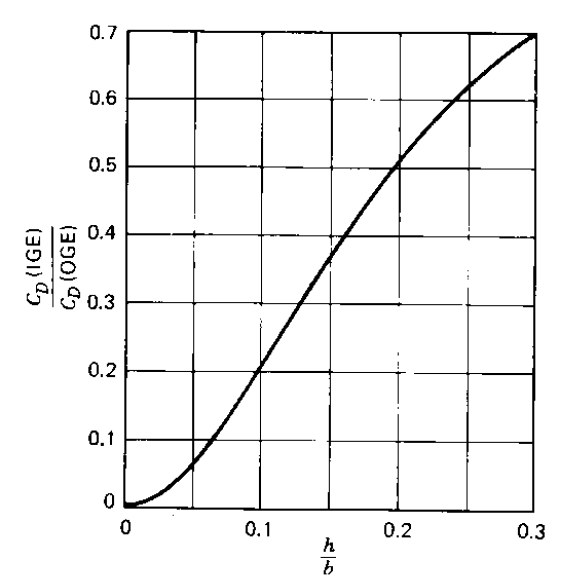
\includegraphics[keepaspectratio, width=0.6\textwidth]{McCormickGroundEffect}
\caption{Gorund effect parameter $K_g$ as function of the $h_{\text{W}}/b$ ratio}
\label{fig:McCormickGroundEffect}
\end{figure}
%
\begin{equation}
K_g=-622.44x^5+624.46x^4-255.24x^3+47.105x^2-0.6378x+0.0055
\label{eqn:FifthOrderPoly}
\end{equation}
%
This polynomial equation has a coefficient of determination $R^2$ of 0.9999 which justifies the approximation.
%
\begin{figure}[!t]
\centering
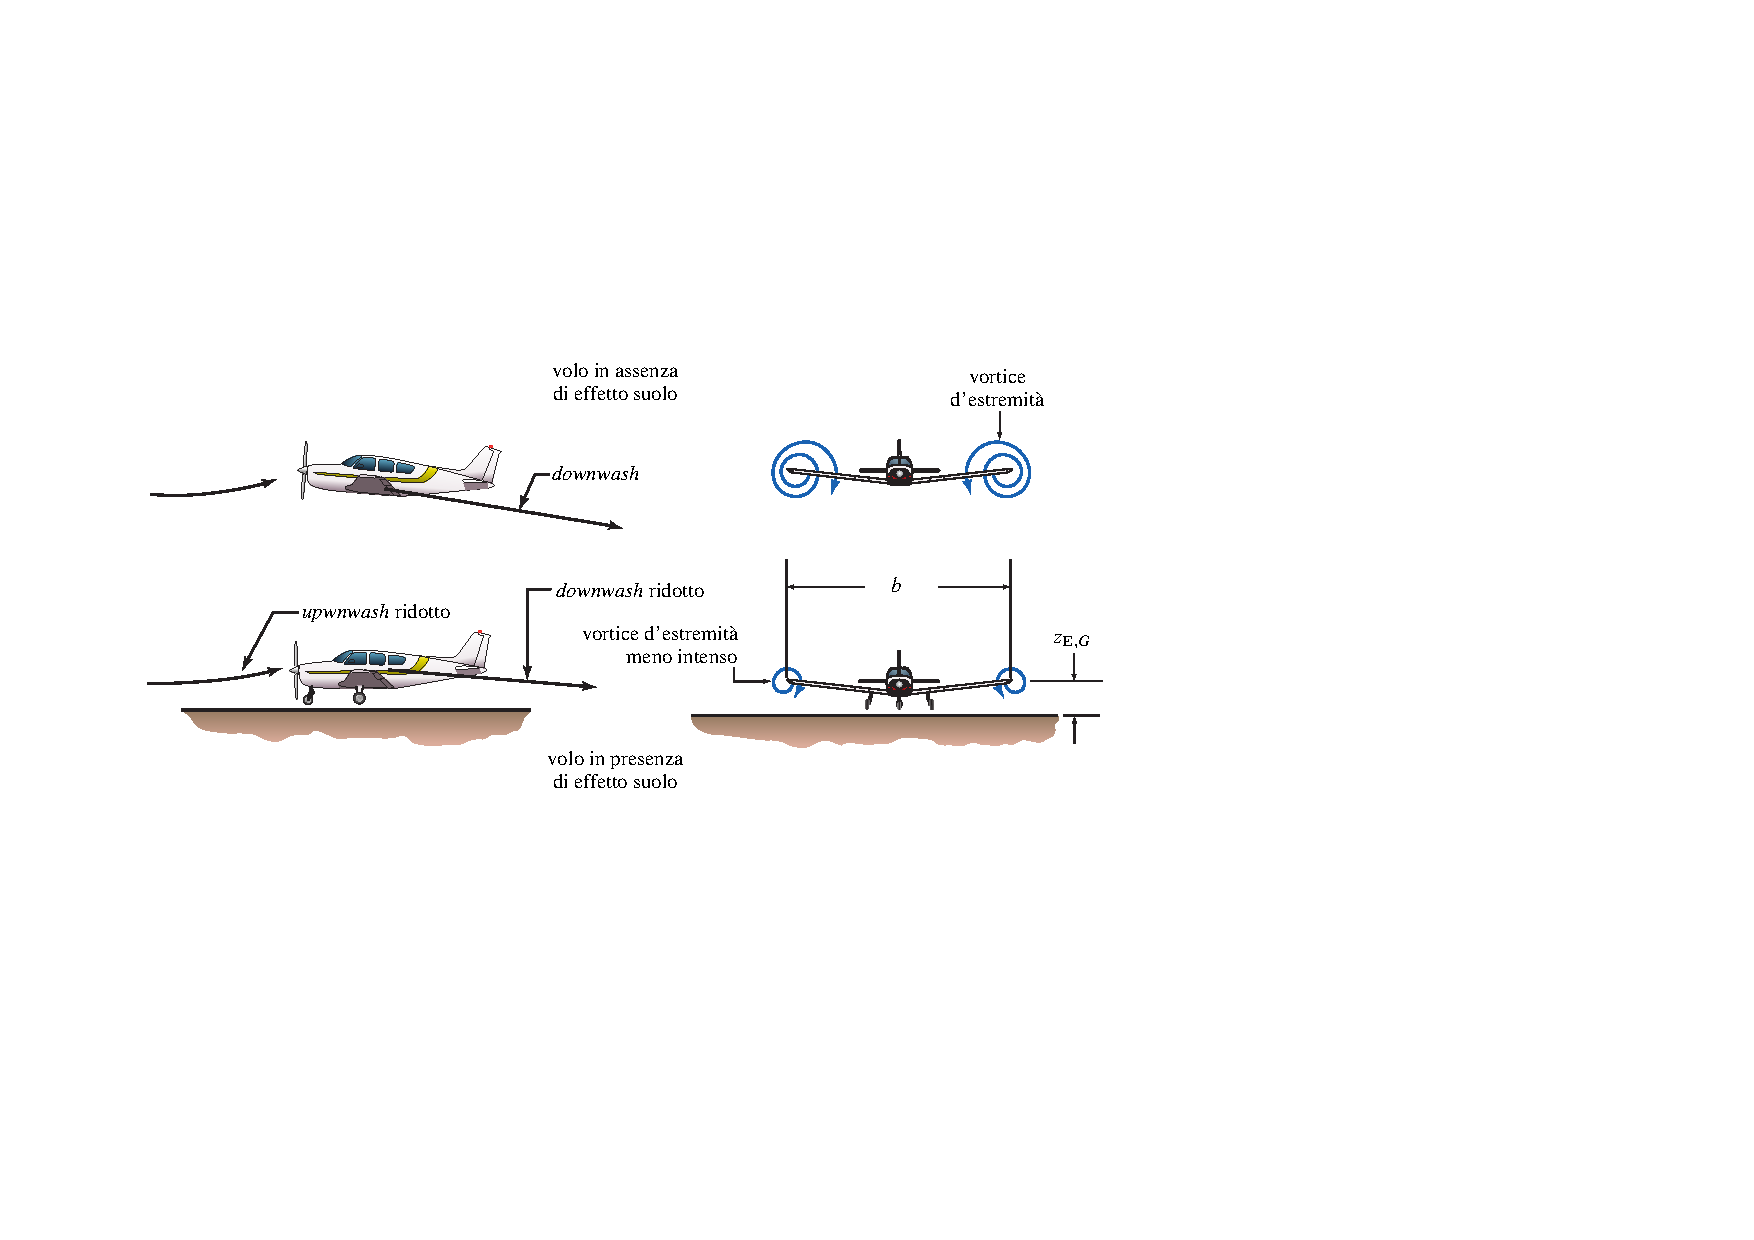
\includegraphics[keepaspectratio, width=\textwidth]{GroundEffect}
\caption{Comparison between flight with and without ground effect}
\label{fig:GroundEffect}
\end{figure}

\bigskip
\noindent
In order to better understand the nature of the ground effect it is convenient to refer to~\cite{nicolai2010fundamentals}, where the ground effect is explained as follows.
%
As the aircraft flies close to the ground, the ground interferes with the horseshoe vortex system trailing behind the wing. Ground effect is often analyzed by putting an image horseshoe vortex system of equal but opposite strength at the same distance $h_{\text{W}}$ below the ground.
%
This image vortex system induces velocities at the wing aerodynamic center, which decreases the strength of the downwash at that point, thereby decreasing the induced angle of attack, $\alpha_i$. Thus, the wing $C_L$ is increased (or more correctly, the lift curve slope increases, giving an increase in $C_L$ for the same geometric angle of attack, $\alpha$) and the induced drag is decreased.
%
This influence of the ground effect is a function of how close the aircraft is to the ground and of the size of the wing.

\bigskip
\noindent
Speaking of the $C_D$, it has also to be noted that, at high $C_L$, the parabolic drag polar it's no longer accurate in describing the drag characteristics of the aircraft so that two correction factors have to be added to the (\ref{eq:CD:A}). These latter triggers only when the $C_L$ is higher than 1.2, as can be seen from the following equation, in which $K_1$ and $K_2$ values depend on the aircraft in exam.
%
\begin{equation}
C_D = C_{D0} + \left(\upDelta C_{D0}\right)_{\text{flap}+\text{lg}} +  K_g\ \frac{C_L^2}{\pi \AR e} + K_1\ \left(C_L-1.2\right) + K_2\ \left(C_L-1.2\right)^2
\end{equation}

\bigskip
\noindent
Focusing, now, on the input law of the angle of attack, the function $u$ can be constructed by picking the time $t_{\text{Rot}}$ when the rotation speed $V_{\text{Rot}}$ is reached along the ground roll; thus the $u (t)$ function can be defined as follows.

\bigskip
\begin{equation}\label{eq:Take:Off:System:Dynamics:Alpha:Law}
u (t) =
    \LEFTRIGHT\lcbrace.{
      \begin{array}{l@{\rule{2em}{0pt}}l} 
        \alpha_{\text{g}}
          & \text{if} \;\, t < t_{\text{Rot}}
        \\[1em]
        \alpha_1(t)
          & \text{if} \;\, t \geq t_{\text{Rot}}
      \end{array}
    }
\end{equation}
%
with a constant $\alpha_{\text{g}}$ during the ground run up to the rotation speed, and a given non-zero law $\alpha_1(t)$ for the post-rotation angle of attack time history. 
%
\begin{figure}[!t]
\centering
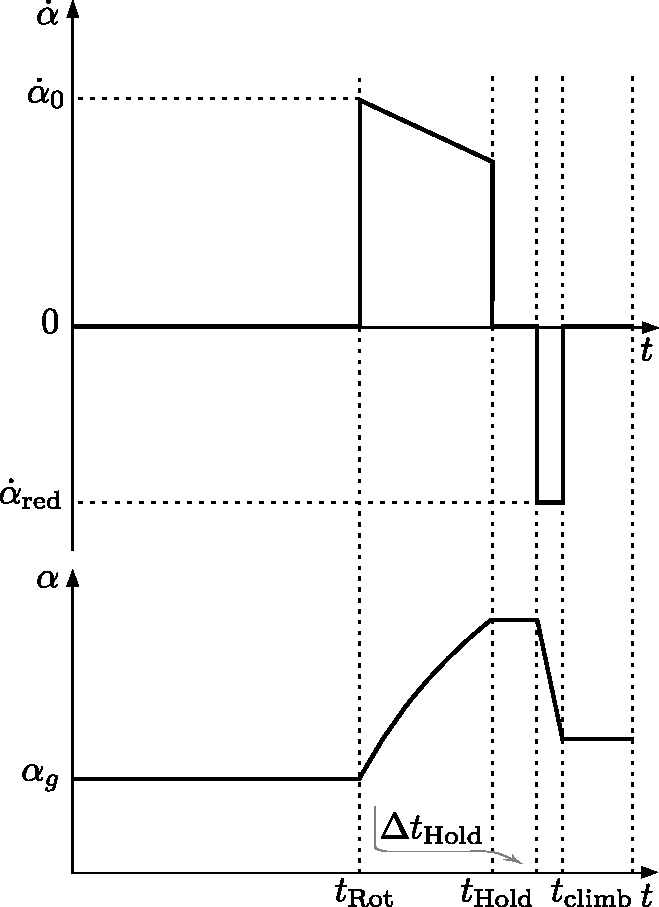
\includegraphics[keepaspectratio, width=0.45\textwidth]{AlphaInputTakeOff}
\caption{Qualitative representation of the angle of attack input law}
\label{fig:AlphaInput}
\end{figure}
%
Figure~\ref{fig:AlphaInput} shows a qualitative representation of the $\alpha_1(t)$ law. As can be seen, after $t_{\text{Rot}}$ the pilot applies an initial angular velocity $\dot\alpha_{0}$, which decreases with time, according to the law written in (\ref{eqn:AlphaDot}) as function of $\alpha$, until the time $t_{\text{Hold}}$ has been reached; this particular instant is related to the achievement of the maximum admitted lift coefficient in take-off, which is set at 90\% of the $C_{L\text{max,TO}}$.
%
\begin{equation}
\dot\alpha=\dot\alpha_0\ \left(1-k_\alpha\ \alpha\right)
\label{eqn:AlphaDot}
\end{equation}
%
\noindent
In equation (\ref{eqn:AlphaDot}), the $k_\alpha$ slope is assigned (expressed in $\si{1/\degree}$ and dependent on the aircraft in exam), while the initial angular velocity $\dot\alpha_0$ is calculated as follows.
%
\begin{equation}
\dot\alpha_0=\dfrac{\upDelta\alpha}{\upDelta t_{\text{Rot}}}=\dfrac{\alpha_{\text{LO}}-\alpha_g}{\upDelta t_{\text{Rot}}}
\label{eqn:AlphaDotInitial}
\end{equation}
%
where $\alpha_{\text{LO}}$ can be obtained from the lift curve of the wing, with flaps deflected in take-off configuration, by assigning the $C_{\text{L}_{\text{LO}}}$; this can be derived from the $C_{L\text{max,TO}}$ dividing it by the parameter $K^2_{\text{LO}}$, which represents the quantity that has to be multiplied by $V_{\text{S}}$ in order to obtain $V_{\text{LO}}$ (for example 1.1 with reference to table~\ref{tab:Take:Off:Speeds:FAR25}).

\bigskip
\noindent
From this point on the pilot stops the pitching manouver and keeps the angle of attack constant for an assigned $\upDelta t_{\text{Hold}}$. During this time interval, the lift coefficient is high and, as a result, also the induced drag is high so that aircraft acceleration will reduce. 
%
After this short time interval the pilot has to reduce the angle of attack in order to avoid the acceleration to decrease too much and so an assigned negative angular velocity $\dot\alpha_{\text{red}}$ is applied; the latter assumed to be constant for simplicity. 
%
Finally, since the decrease of $\alpha$ determines also a reduction in $C_L$, the time $t_{\text{climb}}$ will be reached when the load factor is reduced to 1; this means that a balance of the forces, perpendicular to the flight path, has been achieved and so the climb phase, at constant $\gamma$, can begin, leaving $\alpha$ constant and equal to last value reached. Moreover, from this time on, the lift value is constant and equal to $W\cdot\cos\gamma$, in order to maintain the load factor equal to 1; while the $C_L$ is derived from the lift value using the (\ref{eqn:Lift.Equation}).
%
%-----------------------------OEI Take-Off subsection-----------------------------
\subsection{\gls{acr:OEI} take-off run and balanced field lenght}
\label{subpar:OEI}
A good description of the take-off with one engine failure is proposed in \cite{sforza2014commercial}. Here it is explained that in the event of an engine failure during the take-off roll the pilot must decide whether to continue the take-off or, instead, abort the take-off and decelerate to a stop on the runway. Obviously, if the engine failure occurs when the aircraft is traveling very slowly, the aircraft should be kept on the ground and brought to a stop at some safe location off the runway. Conversely, if the engine failure occurs when the aircraft is close to the take-off speed the take-off should be continued. The designer must provide a means for deciding whether it is safer to abort the take-off or continue it.
%
The critical velocity, denoted as $V_{\text{act}}$, is the velocity at which action is taken, not that at which the decision to act is taken. The time between the recognition of an engine failure, which occurs at $V_{\text{ef}}$, and the critical velocity $V_{\text{act}}$, when action is taken is required to be more than one second. Generally this time period, which is set by the reaction time of the pilot, is taken to be about \SI{3}{\second}. If the pilot’s decision is to continue the take-off with one engine inoperative, the distance to the lift-off speed $V_{\text{LO}}$ and to the subsequent climb-out to 35 $\si{ft}$ height above the runway, will obviously be longer than with all engines operating.

\bigskip
\noindent
The calculation of the take-off distance in this situation is quite the same as the one explained previously, with the difference that now there is a discontinuity in thrust due to the broken engine. In particular, the thrust, $T(x_2)$, will still be read from the database but considering a number of engines reduced by one from the time $t_{\text{ef}}$ at which the engine failure occurs.

\bigskip
\noindent
On the other hand, in the case of the aborted take-off the pilot will apply the necessary braking procedures in order to get the maximum permissible deceleration while maintaining adequate control of the airplane’s motion. The portion of the aborted take-off run up to the engine failure velocity $V_{\text{ef}}$ is calculated in the same way as that for the continued take-off, so that the distance is the same in both cases. 
%
From this point on, until the pilot reacts by activating brakes, there is only a discontinuity in thrust due to the failed engine; while, after the time interval in which the pilot decides to abort the take-off, the thrust is set to minimum (ideally zero) and the brakes action provides an higher friction coefficient. During this last phase, the equation (\ref{eq:Take:Off:System:Dynamics:RHS:functions:B}) changes in the following.
%
\begin{equation}\label{eq:Take:Off:System:Dynamics:RHS:functions:Aborted}
f_2 \big(\, \vec{x}\,,\,u \,\big) =\frac{g}{W}\ \big\{ - D(x_2,u) - \mu_{\text{brakes}} \big[ W - L(x_2,u) \big]\big\} 
\end{equation}
%
where $\mu_{\text{brakes}}$ is bigger than $\mu$ and it is usually about 0.3.
%
Furthermore, it has to be noted that, even if the aircraft in exam is supplied with a reverse thrust device, this effect has not to be taken into account for a more conservative result. 

\bigskip
\noindent
Instead of considering the limiting cases of aborting take-off at low $V_{\text{act}}$ and continued take-off at high $V_{\text{act}}$, it is useful determine the critical velocity for which the distance required to continue the take-off is equal to the distance required to safely abort it. This velocity is the one from table \ref{tab:Take:Off:Speeds:FAR25} and it's called \emph{decision speed} $V_1$, while the related distance is called the \emph{balanced field length}. The latter, in particular, plays an important role in the sizing of the runway since is the maximal distance the aircraft can cover both in continued take-off, both in 
aborted take-off. 
%
In order to calculate this distance, and the related velocity, it's possible to evaluate, at different $V_{\text{act}}$,  both the continued take-off distance with one inoperative engine, both the aborted take-off distance. Each couple of speed and distance can then be plotted with the result of building the curves of figure~\ref{fig:BalancedFieldLength}. The intersection of these latter, at which the two distances are the same, defines the \emph{balanced field length} and the $V_1$.
%
\begin{figure}[H]
\centering
\includegraphics[keepaspectratio, width=0.6\textwidth]{BalancedFieldLength}
\caption{Qualitative representation of the field distances required to continue a takeoff or to abort it when one
engine fails as a function of critical velocity}
\label{fig:BalancedFieldLength}
\end{figure}
%
\noindent
As expected, the take-off distance on the curve related to the continued take-off with one inoperative engine decreases with the failure speed, tending to the AOE condition; while the take-off distance on the other curve grows with the failure speed because the deceleration to stop the aircraft begins from an higher speed, requiring more distance to be dissipated.
%
%------------------------- JAVA CLASS ARCHITECTURE ---------------------------
\section{Java class architecture}
%
In this paragraph the implementation inside the \gls{JPAD} library of the calculation of the take-off distance, and of the related balanced field length, will be desribed; in particular, as in previous chapters, a dedicated Java class, named~\lstinline[language=Java]!CalcTakeOff_Landing!, has been created to manage all required methods.

\bigskip
\noindent
The first component to be described is the class constructor; the latter, in addition to linking all the input parameter to the related class fields, provides a series of preliminary calculations which defines other required input data, not given from the user, such as the maximum lift coefficient in take-off configuration, or the stalling speed in take-off, and some of the characteristic speeds defined in table~\ref{tab:Take:Off:Speeds:FAR25}.
%
\begin{table}[!t]
\makebox[\linewidth]{
\begin{tabular}{p{0.25\linewidth}p{0.7\linewidth}}
\toprule
\lstinline[language=Java]!aircraft! & An \lstinline[language=Java]!Aircraft! class object representing an aircraft parametric model \\ [0.2cm]
\lstinline[language=Java]!theConditons! & An \lstinline[language=Java]!OperatingConditions! object representing aircraft flight conditions \\  [0.2cm]
\lstinline[language=Java]!highLiftCalculator! & A \lstinline[language=Java]!CalcHighLiftDevices! object for managing flap and slat effects \\  [0.2cm]
\lstinline[language=Java]!dtRot! & The assigned time interval of the rotation phase \\  [0.2cm]
\lstinline[language=Java]!dtHold! & The assigned time interval of the constant $C_L$ phase\\  [0.2cm]
\lstinline[language=Java]!kcLMax! & Percentage of the $C_{L\text{max,TO}}$ not to be surpasses \\  [0.2cm]
\lstinline[language=Java]!kRot! & Percentage of $V_s$ which defines the rotation speed \\  [0.2cm]
\lstinline[language=Java]!kLO! & Percentage of $V_s$ which defines the lift-off speed \\  [0.2cm]
\lstinline[language=Java]!kFailure! & A parameter which defines the drag increment due to engine failure and the consequent rudder deflection\\  [0.2cm]
\lstinline[language=Java]!k1! & Linear correction factor of the parabolic drag polar at high $C_L$ \\  [0.2cm]
\lstinline[language=Java]!k2! & Quadratic correction factor of the parabolic drag polar at high $C_L$ \\  [0.2cm]
\lstinline[language=Java]!phi! & Throttle setting \\  [0.2cm]
\lstinline[language=Java]!kAlphaDot! & A coefficient which defines the decrease of $\dot\alpha$ during manouvering \\ [0.2cm]
\lstinline[language=Java]!alphaReductionRate! & A constant negative pitching angular velocity to be maintained after holding the $C_L$ constant \\ [0.2cm]
\lstinline[language=Java]!mu! & The friction coefficient without brakes action \\ [0.2cm]
\lstinline[language=Java]!muBrake! & The friction coefficient with brakes activated \\ [0.2cm]
\lstinline[language=Java]!wingToGroundDistance! & The distance between the wing and the ground  \\ [0.2cm]
\lstinline[language=Java]!obstacle! & A given altitude value to overcome which defines the airborne phase ending \\ [0.2cm]
\lstinline[language=Java]!vWind! & The horizontal component of the wind speed, positive if opposite to the aircraft motion \\ [0.2cm]
\lstinline[language=Java]!alphaGround! & The angle of attack, in the \gls{ACRF}, of the wing when the aircraft is on the ground \\ [0.2cm]
\lstinline[language=Java]!iw! & The angle between the wing root chord and the \gls{ACRF} x-axis \\ 
\bottomrule
\end{tabular}
}
\caption{\lstinline[language=Java]!CalcTakeOff_Landing! constructor input}
\label{table:CalcTakeOffInput}
\end{table}
%
More in detail, the constructor evaluates, firstly, all high-lift devices effects, which data are supplied in the test class as explained in the paragraph~\ref{par:CalcHighLiftDevices}, by using the method~\lstinline[language=Java]!calculateHighLiftDevicesEffects! of the~\lstinline[language=Java]!CalcHighLiftDevices! class, described in the previous chapter in paragraph~\ref{par:CalcHighLiftDevices}. After that it's possible to define the maximum lift coefficient, $C_{L\text{max,TO}}$, the $C_{L0}$, with high-lift devices effects computed, and the lift coefficient during the ground roll phase, $C_{Lg}$, related to the constant angle of attack $\alpha_g$; in particular the last two quantities are calculated using the method~\lstinline[language=Java]!calcCLatAlphaHighLiftDevice!, of the~\lstinline[language=Java]!CalcHighLiftDevices! class, respectively with $\alpha_w=0\degree$ and  $\alpha_w=\alpha_g+i_w$.
%
With the $C_{L\text{max,TO}}$ known, the stalling speed in take-off configuration is calculated using the classical formula provieded below.
%
\begin{equation}
V_s=\sqrt{\dfrac{2W_{\text{TO}}}{\rho\ S\ C_{L\text{max,TO}}}}
\label{eqn:Lift.Equation}
\end{equation} 
%
From this speed, both the $V_{\text{Rot}}$ both the $V_{\text{LO}}$ are calculated multipling the $V_s$ by the two parameters, $k_{\text{Rot}}$ and $k_{\text{LO}}$, defined in table~\ref{table:CalcTakeOffInput}.
%
At this point, the ratio $h_{\text{W}}/b$ and the ground effects correction parameter $K_g$ of the (\ref{eqn:FifthOrderPoly}) are calculated; while all the \gls{List}s, which will store all physical quantities of interest at every integration step, are initialized together with a custom \gls{Map}, named~\lstinline[language=Java]!TakeOffResultsMap!. The latter, in particular, has been created with the purpose of store the state vector, and all the related physical quantities, only at some key point during the take-off run, like the end of the ground roll phase, the end of the rotation phase and the end of the airborne phase.
%
\begin{table}[!t]
\makebox[\linewidth]{
\begin{tabular}{p{0.25\linewidth}p{0.7\linewidth}}
\toprule
\lstinline[language=Java]!timeValue! & The integration time, in $\si{\second}$, at the step to save \\ [0.2cm]
\lstinline[language=Java]!thrustValue! & The engine thrust, in $\si{\newton}$, at the step to save \\  [0.2cm]
\lstinline[language=Java]!thrustHorizontalValue! & The engine thrust component on the \gls{ACRF} x-axis, in  $\si{\newton}$, at the step to save \\  [0.2cm]
\lstinline[language=Java]!thrustVerticalValue! & The engine thrust component on the \gls{ACRF} z-axis, in  $\si{\newton}$, at the step to save \\  [0.2cm]
\lstinline[language=Java]!frictionValue! & The friction, in  $\si{\newton}$, at the step to save\\  [0.2cm]
\lstinline[language=Java]!liftValue! & The lift, in  $\si{\newton}$, at the step to save \\  [0.2cm]
\lstinline[language=Java]!dragValue! & The drag, in  $\si{\newton}$, at the step to save \\  [0.2cm]
\lstinline[language=Java]!totalForceValue! & The total force, in brakets in the equation (\ref{eq:Take:Off:System:Dynamics:RHS:functions:B}), at the step to save in  $\si{\newton}$ \\  [0.2cm]
\lstinline[language=Java]!loadFactorValue! & The load factor at the step to save \\  [0.2cm]
\lstinline[language=Java]!speedValue! & The speed, in  $\si{\meter\per\second}$, at the step to save \\  [0.2cm]
\lstinline[language=Java]!rateOfClimbValue! & The rate of climb from equation (\ref{eq:Take:Off:System:Dynamics:RHS:functions:D}), in  $\si{\meter\per\second}$, at the step to save \\  [0.2cm]
\lstinline[language=Java]!accelerationValue! & The acceleration from equation (\ref{eq:Take:Off:System:Dynamics:RHS:functions:B}), in  $\si{\meter\per\square\second}$, at the step to save \\  [0.2cm]
\lstinline[language=Java]!groundDistanceValue! & The horizontal distance, in  $\si{\meter}$, covered at the step to save \\ [0.2cm]
\lstinline[language=Java]!verticalDistanceValue! & The altitude, in  $\si{\meter}$, reached at the step to save \\ [0.2cm]
\lstinline[language=Java]!alphaValue! & The angle of attack $\alpha$, in  $\si{\degree}$, at the step to save, in \gls{ACRF} \\ [0.2cm]
\lstinline[language=Java]!alphaDotValue! & The pitching angular velocity, in  $\si{\degree\per\second}$, at the step to save \\ [0.2cm]
\lstinline[language=Java]!gammaValue! & The ramp angle $\gamma$, in  $\si{\degree}$, at the step to save  \\ [0.2cm]
\lstinline[language=Java]!gammaDotValue! & The $\dot\gamma$ value, in  $\si{\degree\per\second}$, at the step to save \\ [0.2cm]
\lstinline[language=Java]!thetaValue! & The $\theta=\alpha+\gamma$ value, in  $\si{\degree}$, at the step to save \\ [0.2cm]
\lstinline[language=Java]!cLValue! & The lift coefficient at the step to save \\ [0.2cm]
\lstinline[language=Java]!cDValue! & The drag coefficient at the step to save \\ 
\bottomrule
\end{tabular}
}
\caption{\lstinline[language=Java]!collectResults! input data}
\label{table:TakeOffMapInput}
\end{table}

\bigskip
\noindent
The~\lstinline[language=Java]!TakeOffResultsMap! class is made up of a builder, which accepts nothing as input and provides the initialization of all the \gls{List}s required to store the wanted data, and of other two method which are explained below.
%
\begin{itemize}
\item \lstinline[language=Java]!initialize!, which clears all the \gls{List}s in order to make them reusable for other calculations
\item \lstinline[language=Java]!collectResults!, which accepts as input all data from table~\ref{table:TakeOffMapInput} in order to add them to the related \gls{List}
\end{itemize}
%
Once all data are stored, it's easy with this \gls{Map} to get one, or more than one, result; all it has to be done is call the related \emph{getter} method of which the class is supplied. 

\bigskip
\noindent
It has to be noted that all these preliminary calculations and \gls{List}s initializations are put into the constructor for a reason; in fact, as these are all quite heavy operations in terms of computational cost, put them in the constructor means that they are carried out only once allowing a more rapid use, even iterative, of the main method that will be described shortly.

\bigskip
\noindent
The most important method of the class is~\lstinline[language=Java]!calculateTakeOffDistanceODE! which is in charge of the resolution of the \gls{acr:ODE} set presented in (\ref{eq:Take:Off:System:Dynamics:RHS:functions}). This method accepts as input two parameters which are used to determine, firstly, if an engine failure has occurred during the take-off run, and then if the take-off run has to be aborted; these are:
%
\begin{itemize}
\item \lstinline[language=Java]!vFailure!, a \lstinline[language=Java]!Double! value representing the failure speed in $\si{\meter\per\second}$. Can be set to \lstinline[language=Java]!null! if the user dosen't want to calculate the \gls{acr:OEI} take-off distance. 
\item \lstinline[language=Java]!isAborted!, a \lstinline[language=Java]!boolean! flag which is \lstinline[language=Java]!true! if the method has to calculate the aborted take-off distance.
\end{itemize}
%
After performing a check upon these two variables, the method knows which case it has to study and proceeds with the calculation; in particular, it creates the integrator object of the class \lstinline[language=Java]!HighamHall54Integrator!, which implements the \gls{Interface} \lstinline[language=Java]!FirstOrderIntegrator!. For more information, the reader can refer to \cite{apache:ode}.

\bigskip
\noindent
More in detail, the \lstinline[language=Java]!HighamHall54Integrator! class implements a fifth order Higham and Hall integrator which uses seven functions evaluations per step and is supplied with stepsize control, automatic step initialization and continuous output. The latter has proven to be the best choise, among other possible integrators (viewables in \cite{apache:FirstOrderIntegrator}) which implement the previous \gls{Interface}, because it provides the better compromise between calculation time and accuracy using the following settings.

\bigskip
\begin{lstlisting}[caption={HighamHall54Integrator class object creation}, captionpos=b, tabsize=2]
FirstOrderIntegrator theIntegrator = new HighamHall54Integrator(
				1e-6,				// minimal step 
				1,				  // maximal step 
				1e-17,			// allowed absolute error
				1e-17				// allowed relative error
				);
\end{lstlisting}
%
Beside the integrator, the method needs the set of equation to integrate; these are passed to it through the object of a dedicated inner class, named \lstinline[language=Java]!DynamicsEquations!, which implements the \gls{Interface} \lstinline[language=Java]!FirstOrderDifferentialEquations! \cite{apache:FirstOrderDifferentialEquations}. Thus, the \lstinline[language=Java]!DynamicsEquations! class provides the set of \gls{acr:ODE} (\ref{eq:Take:Off:System:Dynamics:RHS:functions}) and, in particular, is supplied with a series of methods necessary to calculate the required physical quantities used into these equations and described in the previous paragraph. Furthermore, thanks to the use of the variable \lstinline[language=Java]!isAborted!, the class can easly switch the equations set in case of aborted take-off as shown in the subparagraph \ref{subpar:OEI}.
%
\begin{table}[!b]
\begin{tabular}{p{0.17\linewidth}p{0.83\linewidth}}
\toprule
\lstinline[language=Java]!ehCheckFailure! & It checks when the speed, $x_2$, becomes greater than the input \lstinline[language=Java]!vFailure! determining, in this way, the instant of the engine failure occurrence \\ [0.2cm]
\lstinline[language=Java]!ehCheckVRot! & It checks when the speed, $x_2$, becomes greater than the rotation speed \lstinline[language=Java]!vRot! determining, in this way, the instant at which the ground roll ends and the rotation phase begins \\  [0.2cm]
\lstinline[language=Java]!ehEndConstantCL! & It checks when the time, $t$, becomes greater than the sum of  $t_{\text{Hold}}$ and of the given time interval $\upDelta t_{\text{Hold}}$ determining, in this way, the instant at which the angle of attack, and the related $C_L$, stops to be kept constant \\  [0.2cm]
\lstinline[language=Java]!ehCheckObstacle! & It checks when the altitude, $x_4$, becomes greater than the given obstacle height (35 $\si{ft}$) determining, in this way, the instant at which the airborne phase, and so the entire take-off, ends \\  [0.2cm]
\lstinline[language=Java]!ehCheckBrakes! & It checks when the time, $t$, becomes greater than the sum of  $t_{\text{Failure}}$ and of the given time interval $\upDelta t_{\text{Rec}}$, required to the pilot to recognize the failure, determining, in this way, the instant at which the pilot, which has decided to abort the take-off, actions the brakes in order to stop the aircraft run\\  [0.2cm]
\lstinline[language=Java]!ehCheckStop! &  It checks when the speed, $x_2$, becomes lower than zero determining, in this way, the instant at which the aircraft has stopped \\ 
\bottomrule
\end{tabular}
\caption{\lstinline[language=Java]!EventHandler! implementation inside the method \lstinline[language=Java]!calculateTakeOffDistanceODE!}
\label{table:EventHandler}
\end{table}

\bigskip
\noindent
In order to take into account of particular events which can happen during the take-off run, the method \lstinline[language=Java]!calculateTakeOffDistanceODE! is supplied with several implementation of the \gls{Interface} \lstinline[language=Java]!EventHandler! \cite{apache:ode}. The latter, through the definition of a specific function, can determine the occurrence of the wanted event by monitoring whether the sign of the defined function changes. Moreover it allows to manage the time step at which the event has occurred, so that it's possible to save, into the~\lstinline[language=Java]!TakeOffResultsMap!, the state vector and all the physical quantities of interest. Each implementation of the \gls{Interface} can also impose one of the folllowing actions to the integrator.
%
\begin{itemize}
\item \textbf{CONTINUE}, the integration simply goes on
\item \textbf{STOP}, the integration stops when the event triggers
\item \textbf{RESET_STATE}, the state vector can be changed when the event triggers 
\item \textbf{RESET_DERVATIVES}, the set of equation can be changed when the event triggers 
\end{itemize}
%
In the case in exam, six events are monitored by six implementation of the \lstinline[language=Java]!EventHandler! \gls{Interface} as shown below.

\noindent
Each event of the table \ref{table:EventHandler} defines a time instant usable, by the class \lstinline[language=Java]!DynamicsEquations!, to determine when the derivatives, or the calculation of the related physical quantities, have to switch from an equation to another, this allows to manage in a very easy way the definition of the profile of $\dot\alpha$ and $\alpha$, as well as the derivatives change shown in (\ref{eq:Take:Off:System:Dynamics:RHS:functions:B}) and (\ref{eq:Take:Off:System:Dynamics:RHS:functions:C}).  

\bigskip
\noindent
In order to make each \lstinline[language=Java]!EventHandler! usable by the integrator, they have to be added to the \lstinline[language=Java]!HighamHall54Integrator! as follows.

\bigskip
\begin{lstlisting}[caption={HighamHall54Integrator class object creation}, captionpos=b, tabsize=2]
if(!isAborted) {
	theIntegrator.addEventHandler(ehCheckVRot, 1.0, 1e-3, 20);
	theIntegrator.addEventHandler(ehCheckFailure, 1.0, 1e-3, 20);
	theIntegrator.addEventHandler(ehEndConstantCL, 1.0, 1e-3, 20);
	theIntegrator.addEventHandler(ehCheckObstacle, 1.0, 1e-3, 20);
}
else {
	theIntegrator.addEventHandler(ehCheckVRot, 1.0, 1e-3, 20);
	theIntegrator.addEventHandler(ehCheckFailure, 1.0, 1e-3, 20);
	theIntegrator.addEventHandler(ehCheckBrakes, 1.0, 1e-3, 20);
	theIntegrator.addEventHandler(ehCheckStop, 1.0, 1e-6, 20);
}
\end{lstlisting}
%
As can be seen the \lstinline[language=Java]!boolean! variable \lstinline[language=Java]!isAborted! plays an important role in determining which events have to be checked whether or not the take-off is aborted or continued. Also noteworthy, the method \lstinline[language=Java]!addEventHandler! arguments, which represent, respectively, the following parameters.
%
\begin{itemize}
\item The event to be checked
\item The maximal time interval between switching function checks (this interval prevents missing sign changes in case the integration steps becomes very large)
\item The convergence threshold in the event time search
\item The upper limit of the iteration count in the event time search
\end{itemize}
%
The decision of these parameters values has derived from a compromise between accuracy and computational time.

\bigskip
\noindent
Another important feature that the \gls{acr:ODE} package provides is the possibility to manage each time step, even if no event is triggered; in this way the developer can, for example, store data into an output file, or manage some events which are independent from the time or the state vector as they were in the \lstinline[language=Java]!EventHandler! \gls{Interface}. The tool which allows all these feature is the \lstinline[language=Java]!StepHandler! \gls{Interface} \cite{apache:ode}; in this particular case, this \gls{Interface} has only one implementation, added to the integrator, which is in charge of store the state vector, the time and all the related physical quantities, into their related \gls{List}s, at every time step in order to make them usable outside this method. Moreover it has a key role in managing three events, to be observed only if the variable \lstinline[language=Java]!isAborted! is false, that could not be handled well by the \lstinline[language=Java]!EventHandler! \gls{Interface}; these are the followings.
%
\begin{itemize}
\item A check upon the load factor to catch the instant at which, for the first time, it reaches a value of 1; this instant is $t_{\text{EndRot}}$ and determines the beginning of the airborne phase together with the changes in the derivatives shown in (\ref{eq:Take:Off:System:Dynamics:RHS:functions:B}) and (\ref{eq:Take:Off:System:Dynamics:RHS:functions:C})
\item A check upon the $C_L$ in order to determine when it reaches the threshold value defined by \lstinline[language=Java]!kcLMax! multiplied for the $C_{L\text{max,TO}}$. The related instant is the $t_{\text{Hold}}$ of the beginning of the constant $\alpha$ and $C_L$ phase
\item A second check on the load factor in order to define the instant at which its value is reduced to 1 after having applied the constant $\dot\alpha_{\text{Red}}$ angular velocity. This instant defines~$t_{\text{climb}}$ 
\end{itemize}
%
Each of these events is monitored by the value of the variable \lstinline[language=Java]!isAborted! and by the observation both of the evolution, through a single time step, of the last value added to the \gls{List} of interest, both of the time, which is compared to one of the reference instants described previously.

\bigskip
\noindent
The method is, finally, completed by assigning the initial state vector, calling the method \lstinline[language=Java]!integrate!, which is in charge of the integration process, and ereasing all the \lstinline[language=Java]!StepHandler! and \lstinline[language=Java]!EventHandler! implementations at the end of the process; this in order to make the method reusable later.

\bigskip
\noindent
Now that a method for calculating the take-off distance, in every case, is available, it can be used iteratively in order to determine the \emph{balanced field length} and the related \emph{decision speed} $V_1$. The method in charge of this is called \lstinline[language=Java]!calculateBalancedFieldLength! and follows the following guideline.
%
First of all an array of five values of possible failure speeds (between 2~$\si{\meter\per\second}$ and the lift-off speed $V_{\text{LO}}$) is defined; after that the method \lstinline[language=Java]!calculateTakeOffDistanceODE! is called for each of these speeds both in case of \gls{acr:OEI} continued take-off (\lstinline[language=Java]!isAborted! set to \lstinline[language=Java]!false!), both in case of aborted take-off (\lstinline[language=Java]!isAborted! set to \lstinline[language=Java]!true!). It's important to highlight that between each call of the method \lstinline[language=Java]!calculateTakeOffDistanceODE!, all reference instants and \gls{List}s have to be reinitialized; this can be done using the dedicated method \lstinline[language=Java]!initialize! defined into this class.

\bigskip
\noindent
Each failure speed, \gls{acr:OEI} take-off distance and aborted take-off distance calculated this way, is then stored into a dedicated array so that it's possible to define an interpolating function for the two distances. More in detail, since five points are few to describe the curves in figure \ref{fig:BalancedFieldLength}, a new array of 250 values of failure speeds is defined useing the same constrain of the previous one; the latter is then used to build a spline interpolating function, for both the \gls{acr:OEI} take-off distance and aborted take-off distance, using the five points calculated previously.
%
From the intersection of the last two interpolated curves is possible to define the \emph{balanced field length} and the \emph{decision speed} $V_1$ as shown in figure \ref{fig:BalancedFieldLength}. It should be noted that the choise of using interpolating functions and not to perform more times the calculation of the take-off distance in the two cases, derives from the will to speed up the calculation so that it's possible to have accurate results in less than one second. 

\bigskip
\noindent
In conclusion, the class is completed by two methods in charge of plotting the curves of interst from the related \gls{List}s and the \emph{balanced field length} chart; these are the followings.
%
\begin{itemize}
\item \lstinline[language=Java]!createTakeOffCharts!, provides the conversion of the previous \gls{List}s into \lstinline[language=Java]!double! arrays so that they can be managed by the plotting method; morever it uses the varaible \lstinline[language=Java]!isAborted! to determine which charts have to be plotted since some of them are useless in case of the aborted take-off
\item \lstinline[language=Java]!createBalancedFieldLengthChart!, provides the creation of the chart of figure \ref{fig:BalancedFieldLength} using the interpolated curves, on the y-axis, and the speed array with 250 values, on the x-axis 
\end{itemize}
%
\begin{figure}[H]
\centering
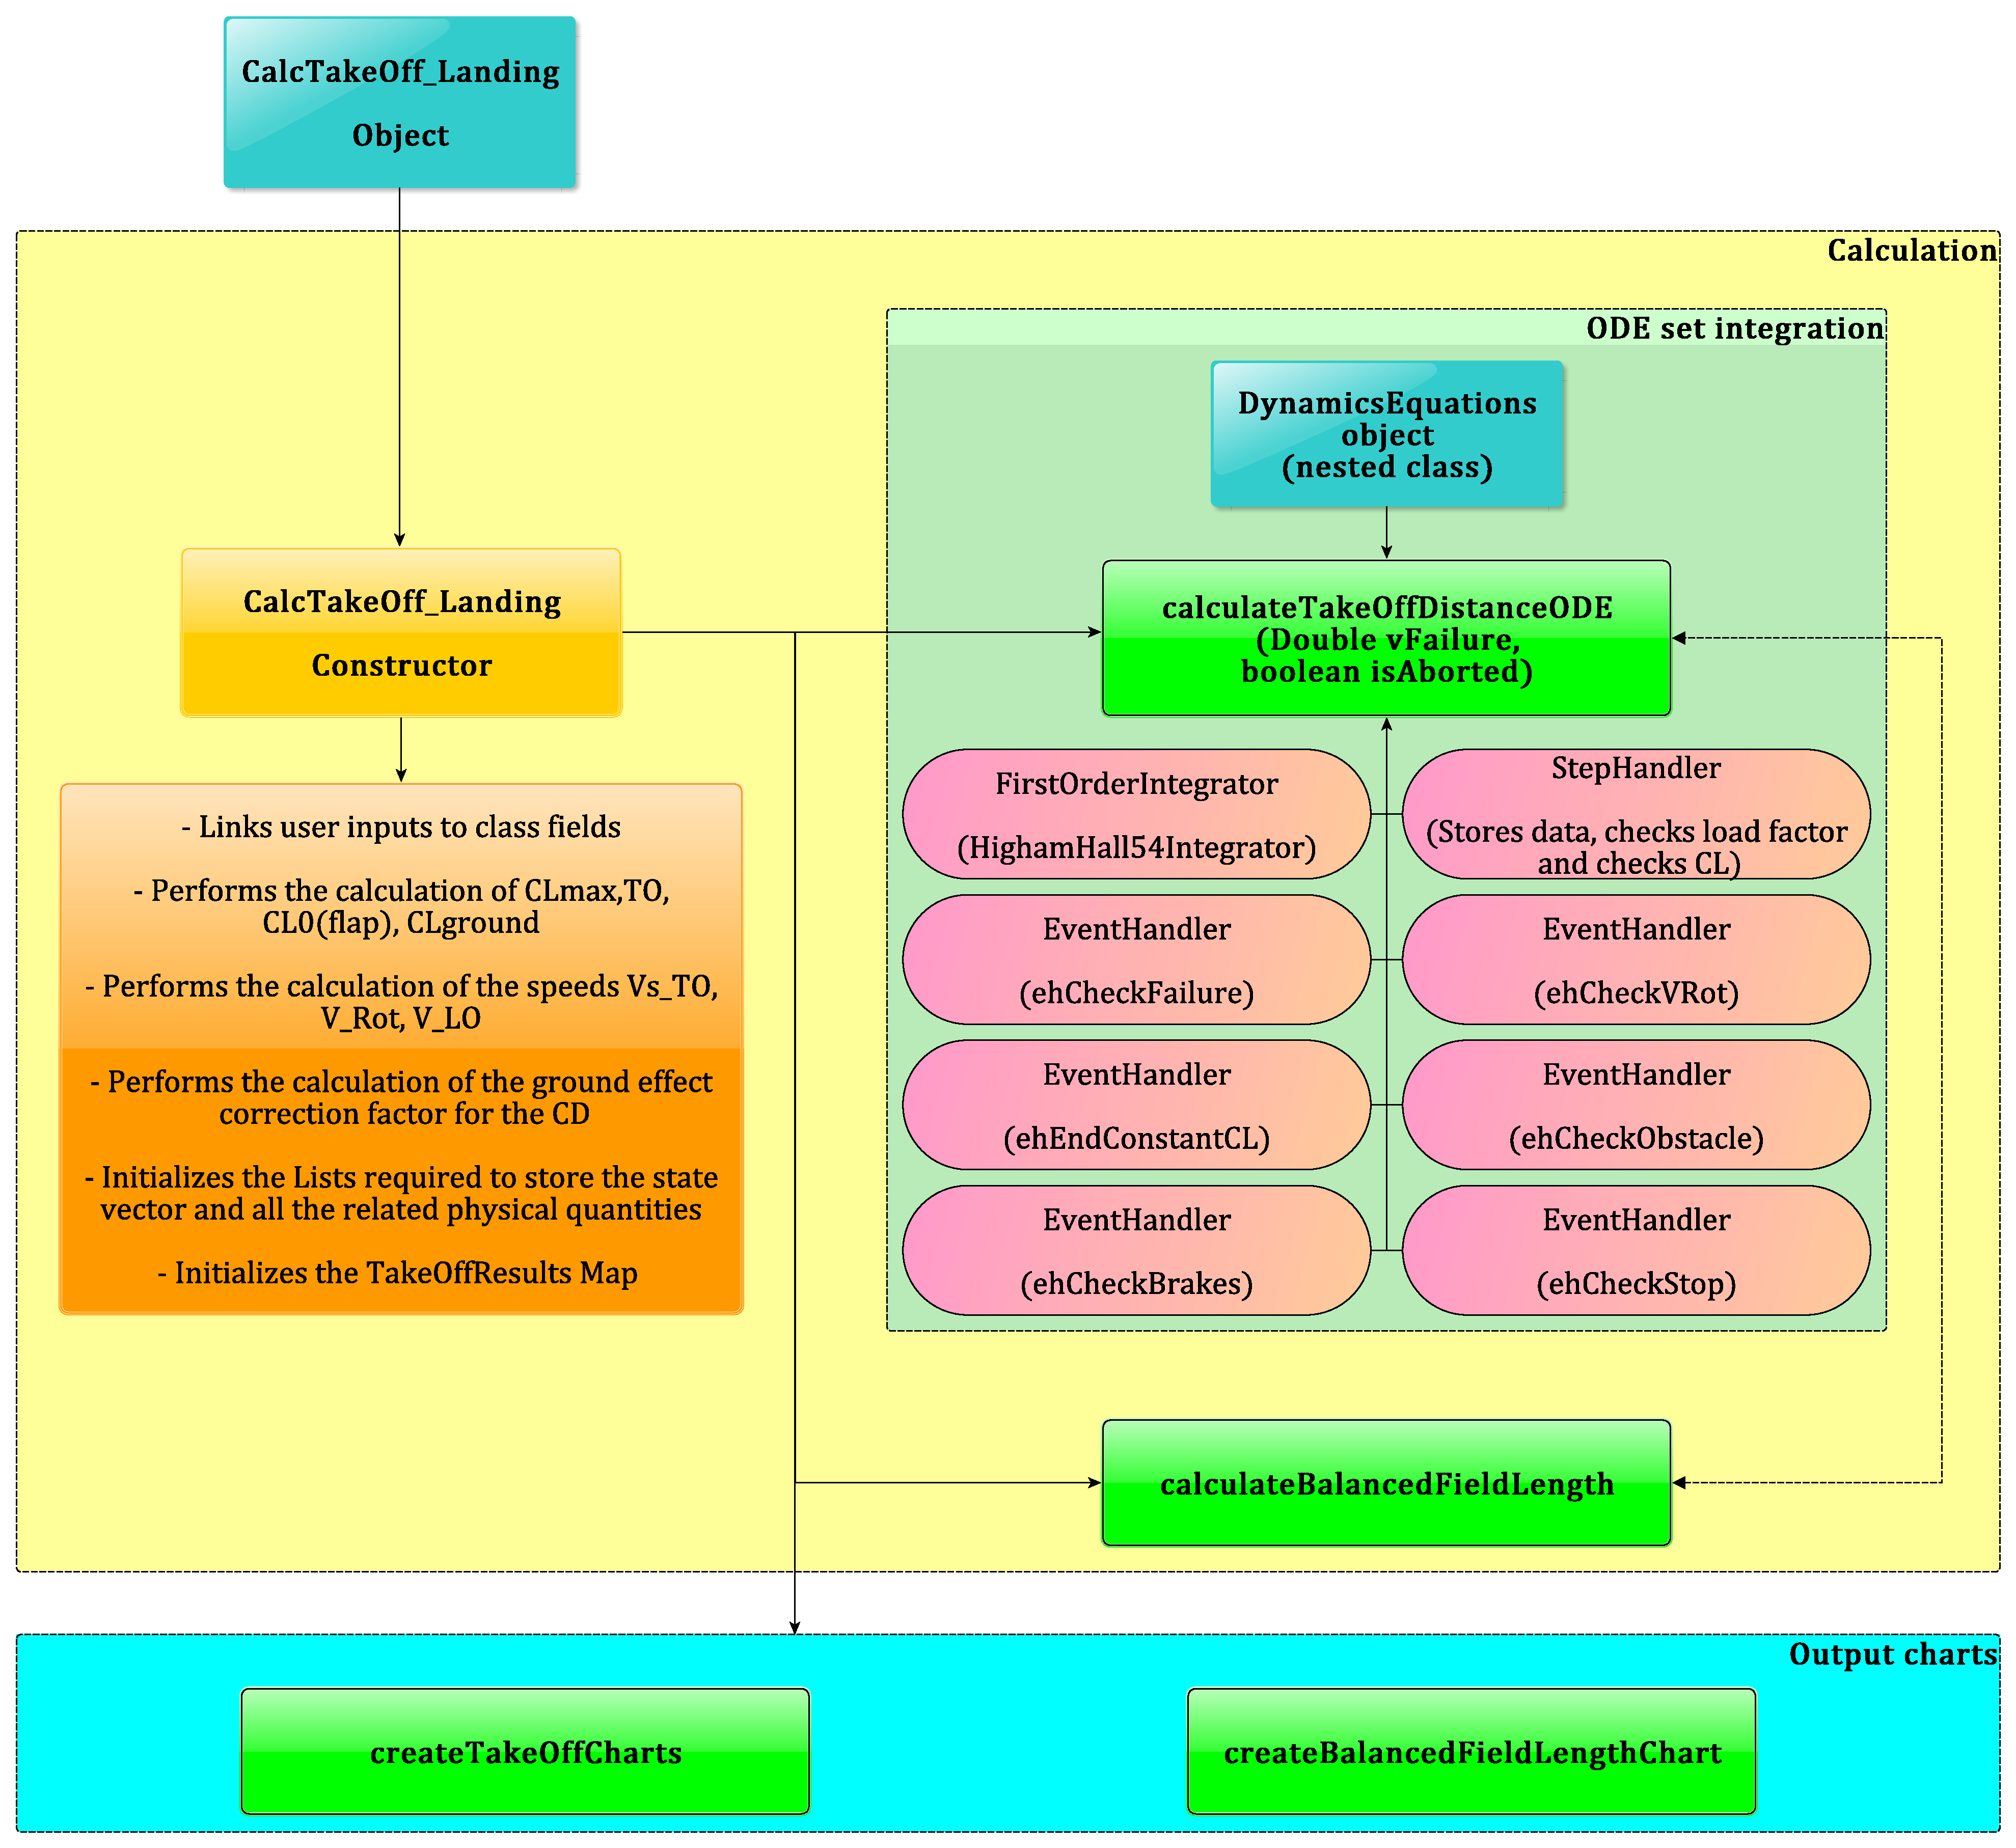
\includegraphics[keepaspectratio, width=\textwidth]{TakeOff_Flowchart}
\caption{\lstinline[language=Java]!CalcTakeOff_Landing! class flowchart}
\label{fig:CalcTakeOffFlowchart}
\end{figure}
%
%----------------------- CASE STUDY : ATR72 AND B747 -------------------------
\section{Case study: ATR-72}
This conclusive paragraph has the aim of describing the Java class created to test the features implemented into \lstinline[language=Java]!CalcTakeOff_Landing! class; in particular a description of how to build the class will be provided in order to help a potential \gls{User:Developer} as well as the presentation and the comment of the most important charts created with the purpose of validating the results obtained. 
%
Since the calculations are the same both for the B747-100B, both for the ATR-72, only the latter will be analyzed. 

\noindent
The first thing to do is to build the aircraft parametric model, and its analysis object, as described in paragraph \ref{par:DefaultAircraft}; then all information regarding high-lift devices have to be provided, in the same way of paragraph \ref{par:CaseStudyHighLift}, in order to allow the constructor of \lstinline[language=Java]!CalcTakeOff_Landing! class to evaluate their effects. 
%
At this point all the preliminary steps are completed and it's possible to create the \lstinline[language=Java]!CalcTakeOff_Landing! object giving as input all data from table \ref{table:CalcTakeOffInput}.

\bigskip
\begin{lstlisting}[caption={Input data and \lstinline!CalcTakeOff_Landing! object creation }, captionpos=b, tabsize=2]
		Amount<Duration> dtRot = Amount.valueOf(3, SI.SECOND);
		Amount<Duration> dtHold = Amount.valueOf(0.5, SI.SECOND);
		double mu = 0.025;
		double muBrake = 0.3;
		double kAlphaDot = 0.06; // [1/deg]
		double kcLMax = 0.85;
		double kRot = 1.05;
		double kLO = 1.1;
		double kFailure = 1.1;
		double phi = 1.0;
		double alphaReductionRate = -3; // [deg/s]
		Amount<Length> wingToGroundDistance = Amount.valueOf(4.0, SI.METER);
		Amount<Length> obstacle = Amount.valueOf(35, NonSI.FOOT).to(SI.METER);
		Amount<Velocity> vWind = Amount.valueOf(0.0, SI.METERS_PER_SECOND);
		Amount<Angle> alphaGround = Amount.valueOf(0.0, NonSI.DEGREE_ANGLE);
		Amount<Angle> iw = Amount.valueOf(2.0, NonSI.DEGREE_ANGLE);
//		PARAMETERS USED TO CONSIDER THE PARABOLIC DRAG POLAR CORRECTION AT HIGH CL
		double k1 = 0.0;
		double k2 = 0.0;
	
		CalcTakeOff_Landing theTakeOffLandingCalculator = new CalcTakeOff_Landing(
				aircraft,
				theCondition,
				highLiftCalculator,
				dtRot,
				dtHold,
				kcLMax,
				kRot,
				kLO,
				kFailure,
				k1,
				k2,
				phi,
				kAlphaDot,
				alphaReductionRate,
				mu,
				muBrake,
				wingToGroundDistance,
				obstacle,
				vWind,
				alphaGround,
				iw
				);
\end{lstlisting}
%
Now if the user wants to perform a single calculation of the take-off distance, he can call the method \lstinline[language=Java]!calculateTakeOffDistanceODE!, specifing the condition he wants to analyze. The possible situations are resumed below, where \lstinline[language=Java]!vFailure! is an assigned \lstinline[language=Java]!Double! value.

\bigskip
\begin{lstlisting}[caption={Possible scenarios of calculation of the take-off distance}, captionpos=b, tabsize=2, label={lst:TakeOffScenarios}]
// AOE condition
theTakeOffLandingCalculator.calculateTakeOffDistanceODE(null, false); 
// OEI continued take-off
theTakeOffLandingCalculator.calculateTakeOffDistanceODE(vFailure, false); 
// OEI aborted take-off
theTakeOffLandingCalculator.calculateTakeOffDistanceODE(vFailure, true); 
\end{lstlisting}
%
Since this method provides only calculations, the user may want to generate charts regarding the evolution of the state vector and of the related physical quantities during the take-off run; in this case all it has to be done is call the method \lstinline[language=Java]!createTakeOffCharts! as shown below.

\bigskip
\begin{lstlisting}[caption={Take-off charts creation}, captionpos=b, tabsize=2]
// Generates all the output charts
theTakeOffLandingCalculator.createTakeOffCharts();
\end{lstlisting}
%
Following the flowchart of figure \ref{fig:CalcTakeOffFlowchart}, if the user wants, instead, to calculate the \emph{balanced field length}, and plot its chart, it's still very easy; in fact he has only to call the two methods \lstinline[language=Java]!calculateBalancedFieldLength! and \lstinline[language=Java]!createBalancedFieldLengthChart!.

\bigskip
\begin{lstlisting}[caption={Balanced field length calculation and plot}, captionpos=b, tabsize=2]
// Calculation of the balanced field length
theTakeOffLandingCalculator.calculateBalancedFieldLength();
// Plot of the balanced field length chart
theTakeOffLandingCalculator.createBalancedFieldLengthChart();
\end{lstlisting}
%
The following pages shows a summary of charts created in the three condition of listing \ref{lst:TakeOffScenarios} choosing a \lstinline[language=Java]!vFailure! of 30 $\si{\meter\per\second}$. Instead, in the listing below, are resumed the main result of the \gls{acr:AOE} condition together with the results of the \emph{balanced field length} calculation.

\bigskip
\begin{lstlisting}[caption={ATR-72 test results}, captionpos=b, tabsize=2]
CLmaxTO = 2.0212498531249747
VsTO = 54.7262494000153 m/s
VRot = 57.4625618700161 m/s
vLO = 60.1988743400169 m/s
CL0 = 1.0741952614143324
CLground = 1.2573301946144486
-----------------------------------------------------------------
		END OF GROUND ROLL PHASE
	switching function changes sign at t = 25.798463352896295 s
	x[0] = s = 805.6857140622815 m
	x[1] = V = 57.4625618700161 m/s
	x[2] = gamma = 0.0 deg
	x[3] = altitude = 0.0 m
	COLLECTING DATA AT THE END OF GROUND ROLL PHASE ...
---------------------------DONE!-------------------------------
		END OF ROTATION PHASE
	x[0] = s = 969.8307390403536 m
	x[1] = V = 61.80076798783429 m/s
	x[2] = gamma = 0.0 deg
	x[3] = altitude = 0.0 m
	t = 28.550529077966075 s
	COLLECTING DATA AT THE END OF ROTATION PHASE ...
---------------------------DONE!-------------------------------
		BEGIN BAR HOLDING
	CL = 1.718569601482539
	Alpha Body = 5.037672106777929 deg
	t = 29.788098164419022 s
---------------------------DONE!-------------------------------
		END BAR HOLDING
	switching function changes sign at t = 30.28809816441902 s 
---------------------------DONE!-------------------------------
		LOAD FACTOR = 1 IN CLIMB
	t = 31.38918339811157 s
---------------------------DONE!-------------------------------
		END OF AIRBORNE PHASE
	switching function changes sign at t = 33.374058565110616 s
	x[0] = s = 1281.9765437949968 m
	x[1] = V = 67.04253409907443 m/s
	x[2] = gamma = 2.8305305752769097 deg
	x[3] = altitude = 10.668000000000013 m
	COLLECTING DATA AT THE END OF AIRBORNE PHASE ...
---------------------------DONE!-------------------------------
BALANCED FIELD LENGTH = 1844.57965640814 m
Decision Speed (V1/VsTO) = 1.04020737941333 
---------------------------END!!-------------------------------
\end{lstlisting}
%
As can be seen the take-off distance required in \gls{acr:AOE} condition is about $\SI{1282}{\meter}$, at the maximum take-off weight of $\SI{23063.579}{\kilogram}$, within a time of about $\SI{33.4}{\second}$; while the \emph{balanced field lenght} is bigger than the AOE take-off distance of about the 30\%.  Moreover the \emph{decision speed} $V_1$ is bigger than the stalling speed $V_s$ and lower than the rotation speed $V_{\text{Rot}}$ as required by the \gls{FAR}-25 from table \ref{tab:Take:Off:Speeds:FAR25}.
%
These results are almost the same shown in the aircraft brochure available on the Internet, so that the calculation carried out results correct.
%
\clearpage
%
\begin{figure}[H]
\centering
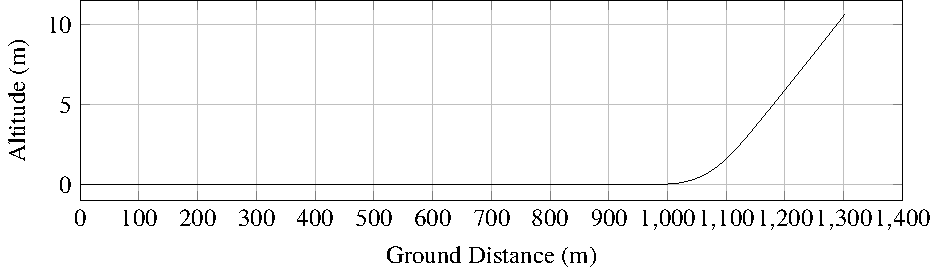
\includegraphics[keepaspectratio, width=1.1\textwidth]{TakeOff_Trajectory_AOE}
\caption{Take-off trajectory in AOE condition - ATR-72}
\end{figure}
%
\begin{figure}[H]
\centering
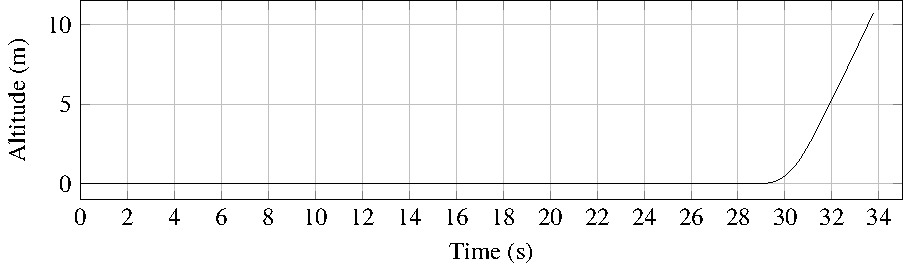
\includegraphics[keepaspectratio, width=1.1\textwidth]{Altitude_evolution_AOE}
\caption{Altitude evolution in AOE condition - ATR-72}
\end{figure}
%
\begin{figure}[H]
\centering
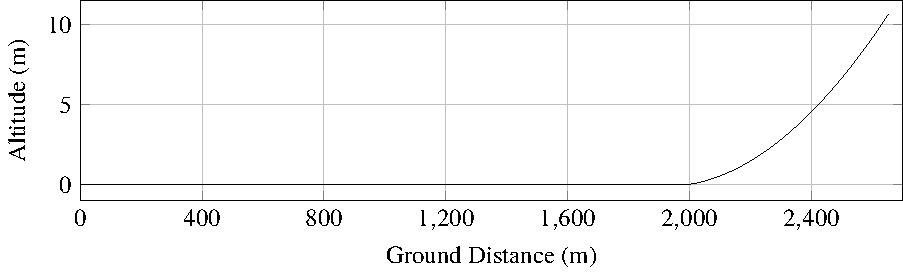
\includegraphics[keepaspectratio, width=1.1\textwidth]{TakeOff_Trajectory_OEI}
\caption{Take-off trajectory in OEI condition - ATR-72}
\end{figure}
%
\begin{figure}[H]
\centering
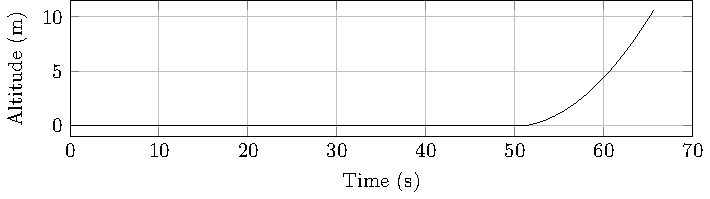
\includegraphics[keepaspectratio, width=1.1\textwidth]{Altitude_evolution_OEI}
\caption{Altitude evolution in OEI condition - ATR-72}
\end{figure}
%
\begin{figure}[H]
\centering
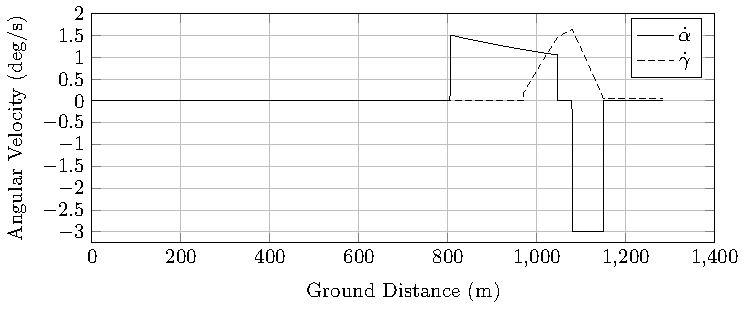
\includegraphics[keepaspectratio, width=1.1\textwidth]{AngularVelocity_vs_GroundDistance_AOE}
\caption{Angular velocities v.s. ground distance in AOE condition - ATR-72}
\end{figure}
%
\begin{figure}[H]
\centering
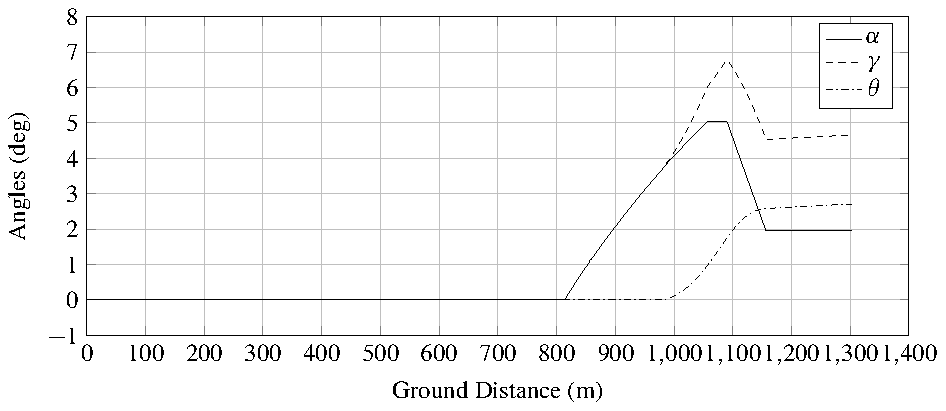
\includegraphics[keepaspectratio, width=1.1\textwidth]{Angles_vs_GroundDistance_AOE}
\caption{Angles v.s. grpund distance in AOE condition - ATR-72}
\end{figure}
%
\begin{figure}[H]
\centering
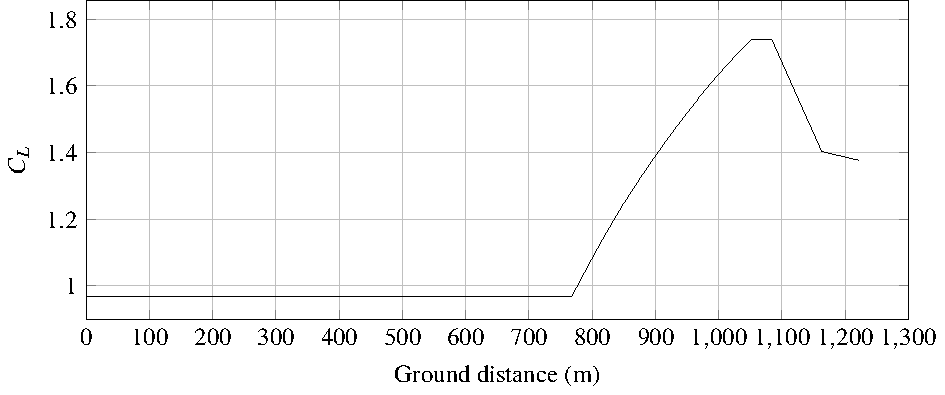
\includegraphics[keepaspectratio, width=1.1\textwidth]{CL_vs_GroundDistance_AOE}
\caption{$C_L$ v.s. ground distance in AOE condition - ATR-72}
\end{figure}
%
\begin{figure}[H]
\centering
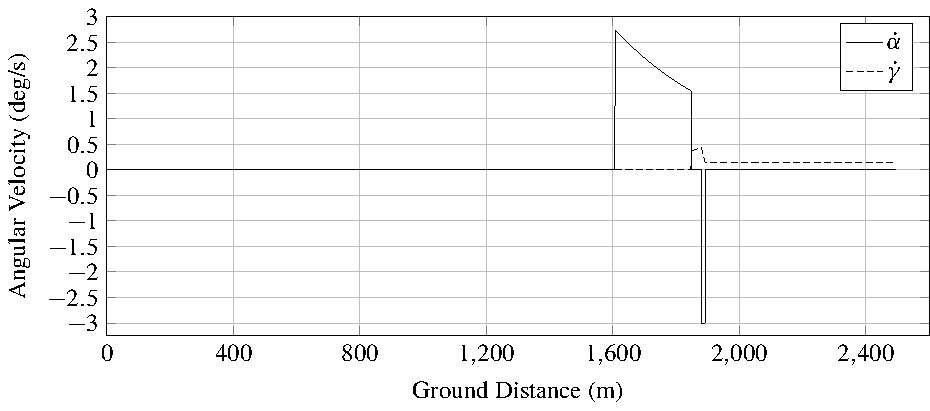
\includegraphics[keepaspectratio, width=1.1\textwidth]{AngularVelocity_vs_GroundDistance_OEI}
\caption{Angular velocities v.s. ground distance in OEI condition - ATR-72}
\end{figure}
%
\begin{figure}[H]
\centering
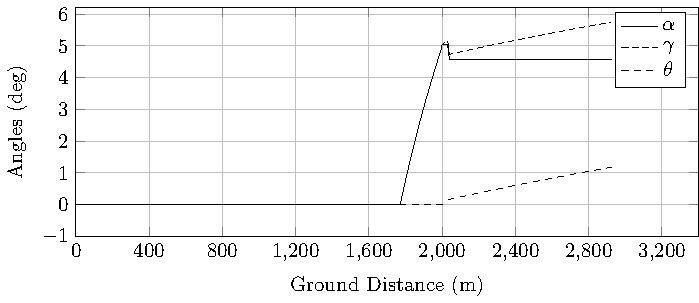
\includegraphics[keepaspectratio, width=1.05\textwidth]{Angles_vs_GroundDistance_OEI}
\caption{Angles v.s. ground distance in OEI condition - ATR-72}
\end{figure}
%
\begin{figure}[H]
\centering
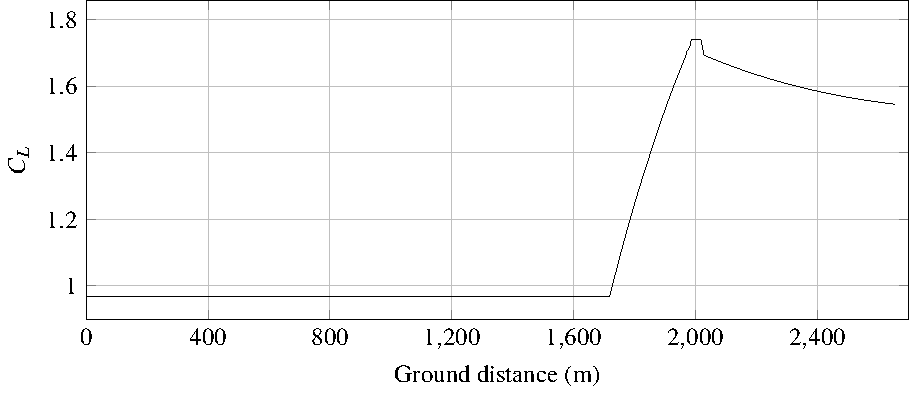
\includegraphics[keepaspectratio, width=1.1\textwidth]{CL_vs_GroundDistance_OEI}
\caption{$C_L$ v.s. ground distance in OEI condition - ATR-72}
\end{figure}
%
\begin{figure}[!t]
\centering
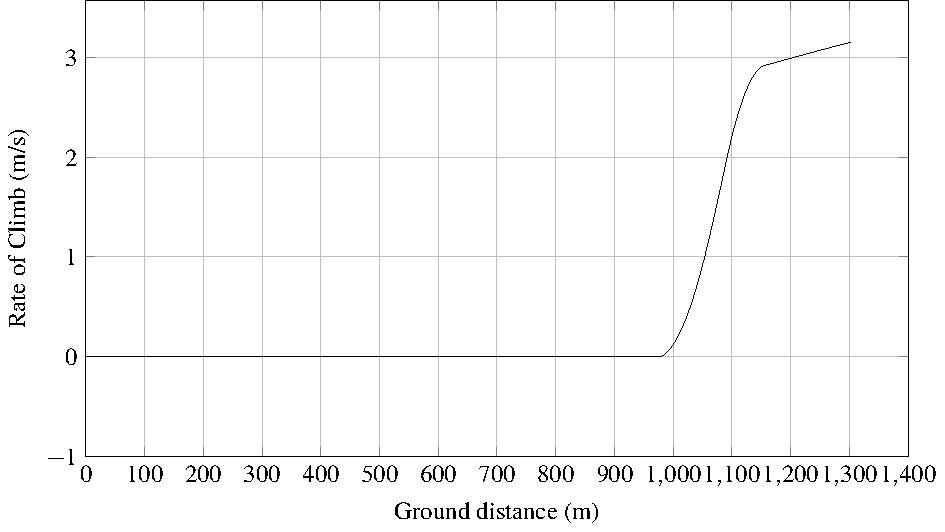
\includegraphics[keepaspectratio, width=1.1\textwidth]{RateOfClimb_vs_GroundDistance_AOE}
\caption{Rate of climb in AOE condition - ATR-72}
\end{figure}
%
\begin{figure}[!b]
\centering
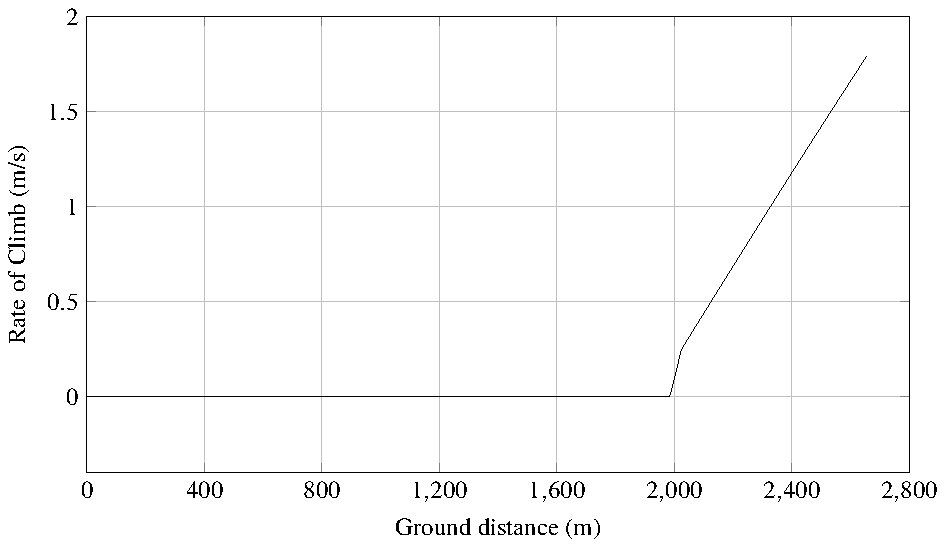
\includegraphics[keepaspectratio, width=1.1\textwidth]{RateOfClimb_vs_GroundDistance_OEI}
\caption{Rate of climb in OEI condition - ATR-72}
\end{figure}
%
\clearpage
%
\begin{figure}[H]
\centering
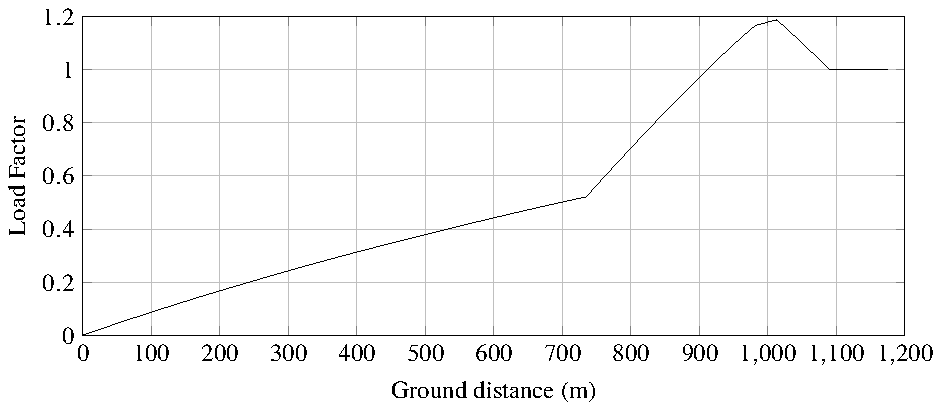
\includegraphics[keepaspectratio, width=1.07\textwidth]{LoadFactor_vs_GroundDistance_AOE}
\caption{Load factor in AOE condition - ATR-72}
\end{figure}
%
\begin{figure}[H]
\centering
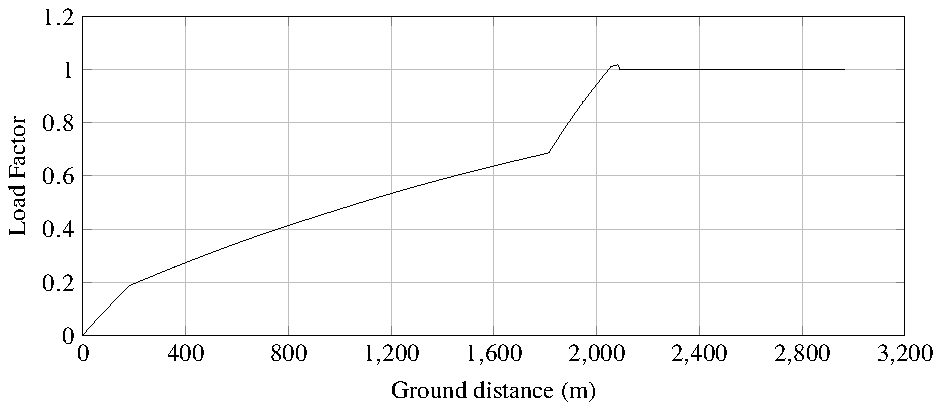
\includegraphics[keepaspectratio, width=1.07\textwidth]{LoadFactor_vs_GroundDistance_OEI}
\caption{Load factor in OEI condition - ATR-72}
\end{figure}
%
\begin{figure}[H]
\centering
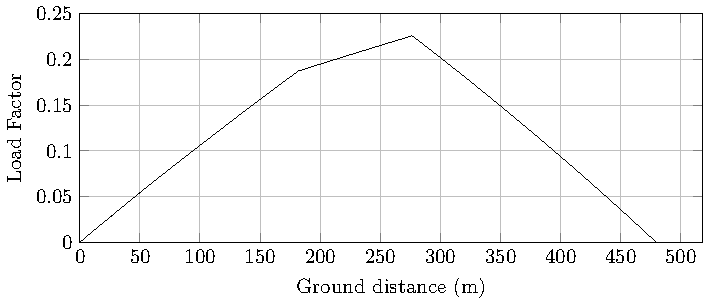
\includegraphics[keepaspectratio, width=1.05\textwidth]{LoadFactor_vs_GroundDistance_ABORTED}
\caption{Load factor in aborted take-off condition - ATR-72}
\end{figure}
%
\begin{figure}[H]
\centering
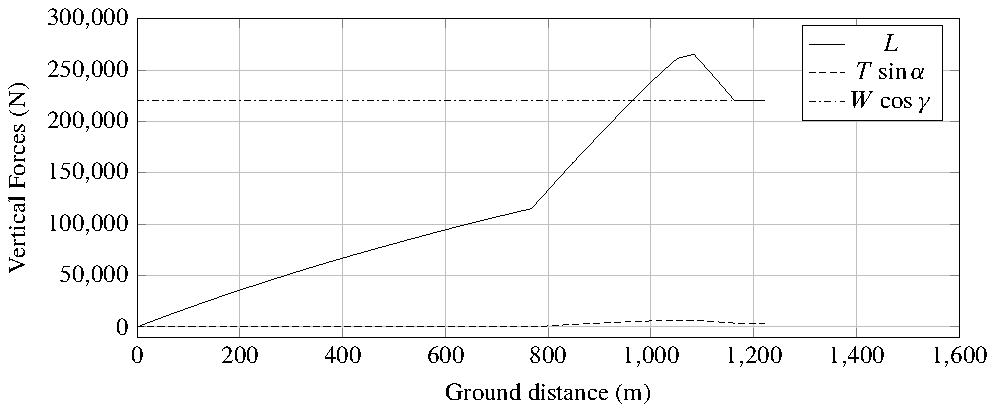
\includegraphics[keepaspectratio, width=1.1\textwidth]{VerticalForces_vs_GroundDistance_AOE}
\caption{Vertical forces in AOE condition - ATR-72}
\end{figure}
%
\begin{figure}[H]
\centering
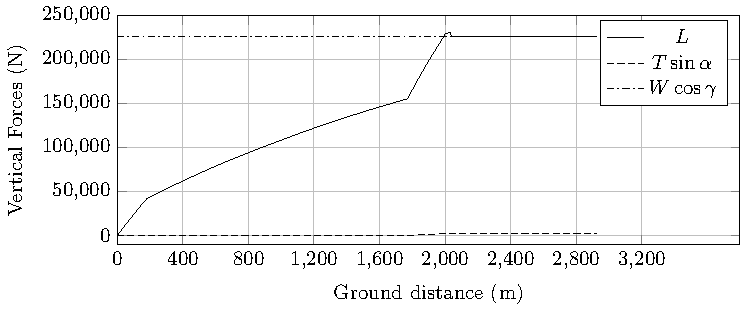
\includegraphics[keepaspectratio, width=1.1\textwidth]{VerticalForces_vs_GroundDistance_OEI}
\caption{Vertical forces in OEI condition - ATR-72}
\end{figure}
%
\begin{figure}[H]
\centering
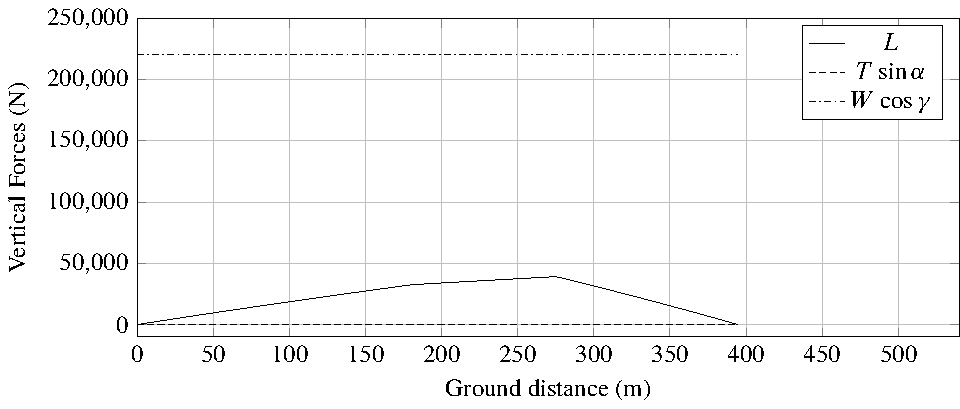
\includegraphics[keepaspectratio, width=1.1\textwidth]{VerticalForces_vs_GroundDistance_ABORTED}
\caption{Vertical forces in aborted take-off condition - ATR-72}
\end{figure}
%
\begin{figure}[H]
\centering
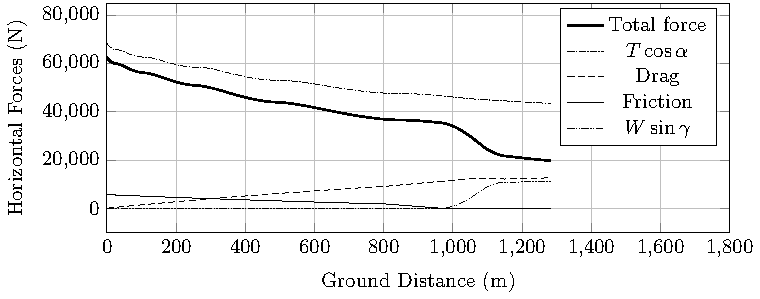
\includegraphics[keepaspectratio, width=1.1\textwidth]{HorizontalForces_vs_GroundDistance_AOE}
\caption{Horizontal forces in AOE condition - ATR-72}
\end{figure}
%
\begin{figure}[H]
\centering
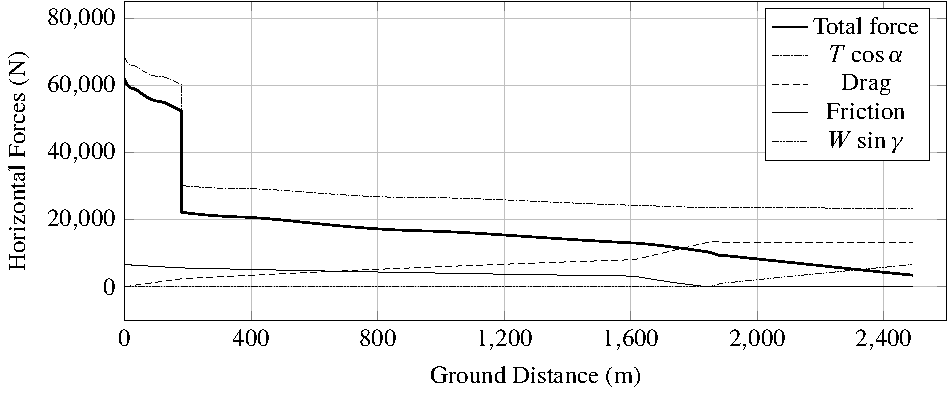
\includegraphics[keepaspectratio, width=1.1\textwidth]{HorizontalForces_vs_GroundDistance_OEI}
\caption{Horizontal forces in OEI condition - ATR-72}
\end{figure}
%
\begin{figure}[H]
\centering
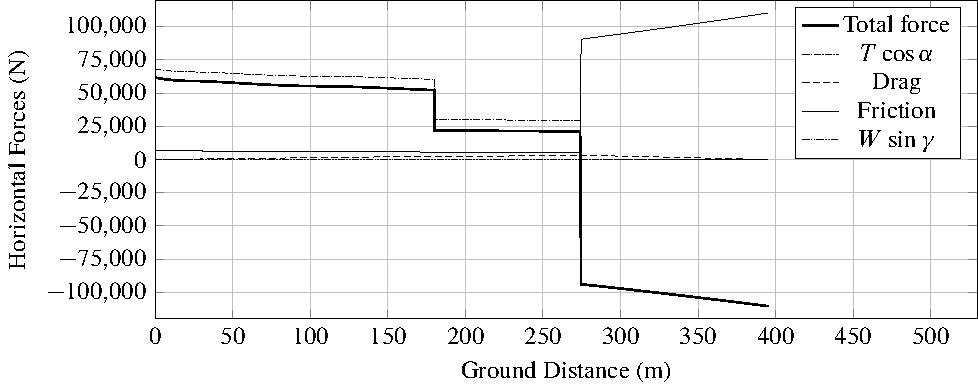
\includegraphics[keepaspectratio, width=1.1\textwidth]{HorizontalForces_vs_GroundDistance_ABORTED}
\caption{Horizontal forces in aborted take-off condition - ATR-72}
\end{figure}
%
\begin{figure}[H]
\centering
%Acceleration_vs_GroundDistance
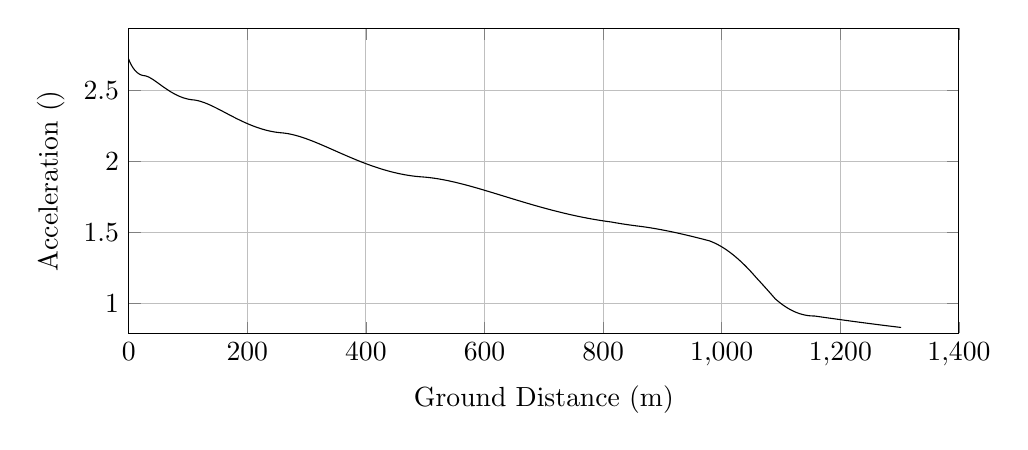
\begin{tikzpicture}

\begin{axis}[
width=\textwidth,
height=0.45\textwidth,
scaled ticks=false, tick label style={/pgf/number format/fixed},
xmin=0.0,
xmax=1400,
xlabel={Ground Distance (m)},
xmajorgrids,
ymin=0.7870546929072948,
ymax=2.9383329541999035,
ylabel={Acceleration ($\si{\meter\per\square\second}$)},
ymajorgrids
]

\addplot [
color=black,
solid
]
table[row sep=crcr]{
1.3603393307215537E-8	2.7206786612956035\\
2.0334443352841076E-7	2.7206786588266425\\
1.8493358258961232E-6	2.7206786374113054\\
9.983129263424352E-6	2.7206785316142303\\
4.13538327636676E-5	2.7206781237767137\\
1.2467543572893382E-4	2.720677041387967\\
2.843807411608912E-4	2.7206749688164837\\
5.588015241105573E-4	2.7206714118135586\\
9.398454696015893E-4	2.7206664793275745\\
0.0014155885812023746	2.720660329295151\\
0.0019945752038215015	2.7206528547539284\\
0.0026717822370171283	2.720644124141308\\
0.003447739291558293	2.7206341341019433\\
0.0043193476547732645	2.7206229279370353\\
0.00529092766782709	2.7206104535400364\\
0.006363550519206555	2.7205967007419662\\
0.007533073890550759	2.7205817261596685\\
0.008790616877968567	2.720565646667797\\
0.01016549189277427	2.7205480911659583\\
0.011625499440327931	2.7205294744355797\\
0.013184282533086976	2.72050962565101\\
0.014839871214038253	2.7204885733470565\\
0.01660567024659266	2.720466150823441\\
0.018465948346479452	2.7204425615356786\\
0.0203822997817096	2.7204182947581463\\
0.022430561433814646	2.720392393417905\\
0.024588423902376283	2.7203651442989134\\
0.026831028501027587	2.7203368647401236\\
0.029143159681622913	2.7203077489819503\\
0.03155709159958957	2.7202773934304583\\
0.03411445662773917	2.7202452793221816\\
0.03677290089167576	2.720211943282595\\
0.03952314881844239	2.7201775050183548\\
0.04239921643077808	2.720141542640251\\
0.045357163155895136	2.7201046093765235\\
0.048363831658398165	2.720067120971648\\
0.051533845233668635	2.7200276521592013\\
0.0547899150155587	2.719987170149106\\
0.058172599437445835	2.7199451746177328\\
0.06162834747858026	2.719902333979718\\
0.06521401059050522	2.719857947124008\\
0.06888104003120077	2.7198126189354435\\
0.07268727020998902	2.7197656386724027\\
0.076546425570032	2.7197180746221186\\
0.08047032364859658	2.7196697825197393\\
0.08456364881336098	2.719619478509671\\
0.08882250397434277	2.7195672177387413\\
0.09306368907640691	2.7195152504659523\\
0.09743039119190974	2.7194618233250623\\
0.10191450167634594	2.719407040285338\\
0.10651989152467789	2.719350858705292\\
0.11128201757858264	2.719292851771846\\
0.11609763023253863	2.7192342810465364\\
0.12097769621339591	2.7191750145198688\\
0.12591912973280778	2.719115091275551\\
0.13103216605369056	2.7190531790214214\\
0.13633380151185176	2.7189890799222596\\
0.1416823117522269	2.7189245120751977\\
0.14708837902374172	2.718859347520925\\
0.1525605467319851	2.718793484820159\\
0.15824953188605478	2.7187251158179464\\
0.16398006351864292	2.718656352093608\\
0.16978153473626356	2.7185868421723756\\
0.17584258400626962	2.7185143330821866\\
0.1819863832139092	2.718440947782791\\
0.18819485651962437	2.7183669043448937\\
0.19455736971520038	2.7182911411090585\\
0.20098158490654017	2.7182147616689916\\
0.2076061353991409	2.718136123110612\\
0.21424726384720844	2.718057410870288\\
0.2211374965027113	2.7179758744402864\\
0.2281284453493247	2.717893277608118\\
0.2350833915765042	2.7178112355168347\\
0.2423085249848444	2.7177261408549382\\
0.24958374984531584	2.7176405928122973\\
0.2569279402934431	2.7175543707998235\\
0.2644720218029696	2.717465943282936\\
0.27204626263318243	2.7173773042321585\\
0.27972793364503945	2.7172875512397434\\
0.2874622320100655	2.7171973271364305\\
0.29563698092580604	2.717102119683042\\
0.30361763245720474	2.7170093241059803\\
0.3118912000478351	2.7169132783506376\\
0.3202493147046803	2.7168164099718446\\
0.3286412952843002	2.7167193076559375\\
0.33714554464307567	2.716621066313662\\
0.3458731203690518	2.716520410471115\\
0.35455185683415313	2.7164204819449873\\
0.3634323904331427	2.7163183971483607\\
0.372325738896249	2.716216332541263\\
0.38151551889959867	2.7161110399165134\\
0.3908489672358084	2.716004280047283\\
0.4001862088113266	2.7158976550020775\\
0.4095647137707429	2.7157907361040916\\
0.4192312859369268	2.7156807169939983\\
0.4289206911602753	2.7155706232017947\\
0.43896550245304145	2.7154566846950363\\
0.4487817299761361	2.7153455272169174\\
0.4589033974758888	2.7152311036303827\\
0.4691858798479248	2.715115060160417\\
0.47972601481223376	2.7149963139012074\\
0.49016040525287174	2.7148789611485267\\
0.5007175269203565	2.714760430608898\\
0.511266977039379	2.714642187576308\\
0.522323236324642	2.7145184777830185\\
0.5332586746953114	2.7143963328736067\\
0.5445869154512923	2.7142700215729363\\
0.5556699580072249	2.7141466597700834\\
0.5669225885056133	2.714021626213362\\
0.5785590177532589	2.713892554574162\\
0.5903083066022885	2.713762462426807\\
0.6020327889628274	2.7136328743733085\\
0.613957077533064	2.713501310690825\\
0.625960998969677	2.7133691032213507\\
0.6380070243193761	2.713236666618247\\
0.6503365955459197	2.713101353706329\\
0.662700086001522	2.712965911112848\\
0.6752747602080436	2.7128284018285003\\
0.6885889407972636	2.7126830744997443\\
0.7019767933734617	2.7125372191246226\\
0.7151149754112038	2.712394350438487\\
0.7284684478906998	2.7122494087541904\\
0.7418939875700234	2.712103954863111\\
0.7553494584716574	2.711958445905217\\
0.7694215958599202	2.7118065539718383\\
0.7830840331449673	2.7116593612657827\\
0.796657372658726	2.7115133963344817\\
0.8106660034246236	2.711363027941603\\
0.8251837647136968	2.7112074894914313\\
0.8395067871054176	2.7110543290584967\\
0.8540519574023793	2.7108990870358225\\
0.8688334527125461	2.7107416235367525\\
0.8840141863517745	2.7105802200273583\\
0.8993797082767976	2.7104171720264008\\
0.9143697020410035	2.7102584166704773\\
0.9294094610857999	2.7100994372507596\\
0.9452486359568626	2.7099323329379637\\
0.9605773823977486	2.709770928967991\\
0.9761522209726621	2.7096072488307197\\
0.9917649966835071	2.709443486198965\\
1.0074810114554809	2.7092789578986203\\
1.0234652146968335	2.7091119458674218\\
1.0399433598517231	2.7089401120912475\\
1.0563627364420554	2.708769231027813\\
1.0728309985448887	2.708598179325757\\
1.0896486452479222	2.7084238454325265\\
1.1068138420051672	2.7082462673532888\\
1.124143995869574	2.708067347375602\\
1.1415400048645106	2.707888113111455\\
1.1590089082607062	2.7077084936001095\\
1.1769249919091855	2.707524653931576\\
1.1951505705127592	2.7073380281037513\\
1.2127191877709298	2.7071584985763346\\
1.2308827453761335	2.706973267662627\\
1.2492706857898845	2.706786137242294\\
1.267587852451018	2.706600113080426\\
1.2860031245644312	2.7064134781225864\\
1.304687144125951	2.7062245116829278\\
1.3233765774990474	2.7060358828879156\\
1.342322280991234	2.7058450653162245\\
1.3613696045164358	2.705653625031875\\
1.3815086998747366	2.7054516455381066\\
1.4013123019267382	2.7052534626110045\\
1.4209622886438908	2.7050572371882557\\
1.4411501686096515	2.704856073193203\\
1.4611760119255748	2.7046569542278975\\
1.4816444281325132	2.704453874606884\\
1.501865958841821	2.704253678164765\\
1.5224364680875304	2.704050466014486\\
1.543651615594651	2.7038413464626005\\
1.5647593029468103	2.70363374738879\\
1.5859558716309676	2.7034257339559584\\
1.6071423964076703	2.7032182764344252\\
1.6293386351549652	2.703001418962213\\
1.6508498980272122	2.7027917261443655\\
1.673011606043147	2.7025761758197744\\
1.6946435720294923	2.702366247606573\\
1.717066624993247	2.702149128823603\\
1.739432891071898	2.7019330500985044\\
1.761922286799709	2.7017162722331785\\
1.7849035550437842	2.7014952578520406\\
1.8076299607761817	2.70127719298858\\
1.8313298306791497	2.7010503120862657\\
1.8543134894513886	2.700830795787314\\
1.8777326664639729	2.7006076313435097\\
1.9017196849182967	2.7003795876766175\\
1.925345883672024	2.7001554970834443\\
1.950252961491087	2.699919815747629\\
1.975161211119453	2.6996846926241336\\
1.9993825790313986	2.699456595879024\\
2.024583888346972	2.699219835107348\\
2.04934017380271	2.6989878120385447\\
2.0744229633459703	2.698753288188291\\
2.0996193404956136	2.6985182656177127\\
2.1245764901457758	2.698286027665972\\
2.1500786393425866	2.6980492835167134\\
2.176226227020705	2.6978071372330295\\
2.202115608176549	2.697567966791156\\
2.227948363055355	2.697329895830868\\
2.2543499999408594	2.697087173470252\\
2.2810892744412783	2.6968419527082137\\
2.3075963743135786	2.696599459185051\\
2.3348582111613405	2.6963506785209344\\
2.3623221378972126	2.696100682933973\\
2.3898598419727675	2.695850646147277\\
2.4171687299087603	2.6956033066724263\\
2.445442108612223	2.6953478780856788\\
2.4735885391813177	2.695094245735042\\
2.5015416452491293	2.694842992960848\\
2.5301110763218357	2.694586853096574\\
2.5589284934403693	2.6943291544481216\\
2.587611617795936	2.6940733156453813\\
2.6175687086884984	2.6938068114957927\\
2.647724154312196	2.6935392585977587\\
2.6767118187859253	2.6932827399161683\\
2.7060305938995466	2.693023958539718\\
2.7361546404224653	2.6927587646133873\\
2.7663022704956823	2.6924940645077875\\
2.7964672462043376	2.6922299104775878\\
2.8272583584284883	2.6919609898244374\\
2.8588650092419234	2.691685695066152\\
2.8898852960400587	2.6914162407917983\\
2.9215246589961597	2.691142153042156\\
2.95270311230069	2.6908727891002586\\
2.984506337549637	2.6905987709596655\\
3.017379145769185	2.6903163220215216\\
3.049243647754313	2.6900432938557373\\
3.081295157663824	2.6897694112189523\\
3.113406837946715	2.6894957625659544\\
3.1453724573084756	2.6892240983894453\\
3.1787286104953543	2.688941399310255\\
3.211019796961401	2.6886684834859587\\
3.245786703184362	2.688375472165572\\
3.279939251746722	2.688088470588985\\
3.3141720228361216	2.6878016178550492\\
3.3491198891036547	2.687509618361971\\
3.382965192547779	2.68722764086513\\
3.4181848705561064	2.6869350544215695\\
3.45391888941694	2.6866390675413285\\
3.488851494856137	2.686350563708105\\
3.524271454997704	2.6860588832442085\\
3.5606552075305	2.6857601507740503\\
3.597189071478943	2.6854610832006927\\
3.632926148839256	2.6851694036217726\\
3.668897146318187	2.6848766746939123\\
3.706642714683163	2.6845704271949034\\
3.7432264628550644	2.684274503176929\\
3.781286297809391	2.6839675714925635\\
3.818618572105483	2.6836674260810867\\
3.8564015479305356	2.683364578880271\\
3.8948624022541356	2.683057245696653\\
3.9329637046009225	2.682753723357327\\
3.971505929995028	2.6824476332723757\\
4.009821706071438	2.682144278613734\\
4.049014376833089	2.68183494307692\\
4.089343885784727	2.6815176449538445\\
4.128662304630717	2.681209283054529\\
4.1684827283974055	2.6808979665822283\\
4.208000253554632	2.6805899907618347\\
4.2483743636521965	2.680276334838056\\
4.288255503180503	2.6799674917027794\\
4.328757204126676	2.679654837844873\\
4.369490126907612	2.6793414053306783\\
4.410357715197167	2.679027945740783\\
4.45189144941496	2.6787104072993566\\
4.492881116440694	2.678398042025564\\
4.53550011161515	2.678074322825818\\
4.577670191557685	2.6777550743742067\\
4.6201174049766305	2.677434788405729\\
4.662272021613388	2.677117758143571\\
4.706017761800355	2.6767898603786255\\
4.748842845578064	2.6764699422389615\\
4.792293145132742	2.6761464390631\\
4.836482439768313	2.6758185498568317\\
4.88090298307878	2.6754900735892466\\
4.925311889063089	2.675162809239379\\
4.969864686447545	2.6748356102636386\\
5.014842280541593	2.674506429836776\\
5.0603877575117515	2.674174253072983\\
5.106292347304597	2.673840632515052\\
5.152263975081851	2.6735077016112054\\
5.1974808794106995	2.673181379928213\\
5.244027372436168	2.6728466417574968\\
5.28996242022761	2.672517467815287\\
5.336209145350672	2.672187226039256\\
5.38320569473032	2.6718528225038405\\
5.430469292142472	2.6715177256382523\\
5.476900151253712	2.6711897058694722\\
5.526063828851289	2.6708436409213805\\
5.573879040902945	2.670508306612775\\
5.622613575936374	2.6701677760662514\\
5.6713596863799225	2.669828422251273\\
5.720412183296268	2.6694881992513135\\
5.770660497446668	2.669140990560754\\
5.820668144990444	2.6687967533759176\\
5.870305285939629	2.6684563516020408\\
5.920503816994749	2.668113395941104\\
5.971105439367246	2.6677689993918303\\
6.021088325934068	2.6674301023059055\\
6.071322359863801	2.6670907866316345\\
6.122981826035449	2.6667431793464864\\
6.174329110820436	2.6663990098143406\\
6.225804784288178	2.666055311784361\\
6.278093246139479	2.665707546198239\\
6.331709873490098	2.6653523633215936\\
6.384325657889258	2.665005198295482\\
6.436648686434458	2.6646613220440125\\
6.489478972803882	2.6643154790220605\\
6.543185721519176	2.663965300169796\\
6.596747696432654	2.6636174666252757\\
6.650345873843312	2.663270792682101\\
6.704555155195255	2.6629215790004643\\
6.7588986063680725	2.6625729209380244\\
6.814371620173711	2.6622184756758003\\
6.86997180120154	2.661864691332725\\
6.925426612865756	2.6615132948772278\\
6.981353650685165	2.6611603793268515\\
7.037678624474159	2.660806441464639\\
7.094603706786671	2.660450243996549\\
7.151204881983983	2.6600975732102974\\
7.209200593921791	2.659737757917874\\
7.2667780016693655	2.65938207763521\\
7.324687293141565	2.6590258879349387\\
7.382771066065313	2.65867017051857\\
7.441904508776327	2.658309607849323\\
7.501585831803217	2.6579473170852808\\
7.5616527251378685	2.657584314371988\\
7.62150963104709	2.657224198940635\\
7.682859947113334	2.656856767854337\\
7.7432084367972145	2.656496978162604\\
7.803024936926759	2.656141959652575\\
7.863793829029664	2.6557829123419427\\
7.9252460466886365	2.655421484914137\\
7.98696966925656	2.655060131675171\\
8.04776546969778	2.654705839910287\\
8.109421212326083	2.654348181634318\\
8.17269125419024	2.6539828737863242\\
8.236095044780246	2.6536185288074092\\
8.299523592514586	2.65325577215485\\
8.363213767675873	2.652893253529224\\
8.427807923256076	2.6525273571081653\\
8.49144930156071	2.6521685912907564\\
8.557380457258176	2.651798724322129\\
8.623183572921022	2.6514314015421423\\
8.687840683575093	2.6510722452291935\\
8.753751426394068	2.6507079228346413\\
8.820803713780364	2.6503391450473472\\
8.888970287482593	2.649966148101651\\
8.957133699158991	2.649595085188113\\
9.025036015045707	2.6492273412772986\\
9.092760955867519	2.6488624367385345\\
9.159817422823458	2.648502974954302\\
9.227495373767134	2.6481420314749275\\
9.296013084156197	2.6477784947261016\\
9.36435980631623	2.6474177474136527\\
9.433329865923408	2.6470556079181042\\
9.503849553921977	2.6466872950515414\\
9.574524061692681	2.6463201570111243\\
9.644263228942293	2.645959816265661\\
9.715657612596786	2.645592909530688\\
9.787429657508813	2.645226079457479\\
9.85753688572494	2.6448697034479203\\
9.930250735750551	2.644502099823873\\
10.001571447096964	2.6441435319093944\\
10.074699859091687	2.643777916552698\\
10.14698611653175	2.6434185343790606\\
10.220547980738981	2.6430548666019744\\
10.2940409891517	2.642693602309274\\
10.36719293590382	2.642336054188199\\
10.441008888975666	2.6419773151014647\\
10.51610421670324	2.641614467762291\\
10.590724589239105	2.6412560143644788\\
10.667218005391902	2.6408907266274424\\
10.742771202259895	2.640532070108522\\
10.82035208750042	2.6401659936636683\\
10.896759047300378	2.6398076323121202\\
10.973503045910835	2.6394498550940453\\
11.051297940743765	2.6390893843891003\\
11.128076326409062	2.6387357926937325\\
11.207667705350879	2.6383715117432622\\
11.286758396846047	2.638011798043455\\
11.366305937658339	2.6376522856971496\\
11.446149720998452	2.637293723994773\\
11.526866579636565	2.636933563877787\\
11.607297517600138	2.6365769930935956\\
11.688034241538357	2.6362213802710963\\
11.769665722224765	2.6358641739102344\\
11.850920080706608	2.635510952816559\\
11.933163326324259	2.635155796089923\\
12.017103780766782	2.6347957522379453\\
12.10034832931326	2.6344411202567057\\
12.185467765774142	2.6340809903748106\\
12.270669986481685	2.6337230211751725\\
12.354040133273898	2.633375171561526\\
12.440386807402234	2.6330174188864603\\
12.52556588630658	2.6326670026774126\\
12.610860989997974	2.6323185865436374\\
12.69550109439961	2.631975287279447\\
12.784634337461807	2.631616382824756\\
12.871172079509357	2.6312704900596824\\
12.958447214271366	2.630924195280638\\
13.045518554761987	2.6305812467301823\\
13.133090172249581	2.6302388746430134\\
13.221405510214687	2.629896172019415\\
13.310319106907201	2.6295537524618187\\
13.399783591735492	2.629211839154097\\
13.488943611067967	2.628873702111904\\
13.578276665194153	2.6285375149135355\\
13.667402973129146	2.6282046957139578\\
13.757763665999576	2.627869898230623\\
13.848393619195729	2.627536754471522\\
13.938857764339925	2.627206858503314\\
14.031101516310692	2.6268731770392186\\
14.123507833735925	2.6265416352199544\\
14.214825187590282	2.6262166726791465\\
14.307956552027534	2.625887980862263\\
14.401498558574918	2.625560600783583\\
14.495315613017755	2.6252350272686176\\
14.589065423003394	2.624912447314662\\
14.68316852398955	2.6245914165312207\\
14.778702641747682	2.624268327122402\\
14.873746415615575	2.6239497085396195\\
14.970384078097169	2.623628612553521\\
15.068900921005241	2.6233042363691323\\
15.164434274206265	2.6229925309927165\\
15.260378587808539	2.622682296359665\\
15.357189194448868	2.6223721064177115\\
15.45495288999333	2.6220617534077197\\
15.55311774366497	2.621753039337219\\
15.652583807013901	2.6214431992530205\\
15.755243917873962	2.6211265293566273\\
15.855950289561445	2.620818954146916\\
15.958461094374158	2.620508977405793\\
16.060387288500337	2.620203867681534\\
16.164276126126843	2.6198960517212635\\
16.26736468838029	2.6195937578082233\\
16.36946523634058	2.619297443871246\\
16.47192386662276	2.619003163968875\\
16.576794358652606	2.618705133782723\\
16.678929175716583	2.61841795664116\\
16.783994526910618	2.6181256984077486\\
16.89012564586595	2.6178337166503045\\
16.996887404888547	2.6175432749417187\\
17.103774697793426	2.6172557707268638\\
17.210947675936964	2.6169707806812017\\
17.31865021419634	2.6166876823252405\\
17.424470519881233	2.6164127421635106\\
17.53205215515201	2.6161364768833204\\
17.64034909906897	2.6158616741719065\\
17.74911485075183	2.615589002397387\\
17.85745376408675	2.6153206975844308\\
17.969383314157206	2.6150469444401168\\
18.07998395718984	2.614779867810088\\
18.18863741327577	2.6145207984136016\\
18.302466989554325	2.6142528890063197\\
18.41305080779906	2.6139960386827914\\
18.525644000014054	2.613737972345975\\
18.636945827420575	2.6134862769421234\\
18.750643923449367	2.6132326526951157\\
18.86479622056296	2.612981551792113\\
18.979646899421056	2.6127324788448334\\
19.09418630108147	2.6124876296228825\\
19.208983505033515	2.612245773334588\\
19.323483295898072	2.6120080662516196\\
19.43842354827664	2.6117729715390476\\
19.55563752357537	2.6115368534254326\\
19.67199913451129	2.611306063351325\\
19.789486593639566	2.611076678576726\\
19.90713985662446	2.610850621722009\\
20.024127533725753	2.610629455253049\\
20.143019013955552	2.610408367403082\\
20.26442367074238	2.6101864195670723\\
20.383660776265387	2.609972172998143\\
20.5042342316437	2.6097592805638037\\
20.622773342122727	2.609553649589869\\
20.74503732713029	2.6093453564489195\\
20.865944869938517	2.6091431563868124\\
20.98711015528624	2.608944286470133\\
21.113336299999695	2.6087411017443536\\
21.23638685227678	2.608546937145694\\
21.35988644990264	2.6083559314440388\\
21.483760012473958	2.608168227292362\\
21.608180515260266	2.607983593725539\\
21.732326713270083	2.607803250150675\\
21.85766379468624	2.607625099075144\\
21.985117186778353	2.607447968969981\\
22.111729024702363	2.6072760185911354\\
22.23700541150786	2.607109803648334\\
22.36297326225872	2.606946592655331\\
22.488604760551	2.6067877220942135\\
22.616276341350805	2.6066302545800575\\
22.744235570279145	2.606476448725659\\
22.874576476768283	2.606323901548314\\
23.003842066605536	2.6061767086234635\\
23.13088450205612	2.606036009470011\\
23.257869280739328	2.6058992879025347\\
23.389244224935425	2.6057619455713583\\
23.519811196806458	2.605629573115798\\
23.653309395988643	2.6054984682974673\\
23.78342402399784	2.6053747991575955\\
23.9180644861338	2.6052510900680304\\
24.05110504604577	2.60513309614823\\
24.182394801971697	2.6050207798574423\\
24.314614014384034	2.6049117976909457\\
24.449791085561472	2.6048046491534915\\
24.585258581909038	2.604701590808493\\
24.72121222319008	2.6046024984638763\\
24.857032405393277	2.6045078282062573\\
24.99454740444294	2.60441636799246\\
25.13030709358258	2.6043303973208944\\
25.270890409679986	2.604245885116941\\
25.40663839363527	2.604168625105072\\
25.54307796688363	2.6040952615282915\\
25.68272814639034	2.604024613245566\\
25.82072003425767	2.603959205279013\\
25.96015212691003	2.603897546240571\\
25.987750021099068	2.6038858690712825\\
26.0558803939429	2.6038577864228225\\
26.061632797568386	2.6038554638263935\\
26.066808273335674	2.6038533806198574\\
26.071901058608013	2.6038513366596883\\
26.073315434863225	2.6038507697843425\\
26.074595035914804	2.6038502564501425\\
26.080371168076944	2.6038479331864\\
26.10234540095133	2.603839004048819\\
26.183408179590366	2.6038048263627918\\
26.300430535410044	2.6037520750387655\\
26.42750601924636	2.603690272544413\\
26.558056987479794	2.6036219372736085\\
26.688030995483615	2.603549088212217\\
26.818767077324992	2.6034710242918466\\
26.951519978077492	2.6033869035939228\\
27.083955405447817	2.603298172686217\\
27.216897884715692	2.603204329397653\\
27.350913258119895	2.6031049498085697\\
27.4833530065795	2.6030020840485344\\
27.6176201223548	2.602893135321435\\
27.752160408628434	2.6027793145137146\\
27.887329802382908	2.6026603332918947\\
28.023188645890663	2.6025361303873034\\
28.158973127824495	2.6024074319911854\\
28.296372294036907	2.602272619137292\\
28.435107205966254	2.6021318778665234\\
28.571323599682245	2.6019892357069097\\
28.70996262687553	2.6018395823204976\\
28.850320389600306	2.6016835359128985\\
28.988837241064125	2.6015251189808373\\
29.129197813929657	2.6013601767352137\\
29.27166529868488	2.60118827267934\\
29.41298471572133	2.60101334901779\\
29.554848516656044	2.6008333985884082\\
29.699676691743235	2.6006452500398893\\
29.842400551696755	2.6004555085017884\\
29.985385440862252	2.6002611719940534\\
30.129077275410303	2.600061649734757\\
30.27543774584293	2.5998541279415415\\
30.422081339040986	2.599641919100981\\
30.56949149516445	2.599424338278923\\
30.716562179458485	2.599203059515774\\
30.86535310281699	2.5989749850175308\\
31.011875026602333	2.5987463115259466\\
31.16159928701196	2.5985085205974414\\
31.313692569485013	2.598262765131782\\
31.463056706803336	2.598017357590823\\
31.61235366859384	2.597768096492202\\
31.76278957628285	2.5975129835032753\\
31.915019899787076	2.5972508499553557\\
32.06709627595497	2.5969850453468277\\
32.21861178877769	2.5967163665556434\\
32.37168228565527	2.596441081645162\\
32.52450570609457	2.596162439682959\\
32.67702483599189	2.5958806223094966\\
32.829998687403204	2.5955942777679697\\
32.98551220909506	2.5952994517569667\\
33.14332298937855	2.5949964875960214\\
33.29970221124884	2.5946925710318984\\
33.45800124694219	2.594381230122983\\
33.61398946945653	2.59407085606417\\
33.77048353048475	2.5937559624467577\\
33.9292721471582	2.593432911844313\\
34.08796840843395	2.5931065431041294\\
34.24769686644211	2.5927745690501176\\
34.406855482575295	2.592440360126446\\
34.56481953291838	2.5921053392665625\\
34.72399692808165	2.591764453104413\\
34.88694269464703	2.591412129924282\\
35.04914399338672	2.591058089493738\\
35.209965099803895	2.590703839194963\\
35.3703140559587	2.590347487556378\\
35.531685786905925	2.589985748967039\\
35.69349909442164	2.589619936461779\\
35.85522798807463	2.5892512811122277\\
36.022509111806116	2.5888668336311342\\
36.19055880791667	2.588477464988384\\
36.35708622463872	2.5880885595397194\\
36.52115360367851	2.5877024693187627\\
36.68781562330062	2.5873073486572045\\
36.8536847754776	2.586911233267797\\
37.024522648961764	2.586500308629536\\
37.19188554678789	2.5860948991511465\\
37.36066720850286	2.585683255555418\\
37.528862119520696	2.585270300070748\\
37.697264258302326	2.584854143682125\\
37.86832931534104	2.5844287005776634\\
38.03812867477943	2.5840037593985663\\
38.20923731912278	2.5835729261965747\\
38.37904730305398	2.5831428173348794\\
38.55252405124031	2.5827008536311844\\
38.72282139824354	2.5822645157823274\\
38.89783411301201	2.5818135931288113\\
39.0714610757495	2.581363784250743\\
39.24438070689564	2.580913425517954\\
39.41969314875929	2.5804544577618174\\
39.59166556575205	2.580001956794118\\
39.764623188591585	2.579544636010196\\
39.94263254662576	2.5790716744061593\\
40.11749159802578	2.578604876133886\\
40.29452954971913	2.5781300814298502\\
40.47247750600427	2.5776506846058913\\
40.64799609178485	2.577175756740913\\
40.82414741101539	2.57669709043791\\
41.00385670225303	2.576206711349962\\
41.18169069533937	2.575719463467573\\
41.3603281005193	2.575228071765099\\
41.54046179251334	2.57473063920484\\
41.722675278204306	2.5742255441599875\\
41.90258931008478	2.573724975558771\\
42.08518735141125	2.5732151086952273\\
42.26728550944881	2.572704847119067\\
42.44743534848537	2.5721983302188898\\
42.63069538383506	2.5716813637181577\\
42.80963512098974	2.5711749685245957\\
42.992542679335614	2.5706557379097825\\
43.17926890616222	2.5701240368278295\\
43.363134036078335	2.5695989178025833\\
43.54815051311773	2.5690689872462267\\
43.733578141849236	2.5685363896694895\\
43.91798130912079	2.568005298831979\\
44.10506009255049	2.5674650822870673\\
44.29251116260117	2.5669223997879653\\
44.480917546793805	2.5663755921121174\\
44.66851287589745	2.565829826985854\\
44.85853501730759	2.565275710745273\\
45.047396872181054	2.5647237332038157\\
45.236914792155844	2.5641686329837823\\
45.42785879536018	2.5636081770353583\\
45.616432631699865	2.563053557848849\\
45.80697204128492	2.5624920680802825\\
45.998633580597016	2.561926207731924\\
46.18800675699903	2.561366095611291\\
46.380841640082096	2.560794755738124\\
46.57327038933336	2.560223664626961\\
46.765844918266424	2.559651226210809\\
46.95911042680183	2.5590758535903007\\
47.15311668852311	2.5584974283805613\\
47.34541611633634	2.5579232929457483\\
47.53884854699059	2.5573450104603674\\
47.73236991243341	2.5567657329192537\\
47.92818250719388	2.5561788929077913\\
48.12326385407131	2.555593578167602\\
48.32058854034828	2.5550008943769527\\
48.516852452700604	2.554410797753267\\
48.71339374517507	2.5538193058348817\\
48.91319881343868	2.5532174537276386\\
49.1119162355681	2.552618377571118\\
49.31207818344666	2.552014479879058\\
49.509673461222235	2.55141790295568\\
49.71156302510582	2.550807963814867\\
49.91034548441702	2.5502070557604366\\
50.11200805970151	2.5495971167179245\\
50.30853267551517	2.549002437643254\\
50.50757456960626	2.548399893787912\\
50.70929197287772	2.547789031091562\\
50.91222418686718	2.547174301781091\\
51.11562549758783	2.5465579976334327\\
51.32090674103446	2.545935876599027\\
51.525199701657655	2.545316665210681\\
51.72863462744459	2.544700004051853\\
51.934060761332375	2.5440772901396684\\
52.14033810224923	2.5434520130707616\\
52.344882977561255	2.542832037968295\\
52.55098100649393	2.5422074393837404\\
52.75731843494604	2.541582232938185\\
52.96514817708821	2.5409526569511103\\
53.17450540782369	2.540318641605455\\
53.382202621450276	2.5396898725022634\\
53.592230583406476	2.5390543021876466\\
53.80364534107798	2.5384148270146696\\
54.01469481143569	2.5377767815041166\\
54.223966920081466	2.537144461612022\\
54.43230789395902	2.5365153346114173\\
54.6430562980421	2.5358793541120868\\
54.855225786754914	2.5352395392705507\\
55.066088958624874	2.5346041459414534\\
55.27969530828261	2.5339610077522634\\
55.49171188337613	2.5333232052728736\\
55.70388919125476	2.532685496995895\\
55.91737779085577	2.532044460808315\\
56.13177028494084	2.531401359471393\\
56.34652664868587	2.5307578484066866\\
56.559021044851505	2.530121815748167\\
56.77591447970492	2.5294733639353444\\
56.99548236897459	2.5288177159078513\\
57.21481285737903	2.5281636101320872\\
57.43536222847358	2.5275067392423107\\
57.65367025761124	2.526857432179728\\
57.872788904232735	2.5262066317271605\\
58.0907693980174	2.525560152036414\\
58.311927420720366	2.524905235525975\\
58.532333513628615	2.5242535629988083\\
58.75532998033057	2.523595293567177\\
58.976617007999806	2.522943154217163\\
59.19875422837053	2.522289623035449\\
59.4206945143671	2.5216378129110915\\
59.64453328369959	2.5209816104192493\\
59.86894932484513	2.520324935808012\\
60.09432075877773	2.519666722469057\\
60.318058693038594	2.5190145524832186\\
60.541731124044205	2.5183638670504402\\
60.76707064338231	2.5177096659524816\\
60.995574692986196	2.5170476716216337\\
61.22378989589207	2.5163879416928285\\
61.4534619981562	2.515725467108698\\
61.683510138770515	2.515063409584064\\
61.91410430469678	2.5144013152445694\\
62.14462153858659	2.5137410034273744\\
62.37563158073512	2.5130808720953084\\
62.607203285434	2.5124207609524625\\
62.841031881319736	2.5117558931326958\\
63.07467935056491	2.511093248806784\\
63.31164975340633	2.5104229507116482\\
63.54633691305479	2.5097608936214986\\
63.78243968758058	2.509096658353358\\
64.0165414084598	2.508439874954207\\
64.25412817577254	2.5077751940675537\\
64.49270299572771	2.507109679511202\\
64.73076499662056	2.5064475484081363\\
64.96867826857735	2.5057878041948065\\
65.21063576532572	2.505118892968354\\
65.4512107007771	2.504455875692975\\
65.69028017871045	2.503799077631295\\
65.93032615763332	2.503141696633503\\
66.17196619696679	2.5024820987215755\\
66.4135612157637	2.5018248019749727\\
66.6559030093851	2.5011676847910405\\
66.89910102540284	2.500510495358963\\
67.14354652182666	2.4998522286092877\\
67.38771133480921	2.499197036065084\\
67.63347396558368	2.498539918435431\\
67.87898066495345	2.4978858740594756\\
68.1255935515739	2.497231308936313\\
68.37316753306138	2.4965766609988718\\
68.62205497364681	2.4959210548648416\\
68.8711887275476	2.4952673473359024\\
69.120220471977	2.4946164764372467\\
69.36846244647072	2.4939702473265815\\
69.61951843592018	2.4933193316654867\\
69.87236615109754	2.492666474522707\\
70.12758921381476	2.4920102580204535\\
70.37945082809051	2.4913654375805994\\
70.63410009691182	2.4907162819907347\\
70.89152727368702	2.490062929924484\\
71.14629115974091	2.489419214134175\\
71.40197865069018	2.4887760628624056\\
71.66163317144085	2.4881259254086565\\
71.92484704501203	2.4874699751361264\\
72.18465416754285	2.486825595917562\\
72.44573394560723	2.4861811646819447\\
72.70633339061075	2.4855410429789373\\
72.96699363118216	2.484903914242823\\
73.22900401485182	2.4842666725586176\\
73.49076816912304	2.4836332404814785\\
73.75430841254712	2.4829987722962104\\
74.01895646534612	2.482364950320041\\
74.2846979982242	2.481731870039991\\
74.55380714249793	2.4810942188032747\\
74.82322871850147	2.48045932679811\\
75.09350011520078	2.479825970255863\\
75.36421232425869	2.47919515276104\\
75.6347219158074	2.478568397827683\\
75.90830954343213	2.477938181414025\\
76.18188601743822	2.477311700850559\\
76.45626363461818	2.4766871314504098\\
76.72958718025629	2.476068710072174\\
77.00406935908524	2.4754514512140755\\
77.28579748399531	2.4748218605894667\\
77.56784659723587	2.4741955938132314\\
77.84569092555657	2.473582635961278\\
78.1246978223638	2.4729710995086265\\
78.40641219364133	2.4723577002358565\\
78.68590470271565	2.4717532000208147\\
78.96851680469001	2.471146084071755\\
79.25576208114188	2.4705332908756708\\
79.54169104977237	2.4699276055141093\\
79.82662017154695	2.469328323750302\\
80.11330301632765	2.4687296892440598\\
80.40394576721474	2.468127243894558\\
80.6908099930996	2.4675370500211624\\
80.98055888331655	2.466945395962865\\
81.27178512217935	2.4663552745996036\\
81.56682943128612	2.465762085692271\\
81.86186977412851	2.4651736222711307\\
82.15688924927383	2.464589935313154\\
82.44965588234726	2.4640154034601025\\
82.74488606927187	2.463440793468167\\
83.04325841243121	2.4628649380951924\\
83.34213327641098	2.4622930386334456\\
83.64411622775171	2.4617202164369862\\
83.94734638805741	2.461150127944263\\
84.25123842984891	2.4605839393079654\\
84.55152885577829	2.460029536473942\\
84.85735750691177	2.4594701116185256\\
85.16518306664875	2.458912353031306\\
85.47136476235073	2.4583628836401106\\
85.77898122624802	2.4578161899354845\\
86.08923229760057	2.4572702629762873\\
86.40254560035129	2.4567245181340605\\
86.71167807044037	2.4561915585515646\\
87.02660518802142	2.455654246012527\\
87.34238286044419	2.4551212117679366\\
87.65842706333811	2.4545934887428125\\
87.97971380652302	2.4540629365488824\\
88.2973933745065	2.4535442307995368\\
88.61789013566766	2.453026876349769\\
88.93643920279564	2.4525186051685486\\
89.25662431900213	2.4520137064087653\\
89.57903058309674	2.4515113819145196\\
89.89968694948243	2.4510178478338274\\
90.22473455398588	2.450523743193979\\
90.55024875587375	2.4500351887771927\\
90.87789352676518	2.449549778153499\\
91.20733069500889	2.449068142451017\\
91.54101415610151	2.4485868879586077\\
91.87012785371462	2.4481187357687793\\
92.20120197152713	2.447654335053543\\
92.53416638543635	2.4471939140832912\\
92.86431843528567	2.4467439632892667\\
93.19748455591187	2.4462965631761584\\
93.53066771200866	2.445855844323165\\
93.86681917526724	2.445418008310697\\
94.20530590547477	2.4449840565296066\\
94.5419273964865	2.4445594034585163\\
94.8854212036891	2.4441331967398003\\
95.22752713476521	2.443715871459762\\
95.57091181422334	2.443304186277593\\
95.91383450860906	2.4429002686676426\\
96.25469535763642	2.4425059380447767\\
96.5966517898868	2.4421175255063137\\
96.93845701474973	2.441736491073553\\
97.28153572459905	2.441361296066888\\
97.62213139590432	2.4409960240150888\\
97.9659652144934	2.4406345769086792\\
98.3129807304216	2.440277233228624\\
98.65852794036775	2.439928850209597\\
99.00080640577195	2.4395911037440827\\
99.35064076251427	2.4392534647386297\\
99.69796076807248	2.4389258294402163\\
100.04654253174803	2.4386046080725734\\
100.3915606488718	2.4382941850941453\\
100.74261509654437	2.437986017314345\\
101.08877163494762	2.4376897532500896\\
101.43457754260953	2.437401341051708\\
101.784020212797	2.4371175756518575\\
102.13161434601102	2.4368429827237783\\
102.4751980097893	2.4365790890858294\\
102.82212110631409	2.436320239391435\\
103.16739702108615	2.436070221727917\\
103.51524666207362	2.435826022134239\\
103.86391679154056	2.4355889958636414\\
104.20960434827006	2.4353616678657097\\
104.55241399635099	2.435143786240147\\
104.89662223620601	2.434932595096165\\
105.24103428322039	2.434728891437814\\
105.5836615386647	2.4345338098813283\\
105.92645892081137	2.434346194563844\\
106.27347658175316	2.434163985510028\\
106.6151670762521	2.4339921695226847\\
106.95898391938218	2.4338269024495567\\
107.30023552029138	2.433670435131151\\
107.64147805753461	2.4335215201367397\\
107.98348674656944	2.433379854367449\\
108.32522459759954	2.433245893830602\\
108.3935347040271	2.4332200275053024\\
108.40478590462831	2.433215796254834\\
108.41572478024443	2.433211690361312\\
108.4246743308916	2.433208336951547\\
108.44347342986478	2.4332012833147116\\
108.52018987797786	2.43317219109308\\
108.70071173483461	2.4331017920354157\\
108.99446230248458	2.4329814440410136\\
109.30176454987088	2.432847927531813\\
109.60899173332959	2.432706732917117\\
109.91608539831654	2.4325579700889755\\
110.22883517949637	2.4323987045706987\\
110.54143546549608	2.4322317650141008\\
110.853845249356	2.4320572635992326\\
111.1739714794031	2.4318705852138702\\
111.4937490010879	2.431676241919269\\
111.81170779322963	2.431475287668319\\
112.13106495813236	2.4312657849338795\\
112.4519453366479	2.4310476271089465\\
112.77515902629136	2.4308202066477733\\
113.0997499810409	2.430584146092131\\
113.43040796942478	2.4303358542039373\\
113.7597028375028	2.4300808285129447\\
114.0907450350197	2.429816732310962\\
114.42538740208008	2.429541986785118\\
114.75997726261329	2.42925955439613\\
115.09477047197589	2.42896930117562\\
115.43440545481076	2.4286671209860575\\
115.77494672336013	2.428356408276051\\
116.11687534861284	2.428036736385015\\
116.46164587354252	2.4277066937886964\\
116.8077846490165	2.4273676418184964\\
117.15688723722127	2.427017966157549\\
117.50557855048987	2.4266610561814863\\
117.85411336711965	2.426296762675994\\
118.20532793701167	2.4259221324570746\\
118.55850697655507	2.42553787280944\\
118.91273956155123	2.4251449727891465\\
119.26983096270519	2.4247414013195794\\
119.62978614725739	2.424327068967907\\
119.98960731920661	2.423905437983997\\
120.34734904217265	2.4234789523477724\\
120.7138511704587	2.423034582288329\\
121.08106061642908	2.4225819023639144\\
121.44737887966437	2.4221229885996873\\
121.81499139152783	2.421655190601003\\
122.18511446431708	2.421176947708342\\
122.55384158147794	2.420693374249079\\
122.92460728481757	2.4202000467548563\\
123.29616941264607	2.4196986360562507\\
123.67040864389355	2.4191866057294273\\
124.04652172406458	2.4186650276083306\\
124.42393851457416	2.418134705123472\\
124.80152108360014	2.4175972978433737\\
125.18180835736592	2.417049215611839\\
125.55854932865631	2.4164995900096224\\
125.93878032356085	2.41593825738119\\
126.31997081831156	2.41536893730321\\
126.70099538833193	2.4147933898705514\\
127.08058279416298	2.414213674410294\\
127.46175209000612	2.413625274379571\\
127.84399628255431	2.413029004504053\\
128.22749916598133	2.4124246189717313\\
128.6102537001487	2.411815365541636\\
128.99595881306152	2.4111954015963892\\
129.37788117916477	2.4105756648562995\\
129.760738924708	2.409948659259035\\
130.1448498512433	2.4093139091147195\\
130.53000390659713	2.408671804561374\\
130.9168242384266	2.408021341579164\\
131.29443328439476	2.4073810635032817\\
131.67491382268804	2.4067307047474893\\
132.05816436539135	2.406070411416141\\
132.44070735535217	2.40540622157154\\
132.82666098215685	2.4047310200557863\\
133.20952005887244	2.404056268961516\\
133.5940193955625	2.40337373944942\\
133.97617966856654	2.402690594428691\\
134.36103715882757	2.4019979102883573\\
134.74478042358356	2.401302602939376\\
135.12867144169206	2.400602487594403\\
135.5141335746535	2.3998950220370343\\
135.89764893392993	2.3991867523794994\\
136.28231234485685	2.3984720592484203\\
136.66418763078912	2.3977583640901994\\
137.04684871033697	2.397039100271769\\
137.42845627025127	2.39631780804259\\
137.8132447087305	2.395586529279117\\
138.19719797258034	2.394852938550362\\
138.58059071069573	2.39411661006692\\
138.96593237593703	2.393372781156656\\
139.3501607499636	2.3926274274221226\\
139.73355638294606	2.391880108264343\\
140.1160230155566	2.3911311105097868\\
140.50045093994146	2.3903748342286057\\
140.88215178690393	2.3896205860123967\\
141.26156782058217	2.3888676287266737\\
141.64323970440188	2.3881070226125756\\
142.02689350659642	2.3873393317402973\\
142.41061312971692	2.3865684360775052\\
142.7942251403153	2.3857947550024337\\
143.1756303563767	2.3850226183986587\\
143.5599719391364	2.384241674921226\\
143.94242380128833	2.3834617871710684\\
144.3239499176869	2.382681087278037\\
144.70664939692608	2.381895343988057\\
145.0870075357763	2.3811118510994715\\
145.46856550308127	2.3803233907321797\\
145.85014610541765	2.3795324479313784\\
146.23128237819492	2.378740058488634\\
146.61504730324998	2.3779398772226736\\
146.99763315977907	2.3771398937702015\\
147.38441582478964	2.376328904490217\\
147.7673688364352	2.3755237986332745\\
148.15222568696134	2.3747126011074684\\
148.53580865353604	2.373902066463377\\
148.9199734867533	2.3730883401106704\\
149.3040357319486	2.3722729288517916\\
149.68771357306542	2.3714564946793653\\
150.07093078701052	2.3706392651832076\\
150.45622889618164	2.369815868459699\\
150.8449053483268	2.368983554869396\\
151.2288570611563	2.3681597438155757\\
151.61452719766493	2.367330687884766\\
151.9983007305741	2.366504216286124\\
152.38299664478842	2.3656743205794353\\
152.76945776909372	2.364839224108314\\
153.15580177123394	2.3640030418244677\\
153.54253364040335	2.3631647353828455\\
153.93093169697067	2.3623215795638117\\
154.31788037931886	2.361480392098559\\
154.7039882138024	2.3606399150785515\\
155.08880221957185	2.3598011973348516\\
155.47621608980313	2.3589558005307634\\
155.866104687065	2.358104031670738\\
156.25391419262098	2.3572558910452273\\
156.64166339424906	2.356407023772703\\
157.03027969880475	2.355555449168512\\
157.4213807682267	2.3546976644763102\\
157.8105708506119	2.3538433609072875\\
158.19948541262937	2.3529890057021072\\
158.58893406813365	2.352132870460303\\
158.97894817604634	2.35127493417649\\
159.3710019698692	2.3504119988984415\\
159.76139479981174	2.34955225924174\\
160.1523485688823	2.348690873555909\\
160.54128874338664	2.347833565223419\\
160.9326976430911	2.3469705021843046\\
161.32564259741588	2.346103784822393\\
161.71827778345698	2.3452375315989435\\
162.1124492087963	2.344367717039357\\
162.50576001021273	2.3434996776583885\\
162.89904576730015	2.3426316170925823\\
163.29316224934274	2.34176169330601\\
163.68899123279596	2.3408880067585116\\
164.08495392634194	2.340014089194219\\
164.48271131475576	2.3391363220670707\\
164.8792309171331	2.3382614440329093\\
165.27343112400507	2.337391884831942\\
165.67115293733156	2.3365148062706167\\
166.06936395728349	2.335636944709571\\
166.47000821435734	2.3347540634028405\\
166.87155839526775	2.333869577973031\\
167.27134041220108	2.3329894223324255\\
167.67233991204222	2.3321070671308224\\
168.0705846918417	2.3312312937888953\\
168.47232570996516	2.3303484012530804\\
168.87521546679773	2.3294636023408204\\
169.2789990941189	2.328577505376919\\
169.68142011368735	2.3276951043422294\\
170.088438196605	2.326803383550317\\
170.49328200513543	2.3259172281164995\\
170.89845866435633	2.325031187649235\\
171.30484584057905	2.324143390347575\\
171.7103088520891	2.323258542787796\\
172.11589069074847	2.3223744078347277\\
172.52485519917514	2.3214839251912203\\
172.93316089774754	2.320595946826331\\
173.34236088095247	2.319707137597672\\
173.7535761368399	2.3188151161618977\\
174.16510964781833	2.317923615141922\\
174.5786011126259	2.3170291340610323\\
174.99051444770384	2.316139365061238\\
175.40138574541044	2.3152531781287067\\
175.81497300453447	2.3143625163023236\\
176.2280441317456	2.313474390977232\\
176.64225100058474	2.312585293632017\\
177.05714873395152	2.311696228628551\\
177.47483026786767	2.310802770085953\\
177.89254345086653	2.3099108607672374\\
178.3100126079721	2.3090211274805457\\
178.7278240622369	2.308132360278485\\
179.1449731538625	2.3072467329219295\\
179.56482315926417	2.3063571563661203\\
179.9871804296257	2.3054641131003093\\
180.4095742002126	2.304572882837973\\
180.83428717371925	2.3036787038897506\\
181.26003251256287	2.302784347415912\\
181.6840913989422	2.3018955585139826\\
182.1114839456617	2.3010018656963354\\
182.5374089230304	2.3001133601199344\\
182.96440604473082	2.299224778597889\\
183.39304842330927	2.298334986833324\\
183.8234391905185	2.2974438348327633\\
184.2565386467558	2.296549407565781\\
184.68745119590193	2.2956618570311127\\
185.11804999400476	2.2947773415750445\\
185.54983076576542	2.293892832725735\\
185.98322399936802	2.2930075090013764\\
186.41637816429778	2.2921252009411406\\
186.85103033850396	2.291242417602816\\
187.28701324242002	2.290359560208069\\
187.72482375232647	2.2894756875474247\\
188.16038808151575	2.288599055927543\\
188.5986323917997	2.287719790576765\\
189.04181882432442	2.2868334614763812\\
189.48417857731005	2.285951681601812\\
189.92673350352436	2.285072443752071\\
190.3712203460227	2.2841923544795195\\
190.8171693385559	2.283312414020366\\
191.2607914989822	2.2824401251710764\\
191.7085048054314	2.281562922031079\\
192.15912968354564	2.2806832251139983\\
192.60936448614513	2.27980754232453\\
193.06096206133014	2.2789325104571088\\
193.50995896221815	2.2780658304676606\\
193.96222738896364	2.277196209700268\\
194.41802104663145	2.2763232717419255\\
194.87342332120494	2.275454588401579\\
195.32868067301865	2.2745897180174826\\
195.78611327072855	2.2737243111535976\\
196.24327119175433	2.272863059521752\\
196.70330552186363	2.272000092224273\\
197.16349707435467	2.2711405810540573\\
197.6260626000094	2.270280451053547\\
198.09002425529962	2.2694216015415094\\
198.55822718319422	2.268558871399704\\
199.02663999285284	2.267699780406316\\
199.4942263371064	2.266846255634869\\
199.96051846591553	2.2659991571320868\\
200.4340527590599	2.2651430895057443\\
200.9046051381776	2.264296626573807\\
201.38053424207163	2.263444798768149\\
201.855813875004	2.2625984902663516\\
202.3311704663634	2.2617564335344724\\
202.81222172114025	2.2609087917458526\\
203.29225549210986	2.2600674919675265\\
203.77308885705298	2.2592293804524344\\
204.25557537412044	2.2583930384070907\\
204.7402502473849	2.2575576276469906\\
205.2236366749359	2.256729187659788\\
205.7136101207933	2.255894333699297\\
206.20393168243612	2.2550638338995164\\
206.69661599754647	2.254234351179373\\
207.18955097797863	2.25340951543538\\
207.68747106001632	2.252581519868343\\
208.18818418427776	2.2517541661874114\\
208.68864521634526	2.250932560848618\\
209.18805406731133	2.2501180306507527\\
209.69072626026758	2.249303606722955\\
210.1949489825136	2.2484921764190124\\
210.70396111371042	2.2476786662685644\\
211.21614058335587	2.2468658360111755\\
211.7289636831582	2.246057789862024\\
212.24265718177503	2.2452542310024963\\
212.75957115615557	2.2444515882906524\\
213.28124361123798	2.243647647312315\\
213.80665479128663	2.2428441647536372\\
214.33466763217763	2.2420430284265365\\
214.86241383044415	2.241248668180634\\
215.38762416293667	2.2404644842260693\\
215.91972020502777	2.239676524227926\\
216.453694496636	2.238892400587271\\
216.99218613031866	2.2381083934448682\\
217.53464071342142	2.237325506712219\\
218.07804319032095	2.236548222304232\\
218.62452881115053	2.235773600602929\\
219.1707188429899	2.235006521697943\\
219.71730570977076	2.234246051569256\\
220.274760228052	2.2334778825579713\\
220.835259093258	2.232713112439157\\
221.3941373958715	2.2319581730767126\\
221.95623623511386	2.231206595744787\\
222.52040576537968	2.230460064979832\\
223.09037241999033	2.229713852456558\\
223.661129480297	2.228974690471879\\
224.23954505634208	2.2282339041622308\\
224.81564934919504	2.2275044162553206\\
225.40333087020622	2.226768883146903\\
225.99624064594485	2.22603566409106\\
226.58875910740323	2.225311858296963\\
227.18585441503012	2.224591533191406\\
227.7870146338791	2.2238755459497463\\
228.39495206683767	2.223160960202093\\
229.0027183467937	2.222456140766284\\
229.6102660575582	2.2217611759980285\\
230.22857190062643	2.2210638046522986\\
230.8468525918393	2.2203764912071042\\
231.47114194537448	2.219692718633887\\
232.09060564776433	2.219024426325049\\
232.71961230618888	2.218356274430997\\
233.34696033086396	2.2177004024871145\\
233.9840065784689	2.2170451857099485\\
234.6188203761186	2.216403130249317\\
235.2539319397456	2.2157716722955625\\
235.886956379092	2.215153181252452\\
236.5153031168307	2.2145500573368198\\
237.1504953781269	2.213951339275261\\
237.78410205277385	2.2133651536512833\\
238.41360900639518	2.2127937206140507\\
239.04679127723733	2.2122300135352093\\
239.67609891578388	2.211680790303472\\
240.3017129123046	2.2111457351969284\\
240.93317778774485	2.2106167828381267\\
241.55721005497253	2.210105058540691\\
242.1780757761154	2.2096068237454585\\
242.7965584376659	2.2091213421550595\\
243.4114785265944	2.20864942106704\\
244.02550827530933	2.2081889297281077\\
244.63427618145124	2.207743021441763\\
245.24126487864038	2.2073089964030697\\
245.84466361012846	2.206888043836577\\
246.4476225417801	2.206477895016276\\
247.04267344144802	2.206083446006245\\
247.6421488158	2.2056964640454435\\
248.2330500398673	2.2053252645352774\\
248.8222841397298	2.2049652743474235\\
249.4139444766347	2.20461404351928\\
249.99998610086192	2.204276295744381\\
250.57758594667018	2.2039533246338046\\
251.15853686633199	2.2036384343570274\\
251.73921641108228	2.2033336966946484\\
252.31216708836962	2.203042847796028\\
252.88817036877617	2.202760322499363\\
253.4570082134402	2.202491054738731\\
254.02007242820673	2.202234081705689\\
254.5855573787108	2.2019856046782076\\
255.15029634137989	2.2017470840907567\\
255.71294034286547	2.201519043196771\\
256.27258114245853	2.201301745657851\\
256.8305649252842	2.2010945753138422\\
257.38478802342286	2.20089820030631\\
257.4959621062188	2.200859938717035\\
257.5611920943704	2.2008376652102886\\
257.60062237753925	2.200824264441083\\
257.6107239150342	2.2008208389910946\\
257.6183320416303	2.2008182611234046\\
257.62277045264796	2.200816757845824\\
257.62729287050774	2.200815225432124\\
257.6542412653681	2.2008060769452413\\
257.747424202601	2.200774217905879\\
258.03721256731046	2.2006729129347624\\
258.5190125653693	2.2004970601268363\\
259.00532843878875	2.2003102226904607\\
259.49401909840515	2.200113100991656\\
259.98581493995266	2.1999053203656453\\
260.4819698790609	2.1996862156483576\\
260.97812571679674	2.199457666377337\\
261.4812175109821	2.199216361143505\\
261.9850059638038	2.198965157427075\\
262.4910281591069	2.1987032890871037\\
263.0003252970298	2.1984301458236626\\
263.5131478408722	2.198145487079258\\
264.0293216176061	2.1978493029989385\\
264.54826562874086	2.197541843458356\\
265.0714232439334	2.197222147578975\\
265.59763340154745	2.1968908131920513\\
266.1233003184659	2.1965501265373675\\
266.6551605685464	2.1961956585234166\\
267.19223429565795	2.1958278423233626\\
267.72974052544146	2.195449893112454\\
268.27282471948854	2.1950581259849145\\
268.8167212540145	2.1946559031505073\\
269.36684202478307	2.1942391316838767\\
269.9215996219019	2.193808822028842\\
270.4791082933567	2.193366341388452\\
271.03983254776506	2.1929112662489683\\
271.6074455599014	2.1924404520446865\\
272.1754809002374	2.191959176233696\\
272.7524022502224	2.19146013146932\\
273.3357847625165	2.190945120876375\\
273.91684495064374	2.190421905095296\\
274.5075523019982	2.1898796314325226\\
275.0995375957874	2.1893258156287425\\
275.69766674106233	2.1887558338106414\\
276.3013456770767	2.188170071757968\\
276.90909644628925	2.1875698407716353\\
277.5234995466793	2.186952444577911\\
278.13959639565337	2.186322782894674\\
278.76308237359774	2.1856749367574224\\
279.389606942784	2.1850132973634864\\
280.02074979788426	2.1843361414499904\\
280.6586947867754	2.183640979432571\\
281.3003335866648	2.182931079133252\\
281.94157575500606	2.1822110296630415\\
282.5880614624846	2.181474524973013\\
283.23584856186324	2.1807260435842224\\
283.8851508583185	2.1799654185525172\\
284.5301203280417	2.1791997143350272\\
285.1843536535779	2.178412820623281\\
285.83553116214307	2.1776195576885273\\
286.4837256048969	2.1768201219454593\\
287.1336898105825	2.1760088237746356\\
287.7808235765799	2.175191571566481\\
288.42820685084826	2.1743646738761795\\
289.0754666022002	2.173528744751539\\
289.71879024937004	2.1726889321999607\\
290.36420979409684	2.171837537378888\\
291.0002472374472	2.1709899830639054\\
291.64182130034897	2.1701265990465846\\
292.27316865691716	2.1692688187441638\\
292.9083864811005	2.168397739342251\\
293.54335819806715	2.167519063266644\\
294.17307850120346	2.1666399433090486\\
294.79408895337656	2.1657655814309225\\
295.4199157771013	2.16487712087599\\
296.0380590852486	2.163992472239878\\
296.6542969985221	2.1631036434283812\\
297.2681917409874	2.162211447480508\\
297.88482625920517	2.161308600622583\\
298.4949121158181	2.160408871569105\\
299.10656876013206	2.159500471609616\\
299.7189321849655	2.15858475414789\\
300.32723284437907	2.1576690068449356\\
300.92930430691433	2.1567567461222303\\
301.53463237615574	2.155833742700646\\
302.1363215848461	2.1549106146181387\\
302.731439066583	2.153992100722312\\
303.3331045114137	2.1530580478189476\\
303.92852765769237	2.1521284016386053\\
304.52166324273924	2.15119719269513\\
305.11491208725784	2.1502607706846915\\
305.70510856070314	2.14932425894221\\
306.29833179138177	2.1483781005409597\\
306.8897654253252	2.14743005026443\\
307.4799704999041	2.1464793321774405\\
308.06772992248136	2.145528035643806\\
308.6551058451172	2.144572940199642\\
309.2396381392449	2.1436181655446696\\
309.82398267965425	2.142659489120681\\
310.40422650572066	2.1417034570915234\\
310.9895683476474	2.140734983318075\\
311.5727136903438	2.1397661867059714\\
312.15129426541773	2.138801148491182\\
312.7356217277545	2.1378227361188964\\
313.31711326243806	2.136845370170863\\
313.899302145316	2.1358632095433707\\
314.47946679147856	2.13488093406196\\
315.0588501134555	2.133896540121815\\
315.6397939029396	2.13290611684097\\
316.2168920475523	2.131918974297464\\
316.7955732394013	2.1309259188858727\\
317.37103223180316	2.129935282140119\\
317.947565273913	2.128939756878494\\
318.5214617947222	2.1279458328085425\\
319.09868556082085	2.1269432461998257\\
319.67476219148546	2.125939821869128\\
320.24944526491765	2.124936076603455\\
320.82291261720786	2.1239317864094964\\
321.39725246986427	2.1229233641111236\\
321.96848871367	2.121917872423099\\
322.54402617481435	2.1209023359188848\\
323.1185574377922	2.119886164384411\\
323.691859264958	2.118869832149967\\
324.2647334332521	2.1178519926851935\\
324.8363521231331	2.116834190675495\\
325.40661348734614	2.115816685517177\\
325.97908467698915	2.114793170507089\\
326.5542035875586	2.1137628994418804\\
327.12490712258295	2.112738596543947\\
327.6996379965167	2.1117051728358778\\
328.2728670816481	2.1106726193003977\\
328.8486987665442	2.109633599053131\\
329.41990981452807	2.1086012153258693\\
329.9938351119364	2.1075622800418765\\
330.5648485136189	2.1065270379087426\\
331.13749118064516	2.10548732012653\\
331.7074637117181	2.104450995108923\\
332.2798601122896	2.103408859784409\\
332.8523203670276	2.102365259374328\\
333.42500978717965	2.101319948782458\\
334.00122212141855	2.1002669608502327\\
334.57441172696565	2.099218312514467\\
335.1481633939942	2.098167509428376\\
335.72345703021597	2.0971128069160425\\
336.29828216695637	2.096057943639458\\
336.8725624877933	2.0950031176552955\\
337.44522027160394	2.0939503684919964\\
338.02053867417567	2.092891874173727\\
338.5962187273635	2.0918319119551603\\
339.1703543735324	2.090774047493639\\
339.7498013559267	2.0897056955608537\\
340.3260768964459	2.088642545824567\\
340.9051117020497	2.087573711084125\\
341.47919118112156	2.086513487326833\\
342.052441303386	2.0854543141913107\\
342.6320235008849	2.0843830047349794\\
343.21038614202473	2.0833135635014512\\
343.79082299329946	2.082239950982707\\
344.3667106402361	2.0811744711825257\\
344.94458170993323	2.080105090055125\\
345.5252340504509	2.079030378754033\\
346.1016219383906	2.0779634283630726\\
346.6806961036725	2.0768914224229684\\
347.2602578923353	2.0758184797252923\\
347.84073776856303	2.0747438523281625\\
348.4226009401458	2.0736667280972627\\
349.0044346707606	2.072589771196249\\
349.5859819547053	2.0715135055823257\\
350.1699920738855	2.0704328923906337\\
350.75474917442455	2.069351156454246\\
351.33998325174355	2.0682688460669594\\
351.9234136900301	2.0671902252693233\\
352.50674072872846	2.066112195894207\\
353.09110804073237	2.06503269193582\\
353.67821635803944	2.0639486226889243\\
354.2656524741757	2.062864494528683\\
354.8545578241044	2.061778249934558\\
355.4483774220265	2.0606835911882753\\
356.0367996380022	2.0595995723155607\\
356.62583096427284	2.0585151651059457\\
357.2144774827566	2.057432244902458\\
357.80411644396065	2.056348324095109\\
358.39517477750917	2.05526266770178\\
358.9862667118267	2.054177868849404\\
359.57750029884653	2.053093773855304\\
360.17210502256853	2.05200451401119\\
360.76667257221345	2.0509163857378576\\
361.36307847075966	2.0498260055704467\\
361.95890315858196	2.0487378443842656\\
362.55277332573996	2.047654446076712\\
363.15015313069875	2.046565890222676\\
363.7467383697897	2.045480071364703\\
364.34582190435833	2.0443910447001308\\
364.9460245640587	2.0433013722405216\\
365.54693692211754	2.042211846295201\\
366.14934356225297	2.0411210947681067\\
366.7506799567443	2.040033804859455\\
367.35358948565136	2.038945240901011\\
367.957068853549	2.0378572644992614\\
368.56310438184994	2.036766349014428\\
369.1667326492483	2.0356814709458275\\
369.7692268682281	2.0346003677571067\\
370.3767216505511	2.0335120892782594\\
370.9840014372453	2.0324260408095522\\
371.59702031674954	2.0313316406478306\\
372.2057576829203	2.030246825701541\\
372.8164011445841	2.0291605982801597\\
373.43055551390637	2.0280701707117332\\
374.04130844990834	2.0269878563815977\\
374.65480432791037	2.025902803389468\\
375.2686727235273	2.024819260012377\\
375.88872766894735	2.0237270388779596\\
376.5077052039818	2.022639003138572\\
377.12525427851347	2.0215557955639643\\
377.74405712537066	2.0204727496975092\\
378.36402671612836	2.0193900708346995\\
378.9860252798833	2.0183063109751647\\
379.6100000903326	2.0172216249216497\\
380.2333263467823	2.0161406223737437\\
380.8554247462042	2.015064334830284\\
381.4828757180544	2.0139814418911586\\
382.11124459971245	2.012899675627974\\
382.74241248635997	2.011815860461869\\
383.3719105047892	2.0107377159427404\\
384.00409885358727	2.009657819450304\\
384.6374235585132	2.008578889611303\\
385.2708543582187	2.007502728106709\\
385.90511613810475	2.0064281477036845\\
386.5402229663101	2.005355173999873\\
387.1757112317391	2.0042846363737423\\
387.816842485381	2.0032077528484473\\
388.45671447828204	2.002136186766214\\
389.0979595165261	2.001065568098678\\
389.738666357365	1.9999991311689236\\
390.38126573576096	1.9989328773691168\\
391.0250474989899	1.9978680457306757\\
391.6744601114111	1.9967973693657743\\
392.32213053197165	1.9957330721387758\\
392.96822988900624	1.9946748823737193\\
393.62074411485196	1.9936097970141615\\
394.27341767767894	1.9925481181014173\\
394.92683850679725	1.9914889334003187\\
395.58558306335794	1.990424913133836\\
396.2441970187614	1.9893649488526859\\
396.90310461070555	1.9883083956821084\\
397.56432488588905	1.987252075548307\\
398.2289657073595	1.9861943064977878\\
398.8925370524752	1.9851422919476822\\
399.5622831783011	1.9840846304641273\\
400.2295014598768	1.983035135326225\\
400.89855800548185	1.9819869685560851\\
401.5675035611599	1.980943236101624\\
402.24206117554286	1.97989509727973\\
402.91817297108616	1.9788489629269903\\
403.5958718607668	1.9778048491268039\\
404.27787051233963	1.9767586713795557\\
404.95902715653847	1.9757183879858329\\
405.6425745212256	1.974679113667714\\
406.3286386181055	1.9736407432557712\\
407.0181239797241	1.972602005580165\\
407.70730436303313	1.9715685831606136\\
408.39972983906614	1.9705352199846278\\
409.0954177346696	1.969501996097152\\
409.79217465836814	1.968472252203374\\
410.4900247907216	1.9674460123450692\\
411.1873806890112	1.9664256534343565\\
411.8896918209001	1.9654032874893992\\
412.5960730727825	1.9643803406571139\\
413.3068225682056	1.9633565138937867\\
414.0163043302465	1.9623399978618403\\
414.7283691490554	1.9613253269657522\\
415.4426354990113	1.9603131372225402\\
416.1629925407426	1.9592980522038794\\
416.8821853291962	1.9582903906624134\\
417.606386355131	1.957281587590741\\
418.33304785123187	1.9562753200124074\\
419.0630803577634	1.9552704360539277\\
419.79657378413856	1.9542669343862134\\
420.5335871119013	1.9532648597538058\\
421.27035840412	1.9522694060665482\\
422.00742265160795	1.9512798882485427\\
422.7512304365845	1.9502877746744791\\
423.49678426262926	1.9492998795051406\\
424.2511831284078	1.9483069745613943\\
425.00728777593645	1.9473186358170897\\
425.7607765912853	1.9463405380693892\\
426.5243177755509	1.945356376839881\\
427.28979022554415	1.9443768235882395\\
428.0636149183367	1.9433938447411956\\
428.8379843697036	1.9424175232196883\\
429.60996752685014	1.9414515675739787\\
430.3897477020988	1.9404833529384153\\
431.1753893594911	1.93951552047452\\
431.966835986777	1.9385483517531976\\
432.75960868637253	1.9375874667488073\\
433.56365122208206	1.9366210441086515\\
434.37045705896094	1.9356595638392728\\
435.1870341731259	1.934694910991345\\
436.00231675887426	1.9337403332025205\\
436.8220964781458	1.932789142988546\\
437.6552545507992	1.9318313647064578\\
438.4886711504423	1.9308823453266108\\
439.3280194395811	1.9299357711453702\\
440.18158737508645	1.9289826755685624\\
441.03992126721334	1.9280339809864593\\
441.89899771608907	1.9270942757052234\\
442.76703563270644	1.9261547845482219\\
443.6461218976118	1.925213646778341\\
444.5334070432492	1.924274304077116\\
445.4247342866296	1.923341427887093\\
446.32920810974076	1.9224058546093996\\
447.24483338837376	1.9214701508914338\\
448.1693167681145	1.9205370918032076\\
449.1035660927572	1.9196061733206062\\
450.0458822047997	1.9186794917794896\\
451.00182339874107	1.9177520675212678\\
451.9686516781545	1.9168271083279937\\
452.94634555439245	1.9159051402713896\\
453.93854384565975	1.9149833220455585\\
454.9385614547757	1.9140684006727975\\
455.94748135202974	1.9131598105628629\\
456.9584433214644	1.912264034782138\\
457.9810501546409	1.9113729338164256\\
459.00261927313556	1.9104978634143563\\
460.01989883738554	1.909641560687891\\
461.03781929506397	1.9087998633838663\\
462.0494946766827	1.9079784084758558\\
463.05160747895377	1.9071796038438684\\
464.0518545115017	1.9063971249978757\\
465.0383607621146	1.9056399786545009\\
466.0100259504346	1.9049084400474623\\
466.972877456118	1.9041975127136253\\
467.92078248842233	1.903511266086765\\
468.8602060683198	1.9028445698422103\\
469.7916006261976	1.9021968023692817\\
470.7152983680744	1.9015674489496313\\
471.63110143131246	1.9009563636930356\\
472.53565503377354	1.900365430106231\\
473.43001919591256	1.8997935539494137\\
474.3175091358099	1.8992383059465268\\
475.20055699416787	1.89869797410379\\
476.0797229530699	1.8981720866311855\\
476.9477851277236	1.8976646972885036\\
477.80928619548854	1.897172830419608\\
478.66271897115837	1.8966970887959795\\
479.51389416766324	1.8962340627434755\\
480.3599300918547	1.8957852082284377\\
481.2024946516909	1.895349503915178\\
482.03570776919605	1.8949297693045217\\
482.8627499119842	1.8945241273834275\\
483.68609836947405	1.8941312014215876\\
484.50924809825483	1.8937492803166318\\
485.32557402246096	1.8933813321883814\\
486.13737678620214	1.8930261283495922\\
486.94279782585124	1.8926842992494004\\
487.7464247110714	1.892353768856751\\
488.5446013657454	1.8920359300575762\\
489.3400640194311	1.8917295641744003\\
490.13177480007994	1.891434974964977\\
490.9214465155957	1.8911514421266715\\
491.7098985286566	1.8908786377964777\\
492.4922927445115	1.8906181234363335\\
493.27044666476036	1.8903691223167325\\
494.0476143876257	1.890130520373281\\
494.20241746126965	1.8900841996155378\\
494.3107978669077	1.8900520083774297\\
494.37828944737976	1.8900320613669446\\
494.4347701055989	1.890015427263537\\
494.47816602721264	1.8900026830537016\\
494.51702732572653	1.8899912973253414\\
494.5502911901548	1.889981571660042\\
494.577081830696	1.8899737521162248\\
494.60057923878355	1.8899669036925841\\
494.62714499920276	1.8899591721276283\\
494.66342814041457	1.8899486087428534\\
494.81132358778007	1.8899053211752443\\
495.3586284984972	1.8897419303749028\\
496.12147763230723	1.8895058273754648\\
496.8813835628466	1.8892610189908159\\
497.6488818907185	1.889004098413015\\
498.420249213705	1.8887361716945388\\
499.19626431793347	1.8884568852273342\\
499.97425874367036	1.8881671532440767\\
500.75819637842517	1.8878654306533953\\
501.5451867231876	1.8875527424265512\\
502.3378682656379	1.8872279591517818\\
503.1340134573071	1.8868919063819924\\
503.9375989715213	1.886542787863776\\
504.7414334937688	1.8861836712607731\\
505.559506889423	1.8858081265644473\\
506.377447249919	1.885422580288754\\
507.20375538751296	1.8850229650500667\\
508.03561369841157	1.8846104804080057\\
508.87311166745064	1.8841849712881875\\
509.7192976685493	1.8837447230548858\\
510.5721190284996	1.883290622022804\\
511.4295209436101	1.88282365824096\\
512.2980180384125	1.882340100914655\\
513.1762329789033	1.8818404431717575\\
514.0593120865078	1.8813272892648327\\
514.9494806215175	1.8807992396655258\\
515.8427349858514	1.880258597573651\\
516.749291098773	1.8796989988616861\\
517.6632944734126	1.8791238008296882\\
518.5839275461435	1.878533385243196\\
519.5154431589849	1.877924833609565\\
520.4581562238659	1.8772976707115885\\
521.4118966074366	1.8766517416003903\\
522.3777169822708	1.8759860535246946\\
523.3525138228201	1.8753025069332963\\
524.3371013415426	1.874600337861008\\
525.3353442314576	1.8738765180289012\\
526.3351827638799	1.873139670591018\\
527.3491211471937	1.8723804561243154\\
528.3780638880814	1.871597840118996\\
529.4086362368812	1.8708018641402462\\
530.4509666595222	1.8699846364904147\\
531.4986519980898	1.8691510474255182\\
532.5486680161896	1.86830354105187\\
533.6040807686652	1.8674396824729875\\
534.6582653163111	1.866564995968731\\
535.7111060711245	1.8656797923785806\\
536.7570734752076	1.8647890251224695\\
537.7959704567047	1.8638932525752727\\
538.831418395976	1.8629896806832922\\
539.8587432792533	1.8620827255411987\\
540.8787796496395	1.8611720384230237\\
541.8910338586084	1.8602584335299692\\
542.9014829990567	1.8593368025587527\\
543.9053294454354	1.8584117848897055\\
544.8971202026662	1.8574888047950129\\
545.8825275222928	1.8565629699245076\\
546.8643981752491	1.8556318696624294\\
547.8354934964686	1.8547026828789077\\
548.7978159953416	1.8537738664506604\\
549.7611904012842	1.852836155762612\\
550.7110060651066	1.8519040425293616\\
551.664090227393	1.8509612527602832\\
552.6116451322207	1.850016629887293\\
553.5516990291744	1.8490724011035553\\
554.4861496686367	1.8481269165285266\\
555.4175977189591	1.8471777462723145\\
556.3430772394313	1.8462281138262657\\
557.2703505208649	1.8452702019194773\\
558.1949140875358	1.8443087744931739\\
559.113825707447	1.8433470767573437\\
560.0259676484568	1.8423865003998419\\
560.9356760805852	1.8414226649164505\\
561.8459791362618	1.8404524746042035\\
562.7497050462059	1.8394837224699319\\
563.6501935037068	1.8385130104841085\\
564.5493683381062	1.8375383960557623\\
565.4432409703295	1.8365643493958363\\
566.3324229068421	1.8355903773500017\\
567.2232024085395	1.8346097041020113\\
568.1089131354433	1.8336297820049778\\
568.9967174349374	1.832642795079105\\
569.8812132174357	1.8316548414707352\\
570.7637422769849	1.8306645457209196\\
571.6442227910438	1.8296721112754448\\
572.5215037953217	1.8286789545065658\\
573.4005491703067	1.8276795454564092\\
574.2779472226907	1.8266778403521307\\
575.151011261481	1.825677026055839\\
576.0245131050826	1.8246717358711817\\
576.8955458060548	1.823665404432016\\
577.7629842485173	1.822659446149001\\
578.6336517655247	1.8216460242450214\\
579.501608226685	1.8206321224950561\\
580.3696467482935	1.8196145671093147\\
581.2348383339768	1.8185968800906762\\
582.0988646649505	1.8175771781537442\\
582.9636042979482	1.8165533171281103\\
583.8252011194893	1.815529945962354\\
584.6901849917015	1.8144993765323405\\
585.549998413398	1.813471882437566\\
586.4068665072064	1.812444915199475\\
587.26803687641	1.8114098482158147\\
588.1253062519067	1.8103766052668027\\
588.9826833154086	1.8093404393243389\\
589.8435601981266	1.8082972987357895\\
590.7026475829934	1.8072536495256317\\
591.5610614503998	1.8062082119640128\\
592.4171646563639	1.8051630571298332\\
593.2726467519024	1.8041161983735994\\
594.127887939492	1.8030672366243277\\
594.9819225706171	1.8020174242039344\\
595.8354424015401	1.8009659791249266\\
596.6899106188978	1.7999111581301959\\
597.5461393118355	1.798852009031437\\
598.3958561211996	1.7977988422790627\\
599.2447998405937	1.7967446305048127\\
600.0970049729935	1.7956844135630528\\
600.9528386086345	1.7946177699178154\\
601.8057809763002	1.7935528812625594\\
602.657842827645	1.792487307291729\\
603.5135349722555	1.7914154559973268\\
604.36637639166	1.7903455004347277\\
605.2207426818484	1.7892720119202452\\
606.0715048903489	1.7882014968781537\\
606.9216885288381	1.7871302152649444\\
607.7772653436391	1.786050685258731\\
608.6301999399484	1.7849730937987847\\
609.4834659570263	1.783893744536249\\
610.3370436927844	1.7828127153501554\\
611.1892450929167	1.7817322004638463\\
612.0446548793846	1.7806464367712125\\
612.895984782047	1.7795647301752475\\
613.7493920136312	1.778479314110784\\
614.6019174814558	1.777394002315614\\
615.4548118471523	1.7763072556416915\\
616.3064481175597	1.7752212002754182\\
617.1620218116866	1.7741292578793968\\
618.0180728842076	1.7730358891434994\\
618.8697814805862	1.771947306330523\\
619.7239326535935	1.7708548902965675\\
620.5783109385195	1.7697615212654823\\
621.437124614104	1.7686618586295277\\
622.2924013442589	1.7675661592882692\\
623.1512264122773	1.766465395905406\\
624.0098015434726	1.7653644831532667\\
624.8677091526213	1.76426400623702\\
625.7302474051089	1.7631572151301467\\
626.5891873908845	1.7620547168822291\\
627.4467449456781	1.760953718132129\\
628.3009878850007	1.7598567489730974\\
629.15881321178	1.7587549995513356\\
630.016422788812	1.757653393665119\\
630.8772253211093	1.7565475988493642\\
631.7374721064598	1.755442476791727\\
632.5959893957472	1.7543395815075966\\
633.457403317314	1.7532330158818796\\
634.3219207324205	1.7521225606031843\\
635.1860816439744	1.7510127061259722\\
636.0515245744634	1.749901393811078\\
636.9174180442978	1.7487897371806471\\
637.7807150176166	1.7476816919334217\\
638.6447081406143	1.7465730753515212\\
639.5107368784386	1.7454622144152907\\
640.3781287029949	1.7443500179930154\\
641.2452326808675	1.7432386475018067\\
642.1149946890953	1.742124372763382\\
642.9873869312662	1.7410072776759349\\
643.8572177607273	1.7398940534660872\\
644.7245986550718	1.738784595019935\\
645.5940493181254	1.737673163182286\\
646.466941456478	1.7365580532874128\\
647.3397140932664	1.735443860780288\\
648.2125753622972	1.7343303618581891\\
649.0868883217047	1.7332158615629942\\
649.9643301570461	1.7320982703985726\\
650.8428022143546	1.7309803094429221\\
651.7225559142762	1.7298617039755597\\
652.5994830411821	1.7287477160027294\\
653.4794624651695	1.7276309186633876\\
654.3646098687016	1.7265086829536633\\
655.2454055751932	1.725393120552523\\
656.1314681127401	1.7242720916394898\\
657.014378358507	1.7231562923964963\\
657.8960029131188	1.722043394206192\\
658.7817360981744	1.720926633426331\\
659.6697566734472	1.7198083603140293\\
660.5585103568721	1.7186905786605386\\
661.4474853399456	1.717573973701898\\
662.341197014973	1.7164529253715974\\
663.2368112778281	1.7153310448512276\\
664.1255389001101	1.7142193675284014\\
665.0187600545783	1.7131036904145107\\
665.9168992994839	1.7119835474670424\\
666.8144730826127	1.7108658283135463\\
667.7093840753271	1.7097531733931106\\
668.6096816122026	1.7086356208200262\\
669.5115605608548	1.7075179528108162\\
670.4108705857409	1.7064053472473835\\
671.315913849113	1.7052875804204883\\
672.2213863400502	1.7041712602453476\\
673.1290740583777	1.7030542309332053\\
674.0365470439256	1.7019395267388209\\
674.9438588957239	1.7008271174242364\\
675.852593801909	1.6997151017418681\\
676.7644743404828	1.698601424565421\\
677.6773319215629	1.6974887857628147\\
678.5899478067051	1.6963787097662224\\
679.5024133085005	1.6952711200052635\\
680.4212593898524	1.6941581486689121\\
681.3409076489938	1.693046616530682\\
682.2597602156934	1.6919384906922277\\
683.1824806583863	1.6908281949842952\\
684.1040162933259	1.6897218556017153\\
685.0301556479469	1.688612572819682\\
685.9556876457666	1.6875066402433907\\
686.8857369145671	1.6863979863809488\\
687.8093183315698	1.685299732252059\\
688.7375282212317	1.6841987095157651\\
689.6749864964522	1.683089534740906\\
690.6093202994402	1.6819869096294449\\
691.548211782768	1.6808818097737546\\
692.4877860272961	1.6797788551151118\\
693.4232168648202	1.6786837289845637\\
694.3632031982122	1.6775862834885316\\
695.3078705381079	1.6764864508380257\\
696.2556655445817	1.675386112074516\\
697.2044532626428	1.6742878004684472\\
698.1540192262898	1.6731918072511065\\
699.105211296675	1.672097199958234\\
700.0565845048768	1.6710056844040473\\
701.014152192321	1.669910428507813\\
701.9701740755331	1.6688203436539917\\
702.9301627934494	1.667729190695674\\
703.8965383749371	1.6666343088112447\\
704.8574096487173	1.665549208650401\\
705.8254162848862	1.664459658890722\\
706.7940349968619	1.6633730786132035\\
707.7626073004312	1.6622902428521855\\
708.7346331684801	1.6612072913294331\\
709.7092860517773	1.6601252131678215\\
710.6900203581879	1.6590402575329835\\
711.6686676878392	1.6579615175815032\\
712.6536034846399	1.65687981960476\\
713.636508514023	1.6558043587907694\\
714.6202724875068	1.6547319988079998\\
715.6115827826413	1.6536555347793551\\
716.6004563072354	1.6525858718401665\\
717.5952736846689	1.6515139995210881\\
718.5929066518552	1.650443376951615\\
719.5968835930578	1.6493703096977277\\
720.6020263665009	1.648300414209456\\
721.6069932245259	1.6472351579372946\\
722.6183116195314	1.6461676957958398\\
723.6295943746466	1.6451048447139516\\
724.6448457720182	1.6440424556649753\\
725.6595899158001	1.6429852685846158\\
726.6804837455056	1.641926419759867\\
727.7021451623218	1.6408715722179767\\
728.7280351249067	1.6398172204142352\\
729.7573680036662	1.638764259031955\\
730.7938686741174	1.6377089870171\\
731.8287037187536	1.6366604705110275\\
732.8638253946131	1.6356167538357878\\
733.9092323861853	1.6345678663282301\\
734.9533878907141	1.6335254834036586\\
736.0021375110075	1.6324838273915776\\
737.0494722333194	1.631448923343871\\
738.1023008942543	1.6304140082654395\\
739.164326053545	1.629375589344729\\
740.2310086308073	1.6283382466196628\\
741.3017020748523	1.6273027109899818\\
742.37115836526	1.626274113498738\\
743.4483208616452	1.6252439380085528\\
744.5262008182999	1.6242189702103236\\
745.6092570559688	1.623195051967215\\
746.7020708767911	1.622168009904613\\
747.7941298533751	1.6211478330084823\\
748.8917385387037	1.6201287061952678\\
749.9980641400737	1.619107844926941\\
751.1035258003442	1.6180941918896372\\
752.215952680282	1.6170806556690707\\
753.3287559131247	1.6160733381246999\\
754.4539271757035	1.6150615322084647\\
755.5816611793541	1.6140542240874596\\
756.7134646818743	1.6130501630926712\\
757.851782267375	1.6120473126305908\\
758.9961917873986	1.611046196610543\\
760.1489108669575	1.6100450455653257\\
761.3093415731917	1.6090445665705455\\
762.4735427866167	1.6080483037771662\\
763.6412727330091	1.6070565711572184\\
764.8182220420845	1.6060646968973167\\
765.9991923362118	1.6050772293273208\\
767.1972495895686	1.6040834917183417\\
768.4008621440482	1.6030933160556602\\
769.6111234853054	1.6021059665661461\\
770.8304403205348	1.601119681549389\\
772.061408397615	1.6001326180319482\\
773.2960087728104	1.5991514082798775\\
774.5456682801348	1.598167212309749\\
775.8073704584335	1.5971827420395281\\
777.0776317129048	1.5962009853164107\\
778.3530230508368	1.5952247881633732\\
779.6443692704408	1.5942461470840499\\
780.951634743431	1.5932654987840715\\
782.2660039821073	1.592289769535257\\
783.6001853079115	1.5913098898889078\\
784.953097638974	1.5903271642142265\\
786.3214350794556	1.5893444607138143\\
787.7101707585819	1.588358704673639\\
789.1196503786887	1.5873702248410249\\
790.5404088846633	1.586386126569157\\
791.9875319440059	1.5853965114357282\\
793.4664829645999	1.584398481775665\\
794.9608642935254	1.5834038116197617\\
796.4820754938689	1.5824055688817467\\
798.0357810087535	1.5814009509293343\\
799.6184717973188	1.5803931966764586\\
801.224172685213	1.5793869631950308\\
802.8534477963808	1.57838268634079\\
804.4869108374228	1.5773928264975052\\
806.1167791912969	1.5764221906931413\\
807.7359846852964	1.5754748453020162\\
809.339957851917	1.5745531370605534\\
810.9021611807768	1.57367150627339\\
812.0430268595399	1.5730377209395372\\
812.4466526866102	1.5728155348295645\\
813.963347999158	1.571902092082345\\
815.4583195368491	1.5707700471189217\\
816.9303053089773	1.569666543106258\\
818.3771269478934	1.5685925054357415\\
819.8032891215787	1.5675456451061192\\
821.2081354129214	1.5665248747638723\\
822.6002204883225	1.5655257883609703\\
823.9726764819839	1.5645494785651946\\
825.3269607562559	1.5635964477949447\\
826.6686669679136	1.5626634611584511\\
827.9981376671442	1.5617488486255229\\
829.3162044116862	1.560851946778354\\
830.6183974386295	1.5599742801829493\\
831.9187740675709	1.5591106823315832\\
833.2046072499058	1.5582630808016988\\
834.4845331808317	1.5574307470570936\\
835.7484759245663	1.556615509565467\\
837.0031102028393	1.5558169110231863\\
838.2550990358782	1.5550306563151115\\
839.4914851911592	1.5542598958703215\\
840.7252137532046	1.553502829830363\\
841.945900070064	1.5527599180912537\\
843.168696292405	1.552028268688043\\
844.380163122599	1.5513087139385076\\
845.5840878688282	1.5506031641441331\\
846.777696580677	1.5499114293572234\\
847.9713289363383	1.549230806851123\\
849.1597427528166	1.5485602993080958\\
850.3440710819693	1.547900830289311\\
851.5261305420061	1.547251536280855\\
852.6961850785588	1.5466146433276355\\
853.8648333141794	1.545989579225417\\
855.0230676990045	1.5453759573600951\\
856.1794152336936	1.544773769415745\\
856.4105032783684	1.5444104925027853\\
856.5953518011088	1.5443030121051806\\
856.7361942389584	1.5442189331255336\\
856.8454926112977	1.5441544511781875\\
856.9214353179252	1.5441066638779768\\
856.9846981214687	1.5440708742579163\\
857.0379492937973	1.5440409416782055\\
857.080664335748	1.5440162807562379\\
857.0999096205676	1.5440002198189897\\
857.2011692286221	1.5439700543406802\\
857.3252805140307	1.5439124283953327\\
857.8063379691357	1.5437591097042547\\
859.0171121758362	1.5433215283147232\\
860.2007230397862	1.5426866821585823\\
861.392767373286	1.5420461561872472\\
862.5934799035306	1.5413902753786406\\
863.7976456505701	1.5407203546331103\\
865.0080001270865	1.5400369711717854\\
866.233083522689	1.539336691129186\\
867.4675492633157	1.5386185927014568\\
868.710848617435	1.5378841497285713\\
869.9571660410666	1.537135298306469\\
871.2188306148867	1.5363694738214275\\
872.4864376030146	1.535586244847372\\
873.7666498743977	1.5347857895893302\\
875.0597254742336	1.533965945118863\\
876.3621493835242	1.5331277079796877\\
877.6741670337824	1.5322718295257745\\
878.9965439553489	1.531397807206798\\
880.3345943702172	1.5305031824314446\\
881.6875152757852	1.5295864865803925\\
883.0568112009171	1.5286470640876813\\
884.441493763828	1.527684594461964\\
885.8432183169414	1.5266983829609169\\
887.258488426465	1.5256891502662677\\
888.691616466604	1.524655787337501\\
890.1408725896845	1.5235974971934216\\
891.6119735482564	1.522511902454204\\
893.1088072943321	1.5213951213154648\\
894.6158420767981	1.5202528037806728\\
896.1508453679446	1.51908088980919\\
897.7085110597061	1.5178761730416044\\
899.2795827367404	1.5166443615031402\\
900.8815345919957	1.5153792547566338\\
902.5036522882374	1.5140804957207736\\
904.1367707767413	1.5127556757805487\\
905.7855952506097	1.5114049758581558\\
907.4309144021076	1.510037008181913\\
909.08073116577	1.5086535317913476\\
910.7336481154578	1.5072529852018706\\
912.3851229333907	1.5058384394208026\\
914.008120790033	1.5044267033216827\\
915.620637763963	1.5030166820188366\\
917.2304691200823	1.5015988156280837\\
918.8119884588443	1.5001858710843972\\
920.3799802683536	1.4987778665921603\\
921.9280507935393	1.4973744998150496\\
923.4537685135338	1.495979804694593\\
924.9688049263937	1.4945880801350317\\
926.4793194460458	1.4931922816337089\\
927.9673776904078	1.4918018038361907\\
929.4473352635364	1.4904139022723721\\
930.9186146562467	1.4890247160987533\\
932.37682196748	1.4876375105951447\\
933.8283428682889	1.4862499618924052\\
935.2591388441115	1.484869338274435\\
936.6881785193107	1.4834882687847921\\
938.1053102793032	1.482107500623175\\
939.5153505371065	1.4807274184983545\\
940.9221193931735	1.4793441769849647\\
942.3153807224437	1.4779635533709254\\
943.7045909644501	1.4765828018557259\\
945.0892184852605	1.4751994049600765\\
946.4697771365115	1.4738133595925849\\
947.8453027267815	1.4724253248118546\\
949.213128127134	1.4710376275008614\\
950.5780267786397	1.4696480349104184\\
951.9345080576581	1.4682589610669847\\
953.2884451508255	1.4668682914478253\\
954.6399574045286	1.465474151824432\\
955.9838525693629	1.4640803087220324\\
957.3283346049689	1.4626828132770235\\
958.6680932875956	1.4612828542063583\\
960.0035401881194	1.459882033238752\\
961.3327949671639	1.458481715129627\\
962.662783011888	1.4570776538025307\\
963.9858179211308	1.4556732411984834\\
965.3049419261768	1.4542689621599938\\
966.6219597719814	1.4528626057923835\\
967.9367185500319	1.4514537903849751\\
969.2544251924962	1.450038809501745\\
970.5657753110045	1.448622906457674\\
971.8722277824916	1.4472082471737946\\
973.1770450109793	1.4457920226268879\\
974.4812258196707	1.4443724801207596\\
975.7807029040209	1.442952443497402\\
977.0790590177348	1.4415306825650394\\
978.3807590896422	1.4401026753298898\\
979.6785105436209	1.438672532530644\\
979.9074860302451	1.4379547471335092\\
980.1370245704238	1.4375954877775432\\
980.365028076216	1.4372353585659168\\
980.5954676714132	1.4368701504671995\\
980.8261261106177	1.4365012406469213\\
981.041690314448	1.4361488909944944\\
981.2724880375874	1.4357798074236978\\
981.491938542895	1.4354176690492486\\
981.7228549421452	1.4350420411345746\\
981.9520668347805	1.434662173131616\\
982.182549926722	1.4342786330837733\\
982.4106685736192	1.4338952445264734\\
982.6349081773499	1.4335153679105193\\
982.8452615917049	1.4331532747528262\\
983.076609699875	1.432764936979979\\
983.3035489885606	1.4323729754567855\\
983.5275275703898	1.4319841413455001\\
983.7577590108701	1.4315850961034595\\
983.9852535537834	1.4311852370675782\\
984.2115343534856	1.4307855365549984\\
984.437290229024	1.4303845286215138\\
984.6571709615978	1.4299897491398128\\
984.8762072216805	1.429595866276304\\
985.0813258221162	1.4292204092277907\\
985.3094386836885	1.4288136412833605\\
985.5382952135144	1.4283954386003241\\
985.7674192357997	1.427974062325068\\
985.9919757497544	1.427556979937477\\
986.2170112965373	1.4271383016104116\\
986.4500190170925	1.4267048030467606\\
986.6782397425723	1.426273382835216\\
986.905510812102	1.4258425761429048\\
987.114754154496	1.4254378587774732\\
987.305845601061	1.4250657969899856\\
987.5281888228981	1.424648639808849\\
987.7591000682958	1.4242047944327276\\
987.9923077169358	1.423751793852551\\
988.2239372826014	1.4232979717176675\\
988.4561898023767	1.4228411183647394\\
988.6881582834162	1.4223819520523011\\
988.9217854959631	1.4219175863859586\\
989.1485531848159	1.4214614625529767\\
989.3786848728632	1.4209996139683985\\
989.6082980757183	1.4205349785790955\\
989.8339497675395	1.4200747345670583\\
990.0637388914188	1.4196063804386427\\
990.293268156348	1.4191345613716981\\
990.515631443036	1.4186727129971763\\
990.7490156778822	1.418191838869264\\
990.9688173835696	1.4177283657679154\\
991.1967755729454	1.4172529224349586\\
991.4129690964282	1.4167930489418485\\
991.6282662963717	1.4163365958986756\\
991.8635464784404	1.415842525243474\\
992.0976979015277	1.4153410465309721\\
992.3331263848979	1.4148350689166294\\
992.5596256681895	1.414342322130702\\
992.7882216194707	1.4138463889798647\\
993.0153582363112	1.4133499812197274\\
993.2369547942201	1.4128619285951594\\
993.4675635450321	1.4123566848585893\\
993.6999060075188	1.4118426196735818\\
993.9300022702639	1.4113296768651518\\
994.1646763654078	1.4108063583036397\\
994.4003834113314	1.410276936004633\\
994.6299180868182	1.4097564112623524\\
994.854997140453	1.4092441469302592\\
995.0891719023632	1.4087134272687414\\
995.3242958964413	1.4081751907940858\\
995.5602954412082	1.40763234975448\\
995.7971178034111	1.4070850070373124\\
996.0293738443847	1.4065438371972925\\
996.264034978062	1.4059969503720366\\
996.496092098882	1.4054519108373227\\
996.7339014505492	1.4048936964826089\\
996.9713656846291	1.4043315965090102\\
997.1986042948279	1.403787834834172\\
997.4353076133507	1.4032258479955462\\
997.6694349135341	1.4026633285022454\\
997.9064322258719	1.4020932433509445\\
998.1343988399642	1.4015383626493207\\
998.371364490278	1.400965410468464\\
998.601636340898	1.4004008424681582\\
998.8346219883601	1.3998304265086228\\
999.059311560769	1.3992741863460534\\
999.2955170906764	1.3986939595470962\\
999.5298351045822	1.3981112610026125\\
999.7674831225117	1.3975195424417417\\
1000.0004518603971	1.3969342243181746\\
1000.230140756124	1.3963551774935978\\
1000.4665673267723	1.395760148656398\\
1000.7024635810667	1.395161420489853\\
1000.9360393678644	1.3945654664525478\\
1001.1698551757236	1.393967307119039\\
1001.4079780358245	1.3933569996219184\\
1001.6444143193362	1.392746411817321\\
1001.8791808951676	1.3921376309973215\\
1002.115708872916	1.3915229591972533\\
1002.3514736160023	1.3909068854244704\\
1002.5922226929144	1.3902772078517733\\
1002.826546400278	1.3896579115561591\\
1003.046508406801	1.3890714011332275\\
1003.2872158650573	1.3884397512789106\\
1003.5153622830164	1.387827482188337\\
1003.756458232979	1.387187031004688\\
1003.9895559929305	1.3865582271134849\\
1004.223917189667	1.3859267831039555\\
1004.4600730887403	1.3852882029869535\\
1004.7013162832136	1.3846344340210823\\
1004.9344027433442	1.383995750261445\\
1005.1746940269368	1.3833402138609827\\
1005.4161505820746	1.3826768058916143\\
1005.65192389412	1.3820241262437896\\
1005.8947297188327	1.3813538786875954\\
1006.1362333350799	1.3806817471661965\\
1006.3657317732948	1.3800368583678533\\
1006.6041329681016	1.3793719128426192\\
1006.8386294278048	1.3787109992289532\\
1007.0802005156459	1.3780314691024027\\
1007.3238340978769	1.3773417697766952\\
1007.55876540955	1.3766704850724176\\
1007.8016748648558	1.3759797547097992\\
1008.0249971456581	1.3753330259850651\\
1008.254980945037	1.3746740385393346\\
1008.4980923215237	1.37397705818594\\
1008.7366490490069	1.373284541083092\\
1008.964864905023	1.3726175923285222\\
1009.2012320466199	1.3719309853617525\\
1009.4446798849167	1.3712208143615618\\
1009.6759977209267	1.3705370333650482\\
1009.9118676133553	1.3698432761143366\\
1010.1521310801695	1.3691340234553375\\
1010.389043927647	1.3684295105074367\\
1010.6342543181088	1.3677018586901921\\
1010.872515261527	1.3669870755152083\\
1011.1055515652158	1.366286103313199\\
1011.3490400077885	1.3655567327470433\\
1011.5951728225261	1.3648140736773544\\
1011.8417642582799	1.3640666304160507\\
1012.0887669933304	1.3633152788674923\\
1012.3331225540087	1.3625683047496548\\
1012.5794950292698	1.3618141839129447\\
1012.8266338132876	1.361054643190439\\
1013.0694312200196	1.3603040854958972\\
1013.3028666046705	1.359578231593432\\
1013.5516863515841	1.3588108376609487\\
1013.7929263682308	1.3580564112547715\\
1014.0274127674495	1.3573208960567218\\
1014.266579906237	1.3565723086146564\\
1014.4971981475999	1.3558435714959423\\
1014.7457216922469	1.3550652112862518\\
1014.9917147944975	1.3542850972030358\\
1015.2383197844097	1.353501539838716\\
1015.4876646766991	1.3527073787797184\\
1015.7224591035554	1.3519511085838825\\
1015.9668176959071	1.3511701828122327\\
1016.209432501174	1.350388380712268\\
1016.4574387787784	1.3495891327843457\\
1016.7062541358318	1.3487830416535544\\
1016.9563156565932	1.3479704145225937\\
1017.2013509456483	1.3471693448039481\\
1017.4485869795128	1.3463610434114566\\
1017.695842327832	1.345549323590911\\
1017.9265367456039	1.344783792713343\\
1018.1739816108152	1.3439722882282488\\
1018.4248556634057	1.343142168743999\\
1018.6686647536669	1.3423292214982547\\
1018.9029944117488	1.3415445480918216\\
1019.1541624570928	1.3407104154532479\\
1019.4044503844682	1.3398703837778574\\
1019.6580294424612	1.3390180921990553\\
1019.9121215170708	1.338160392851901\\
1020.1589721062735	1.3373218096142425\\
1020.4058471042829	1.336483130183281\\
1020.6562913661016	1.335630968278064\\
1020.90753521943	1.3347724767936389\\
1021.1579560023915	1.3339136013092867\\
1021.4020799230182	1.3330718566152173\\
1021.6513712419371	1.332213807092077\\
1021.8994204863639	1.3313552214128896\\
1022.1527798729051	1.3304779330819758\\
1022.4064264489125	1.3295952145008831\\
1022.6555082478394	1.3287240667488356\\
1022.9080035974523	1.3278411816336804\\
1023.1570178333388	1.3269654677082703\\
1023.3952919314249	1.3261224878512436\\
1023.651663261526	1.3252233182200626\\
1023.910722388659	1.3243065001421925\\
1024.1651689406658	1.3234007491763808\\
1024.4207325124876	1.3224903550429725\\
1024.6740339258463	1.3215841743064116\\
1024.930769761439	1.3206650338938388\\
1025.1818035392257	1.3197604882886518\\
1025.434724717542	1.318849210211262\\
1025.6846433722385	1.3179444536646372\\
1025.9235995494332	1.3170741141542353\\
1026.1808882968194	1.316145035063832\\
1026.4299267656393	1.315234011602608\\
1026.6735779018431	1.3143411699575807\\
1026.9244750382582	1.3134237631084664\\
1027.1801248826973	1.3124854297685462\\
1027.4294182197427	1.3115639804739465\\
1027.6728453949354	1.310661875717237\\
1027.923412183648	1.309735454083294\\
1028.1793735956403	1.3087858057112496\\
1028.4335346763487	1.3078376851573719\\
1028.6899295399658	1.3068800125884752\\
1028.9429747589402	1.3059302785820934\\
1029.1966121423334	1.3049771166542077\\
1029.4507863213803	1.3040193138029754\\
1029.7097011429491	1.3030424599594128\\
1029.9690616300904	1.3020597039178856\\
1030.231481816707	1.3010635281023641\\
1030.4896121138686	1.300078352135405\\
1030.741311660625	1.299114331133512\\
1031.0015759658345	1.2981202221436043\\
1031.265531218708	1.2971074963659293\\
1031.5302762718852	1.296087916420586\\
1031.7883382043788	1.2950887295455518\\
1032.0498602290868	1.2940770508482267\\
1032.3112361366148	1.2930619411143076\\
1032.547985674585	1.2921314146090856\\
1032.8099428561295	1.2911177910169696\\
1033.073477885382	1.2900869291164239\\
1033.3361778810008	1.2890557370510627\\
1033.5960225397566	1.2880323352936225\\
1033.8407744520082	1.2870615073772131\\
1034.105096168426	1.2860231133189135\\
1034.3616639336992	1.2850030748334875\\
1034.6221940542937	1.283968813845621\\
1034.886329922408	1.2829173726595622\\
1035.1528931616986	1.281853062875013\\
1035.4199562053527	1.2807832730785873\\
1035.68621798481	1.2797134405881003\\
1035.9518650273108	1.2786433675466498\\
1036.2081279287672	1.277605337287099\\
1036.4607201082	1.2765816176013298\\
1036.7297050044544	1.2754959447973384\\
1036.9889341568005	1.2744379103283836\\
1037.2607136011256	1.273333928859686\\
1037.5286916595128	1.272236838292974\\
1037.7989832418994	1.2711296243593089\\
1038.0665982007654	1.27002880968088\\
1038.3387545602664	1.268909044434761\\
1038.610855569419	1.2677850077286528\\
1038.8754973251262	1.2666863875250627\\
1039.147390174132	1.2655601425204694\\
1039.4180987019076	1.2644329857373693\\
1039.6887778465261	1.2633035296673696\\
1039.962957381269	1.2621578473136275\\
1040.2322677475609	1.2610267342280075\\
1040.4942818677346	1.2599226566416366\\
1040.756030728503	1.258819547364154\\
1041.0155378136155	1.2577225806865484\\
1041.274263669145	1.2566268572968031\\
1041.543320728827	1.255488641961406\\
1041.8165611022687	1.2543276742367873\\
1042.0906603135	1.2531590108861206\\
1042.3657151230614	1.2519834265956864\\
1042.6428721446073	1.2507963506852442\\
1042.9123848624536	1.2496357507410618\\
1043.1843242040372	1.2484655030744722\\
1043.4363368829727	1.2473705744729746\\
1043.7070120327098	1.2462061455032782\\
1043.9748679398936	1.2450435535206594\\
1044.2485135295829	1.243856121652831\\
1044.5252234221975	1.2426515345804958\\
1044.7819549657615	1.2415231729939094\\
1045.053987897555	1.2403378372706513\\
1045.333261523699	1.239115071733051\\
1045.6097130438643	1.2378982171967765\\
1045.8888363798415	1.2366686566190355\\
1046.167901188874	1.2354354610040277\\
1046.443274956101	1.234214411681362\\
1046.7142280638259	1.233009897724167\\
1046.9781763832984	1.23183290203318\\
1047.2556371697824	1.2306003055408126\\
1047.5370271642328	1.229343862413237\\
1047.8186865680668	1.2280819611038827\\
1048.0959481575583	1.2268352076584161\\
1048.362778252866	1.2256304260052238\\
1048.6337054649084	1.2244096736660572\\
1048.9190302974803	1.223124739243902\\
1049.200462625296	1.221847936430184\\
1049.480262091843	1.220576426908087\\
1049.7609264569237	1.2192989741484097\\
1050.0471042058125	1.2179951005832477\\
1050.3233145077043	1.2167283079694484\\
1050.6054469603519	1.215437202985321\\
1050.8781684811424	1.2141809688610041\\
1051.1601369300147	1.2128860520646843\\
1051.439289856089	1.211596925730138\\
1051.7013945415015	1.210378750723431\\
1051.974070648008	1.2091188843092127\\
1052.2477669403656	1.207848163279694\\
1052.5284397355513	1.2065443477245514\\
1052.815129439468	1.2052092444029512\\
1053.0962554743141	1.2038930460477082\\
1053.3774060123246	1.202575849835354\\
1053.6527861011546	1.201280823975503\\
1053.9442472284236	1.1999151378063062\\
1054.2237514200342	1.198592796973717\\
1054.51447713288	1.1972228360209316\\
1054.7999766629623	1.1958687257697163\\
1055.0860012275693	1.1945112314813233\\
1055.370596519765	1.1931568953808762\\
1055.653097708554	1.1918093951541113\\
1055.9476006914383	1.1904066931722714\\
1056.2340639984832	1.189032243419713\\
1056.5116888375437	1.1876969917309022\\
1056.7926520082083	1.1863472659995304\\
1057.0771275440607	1.1849778516671212\\
1057.3671719318204	1.1835793839569209\\
1057.6585635317942	1.1821698905218123\\
1057.9569692594168	1.1807253707495189\\
1058.2521930271382	1.1793980876985621\\
1058.546642082154	1.1780733284068967\\
1058.8395525206824	1.1767545432831379\\
1059.1350620311746	1.1754231001097661\\
1059.4336476641788	1.1740768241300628\\
1059.7311140629722	1.1727346243036374\\
1060.0278480288084	1.1713947666980764\\
1060.3120172811118	1.1701107440853815\\
1060.5964954507922	1.1688244466028572\\
1060.8824169550785	1.1675307387643588\\
1061.169475377435	1.166230997073844\\
1061.4671649254037	1.1648821804934526\\
1061.7659722281223	1.1635273399084096\\
1062.0581266832	1.1622017371927846\\
1062.355313796094	1.1608523612739607\\
1062.6599652648651	1.1594681135621063\\
1062.9628113889812	1.158091087925806\\
1063.2495599197437	1.1567863580179307\\
1063.5398096144268	1.1554648089160966\\
1063.8330635323832	1.154128675368388\\
1064.136916723617	1.1527432909644446\\
1064.4372278409883	1.151373100477254\\
1064.7367882276667	1.15000539097222\\
1065.0294310685276	1.1486683565918727\\
1065.3250867147362	1.1473166476644834\\
1065.6304055774121	1.1459198022598502\\
1065.9309666471322	1.1445437763136264\\
1066.2308314184506	1.1431700035553818\\
1066.5322221770389	1.1417883014485835\\
1066.83809730627	1.1403850816770627\\
1067.1373276348982	1.1390114123954378\\
1067.4526851612864	1.1375627123055265\\
1067.7478859518383	1.136205684927614\\
1068.0272608104615	1.1349205878882143\\
1068.341873677668	1.1334724461209427\\
1068.646880155064	1.1320675601997916\\
1068.938756369851	1.1307222690753949\\
1069.245525769688	1.1293074036868211\\
1069.5525990574401	1.127890184705684\\
1069.8590886683241	1.1264747121820933\\
1070.1654007092284	1.1250591165149184\\
1070.4700737129888	1.1236501625084458\\
1070.7808326962913	1.122212107891282\\
1071.076686316816	1.1208421337286305\\
1071.3901576893413	1.1193896290955525\\
1071.687665419715	1.1180101919570347\\
1072.001425752051	1.1165544482175664\\
1072.3068438275131	1.1151364763649814\\
1072.608719554651	1.1137340481068887\\
1072.9066274976913	1.112349175592123\\
1073.2126840326273	1.1109255176222494\\
1073.5287390907743	1.1094543897281999\\
1073.8462719988206	1.1079754026283934\\
1074.1541061101634	1.1065406544779028\\
1074.4744841892034	1.1050464660918533\\
1074.7948689653126	1.103551254101561\\
1075.099609542293	1.10212813400508\\
1075.419314058665	1.1006341733083307\\
1075.7438120436573	1.0991168105791345\\
1076.0575465870793	1.097648820441775\\
1076.3830923630671	1.0961245719970139\\
1076.700321287076	1.0946382942990893\\
1077.0035615633506	1.0932166635560576\\
1077.3102852661882	1.0917778169028094\\
1077.6201465125478	1.0903233504356287\\
1077.925964772479	1.088886975322363\\
1078.2477362726272	1.0873747227616604\\
1078.5552916567385	1.08592837663807\\
1078.8751528926373	1.0844232226628687\\
1079.1973414292656	1.0829061541240534\\
1079.5140743673983	1.0814138344135764\\
1079.8347050777584	1.0799022037184351\\
1080.156772232629	1.0783828450443589\\
1080.4855153985181	1.0768310069946478\\
1080.8176436774124	1.0752621816358188\\
1081.1455510158648	1.0737123031876918\\
1081.4549470808483	1.0722490193967857\\
1081.7693528587251	1.070761149260183\\
1082.0882474223972	1.0692511197126167\\
1082.4188824063376	1.0676845245032611\\
1082.7503818110704	1.0661128424884008\\
1083.0893502954495	1.0645047254321671\\
1083.410588704929	1.0629797704484352\\
1083.7291167311396	1.0614667697795102\\
1084.0386584230982	1.0599955861575476\\
1084.3599572310823	1.0584676212886297\\
1084.6781410858343	1.0569535666156291\\
1084.9893180906952	1.0554719865789135\\
1085.3129251341074	1.0539303176719201\\
1085.6374952209253	1.0523831347301194\\
1085.9719015742476	1.0507880963555505\\
1086.2872277859005	1.0492831690124071\\
1086.6165385300142	1.047710572597551\\
1086.9431353318214	1.0461500042138105\\
1087.2638801414682	1.044616497328652\\
1087.596790753783	1.0430238832903442\\
1087.934205804208	1.0414087447629536\\
1088.2771315096734	1.0397662244365242\\
1088.6160590574905	1.0381418633014623\\
1088.934512016779	1.0366147347607635\\
1089.260821305692	1.0350490347179195\\
1089.5975295265466	1.0334324896519367\\
1089.777820212741	1.032566514161049\\
1089.9034206694628	1.0319630652116536\\
1090.2231746158518	1.030562574502043\\
1090.5584700702802	1.0293002655226884\\
1090.8916144329396	1.028071198068964\\
1091.2233753906617	1.0268528081810482\\
1091.5507419790983	1.0256600292482556\\
1091.8939931751179	1.024394208420762\\
1092.2388587574983	1.0231444145672626\\
1092.5739311983716	1.0219487430757321\\
1092.9153939534945	1.0207196540108048\\
1093.244093418226	1.019562835401787\\
1093.5789066494622	1.018370813307123\\
1093.9072778251461	1.0172210835847442\\
1094.240240825879	1.0160499636315685\\
1094.5585973054262	1.0149561365794915\\
1094.8955542756453	1.013769131065494\\
1095.2581738190333	1.0124929290786362\\
1095.5855171958015	1.0114083569552434\\
1095.9214717800764	1.0102551584757817\\
1096.2609263943236	1.0091019075294758\\
1096.5893051321805	1.0080076357080987\\
1096.9177869822756	1.0069077089283636\\
1097.2693636971735	1.0057134738840663\\
1097.6161922404222	1.0045706845282316\\
1097.9523774254903	1.0034758681083473\\
1098.285605169032	1.0023893605094387\\
1098.6306969721677	1.0012555522326303\\
1098.9567237839642	1.000221734857965\\
1099.3099173490696	0.9990597251812703\\
1099.652398419586	0.997977600562828\\
1099.990011784781	0.9969117313748361\\
1100.341521549958	0.9957896255201897\\
1100.6808962239738	0.9947389611422304\\
1101.0108497418719	0.9937214990336456\\
1101.346240561289	0.9926785164992422\\
1101.6981252974065	0.9915802011139188\\
1102.024584783896	0.9906087329955326\\
1102.3642272420593	0.9895646954087685\\
1102.6927169445103	0.988585272294563\\
1103.0165148868518	0.9876196575215785\\
1103.3693118954338	0.9865401494742085\\
1103.6936240042	0.9856092521757069\\
1104.0343423109448	0.9845915928862745\\
1104.3780843645668	0.9835850658228842\\
1104.7043400663883	0.9826563293989159\\
1105.0482515675144	0.9816481325414352\\
1105.3968579242123	0.9806461019268615\\
1105.7424491401216	0.9796672171796701\\
1106.092452286338	0.9786754555391883\\
1106.4427530044059	0.977693941832489\\
1106.7878302061254	0.9767394101058455\\
1107.1415128802546	0.9757544511541347\\
1107.4697705356348	0.9748795435701698\\
1107.7845314399333	0.9740359262467482\\
1108.1425484366841	0.9730259123091891\\
1108.485993626905	0.9721184778034389\\
1108.8269653259458	0.9712126814567807\\
1109.1481619828114	0.9703825509376545\\
1109.4981472297031	0.9694359204506362\\
1109.8393194960172	0.9685555050624284\\
1110.1627277361636	0.9677362909845184\\
1110.4984967486166	0.9668624462138449\\
1110.8468405886933	0.9659628424770426\\
1111.1956442235178	0.9650806294572485\\
1111.534098192219	0.9642416606548032\\
1111.8830354544366	0.9633633385402944\\
1112.233768573873	0.9624958333788456\\
1112.5786726940655	0.9616568866945425\\
1112.928758627043	0.9608017525360124\\
1113.275816567635	0.9599686992900627\\
1113.6278592913682	0.9591230892992466\\
1113.9850812614131	0.9582721410115242\\
1114.3366140320845	0.9574520762092384\\
1114.6845274743914	0.9566455719725611\\
1115.0354692605229	0.9558327937429489\\
1115.392843420782	0.9550091829383678\\
1115.7463005804152	0.9542114185185675\\
1116.1032301856608	0.9534061326839496\\
1116.4563833592351	0.9526232815095972\\
1116.801760017794	0.9518684283296603\\
1117.1433965234482	0.9511248429210506\\
1117.4928461676654	0.9503603476870246\\
1117.8508369099163	0.9495838430842292\\
1118.1964646358329	0.9488601769592695\\
1118.5426934529987	0.9481301788808207\\
1118.8944096977502	0.9473911165392901\\
1119.2549618180688	0.9466378166137273\\
1119.6064082414537	0.9459269451015766\\
1119.9461514515128	0.9452491984178142\\
1120.2996689299175	0.9445272727490208\\
1120.6577388483065	0.9438118175391421\\
1120.9905172280014	0.9431803949208295\\
1121.343124802133	0.9424759597000709\\
1121.709406196383	0.9417578455386382\\
1122.0731228873478	0.9410668914184384\\
1122.419208631748	0.9404302340940176\\
1122.7678591595536	0.9397775417794691\\
1123.1191506121759	0.939126851289664\\
1123.4668774751108	0.9384952449823789\\
1123.8162848425509	0.9378628375750397\\
1124.1586432308236	0.9372577322045257\\
1124.5158702637182	0.9366136371212086\\
1124.8784085523735	0.9359760141975506\\
1125.2318636830628	0.9353742576118527\\
1125.5743658991828	0.9347999323808398\\
1125.9347740313815	0.934176762113544\\
1126.282532388846	0.9336088547474697\\
1126.6536800263052	0.9329778333488479\\
1127.0068755194648	0.9324199181745063\\
1127.3651515933184	0.9318408854974962\\
1127.7173498025263	0.9312884891891138\\
1128.0935676385316	0.9306795059195749\\
1128.4590090979982	0.9301253314783771\\
1128.8157254039347	0.9295902467115715\\
1129.1797735978616	0.929037561811453\\
1129.53133288229	0.9285279451969843\\
1129.8872452071223	0.9280045488193853\\
1130.2458124379605	0.9274859946067706\\
1130.5922219575618	0.9270046584783482\\
1130.9526991386333	0.9264881005486407\\
1131.31708176943	0.9259821999561832\\
1131.6658096806373	0.9255217078882121\\
1132.0302131230978	0.9250206099526357\\
1132.3925439138152	0.9245447956861639\\
1132.749569729117	0.9240860428498225\\
1133.1163361097601	0.9236094358978362\\
1133.4793782920965	0.9231564525187803\\
1133.8359242512201	0.9227212941113183\\
1134.197053375051	0.9222785227097265\\
1134.563859691531	0.9218354630855912\\
1134.9253246646213	0.9214154746934797\\
1135.294479430493	0.9209832141399017\\
1135.6431435476834	0.9206052158915339\\
1135.9959905986066	0.9202090641108016\\
1136.3667162437837	0.9197891556414735\\
1136.7256526907263	0.9194140760588652\\
1137.0803579197368	0.9190445354147991\\
1137.44764099952	0.9186553953423502\\
1137.811571981666	0.9182903002244074\\
1138.169142548345	0.9179414476917811\\
1138.524642152082	0.9175983506629484\\
1138.8990943471827	0.9172273682785848\\
1139.2641506908267	0.9168959897395801\\
1139.6258515190093	0.9165703137945946\\
1139.9830812448777	0.9162568995338465\\
1140.3510453770728	0.9159291820756619\\
1140.7183801910437	0.9156187678598984\\
1141.0858716498087	0.9153152236450146\\
1141.4543172937028	0.9150179088368255\\
1141.822831424398	0.914728916553726\\
1142.1818135004805	0.9144624857264607\\
1142.5513595039188	0.9141795716895593\\
1142.924268523062	0.9139076381901152\\
1143.2897554014703	0.9136572551215416\\
1143.6474684174896	0.913419966832675\\
1144.006971575884	0.9131812130306247\\
1144.3766309209495	0.9129367132370338\\
1144.7364010053202	0.9127216870787307\\
1145.0986154244924	0.9125028888550666\\
1145.455106268459	0.9123011382439461\\
1145.8189320224133	0.912092339325087\\
1146.1883567255272	0.9118893374864145\\
1146.5570811400107	0.911699245355704\\
1146.9321537375022	0.91150824284202\\
1147.2990429095744	0.9113401955686118\\
1147.6665686340143	0.911172682386401\\
1148.0168298688104	0.9110339102697469\\
1148.3889350058762	0.910863224925172\\
1148.7528291600215	0.9107263899949471\\
1149.1217068032852	0.9105851468765027\\
1149.4916592477316	0.9104541328097331\\
1149.868811618292	0.9103238156264193\\
1150.241586891074	0.910211553390581\\
1150.6135146032848	0.9101046925224536\\
1150.983767184584	0.9100066669557896\\
1151.351104970748	0.9099179810617195\\
1151.7227687033278	0.9098305026925098\\
1152.0925357048177	0.9097557857025311\\
1152.464868557447	0.909684962145106\\
1152.8324579108198	0.9096280874225409\\
1153.2029734885364	0.909572721271334\\
1153.5691554819673	0.9095309132859191\\
1153.942541064709	0.9094874351708226\\
1154.3061165317517	0.9094649928854417\\
1154.6749190397795	0.9094386782001695\\
1155.0388494359513	0.9094275150705782\\
1155.4019250753818	0.9094208689001912\\
1155.7680329525415	0.9094187935958686\\
1156.1374947290483	0.9094240597478511\\
1156.5117827311278	0.9092198576091959\\
1156.8858013215577	0.9089950491829693\\
1157.3208098824139	0.9087336695924633\\
1158.0260716894586	0.9083101063782444\\
1158.7841904322263	0.9078550771494356\\
1159.676252976306	0.9073200255978768\\
1160.868291352002	0.9066056831687732\\
1162.2100960411954	0.9058024639921705\\
1163.483341379122	0.9050411475193354\\
1164.699416401484	0.9043148063305888\\
1165.910879768383	0.9035919949799069\\
1167.1773401300738	0.9028372045433677\\
1168.505015723848	0.902046854612127\\
1169.6219163595842	0.9013827150329812\\
1170.7310651349708	0.9007238579410617\\
1171.974701293188	0.8999859161951762\\
1173.2859220956843	0.8992087987231308\\
1174.639577266562	0.898407538514667\\
1175.889346205779	0.897668686389457\\
1177.275890236956	0.8968500108198723\\
1178.6996470889612	0.8960105072559936\\
1180.0111034865336	0.8952382544866488\\
1181.3663930647867	0.8944412405352811\\
1182.697238629586	0.8936596480288443\\
1184.1025021244077	0.8928354847860456\\
1185.3791321390722	0.8920877802987466\\
1186.6578600601424	0.8913398250416738\\
1188.0459777489618	0.8905290010704918\\
1189.436156863453	0.8897181453030536\\
1190.9001894046623	0.8888654903293869\\
1192.2376372595513	0.888087712191135\\
1193.4525844109676	0.887382134234002\\
1194.8365177969958	0.8865795399576721\\
1196.1622396159028	0.8858118325199777\\
1197.5207826306173	0.8850262710621053\\
1198.7762521799073	0.8843013540034268\\
1200.116747357492	0.8835284556376013\\
1201.4491377700379	0.8827613762295057\\
1202.7591951455652	0.8820082748539895\\
1204.1862720645336	0.8811891753939758\\
1205.6031910752267	0.8803772263473524\\
1207.1139696830433	0.8795129500876173\\
1208.5545756674305	0.8786902277773858\\
1209.9836436054939	0.8778754630412009\\
1211.3948059627696	0.8770722519629761\\
1212.7315575945845	0.8763126338455713\\
1214.080478900928	0.875547329333813\\
1215.5016009582996	0.8747424047240291\\
1216.9165963454334	0.8739423263514674\\
1218.3618123239617	0.8731265854425556\\
1219.7113217498136	0.8723661723256373\\
1221.1288658358658	0.8715687897087432\\
1222.6880221943138	0.8706933737564109\\
1224.1087210303217	0.8698971871674339\\
1225.539725059743	0.8690966689150734\\
1226.9080087544667	0.8683325985201913\\
1228.3189828157438	0.8675460896830209\\
1229.7562708641653	0.8667463817227454\\
1231.169582297387	0.8659614666706688\\
1232.6912520891024	0.8651179898261734\\
1234.1226280604546	0.8643261017402974\\
1235.608418069101	0.863505694238371\\
1236.9845160717377	0.8627473012265927\\
1238.4207075777804	0.8619572789601109\\
1239.8505543091524	0.8611722643734714\\
1241.324005085969	0.8603649011891867\\
1242.8510690900175	0.8595298724532805\\
1244.3846811150352	0.858693023800952\\
1245.8312456891053	0.857905298369724\\
1247.2685759982637	0.8571241692161915\\
1248.7159883255845	0.8563391463554844\\
1250.1644738632122	0.8555551403706048\\
1251.591808656919	0.8547841530643387\\
1253.0726556332984	0.8539859147994162\\
1254.5713001581375	0.8531798044287893\\
1256.1402296288147	0.852337750933178\\
1257.6904616242678	0.8515076110670272\\
1259.19679369283	0.8507027748686433\\
1260.7286871112387	0.8498861029312332\\
1262.2241792752402	0.8490906154429878\\
1263.7222175414245	0.8482955414275652\\
1265.172461072364	0.8475275254487098\\
1266.7270631407296	0.8467060976445397\\
1268.2709199008332	0.8458922525666592\\
1269.8242524255588	0.8450753348575524\\
1271.342651867566	0.844278658971453\\
1272.9018434416926	0.843462510521491\\
1274.3726728521578	0.8426944131423557\\
1275.8861430320408	0.8419058762934366\\
1277.3797701508938	0.8411295016934279\\
1278.857123408758	0.8403633736916252\\
1280.4164855679333	0.839556651721928\\
1282.0297360568652	0.8387241481574206\\
1283.6548409576844	0.8378876900787962\\
1285.0762811209793	0.8371578452832471\\
1286.7035927593924	0.8363243457528253\\
1288.1104157379496	0.8356055485409122\\
1289.5220640366015	0.8348859394986357\\
1291.0581344531179	0.834104791124499\\
1292.5299714105531	0.8333581573336117\\
1294.2519001159026	0.8324869606656025\\
1295.8862436577983	0.8316623811291108\\
1297.5116776856516	0.8308445285594988\\
1299.2043954369437	0.829995193804224\\
1300.8113558803311	0.8291911339563416\\
1302.3695981924898	0.8284135448074912\\
};
\end{axis}
\end{tikzpicture}%

\caption{Acceleration v.s. ground distance in AOE condition - ATR-72}
\end{figure}
%
\begin{figure}[H]
\centering
%Acceleration_vs_GroundDistance
\begin{tikzpicture}

\begin{axis}[
width=\textwidth,
height=0.45\textwidth,
scaled ticks=false, tick label style={/pgf/number format/fixed},
xmin=0.0,
xmax=3157.6948405149165,
xtick={0,400,800,1200,1600,2000,2400,2800,3200},
xlabel={Ground Distance (m)},
xmajorgrids,
ymin=0.21592694018874944,
ymax=2.9383329541999035,
ylabel={Acceleration (m/(s^2))},
ymajorgrids,
legend style={at={(1.03,0.5)},anchor=west,draw=black,fill=white,legend cell align=left}
]

\addplot [
color=black,
solid
]
table[row sep=crcr]{
1.3603393307216043E-8	2.7206786612962066\\
3.0265395163403265E-7	2.7206786575478663\\
2.9593179127983543E-6	2.720678623102561\\
1.5392338359717934E-5	2.720678461954531\\
5.361280674027254E-5	2.720677966838565\\
1.6215010178508227E-4	2.72067656204086\\
3.7214145765703975E-4	2.7206738472617644\\
6.839954676020354E-4	2.7206698208009303\\
0.001098342709021993	2.7206644781690326\\
0.001609317716481928	2.720657898521556\\
0.0022198920000388346	2.7206500470445976\\
0.002878710694837372	2.7206415863366757\\
0.0036835072341781794	2.720631264662134\\
0.004557929017412697	2.720620065218509\\
0.005559798278933152	2.7206072508981105\\
0.006651227400597502	2.720593310307307\\
0.007795849738889277	2.7205787100180707\\
0.009067984722810115	2.7205625050930307\\
0.010453165799939174	2.720544884429202\\
0.011915708813158052	2.7205263052738617\\
0.013455030027058647	2.7205067774080813\\
0.015131183092671713	2.720485542905256\\
0.01690803412933615	2.7204630640878813\\
0.01873590105740728	2.7204399717842405\\
0.020713359121301934	2.7204150242262424\\
0.022777736728155237	2.7203890166149653\\
0.024960970145273077	2.720361550334686\\
0.02723428625014468	2.720332991183297\\
0.029610395797831278	2.7203031828656163\\
0.03204086105441677	2.7202727354797975\\
0.03462344565878624	2.720240428049145\\
0.037295727153354774	2.7202070461575243\\
0.040089145853872785	2.720172200927615\\
0.042950967781251806	2.720136553473475\\
0.04592022141655751	2.7200996205862893\\
0.04897301836205646	2.720061702748449\\
0.052130294957187476	2.7200225431846228\\
0.05542514139564195	2.719981736190481\\
0.05879722600804832	2.719940032970274\\
0.06231520981015182	2.719896588593282\\
0.06596261503753809	2.71985161218164\\
0.06964559414821356	2.7198062636261993\\
0.07347193989652406	2.7197592186945316\\
0.07736619052035826	2.7197114090939323\\
0.08137137577670908	2.7196623095742662\\
0.08545617869345057	2.719612307396395\\
0.08969468676038628	2.7195605001527836\\
0.0940095881391464	2.7195078372446053\\
0.09845059220533334	2.7194537156433602\\
0.10296315144049947	2.719398803650983\\
0.10759658895065366	2.7193425044674013\\
0.1123317495250277	2.719285055060655\\
0.1171874363557737	2.719226231512753\\
0.12217670360507671	2.7191658807659147\\
0.12726806426274867	2.719104388277655\\
0.13231647880291775	2.719043505591589\\
0.13765212084557643	2.718979255700906\\
0.14294844966167852	2.718915575612513\\
0.14834594087957392	2.718850776179469\\
0.1539671093411843	2.718783393554209\\
0.15968242883369804	2.7187149872467513\\
0.16555834796315422	2.718644767062395\\
0.17157514414202774	2.718572975126893\\
0.17760320215284392	2.7185011602885174\\
0.18370335474801935	2.718428598213908\\
0.18983540939776816	2.718355767994354\\
0.19621099073945342	2.71828016185121\\
0.20278841209744758	2.7182022845362246\\
0.20952923284938563	2.7181225994433653\\
0.21624967405074952	2.7180432810935136\\
0.22309476488450758	2.717962618703716\\
0.22992510727843934	2.7178822560654536\\
0.2371653034562048	2.7177972065765106\\
0.2442573187228817	2.717714030740942\\
0.25144286317780873	2.7176298902582934\\
0.2588001799723505	2.7175438743570046\\
0.2662612189130884	2.717456784348257\\
0.27386560463063747	2.7173681626444637\\
0.2815803271719757	2.717278399069807\\
0.28946218069394425	2.717186838600849\\
0.29753588720841584	2.717093202164077\\
0.3056643119969481	2.716999085151018\\
0.31376446154764137	2.716905447247142\\
0.322071411728719	2.7168095739864153\\
0.3303680011285137	2.7167139752329605\\
0.3389039548234316	2.7166157779269238\\
0.3474123396293025	2.7165180568217986\\
0.3561645174790815	2.7164176993305276\\
0.36525289600634137	2.7163136602552074\\
0.3742306244196095	2.7162110592727844\\
0.3835584127627333	2.7161046359512806\\
0.392806747202999	2.7159992963816517\\
0.40218604538039837	2.7158926432422206\\
0.4115907129344223	2.7157858796460443\\
0.42143744457304466	2.71567428647879\\
0.4310567075016639	2.71556545561893\\
0.4412814114336725	2.7154499724249304\\
0.4513051702487684	2.715336954190609\\
0.461412558308395	2.7152231867172496\\
0.47173637532167356	2.715107181729816\\
0.4821484569390513	2.7149903860087328\\
0.492985116277161	2.7148690397708313\\
0.5036221628177362	2.714750136897867\\
0.5142245311302887	2.714631824704451\\
0.5252888808291518	2.7145085711433863\\
0.5363145235987512	2.7143859638369863\\
0.5471208511184944	2.714266001569709\\
0.5585110457184732	2.7141397764842328\\
0.569849942463402	2.7140143406519304\\
0.5817265165330987	2.7138831906112504\\
0.5935668742733842	2.7137526762523763\\
0.6053719027871456	2.7136227833355733\\
0.6172343027602503	2.7134924902367645\\
0.629515267228629	2.7133578414420363\\
0.6417789549774502	2.713223625078407\\
0.6542768803188956	2.713087092614826\\
0.6669828212214572	2.7129485413260808\\
0.6796225285147333	2.712810963606792\\
0.6925094233679154	2.712670951020117\\
0.7056620711738308	2.712528314808269\\
0.7184715206768946	2.7123896541914156\\
0.731725241748566	2.71224644554528\\
0.7449880440563246	2.71210340227731\\
0.7586792333483576	2.7119560127494973\\
0.7725063377467813	2.71180744006777\\
0.7863894274138714	2.7116585464046254\\
0.8004504964383841	2.7115080279916457\\
0.8147129313117618	2.711355643498586\\
0.8293722635741907	2.711199319563237\\
0.8437954335339908	2.711045809353851\\
0.8580702287827062	2.7108941643141264\\
0.8726489666047585	2.7107395815891637\\
0.8875094051704782	2.71058231221187\\
0.9027740629895862	2.7104210779590776\\
0.9182163910703112	2.7102582871089913\\
0.93361566230532	2.7100962680430207\\
0.9491799633800446	2.7099328325529592\\
0.9646343064330896	2.7097708672969585\\
0.9803727456894022	2.709606245240436\\
0.9957421603273868	2.709445792888064\\
1.0116767859397604	2.7092797605173207\\
1.028041387324289	2.709109585047088\\
1.0443915011410971	2.7089398986479614\\
1.060796374175649	2.7087699812388033\\
1.0773229908740651	2.7085991418227273\\
1.093971735592782	2.708427381313938\\
1.1110062543639518	2.7082519927924293\\
1.127891796882146	2.7080784867552516\\
1.1451224507351285	2.707901789639987\\
1.1624801114435046	2.7077241500217113\\
1.180077727863539	2.7075444206861308\\
1.1978884766667508	2.7073628870065507\\
1.215488397439855	2.7071838674900413\\
1.23351701382096	2.70700086120692\\
1.2518199984626128	2.706815453946845\\
1.2704235066044305	2.7066273960882796\\
1.2892140278280424	2.7064378476887043\\
1.3075714306593595	2.7062530536699114\\
1.3266673518109293	2.706061226593331\\
1.3462106477188795	2.7058653259925807\\
1.365306294594515	2.7056743205573586\\
1.3852885894463176	2.7054748750159323\\
1.404835539176236	2.7052801958417234\\
1.4251192118409102	2.7050786164214466\\
1.445164519989187	2.7048798402486423\\
1.4656054698512246	2.704677582294032\\
1.4853522740259328	2.70448261320705\\
1.5051589726327936	2.7042874650304656\\
1.5255757775517242	2.704086734977351\\
1.5464367798307013	2.703882084832995\\
1.5673163741652552	2.703677701736183\\
1.5879032567231621	2.703476621174312\\
1.6091523485848285	2.703269524882243\\
1.6303162371862876	2.7030637127206134\\
1.6519474169970438	2.7028538211267294\\
1.673879209980242	2.7026414892001265\\
1.6955666802836635	2.702431991449334\\
1.7172271378534343	2.7022232168933176\\
1.7402832823543353	2.7020014942594512\\
1.7634396102400074	2.7017793281512494\\
1.7861669372425006	2.7015617813004402\\
1.8088678577734645	2.70134498175241\\
1.831824248135399	2.7011262418173425\\
1.855578771396016	2.700900422190558\\
1.878960729162178	2.7006786627687136\\
1.9033179534858085	2.7004481971762466\\
1.9273833213731866	2.700221034259217\\
1.9518510462308036	2.69999062125975\\
1.9761594732990155	2.699762252000519\\
2.000437267212291	2.6995347079709724\\
2.0252281699074732	2.6993029056239726\\
2.0498006073458734	2.6990736918319493\\
2.0745611186355752	2.6988432699762965\\
2.0997746990963106	2.6986091919427624\\
2.1260324099367294	2.6983660174624884\\
2.1515212193659616	2.6981305429210893\\
2.1771505246334	2.6978943421232504\\
2.2031842637813908	2.6976549974131148\\
2.230133398733474	2.6974078524356484\\
2.257053086628849	2.69716159885499\\
2.283795213136285	2.6969175806879333\\
2.311477064851834	2.696665625359551\\
2.3387199014446116	2.696418295414511\\
2.3662694524467227	2.6961688121763228\\
2.3937852540088533	2.695920264452572\\
2.4216520071021392	2.6956691844160687\\
2.4501931244916175	2.695412689733759\\
2.478927626230634	2.6951551292366664\\
2.506685441631536	2.6949069598473416\\
2.53537335014481	2.6946511285282604\\
2.5633350931805676	2.694402408668485\\
2.5917889242519685	2.6941499522401395\\
2.6208221472873374	2.693893017414193\\
2.649872764173903	2.6936365943995533\\
2.679661174525658	2.693374346647764\\
2.709174609939316	2.693115202410163\\
2.740029385016756	2.6928450029067674\\
2.770444625703795	2.6925793711374686\\
2.801129860621211	2.6923121002927015\\
2.8318827297715705	2.6920449607525097\\
2.862425967677578	2.6917803520588715\\
2.893259332541544	2.691513943438512\\
2.92412139403754	2.6912480008689297\\
2.955064430161417	2.690982073760627\\
2.986690331721131	2.6907110120079434\\
3.019183403261743	2.6904332863730254\\
3.0507201588152526	2.6901644753864344\\
3.0830332871979023	2.6898897995808344\\
3.1154603869692448	2.6896149168057812\\
3.148592095396281	2.6893348450572363\\
3.181936872739324	2.6890537678748103\\
3.214370607724433	2.68878113196698\\
3.247565473366384	2.6885028717129815\\
3.281695868027062	2.688217580965926\\
3.316494330618462	2.6879275486747067\\
3.3513055302544137	2.6876382569780937\\
3.3860303583611797	2.6873505222587717\\
3.421934361445942	2.6870538933091392\\
3.456235826539576	2.6867713320849385\\
3.490536654441657	2.6864895809370513\\
3.526257338581564	2.6861970179578334\\
3.561372823896762	2.6859102537028257\\
3.5967906564503185	2.685621861580385\\
3.632682576242373	2.6853304665721813\\
3.6701261071689295	2.6850273896113928\\
3.707701291513044	2.684724181446221\\
3.7452745323452916	2.684421920005274\\
3.78256482255855	2.6841228504923897\\
3.8208821591411084	2.6838164893445455\\
3.8590337549211444	2.6835124003534068\\
3.89695718563138	2.683211061596486\\
3.9351036745073964	2.6829088826731304\\
3.9736642086653067	2.682604369291303\\
4.012189127077221	2.6823010815538098\\
4.05156219172609	2.681992087170766\\
4.090290786278251	2.68168910267706\\
4.129291984889424	2.681384935049498\\
4.1680648628189925	2.6810834879059993\\
4.207805169621487	2.680775486920913\\
4.248168240749736	2.6804636570116616\\
4.288797880674668	2.6801507780724796\\
4.32990243544832	2.6798352683149327\\
4.371428084678056	2.679517569343126\\
4.41247037137882	2.6792045933860082\\
4.453879445321437	2.678889847978703\\
4.49524783594077	2.678576437358818\\
4.537299342543221	2.678258896831071\\
4.580546125800922	2.6779334244468345\\
4.622914948498307	2.6776156299698934\\
4.66640222022569	2.677290542721363\\
4.709294790611851	2.6769709837785767\\
4.752417172855319	2.6766507912603412\\
4.796155651503765	2.6763271235040342\\
4.8408754796551925	2.675997332877057\\
4.884850997559644	2.675674149017089\\
4.928651138956553	2.6753533505106946\\
4.972831351372241	2.67503087161995\\
5.017331702752941	2.6747071708341474\\
5.0632326321008225	2.6743744487516317\\
5.108452384314601	2.6740478173091553\\
5.1536021218025905	2.673722827898078\\
5.199057463234675	2.673396780336388\\
5.244479287100011	2.6730721120468193\\
5.292293005248643	2.6727315710052038\\
5.338096108273211	2.6724065220089717\\
5.3857492800262605	2.6720695551603235\\
5.433816232374781	2.67173090807856\\
5.480691139018431	2.6714018586329598\\
5.529685763332537	2.6710591891667725\\
5.578612887337309	2.6707182708184654\\
5.626451501744754	2.6703861671011913\\
5.674834544150631	2.6700515151935553\\
5.7252048440372345	2.669704427524425\\
5.77422346516266	2.6693679305667333\\
5.8255152536468575	2.6690171710063213\\
5.874338256646894	2.6686845632866065\\
5.922631450506765	2.668356777034105\\
5.972682300942642	2.6680183272823603\\
6.022535370757359	2.6676824906956176\\
6.074394648705015	2.6673344842246873\\
6.124928192945902	2.666996687642375\\
6.176798284396469	2.6666512989764355\\
6.229620191179453	2.666300963486928\\
6.282808156696705	2.665949612003093\\
6.334658925277093	2.665608451405185\\
6.388041948821611	2.6652586030534966\\
6.440558117792513	2.6649158095309824\\
6.494960924490993	2.664562131646191\\
6.550441697666145	2.664202938277337\\
6.6042098433346865	2.6638562643536536\\
6.658315220792536	2.663508832144151\\
6.712335084641163	2.663163359917985\\
6.766674450459032	2.662817260436796\\
6.821537769035839	2.6624692583213525\\
6.876851268142238	2.6621198535092523\\
6.933661362437203	2.6617625068113426\\
6.989261882852809	2.6614142454795733\\
7.046240323930029	2.6610588624640483\\
7.102786137967051	2.6607076814481774\\
7.1603789170469145	2.66035153122335\\
7.21785165788507	2.6599976588428076\\
7.277487498606879	2.659632082256504\\
7.334984696129153	2.659281165977336\\
7.393362172524569	2.658926427334934\\
7.452416393609804	2.658569158697232\\
7.511934748111884	2.65821068542132\\
7.572557225035805	2.6578472095603285\\
7.63202184821041	2.6574922841322914\\
7.69294899409779	2.657130274209857\\
7.752675521499926	2.656777007005755\\
7.814488876138199	2.656413067005313\\
7.8763528528159785	2.6560505226767974\\
7.938149975125226	2.6556900545173407\\
8.001193143199774	2.65532404532037\\
8.064554080136986	2.654957941394265\\
8.12686567918485	2.654599604470868\\
8.189637855946287	2.654240320036407\\
8.252542711798306	2.653881981811166\\
8.315859663763469	2.6535230130597807\\
8.380006162932737	2.653161090486292\\
8.444702551512929	2.6527978411523154\\
8.509501986620958	2.6524357933385767\\
8.57387297516295	2.6520778958356077\\
8.63887365699837	2.6517182663260552\\
8.70727085773305	2.6513417562064703\\
8.772937378995405	2.650982114230926\\
8.839192134487615	2.650621066200708\\
8.905815929161982	2.6502598384638087\\
8.97209054442786	2.649902318438188\\
9.039019026885107	2.6495431001632594\\
9.107371801018814	2.6491781267509182\\
9.174915633685494	2.6488193404634632\\
9.243868961478196	2.6484549743174144\\
9.312440636565494	2.6480945280533144\\
9.381784695008012	2.64773194388124\\
9.4513167952828	2.647370309297383\\
9.52142787533916	2.647007615113754\\
9.591425279059166	2.6466474560144393\\
9.662230428326719	2.646285111993561\\
9.734225879912522	2.6459187011004124\\
9.806441602430919	2.645553211506668\\
9.878483835105534	2.6451906297210153\\
9.951807209049782	2.644823673290537\\
10.023539677466466	2.644466694479261\\
10.096057433179052	2.6441078259737703\\
10.168262179450682	2.643752514614059\\
10.241274410624943	2.6433952591641816\\
10.31479015323385	2.6430375937029646\\
10.390063469390178	2.6426735041074956\\
10.465012435634037	2.642313112770144\\
10.540639152111389	2.6419516075562184\\
10.617644389866598	2.6415857179533573\\
10.692945462162374	2.641230068796194\\
10.770083295573727	2.6408679330963514\\
10.846726862770723	2.6405103027817125\\
10.924657809445929	2.640148889613137\\
11.00265335491597	2.63978941352116\\
11.081827589833612	2.639426784384952\\
11.159134327011738	2.639074915846357\\
11.239152720133266	2.638712992829407\\
11.317028257314295	2.638362987873357\\
11.396413369884492	2.6380084493978577\\
11.477655063362434	2.6376479632370904\\
11.556958506738276	2.637298355398907\\
11.637325199769407	2.6369463471769103\\
11.717754170658207	2.6365963621380466\\
11.799819443100102	2.63624161502403\\
11.881986970940797	2.635888803104182\\
11.964394119506721	2.635537342147723\\
12.046263329632716	2.6351905264087696\\
12.130282587748898	2.6348370295798214\\
12.213721087180826	2.634488399852607\\
12.295868535962462	2.634147514971435\\
12.380692430046633	2.633797961762415\\
12.46470288467437	2.633454193025379\\
12.550384439940181	2.6331060699957733\\
12.635259749824865	2.6327636863268946\\
12.72144647897981	2.63241851197907\\
12.80741162779486	2.632076724560571\\
12.892901506907108	2.631739293069713\\
12.977815703098727	2.6314065594474236\\
13.06483740414145	2.631068066500708\\
13.151922956503014	2.630731848075155\\
13.240589045456186	2.6303921107814636\\
13.329911181207382	2.6300524853438656\\
13.417306166647748	2.6297227285188542\\
13.507103029723119	2.6293865171984176\\
13.595986036712912	2.6290563212297444\\
13.687453390597003	2.628719208644787\\
13.779071846306106	2.6283842583240453\\
13.872694200363323	2.628044782677631\\
13.963504841252302	2.627718197075353\\
14.056146454975131	2.6273877509805974\\
14.14918846816267	2.6270586358496457\\
14.24332804549016	2.626728442147807\\
14.339261112049854	2.626394848369028\\
14.431091301610323	2.6260782450404214\\
14.524174633942373	2.625760029885301\\
14.618760344060338	2.6254394620095756\\
14.714801736988441	2.6251168208410443\\
14.809763128346521	2.624800631225546\\
14.903412319659619	2.624491550424864\\
15.001392651385917	2.6241710768230613\\
15.098055049922994	2.6238578111877793\\
15.196870856960619	2.623540530466907\\
15.29477342819068	2.6232291262965033\\
15.39265348361268	2.6229207128263496\\
15.490487151984588	2.6226153517984745\\
15.588146853189365	2.6223134213572887\\
15.687961867268871	2.622007798116239\\
15.78650099417861	2.621709016912882\\
15.886965864441798	2.6214073886179268\\
15.98755318095926	2.6211084084990697\\
16.088470385762115	2.6208114696538525\\
16.190536977381747	2.620514216689597\\
16.292466610053154	2.6202204307907557\\
16.396448349404487	2.6199238784454053\\
16.497808944935016	2.6196378512110607\\
16.600551072850564	2.619350987382476\\
16.70575139586156	2.6190604431728257\\
16.81134459259622	2.6187720413883815\\
16.917616592554033	2.618485038902799\\
17.023477948501657	2.6182023789046003\\
17.12904978140002	2.617923694814939\\
17.2354081519902	2.6176461576139998\\
17.340772011500363	2.617374394528855\\
17.448391076872838	2.6171000698358444\\
17.5571980918308	2.6168260499237155\\
17.66615596614949	2.616554996724549\\
17.774685459577412	2.6162883270448347\\
17.884986575683584	2.6160206855256734\\
17.99552903728076	2.615755866553193\\
18.108708479124623	2.615488253160013\\
18.219646262474413	2.615229387506168\\
18.332680252669796	2.6149691286881325\\
18.445061806396694	2.614713860659559\\
18.556709221711323	2.614463693032193\\
18.668884868236475	2.614215776215975\\
18.78204748093455	2.613969154620711\\
18.895704562363058	2.6137249583668334\\
19.008928234289563	2.613485172303819\\
19.124320907419907	2.613244353656583\\
19.24105855786135	2.6130043738052313\\
19.355116774466126	2.6127734319677236\\
19.470462572962035	2.6125434196100388\\
19.58492145104516	2.612318679974858\\
19.704921229319112	2.6120867966885672\\
19.821259826163917	2.611865627200067\\
19.941172080873493	2.6116414010344053\\
20.06078806851737	2.611421496185992\\
20.177423389922623	2.6112106825265204\\
20.297621170678	2.6109971487959625\\
20.420129559802255	2.610783382130866\\
20.54164670774839	2.610575194034384\\
20.661905244258705	2.610372924043535\\
20.784301666224792	2.610170888533478\\
20.904244540623438	2.609976639812995\\
21.028114340450195	2.609779901698209\\
21.148300883955606	2.609592760781454\\
21.270875420257596	2.6094056910343086\\
21.39299406946177	2.6092231107132005\\
21.513793771711654	2.6090462163639767\\
21.637476506915142	2.608868915612577\\
21.759279707150128	2.6086980705627534\\
21.88493035745168	2.6085257282674936\\
22.009809790007786	2.6083583553647216\\
22.13620730934617	2.6081929065801015\\
22.263515470260465	2.6080302793333896\\
22.393040471753594	2.607868941280868\\
22.520519759768852	2.6077141976473044\\
22.648852607677917	2.6075624600019314\\
22.775118904521122	2.6074171120820617\\
22.903136237443974	2.607273732646484\\
23.03176118514304	2.6071337008954343\\
23.162501585272054	2.6069954916827385\\
23.294719932439598	2.606859937497086\\
23.427108470281937	2.6067284454088675\\
23.558693146983046	2.606601940003137\\
23.687077503630363	2.606482524014279\\
23.817949558665852	2.6063648614675117\\
23.948210788889448	2.6062518140947457\\
24.076877750667826	2.6061441212975813\\
24.21019765060587	2.606036685397494\\
24.3450673155249	2.605932287377364\\
24.477101355489637	2.6058342488821085\\
24.60984760833776	2.605739823492751\\
24.7468403923846	2.6056467196227446\\
24.882807251950062	2.605558661740309\\
25.017167332957627	2.6054758883508313\\
25.153910941279605	2.6053959660017787\\
25.289629217480112	2.6053209394618975\\
25.425306692573436	2.605250202063977\\
25.56229499031975	2.6051830973115537\\
25.70075944713021	2.605119664500041\\
25.83724158708921	2.605061452167142\\
25.975209935932874	2.605006945543712\\
26.003074150630965	2.604996465857483\\
26.020759913393235	2.6049899063023956\\
26.030714598210515	2.604986245585444\\
26.05840292223249	2.6049761825189828\\
26.06133765907019	2.6049751261727927\\
26.064285136409026	2.6049740672190262\\
26.066337724202356	2.604973330947354\\
26.068175973881182	2.6049726717880395\\
26.06984477238784	2.604972072546399\\
26.077831036047115	2.604969193304239\\
26.10345636352254	2.604959826557275\\
26.16716044512971	2.604935696636902\\
26.297541524199602	2.604882582063598\\
26.42722303713863	2.604824833845874\\
26.5559280656694	2.604762729734616\\
26.686097387723095	2.6046951240870673\\
26.817793678842584	2.6046218784664346\\
26.949416928520378	2.6045438626963486\\
27.080440623797912	2.6044614849705248\\
27.215491080424528	2.604371711442483\\
27.34795890217076	2.6042789179214214\\
27.48215578365496	2.6041801903944934\\
27.616696052324144	2.6040764988267338\\
27.75271189183823	2.6039669358068878\\
27.888759310501555	2.6038526466269865\\
28.023839122857026	2.60373457871965\\
28.16136324828667	2.6036097347187157\\
28.298355249881332	2.603480779773336\\
28.435282447697354	2.603347363417516\\
28.573941346212784	2.603207712242628\\
28.713752690797136	2.603062327801072\\
28.852681198061333	2.6029133732207983\\
28.992471984120606	2.6027590381432235\\
29.133421724605903	2.6025989580439326\\
29.275199211812186	2.6024334748055615\\
29.416225289053614	2.602264487584124\\
29.55783477945603	2.6020904638423383\\
29.701838356359822	2.6019091010670348\\
29.846633046394217	2.601722332586834\\
29.99013730470424	2.6015329260160254\\
30.132492646908446	2.6013408617739424\\
30.277395768405135	2.6011411490535545\\
30.422188862471998	2.600937402849355\\
30.56637548064623	2.600730410308623\\
30.711944318924978	2.6005173409279383\\
30.8573377156769	2.600300480843197\\
31.006558691603843	2.6000737648824686\\
31.153907258126303	2.59984583014083\\
31.30257185742142	2.599611825960162\\
31.4510947803754	2.5993740568584256\\
31.602595106592503	2.599127473961757\\
31.755261577184278	2.5988749186996953\\
31.906398416479824	2.5986209245321756\\
32.05599258457312	2.598365690945168\\
32.20952926265106	2.598099824891996\\
32.360097140052986	2.59783531374599\\
32.51218835243483	2.5975643770630965\\
32.664721606344784	2.597288924507674\\
32.82129760777845	2.59700234643684\\
32.97669884718651	2.5967141455121885\\
33.13118849606322	2.5964239666121385\\
33.288837444683736	2.596124141007718\\
33.44405554194745	2.5958253313356394\\
33.60015866510213	2.59552126423476\\
33.756686089655645	2.59521284804464\\
33.91694077595571	2.594893491070727\\
34.074326811338736	2.594576365075885\\
34.23252403098988	2.5942541792298783\\
34.392884168270385	2.5939241396518096\\
34.554266068788166	2.593588548636937\\
34.71363140184178	2.5932538115207127\\
34.87649332318763	2.592908357922452\\
35.03746231629111	2.5925636252736934\\
35.19990059234286	2.592212481401056\\
35.3627309111595	2.5918572538216775\\
35.5271254050015	2.5914953825208134\\
35.69149466827288	2.5911303760815123\\
35.85508342515686	2.5907639894772565\\
36.017180984292054	2.590397931582352\\
36.182222084544165	2.5900222000957323\\
36.34861175093968	2.589640361269958\\
36.514166392421686	2.589257465430392\\
36.68083924241549	2.5888690407516313\\
36.845526722294395	2.5884823945483877\\
37.01328249159678	2.58808568617886\\
37.18160982421668	2.587684779048817\\
37.35136716620059	2.5872776308265406\\
37.51969289597564	2.5868711570289102\\
37.689710015857784	2.586457862001348\\
37.860394939778416	2.5860402290187876\\
38.02805196867635	2.5856274069225176\\
38.19868492919754	2.5852046641593693\\
38.37343039987371	2.5847690739970304\\
38.54685896696101	2.5843341589437943\\
38.71934233168869	2.583899089049461\\
38.8915617091798	2.5834622227014767\\
39.062305982326905	2.5830267178960575\\
39.23847188392709	2.5825749507861113\\
39.411511502305984	2.582128843751896\\
39.585172817779906	2.5816788341031485\\
39.760693028009456	2.581221715331284\\
39.9373134006328	2.5807594546179793\\
40.113617753210534	2.580295792292225\\
40.29094651898711	2.5798272385973133\\
40.468149621311596	2.5793568640609754\\
40.64593210594187	2.578882837045067\\
40.82431302355218	2.5784051336362657\\
41.00141330502653	2.577928844765018\\
41.17957893337042	2.577447711440911\\
41.359761290266974	2.576959159908581\\
41.53889737920997	2.5764715258014226\\
41.72013507746885	2.5759762699463096\\
41.899395797464194	2.5754845813065144\\
42.081280067494475	2.574983877308929\\
42.265315320939635	2.574475433596758\\
42.44531744651641	2.5739764081138246\\
42.62715102096499	2.5734706185694742\\
42.81120266452106	2.572956977963316\\
42.994164503876235	2.5724447468852603\\
43.17799769459725	2.5719284820894615\\
43.36154361404071	2.5714114735636295\\
43.54597437124032	2.5708904557742125\\
43.73158498218817	2.570364613472675\\
43.91737182308138	2.569836817130298\\
44.1050494697441	2.5693022153985066\\
44.293574236233	2.5687637938290475\\
44.47888581456586	2.568233217366008\\
44.66456251492659	2.56770031290059\\
44.85170130968709	2.5671619544796576\\
45.037822074257164	2.5666253131937316\\
45.22676109993536	2.566079351527528\\
45.41612608476639	2.5655309928311034\\
45.604812217355104	2.5649834795818123\\
45.79422221198037	2.5644327816257144\\
45.98724683785376	2.5638704982109193\\
46.17830917717477	2.5633129020510665\\
46.36786657808848	2.5627587260007036\\
46.55935209439748	2.5621979696912565\\
46.75090376717816	2.5616361102767\\
46.94233405988251	2.5610737370838272\\
47.13714948644359	2.5605005660882156\\
47.33387512950824	2.559920942035922\\
47.53043319838464	2.559341016085903\\
47.72298239739284	2.5587721852277925\\
47.919150009665316	2.5581919576628076\\
48.113386178114425	2.5576167774288168\\
48.311024807628144	2.557030880297275\\
48.508886059616145	2.5564437135036124\\
48.70490444306449	2.555861451460194\\
48.90290918859142	2.555272756407139\\
49.09959709013448	2.5546874831690767\\
49.2970021191946	2.554099617958525\\
49.49532701226336	2.5535085875213586\\
49.693780717172615	2.5529167818555347\\
49.89506320355713	2.5523161771326155\\
50.096719083698545	2.5517141278441926\\
50.29606895218413	2.5511186737396656\\
50.497598474286534	2.550516452001548\\
50.700304208193415	2.549910490324689\\
50.90342397924904	2.5493031000410458\\
51.10460922167407	2.5487013408370585\\
51.30752217039489	2.5480942934029542\\
51.51010619677311	2.5474881432730276\\
51.713602501430145	2.546879210211035\\
51.91843850546792	2.546266248332386\\
52.121089026646246	2.545659839831946\\
52.32561402362407	2.5450478687524436\\
52.53192272805477	2.5444306412072404\\
52.7387030603267	2.543812117268339\\
52.944027344085896	2.5431980948169493\\
53.154073670302836	2.542570135158037\\
53.36143953271798	2.5419504044032433\\
53.571009444677685	2.541324336833787\\
53.77799762982136	2.5407062605659156\\
53.98785945427545	2.5400799181832214\\
54.196157549666225	2.5394585875123497\\
54.40718762937186	2.5388294894484362\\
54.616887598525366	2.538204768354279\\
54.826875464266934	2.537579631685529\\
55.04038432082807	2.5369444978423\\
55.25438844036796	2.5363084127457762\\
55.46695867894975	2.5356771378333054\\
55.68088820258777	2.53504240855004\\
55.895144656119854	2.5344073252295782\\
56.109028395418505	2.5337739915506914\\
56.326262430904194	2.533131427269357\\
56.542089933321776	2.5324937421273432\\
56.76060076462056	2.5318488889481365\\
56.97729209122687	2.53121019040462\\
57.19579178641709	2.530566982970221\\
57.41258192878804	2.5299296520756522\\
57.634093277561306	2.5292793396004543\\
57.85395098827546	2.528634808787415\\
58.07448819514299	2.527989242816962\\
58.29446478173499	2.5273463011751724\\
58.51588770709739	2.526700152443185\\
58.73757884137123	2.5260542747954213\\
58.96020041504734	2.5254067756961724\\
59.18267120664716	2.524760833573292\\
59.405949655899676	2.5241136983448893\\
59.63089974393067	2.523462913015166\\
59.8562534200115	2.522812190429593\\
60.084134136581554	2.522155451171125\\
60.30833762904015	2.521510593077889\\
60.53504725699203	2.5208598484686284\\
60.763693228044005	2.520204919132267\\
60.99075593752245	2.5195559165490664\\
61.21765734918529	2.5189087867059206\\
61.44713116872772	2.5182557820175218\\
61.6738048454246	2.51761221451096\\
61.90668490141796	2.5169525728970683\\
62.13729676517957	2.5163009271692243\\
62.36629463006145	2.515655414734929\\
62.596359157213186	2.5150084986834154\\
62.82836101237727	2.5143577875240695\\
63.059723307860466	2.513710547655892\\
63.292774394726166	2.5130603018722466\\
63.52608473446321	2.512411085168192\\
63.75973181411028	2.511762713251054\\
63.993403028653574	2.5111160820431335\\
64.23068717493263	2.51046132747829\\
64.4710952259949	2.5097999046051767\\
64.70858695601663	2.5091484588673003\\
64.94894296164699	2.5084911580978195\\
65.18738841845183	2.507841096140126\\
65.42661162888535	2.5071909536442867\\
65.6659442133793	2.506542582107792\\
65.90899583190168	2.5058862766024292\\
66.15068261105333	2.505235819878556\\
66.39533053734849	2.5045796148039337\\
66.6378997293487	2.503931215046631\\
66.88158418814953	2.5032820928672956\\
67.12390450547147	2.5026388721469575\\
67.36840986262189	2.501992166121669\\
67.61550053739396	2.5013410071229005\\
67.86097385246623	2.5006965071294838\\
68.10985741250389	2.500045515162805\\
68.35582503705197	2.4994046078616874\\
68.60464259362828	2.4987587826507225\\
68.85450289166104	2.4981128115549627\\
69.1042877596268	2.497469622399734\\
69.35837572129628	2.4968180291693622\\
69.61150655903072	2.496171596673576\\
69.86289252102952	2.4955323152395783\\
70.11686816207683	2.494889197346831\\
70.37125759672608	2.494247823299956\\
70.62480458144697	2.4936113746348187\\
70.88045310059783	2.4929725036104173\\
71.13526709211152	2.4923385896920447\\
71.3947754873567	2.4916959652598996\\
71.6534187996231	2.4910584844101127\\
71.91450497256008	2.490418042920515\\
72.1716184080999	2.4897903719922825\\
72.43269265097052	2.489156124566061\\
72.69331619504374	2.488526100829059\\
72.95563200429567	2.4878951633499824\\
73.21686762735783	2.4872700118660225\\
73.48161420086069	2.486639724524867\\
73.74261486234883	2.4860215932579317\\
74.00755043430098	2.485397450822168\\
74.27511769675363	2.484770511126462\\
74.54487113507057	2.484141930683326\\
74.81568229507957	2.4835144223616146\\
75.08274085953312	2.4828990994561133\\
75.35421836228127	2.48227716702688\\
75.62798354862159	2.481653660677785\\
75.89909469738902	2.4810398475160156\\
76.17008148658607	2.48042996336775\\
76.44269151183332	2.479820124431633\\
76.71571902594138	2.4792130884926618\\
76.99340852183178	2.4785995427236145\\
77.27004772085374	2.477992202674521\\
77.54832408953641	2.477385199695421\\
77.82592519882277	2.4767836170636297\\
78.10358246820337	2.4761858750642443\\
78.38556010231375	2.475582906634508\\
78.66911430382748	2.474980726291445\\
78.95399134982776	2.4743799558012434\\
79.23667137346987	2.4737880172861093\\
79.518907793654	2.4732011984459694\\
79.80555437718249	2.4726095145346116\\
80.09150103324356	2.4720236154797126\\
80.37928873457926	2.4714383390733685\\
80.66871996946384	2.4708541852254573\\
80.95967699414447	2.470271483310257\\
81.25093884305389	2.46969273945421\\
81.54344278085921	2.4691161457324657\\
81.8358102960415	2.468544463485582\\
82.13087592438694	2.467972229211356\\
82.42794520371837	2.4674009209561696\\
82.72842933895026	2.466827975237794\\
83.0269479931649	2.466263704519231\\
83.32974506690314	2.465696381887148\\
83.62964811531441	2.465139497828961\\
83.92951211009506	2.4645876948518985\\
84.2339319847595	2.4640326486757456\\
84.53715838283946	2.4634849446277407\\
84.84105485927768	2.4629412204221763\\
85.14845677960258	2.4623965277685977\\
85.45530133949276	2.461858159152909\\
85.76249773413784	2.4613245309354017\\
86.07201271349416	2.4607923136600105\\
86.38432073331904	2.460260843847024\\
86.69710203601804	2.4597341734019187\\
87.01172103282082	2.459210084155634\\
87.32669099459858	2.4586911288738795\\
87.64517025121202	2.4581722263462886\\
87.96158123090564	2.4576625205007074\\
88.2775814178033	2.4571592893344167\\
88.60068374099544	2.456650771249656\\
88.92068281935622	2.4561531565110357\\
89.24207276858638	2.4556594246506958\\
89.56578933015979	2.4551682597665963\\
89.88760090270688	2.4546861104221787\\
90.2141410750086	2.454203135124871\\
90.54066676000363	2.453726501259575\\
90.86727570256076	2.453256084169672\\
91.19715108614633	2.4527874130189637\\
91.52744226539704	2.452324662124046\\
91.85639956214655	2.451870271480665\\
92.19095740864739	2.4514148053995646\\
92.52827526888461	2.4509623982187643\\
92.8674718219292	2.4505143893221693\\
93.20307982994817	2.45007796351259\\
93.5374944579234	2.4496498757217147\\
93.87598013161067	2.449223490262768\\
94.20917297854535	2.448810580306356\\
94.55043409744499	2.4483946888723898\\
94.89132963816093	2.4479863478956343\\
95.23083207736542	2.447586748328506\\
95.57395676502793	2.4471900719482775\\
95.91421223354143	2.4468038617271874\\
96.25656086122288	2.446422475256802\\
96.60012122339742	2.4460470135485375\\
96.94166303707107	2.4456809955647865\\
97.28627502929558	2.445319015713345\\
97.62906225262071	2.4449662694279697\\
97.97125437026659	2.444621427786916\\
98.31201772458999	2.444285279829848\\
98.65627175165852	2.4439530523110857\\
99.0012536203806	2.443627560750417\\
99.35020029285332	2.4433059171884537\\
99.69475740907401	2.4429958218600083\\
100.04053871990226	2.4426921324246553\\
100.38598466112728	2.442396260584223\\
100.72867962848932	2.4421101874466906\\
101.07385499050397	2.441829549808382\\
101.41864366415388	2.441556759554321\\
101.76305460768467	2.441291796930587\\
102.11068844700483	2.441031997901126\\
102.45638678530696	2.440781272232182\\
102.79841653079728	2.440540704148865\\
103.14087212494877	2.4403073190123745\\
103.48486473791618	2.4400804356214234\\
103.82875595362174	2.4398611934533667\\
104.17244250654872	2.4396496596833757\\
104.51168383396202	2.4394483022733917\\
104.85986244643053	2.4392493381386604\\
105.204587526496	2.4390600412341765\\
105.54754777175077	2.4388793212149045\\
105.88797456536247	2.4387074512981224\\
106.23280177240994	2.4385410036507142\\
106.57515110440406	2.4383833730122237\\
106.91603555764121	2.438233972158936\\
107.25729565943405	2.438091968620996\\
107.598830149446	2.437957436469797\\
107.93686571059558	2.4378317650253747\\
108.27485499032852	2.437713563105536\\
108.28839963475954	2.4377089816955086\\
108.30004107281309	2.4377050536118228\\
108.30931238392475	2.4377019315951367\\
108.31701527366243	2.4376993419985693\\
108.32505202073054	2.4376966442959924\\
108.33865239118708	2.4376920757662077\\
108.35091925899997	2.437687941820947\\
108.39508146726081	2.4376729541898428\\
108.52984553865659	2.4376262051439177\\
108.79919793188978	2.4375282156126596\\
109.105233418432	2.4374095713382307\\
109.41485218466596	2.4372816990329653\\
109.72257164661937	2.43714687531413\\
110.0321119530083	2.4370035496994156\\
110.34145354075926	2.4368526728261344\\
110.6534776714839	2.436692824043207\\
110.9711963390063	2.4365222289562025\\
111.28851843247409	2.4363440420862066\\
111.60893519474632	2.4361562847481197\\
111.92798394282838	2.4359615896983087\\
112.24770070245137	2.435758820731417\\
112.57243448635171	2.4355450966094914\\
112.89480865389396	2.4353252588963645\\
113.22000325235314	2.4350958414002974\\
113.54885709436653	2.4348561065866923\\
113.8770619430189	2.434609173215901\\
114.20946079557197	2.4343513587107797\\
114.54107775051554	2.4340864891862495\\
114.87787736567807	2.4338097352623684\\
115.21564640021248	2.4335244348530267\\
115.55522358014255	2.433229873390224\\
115.89667501383605	2.4329259578067397\\
116.23992536102014	2.4326127213255626\\
116.5847156213415	2.432290379243784\\
116.92791619634093	2.4319619499620595\\
117.27517516660399	2.4316220384861005\\
117.62420948631524	2.431272780277488\\
117.97391125359778	2.4309152972309223\\
118.32673409155768	2.430547052323676\\
118.68227803698588	2.430168369963023\\
119.03889207644076	2.4297809832770483\\
119.39651249432902	2.429384992014123\\
119.75508651978987	2.4289804895119858\\
120.11314113323388	2.4285692199538316\\
120.47404637453192	2.428147337094468\\
120.84098349318353	2.4277109488262347\\
121.20490030977416	2.427270827669072\\
121.57328571082118	2.426817972786023\\
121.94079100066682	2.4263589516450033\\
122.31015242291167	2.425890417592221\\
122.68267403243519	2.425410670298904\\
123.05346836176264	2.424926062633208\\
123.42835733050345	2.4244290188823996\\
123.80350972566416	2.4239245961583267\\
124.1783235941891	2.4234137066845376\\
124.55244040146786	2.4228969673348413\\
124.92576251095704	2.4223746517122615\\
125.30489170817492	2.421837488041481\\
125.68146781278597	2.4212973337292256\\
126.06139977608174	2.4207457916277306\\
126.44502763856761	2.420182285371527\\
126.82695116404781	2.4196147964977337\\
127.206716044588	2.4190441968488976\\
127.59262031825523	2.4184580188810942\\
127.97077035934353	2.417877503078614\\
128.3546122768156	2.4172821552332753\\
128.73724861847296	2.4166826630374114\\
129.12002064685282	2.4160770463275636\\
129.50086700331673	2.4154687022193597\\
129.8837789976152	2.414851346010222\\
130.26783132854348	2.4142264916091953\\
130.651936341801	2.413595975813511\\
131.03747321415574	2.412957595804226\\
131.42280335891803	2.4123141313718692\\
131.80875442588928	2.411664284079559\\
132.19322104975072	2.4110117078378126\\
132.5798881414172	2.410350224396862\\
132.96215446290768	2.409691259338784\\
133.34488286943906	2.4090265945736995\\
133.7276157954845	2.4083571021251338\\
134.11532375481391	2.407674080588845\\
134.50135826447365	2.406989268013292\\
134.88604120201086	2.406302234909834\\
135.26955723714872	2.4056127810566927\\
135.6512109336153	2.4049222924372256\\
136.03464327936558	2.40422426529637\\
136.41686422877552	2.4035242144151487\\
136.79904942565338	2.4028200875141854\\
137.18004416157777	2.402114110924786\\
137.56399804528928	2.401398646520869\\
137.94515347717788	2.400684498489757\\
138.32982901897384	2.3999598952989585\\
138.7128522769853	2.399234629307342\\
139.09597564505458	2.398505481924219\\
139.48002685240425	2.3977709392261835\\
139.86309097971855	2.3970347399419127\\
140.24727738828375	2.396292903294329\\
140.6317581809211	2.3955470832041623\\
141.01585725597846	2.3947986662434966\\
141.3998433603236	2.3940472083670095\\
141.7841907991213	2.393291850794408\\
142.16710976343057	2.392536195828421\\
142.55205218648928	2.3917734955203658\\
142.9364233092117	2.3910089444426257\\
143.32169829765928	2.390239674944902\\
143.705984531242	2.3894695365580034\\
144.08985428249122	2.3886974667514584\\
144.47683600496026	2.387916408652118\\
144.86371007721533	2.3871328975357295\\
145.24772592056325	2.3863526020597376\\
145.63047789911974	2.385572389946076\\
146.01273254364395	2.384790780760845\\
146.39725173307323	2.3840021753782183\\
146.77966503747456	2.383215599586898\\
147.16478130736948	2.3824212209002393\\
147.54689717238745	2.381630869102909\\
147.93097497792814	2.3808343517343653\\
148.31499270913332	2.380035908616705\\
148.69957284780122	2.3792343033244103\\
149.08709998577143	2.3784246003791054\\
149.47129868208145	2.377619975755045\\
149.8546635899794	2.376815295395449\\
150.23801379389647	2.376008905260921\\
150.62200569343076	2.37519947915814\\
151.00751012558203	2.374385226029803\\
151.3946455315429	2.373565934584871\\
151.77987817077866	2.372749143111779\\
152.16505704867353	2.3719310003601963\\
152.55112759502248	2.3711095505099173\\
152.93964308710213	2.370281527621655\\
153.32507651584535	2.3694587708503905\\
153.71174813432617	2.3686321233352805\\
154.10000329570875	2.367800888914693\\
154.48914219495543	2.366966610175619\\
154.8788297075107	2.366130054853258\\
155.26820650111182	2.365293121841945\\
155.6562915247282	2.364457980569835\\
156.0441896603637	2.363622312599576\\
156.4348678136667	2.362779770569401\\
156.82082928279863	2.3619465809003035\\
157.21071017196311	2.3611041555010726\\
157.60005066896917	2.360262172782705\\
157.99004282467217	2.3594181063852853\\
158.3808231456182	2.3585717087559077\\
158.77280374485122	2.3577221340717758\\
159.16384255262415	2.3568740754878803\\
159.55370941764693	2.3560280866240024\\
159.946071590523	2.3551762575385133\\
160.33752628124114	2.354326022930576\\
160.73008933968674	2.3534730536514\\
161.12428312893906	2.352616260804793\\
161.5185576482712	2.351759060855163\\
161.91431288671106	2.35089845795311\\
162.3096877663487	2.35003854728694\\
162.70613442998513	2.3491762188949528\\
163.1032465869576	2.348312404430774\\
163.50039135636405	2.3474485286109577\\
163.89625578410926	2.3465874947997296\\
164.29272443146095	2.3457252508083206\\
164.68754921345175	2.344866731618903\\
165.0864466423082	2.3439995549922097\\
165.4846753800681	2.343134077114966\\
165.88329117400662	2.3422680492856474\\
166.28234792206388	2.341401401021205\\
166.68312204436222	2.340531408703809\\
167.08520211103445	2.339659015544984\\
167.486487681752	2.338788825008389\\
167.8888620337579	2.3379167988028255\\
168.290121631074	2.337047756885073\\
168.69179641444674	2.3361784283508964\\
169.0966267258019	2.3353029348977206\\
169.50108473093724	2.334428956870558\\
169.90729482190739	2.3335519515283165\\
170.31243922775104	2.332678047998904\\
170.71755979953144	2.331805038964145\\
171.12402986296422	2.3309300121516676\\
171.53319587512163	2.3300501255536883\\
171.941770038195	2.3291724996671475\\
172.3502931259835	2.328296013192234\\
172.7599322859847	2.327418208448398\\
173.17073308198894	2.3265390390999245\\
173.58266371319877	2.3256586248849693\\
173.99296569000023	2.3247829010441654\\
174.40104722187203	2.3239131544618488\\
174.8156903853216	2.3230307290372796\\
175.2299479185392	2.322150480228032\\
175.64260521584504	2.3212750200427097\\
176.05374721710058	2.3204041926300967\\
176.4688147253861	2.319526526672183\\
176.8832117842232	2.3186517977056713\\
177.30033423294157	2.317772889064856\\
177.7185234955238	2.3168933570971353\\
178.13477925276436	2.3160195465558724\\
178.55472625996282	2.3151397000627316\\
178.97486541267733	2.3142612120847224\\
179.39652032378837	2.313381365346036\\
179.8177496461559	2.312504257024961\\
180.24148986351946	2.3116238256668042\\
180.66579793025812	2.3107441684434598\\
181.08977314985765	2.3098671931358306\\
181.5138518510159	2.3089920341015464\\
181.61122522885114	1.0008571311133578\\
181.9380657232258	1.0004688732532978\\
182.36340272554946	1.0002501517747087\\
183.2082724125376	0.9998163395105701\\
184.08646972066333	0.9993663358787293\\
184.96448881265883	0.9989173751459888\\
185.84629357991815	0.9984674492482923\\
186.726051310566	0.9980195498964015\\
187.61806497534428	0.9975664253683532\\
188.50412524941663	0.9971173492228327\\
189.3932804644195	0.9966677433837876\\
190.28280340229105	0.9962190056348752\\
191.1758490733834	0.9957695639563959\\
192.0664158070755	0.9953224531989018\\
192.96248081795437	0.9948736864272059\\
193.85627821989942	0.9944271713150465\\
194.7612747993291	0.9939762095926232\\
195.67115393765977	0.993523992239219\\
196.57439968482538	0.9930762518677954\\
197.49109477617128	0.9926230594868621\\
198.40328264870095	0.9921733227150393\\
199.32142764481148	0.9917218977998146\\
200.23456840248758	0.9912741884205798\\
201.14898042779765	0.9908271222625795\\
202.06794236074546	0.9903791206931871\\
202.98618556976356	0.9899327724090476\\
203.9096776069573	0.9894851984502069\\
204.83478510422236	0.9890381866612961\\
205.76152187560933	0.9885917495219168\\
206.69425456631774	0.9881438124529685\\
207.628282006662	0.9876966615516285\\
208.55982483556244	0.9872521153918696\\
209.49858617709037	0.9868055662879858\\
210.43993621334516	0.9863592511743624\\
211.37516676315846	0.98591730234096\\
212.31832896164838	0.9854730958892834\\
213.2711811717055	0.9850258575915118\\
214.21827407856858	0.9845828601601514\\
215.17513356897763	0.9841368631346732\\
216.13205411802585	0.9836924263776707\\
217.08198149354007	0.9832528205898781\\
218.0371791872164	0.9828123777320745\\
218.99188071657676	0.9823737801985488\\
219.9529264806817	0.9819339118203547\\
220.9127352149854	0.9814962670321945\\
221.88152971929293	0.9810562161509646\\
222.85280254650712	0.9806167566186312\\
223.82131876423426	0.9801802676676497\\
224.792464296851	0.9797443329481188\\
225.77907189920393	0.9793032524162348\\
226.75865308803293	0.9788671144013958\\
227.73754112978963	0.9784330891725859\\
228.71868465671315	0.9779998848512097\\
229.71601747959392	0.9775614123153173\\
230.71257028094016	0.9771251871677418\\
231.7099256226606	0.9766905281338902\\
232.7104408810668	0.976256430635345\\
233.70545418089353	0.9758266571900445\\
234.709934391256	0.9753947651291597\\
235.71369390815352	0.9749651716703376\\
236.7320063884447	0.9745313925635408\\
237.74706170316256	0.9741010598566258\\
238.76105009328802	0.9736732430191049\\
239.78487801639722	0.9732433785407568\\
240.8100003079174	0.9728150998024978\\
241.83501924916794	0.9723890056069111\\
242.86448750110736	0.9719632282016932\\
243.8907393349939	0.9715409529266488\\
244.92503751619887	0.97111757183141\\
245.953502111432	0.9706987844648973\\
246.9873414577291	0.970280036165156\\
248.03717558009265	0.969857105895999\\
249.06961888058504	0.9694434493697821\\
250.1218155809346	0.9690242031873224\\
251.19093832453012	0.9686006277400718\\
252.25320725679705	0.9681821897102916\\
253.30608820982889	0.9677698429149979\\
254.3699559131253	0.9673556242230466\\
255.43101098027842	0.9669449452837617\\
256.50967156157174	0.9665299657071127\\
257.5914429014633	0.9661163456684361\\
258.6840945362286	0.9657011755213871\\
259.76380176807595	0.9652935114861318\\
260.8581962365888	0.9648829381091735\\
261.9444516651656	0.9644780534895938\\
263.04204949406176	0.964071618919695\\
264.16032684448305	0.9636603063859848\\
265.27010097773245	0.9632549062721352\\
266.38392459233114	0.9628508275610785\\
267.48537153454777	0.9624540090156801\\
268.5905820952057	0.9620586140785365\\
269.71611280872617	0.9616588220467419\\
270.8445404967937	0.9612609220584634\\
271.9892540622492	0.9608602792856988\\
273.1287802847319	0.9604644642425795\\
274.2598607565136	0.9600745659543926\\
275.4140962910436	0.9596797610363312\\
276.5737705536998	0.9592862356439049\\
277.7255339726329	0.9588985211411947\\
278.873472631631	0.9585152054678343\\
280.02854957840555	0.9581326524353395\\
281.17668237071314	0.9577555377169689\\
282.3518647999223	0.9573727899541404\\
283.55187961444256	0.9569853607311063\\
284.7584685786584	0.9565992912635517\\
285.941557411575	0.9562241431235532\\
287.1221215788215	0.9558531646637809\\
288.3380769091507	0.9554745950604744\\
289.546480671474	0.9551019372386462\\
290.7618458711469	0.9547307247791137\\
291.9754379854753	0.9543636602306065\\
293.19735694745737	0.9539977297998299\\
294.4429332625409	0.9536284990832935\\
295.6752244560395	0.9532669783427083\\
296.9144068053996	0.9529072310488125\\
298.17710952726145	0.9525445826178092\\
299.45746938538275	0.9521809233244252\\
300.71078691175364	0.9518289170535645\\
301.9694235045549	0.9514793839416147\\
303.2485094319529	0.9511282571811195\\
304.5111161174377	0.9507857053601685\\
305.7885375700041	0.9504432425119815\\
307.0570791845213	0.9501072616186796\\
308.3608811954841	0.9497662134362992\\
309.64386886834006	0.9494348492937448\\
310.9351586872956	0.9491055995098068\\
312.22537668169934	0.9487809022898996\\
313.5342506610697	0.9484558933177216\\
314.84123754060704	0.9481357706065348\\
316.1398155931431	0.9478220917890547\\
317.4442939528975	0.947511399975234\\
318.74634262752204	0.9472057089194457\\
320.0629525702019	0.9469011038773167\\
321.37636924397736	0.9466017631566954\\
322.71649224941586	0.9463010073342955\\
324.0244038135751	0.9460120425814507\\
325.3434350411228	0.9457251974830678\\
326.66722715453466	0.9454419499156452\\
327.9789313038608	0.9451658785913453\\
329.2937043653519	0.9448937580668118\\
330.6186574095261	0.9446241982209069\\
331.92935989568696	0.9443621597179122\\
333.2397849995185	0.944104783930052\\
334.55785589909783	0.9438505652726736\\
335.86283279415	0.9436034864814415\\
337.16815430774386	0.9433609469388056\\
338.48168395318464	0.9431215422441839\\
339.7737401400375	0.9428906229292813\\
341.07699928339446	0.9426623054993819\\
342.37735113867427	0.9424391168689865\\
343.66222105613656	0.9422231284373339\\
344.93088579982714	0.942014305059325\\
346.2089143566884	0.9418084123702462\\
347.47942028324815	0.941608190586962\\
348.7463771503009	0.9414129653478849\\
350.002202587134	0.9412238379440687\\
351.26295304001746	0.9410383675386176\\
352.52208799473306	0.9408575433419819\\
353.78428405855004	0.9406807110706541\\
355.03569437042097	0.940509779641953\\
356.2839192570905	0.9403436470186164\\
356.532534242338	0.9403110788640543\\
356.70181683425494	0.940289002312616\\
356.7858368456913	0.9402780749093049\\
356.84291550062335	0.9402706627196049\\
356.8883007824884	0.9402647755463156\\
356.9192973297663	0.9402607581363083\\
356.9619305459627	0.9402552369218584\\
356.98565045558996	0.940252167283568\\
356.9958745426085	0.9402508446144544\\
357.006180931049	0.9402495110619908\\
357.05441711919025	0.9402432645716152\\
357.208832253319	0.9402232108748536\\
357.66818797281474	0.9401630400169207\\
358.58845336328	0.9400401847962407\\
359.66148934630314	0.9398930668800705\\
360.7449174758875	0.939740331491383\\
361.8304042818685	0.939583115217032\\
362.92666817939744	0.9394201156274011\\
364.0289873921382	0.9392519726532413\\
365.13703060048897	0.9390787045992421\\
366.24877475310404	0.9389006097389441\\
367.36076701414027	0.9387182548832935\\
368.4863734176996	0.9385294059820235\\
369.61568357384704	0.9383356646502865\\
370.75596754727167	0.9381357384214233\\
371.90376202417565	0.9379301685340802\\
373.0452146904354	0.9377214681572441\\
374.1975351154391	0.937506504566197\\
375.35397773050147	0.9372864920726305\\
376.5143470653695	0.9370614630499259\\
377.68422040557243	0.936830302082903\\
378.85798319833964	0.9365940857039194\\
380.03657656838345	0.9363526179792632\\
381.22247789699145	0.9361053668752277\\
382.4172218534285	0.9358519670495791\\
383.6147346117475	0.9355936866897714\\
384.820669858389	0.9353292894583658\\
386.04399669143027	0.9350567146644744\\
387.2757008522724	0.9347778779290299\\
388.50999386073636	0.9344940769707821\\
389.7369632555989	0.9342076616999728\\
390.981379940504	0.9339128427419059\\
392.2323049604586	0.9336121331623679\\
393.480979092183	0.9333076634802899\\
394.7422172478699	0.9329958156123743\\
396.020034786653	0.932675495333033\\
397.28040554020583	0.9323552849557935\\
398.5731254254073	0.932022507181085\\
399.849660759529	0.9316896235797738\\
401.12252077361916	0.9313535202610828\\
402.4236954445655	0.9310056781765597\\
403.7320584602501	0.9306516209036775\\
405.03582208710077	0.9302945768957585\\
406.3385666183452	0.9299336438939145\\
407.6512364967725	0.9295657980667735\\
408.9597400696324	0.9291950118433601\\
410.275944648773	0.9288179569794863\\
411.5913761872097	0.9284370798348753\\
412.91238131116245	0.9280505718668175\\
414.22626260851166	0.9276622058588118\\
415.5341803361134	0.9272717473852228\\
416.845680532678	0.9268764066066322\\
418.159130413462	0.9264767009016834\\
419.47250916537075	0.9260732862830929\\
420.80068545876986	0.9256615826398704\\
422.12328744316494	0.9252479154337723\\
423.43404902484724	0.9248343657227873\\
424.7489303727565	0.9244159778275982\\
426.0518268633309	0.9239979548533772\\
427.3621419714502	0.9235741364305541\\
428.66229413371775	0.9231502660483437\\
429.9745218365258	0.9227191325723756\\
431.2820615126743	0.9222862615837506\\
432.577665278571	0.9218541597879171\\
433.87558198351223	0.9214181548453801\\
435.17576112500524	0.920978291369903\\
436.4768306066361	0.920535066371247\\
437.7767963392687	0.92008920370996\\
439.0718799843802	0.9196420632688938\\
440.34463526402305	0.9191998024407653\\
441.6297725039152	0.9187504344166686\\
442.9112652254911	0.9182995753580405\\
444.1908623699178	0.9178466684053823\\
445.4641513240356	0.9173933412739268\\
446.7390539687866	0.9169368277033876\\
448.0137212538442	0.9164778247594041\\
449.28965265596037	0.9160158283973865\\
450.55011907248945	0.9155569761437696\\
451.81378233536714	0.9150945477776262\\
453.06960107336306	0.9146326338649728\\
454.33163864589335	0.9141661029178478\\
455.5852448768437	0.9137004128027413\\
456.84206482748743	0.9132312876982254\\
458.09816583268844	0.9127602244593609\\
459.33543753260835	0.9122941005074838\\
460.5932432665213	0.9118181166823733\\
461.8411861884889	0.911343783216408\\
463.08388529009017	0.9108694160122619\\
464.3355885778644	0.910389600916991\\
465.5887480166332	0.9099072399316499\\
466.82596682078827	0.9094290966444913\\
468.0706804917189	0.9089461664348042\\
469.30698934665304	0.9084646523849012\\
470.55800333667526	0.9079755720952913\\
471.79883410205514	0.9074886777169822\\
473.03511474251025	0.9070018223072291\\
474.27209749120345	0.9065129768496079\\
475.5087462499346	0.9060225809828413\\
476.7479443270305	0.9055295176511176\\
477.98745019644787	0.9050347037046169\\
479.2266024161646	0.9045384337862921\\
480.46028485897614	0.9040427981470633\\
481.69642175995546	0.9035446487391101\\
482.92651122280665	0.9030474477498527\\
484.1523181186668	0.9025505294126275\\
485.37963179065673	0.9020515803706401\\
486.6153465796348	0.9015478093459155\\
487.8444091277298	0.901045378701671\\
489.07010325926933	0.9005429908351619\\
490.3002467158743	0.9000374675702276\\
491.52409945470765	0.8995332529634275\\
492.7553911368899	0.8990247162959044\\
493.9883083424485	0.8985142721886064\\
495.2153249326417	0.898005070153375\\
496.4339929662153	0.8974981734673637\\
497.65619948032077	0.8969886709661588\\
498.8767282491359	0.8964787606099063\\
500.1055150859728	0.8959643086471358\\
501.33278759646123	0.8954494235354258\\
502.56450087196106	0.8949316291692677\\
503.7826599789337	0.8944185273816903\\
505.0020700160004	0.8939039224238226\\
506.22922862375754	0.8933850865326902\\
507.45754163679726	0.8928648223624029\\
508.6833947304302	0.8923446872403658\\
509.9183640167839	0.8918197869856732\\
511.1417143075706	0.8912989620099336\\
512.3662399681182	0.8907768006442527\\
513.5886071980087	0.8902547494991175\\
514.8073821458056	0.8897334503318866\\
516.0307341839034	0.8892094315484065\\
517.2562663214962	0.8886837371143008\\
518.4795845479493	0.8881582752340627\\
519.705670065829	0.88763092905939\\
520.9323028071376	0.8871026737613363\\
522.1602257252932	0.8865732108954931\\
523.3911577887854	0.886041818819373\\
524.613629926504	0.8855134754809117\\
525.8398363977287	0.8849829365286366\\
527.0619990041141	0.8844535896711905\\
528.2968691076571	0.8839181958946403\\
529.5262456867333	0.8833846638749403\\
530.7614001227555	0.8828481239749921\\
531.9934916020729	0.8823124368608568\\
533.22539925715	0.8817763743952474\\
534.4581496592114	0.8812395111015447\\
535.6883142015454	0.8807033624210552\\
536.9202871372531	0.8801660347961147\\
538.1486523226106	0.8796299122998061\\
539.3807302744208	0.8790918206972493\\
540.6103579123426	0.8785544717467397\\
541.8503813519912	0.8780122693016192\\
543.0826893349836	0.8774731520733376\\
544.3186150054412	0.8769321838480364\\
545.5592395606534	0.8763889090948798\\
546.7905837363196	0.8758494708445503\\
548.0340656638784	0.8753045054297299\\
549.2720482224115	0.8747617607358316\\
550.5165318072397	0.8742159954187334\\
551.7618627798092	0.8736697072654653\\
552.9980744529594	0.873127289387337\\
554.2432335985623	0.8725808340936321\\
555.484236229657	0.8720361109168726\\
556.7320261415546	0.8714883352568736\\
557.9797822601195	0.8709405201959945\\
559.2267878312311	0.8703929995753807\\
560.4770639265887	0.8698440267959628\\
561.7247722722643	0.8692961841645552\\
562.975547128877	0.8687470165555342\\
564.2229132585876	0.8681993855282459\\
565.4762993849808	0.8676491702387326\\
566.7279416611102	0.8670997975648924\\
567.9808325833562	0.8665499722603254\\
569.2419663480505	0.8659966443871154\\
570.5078139652448	0.8654413825021072\\
571.7653746932046	0.8648899069393816\\
573.0227328329638	0.8643386888922113\\
574.2795812626689	0.8637878805693007\\
575.5415084521385	0.8632350515524716\\
576.805656751754	0.8626814731638575\\
578.0698741613967	0.8621281059408945\\
579.3381873925011	0.861573206046867\\
580.6024641841475	0.8610203487661519\\
581.8705267377227	0.8604661306756416\\
583.1476444664199	0.8599082705629326\\
584.416261593396	0.859354454308185\\
585.6934931536166	0.8587972274827405\\
586.9688358568005	0.8582411921779054\\
588.2404391322718	0.8576871695535957\\
589.5204883296483	0.8571298694927536\\
590.8015452894581	0.8565725515651086\\
592.079006568302	0.856017233746234\\
593.361324952825	0.8554602587\\
594.6485170350952	0.8549016408866545\\
595.9348514050309	0.8543438862492911\\
597.2193094751538	0.853787451104284\\
598.5026975355063	0.8532320004535472\\
599.7966977025892	0.8526725002135596\\
601.0847027232801	0.8521161498831147\\
602.368532657101	0.8515621723887581\\
603.6652961272694	0.8510032069108788\\
604.9653219720785	0.8504434491261583\\
606.2633913265258	0.8498851627905644\\
607.5604353801489	0.8493279607952584\\
608.8599713138647	0.8487703487233789\\
610.1627337745315	0.848212031115327\\
611.4640081981788	0.8476550450985252\\
612.7714066517469	0.84709615145024\\
614.077430524007	0.8465385747600978\\
615.387410817804	0.8459800563545186\\
616.702864029005	0.8454199728720981\\
618.012221685801	0.844863264226082\\
619.3168263581895	0.8443093645719693\\
620.6336741631758	0.843751079329613\\
621.9446547103096	0.8431961069522202\\
623.2583073648807	0.8426408439452697\\
624.5832829320675	0.8420816617649736\\
625.910971412023	0.8415222225032415\\
627.2338554843225	0.8409657060150972\\
628.5606615142235	0.8404084546957886\\
629.8905557136443	0.8398508402780978\\
631.2252601779246	0.8392921633222965\\
632.5639435298533	0.8387327955528623\\
633.9015553581892	0.838174864641015\\
635.2400503524516	0.8376175691318284\\
636.579366004978	0.8370609509301521\\
637.9137508755714	0.8365074093913436\\
639.2594400325431	0.8359502309076385\\
640.6079429757604	0.8353929613357083\\
641.9557903983928	0.8348370506617828\\
643.3112357291232	0.8342791169649941\\
644.6638780871876	0.8337234610008288\\
646.0201278314507	0.8331674639901465\\
647.376801428238	0.832612449564835\\
648.7426697757596	0.832054855381744\\
650.1043985340018	0.8315001449100154\\
651.4736588395087	0.8309435816671151\\
652.8436293781256	0.8303879626049935\\
654.2178925655946	0.8298318548498667\\
655.5888464309808	0.8292783490863529\\
656.966828946257	0.8287232897502574\\
658.3438479954261	0.828169917616125\\
659.7289450310986	0.8276146223987146\\
661.1121696688397	0.8270614151232525\\
662.5049487638391	0.8265057498895612\\
663.8898102612545	0.8259546125792128\\
665.2741899069215	0.8254050441632541\\
666.6643692739729	0.824854571524215\\
668.0644066872599	0.8243016240370413\\
669.464172787373	0.8237502296310402\\
670.8680667837873	0.823198673955146\\
672.2804334024729	0.8226452824863748\\
673.6868269490392	0.8220957317739557\\
675.1042704636877	0.8215433907075345\\
676.5145518018076	0.8209953747265126\\
677.9309334430959	0.8204465407900141\\
679.3547498424907	0.8198964064482852\\
680.7726480379908	0.8193501457280155\\
682.1866667292747	0.8188069687570176\\
683.6164436717638	0.8182593640969014\\
685.0538439135858	0.8177104996149405\\
686.484522700026	0.8171658663798316\\
687.9263224342296	0.81661869186223\\
689.3634106098709	0.8160750078311414\\
690.8044222453116	0.815531557913908\\
692.2553122378276	0.8149861329915038\\
693.7017643883908	0.8144441365104262\\
695.1561227715981	0.8139009611788013\\
696.6206970447249	0.8133557896897528\\
698.0871377660035	0.8128117644356514\\
699.5455502698123	0.8122725562473669\\
701.0121890378302	0.8117321674602138\\
702.4774635004276	0.8111941563309777\\
703.9460961360817	0.8106568041662734\\
705.4205208613216	0.8101192495761205\\
706.8995125321812	0.8095819708940235\\
708.3906952299694	0.8090422431165887\\
709.8799012579555	0.8085052260175063\\
711.3781545973516	0.8079669700154535\\
712.8782716305909	0.8074300894637909\\
714.3761556600491	0.8068960611319458\\
715.8888345419532	0.8063588515484459\\
717.3968351967799	0.8058254086863412\\
718.9073478380483	0.8052931957867784\\
720.4241486989035	0.8047609121097556\\
721.9458410676166	0.804229082777266\\
723.4699634454305	0.8036985949526363\\
724.9995371472869	0.8031684252244651\\
726.5373034031131	0.8026376643680189\\
728.080372820815	0.8021073505434717\\
729.6215931985491	0.8015799605655207\\
731.1637689264153	0.8010545438456114\\
732.7269162690175	0.8005243413571443\\
734.2849700349659	0.7999982412594115\\
735.8488837509408	0.7994725578083435\\
737.4248774785508	0.7989452527715113\\
739.0027912248597	0.7984197692747137\\
740.5777612414206	0.7978977357374502\\
742.1661277920862	0.7973737718412646\\
743.7496159355812	0.796853937258023\\
745.3460051639197	0.7963324255132422\\
746.9471206502992	0.7958119607174063\\
748.554973807878	0.7952919280131254\\
750.1647643700692	0.7947739122718425\\
751.7903408825748	0.7942535121413652\\
753.4077815944067	0.793738415832814\\
755.0420785617482	0.7932206973064844\\
756.6792511162737	0.7927048463910951\\
758.3256693781859	0.7921888980664153\\
759.9814793019216	0.7916728657968573\\
761.6276933783281	0.7911626775972369\\
763.285764752889	0.7906517017781782\\
764.9548153496144	0.790140279954789\\
766.6323377147974	0.7896292431852814\\
768.3082472731592	0.7891216930870903\\
769.9982719717968	0.7886129113021012\\
771.6928734133292	0.7881058312361089\\
773.3902918689489	0.7876010108814406\\
775.098955095986	0.787095993732633\\
776.8215253196211	0.7865900741218392\\
778.5480382560809	0.7860862399928485\\
780.28399500619	0.7855829353263986\\
782.0332359629474	0.7850791230506038\\
783.778987984705	0.7845796737954693\\
785.5350434795378	0.7840806729177234\\
787.3038868131889	0.7835814933545091\\
789.0777645198748	0.7830843872394997\\
790.8593645521737	0.7825886508330981\\
792.6561744183466	0.7820922810681286\\
794.4585456990799	0.7815980178252331\\
796.2895379474314	0.7810996539745452\\
798.1157796110654	0.7806063583326814\\
799.9539128873284	0.7801136700840188\\
801.8048211799401	0.7796214420013958\\
803.670602959708	0.7791292159716474\\
805.5424228419724	0.7786394022734164\\
807.4376977333382	0.778147551299982\\
809.3338663961354	0.7776596101533853\\
811.2512975213472	0.7771704233833949\\
813.1795486934934	0.7766827748821581\\
815.1399813897156	0.7761914208441605\\
817.096487724227	0.7757055209801085\\
819.0874641802507	0.775215658885082\\
821.0910469065991	0.7747273922610052\\
823.1043857200887	0.774241509084427\\
825.1406668604063	0.7737549584346088\\
827.1993456726345	0.7732680491548771\\
829.2842785117825	0.7727800628365418\\
831.3859008239535	0.7722934133606425\\
833.5175737442742	0.7718051992173824\\
835.6514973880421	0.7713219268559548\\
837.8159766211309	0.7708373294612176\\
840.0176683439679	0.7703501991194976\\
842.2435299470051	0.7698636837591144\\
844.4872493126668	0.7693793512360816\\
846.7514061767547	0.7688968201118671\\
849.0440196572308	0.7684146032185337\\
851.3706350577643	0.7679318168059184\\
853.7111004449807	0.7674528670288763\\
856.0737435276355	0.7669762262831865\\
858.4349074798715	0.7665067782492394\\
860.7921662964379	0.7660450026104766\\
863.1513286267109	0.7655897734957411\\
865.5104052082004	0.7651415034527576\\
867.8246555399062	0.7647085169352064\\
870.1167616620985	0.7642862975703084\\
872.4014235194927	0.7638720283158933\\
874.6722082187739	0.7634668020760389\\
876.9105496565701	0.7630737511247232\\
879.1391420504924	0.7626887277423797\\
881.3248291266734	0.7623172543920889\\
883.5024151191194	0.7619532179637447\\
885.6326956794833	0.7616029581372827\\
887.7663888779789	0.7612579699833446\\
889.8733800074399	0.7609230419661022\\
891.9693347672096	0.7605955443280632\\
894.0521274823832	0.7602757250720498\\
896.1093802754438	0.7599653424199617\\
898.1555978934455	0.7596620746469318\\
900.182259203408	0.7593670757436244\\
902.19659900945	0.759079178902194\\
904.1998663308525	0.7587981256996905\\
906.1762437868019	0.7585259984590893\\
908.1460728568766	0.7582598777253604\\
910.1006177146182	0.7580008705573089\\
912.0536237045719	0.7577471017778972\\
913.9873997012014	0.7575008012389917\\
915.9091787700097	0.7572609386920597\\
917.8239860011847	0.7570268251974717\\
919.7242762473325	0.756799311989633\\
921.6137550870906	0.7565778696770573\\
923.4996071519718	0.7563616119145018\\
925.3696747863753	0.756151869774552\\
927.2367056919409	0.755947152686012\\
929.0947616722065	0.7557480766143412\\
929.4631301429627	0.7557091615156271\\
929.7403525161926	0.7556799959748468\\
929.9812906129255	0.7556547320089413\\
930.1337884740876	0.7556387820862576\\
930.2392235283469	0.7556277728739234\\
930.3120799091269	0.7556201741989941\\
930.3742730535455	0.7556136933348834\\
930.4429190117162	0.7556065461174046\\
930.5135577711371	0.7555991980596328\\
930.5326236373253	0.7555972159046309\\
930.5540168455377	0.7555949915569165\\
930.6698138696145	0.7555829409974895\\
931.1744301303856	0.7555302183152584\\
932.9188426232236	0.755345348600706\\
934.7230467265872	0.7551499045884928\\
936.5343773094344	0.7549493880046363\\
938.3564348899799	0.7547433713968394\\
940.1822658160845	0.7545326245991439\\
942.0219194300507	0.7543159609893113\\
943.8736689095263	0.7540935286277854\\
945.7471960933804	0.7538640820617131\\
947.6303222985375	0.753629039940501\\
949.5228051967101	0.7533884042257579\\
951.4251493448862	0.7531420823001609\\
953.3435244764305	0.7528892243364316\\
955.2886137771159	0.7526283133757148\\
957.2379425093834	0.7523622974389172\\
959.2019640177405	0.7520897262717992\\
961.1812295039533	0.7518104622742743\\
963.1705790415604	0.7515251893662847\\
965.1790389768637	0.7512325567623974\\
967.201678841604	0.7509332133748354\\
969.2477859275689	0.7506257014880102\\
971.3112930221655	0.7503108398668232\\
973.3920349619887	0.7499885833852953\\
975.5003195158185	0.7496572318154899\\
977.6340073221597	0.7493169909085224\\
979.7705834669957	0.7489714065638404\\
981.9303455391694	0.7486171603980927\\
984.112594055993	0.7482542662931484\\
986.3147650036365	0.7478830625443031\\
988.5367589843427	0.7475034885633189\\
990.782638682957	0.7471147612849818\\
993.0352795547719	0.746719801458368\\
995.3033619068613	0.7463170738538931\\
997.5948997486701	0.7459050877832185\\
999.8950907195883	0.7454864610446035\\
1002.1957761626734	0.7450627121997935\\
1004.5230133466841	0.7446290180650439\\
1006.8438219647242	0.744191524288502\\
1009.1535905815113	0.7437512208993702\\
1011.4612429440997	0.74330651221783\\
1013.7546984510236	0.742859839687287\\
1016.0499845474455	0.7424081817368833\\
1018.3497176061867	0.7419510662858568\\
1020.6435866343716	0.7414906083471244\\
1022.9139871102873	0.7410304876197711\\
1025.1622202404756	0.7405706294315082\\
1027.4100868519622	0.7401066949105024\\
1029.6452631636225	0.7396413194004976\\
1031.878319275746	0.739172397550099\\
1034.0879454032256	0.7387045260236453\\
1036.2614038313645	0.7382406086387325\\
1038.4536967404465	0.7377690005925848\\
1040.605555902699	0.737302554731174\\
1042.7584129413594	0.7368324352649565\\
1044.8954278583224	0.736362402219565\\
1047.0262799515062	0.7358904248529909\\
1049.1369225381927	0.7354197204522874\\
1051.2574914208703	0.7349436363890784\\
1053.3587462111864	0.7344688020673271\\
1055.4554713238203	0.7339919720307801\\
1057.5342652913455	0.7335162843006771\\
1059.606624145587	0.7330392008887503\\
1061.673035924769	0.7325606755908831\\
1063.726246813094	0.7320824668105972\\
1065.7739616678177	0.7316028563679122\\
1067.8132130384074	0.731122604963284\\
1069.8595145964177	0.7306380999529096\\
1071.8870839449282	0.7301555053737165\\
1073.913048664037	0.7296708193499171\\
1075.9383736432137	0.7291838516315168\\
1077.9532746343457	0.7286970105577479\\
1079.9655642675684	0.7282084669568489\\
1081.9640231508038	0.7277210079084433\\
1083.9597062096896	0.7272319994167089\\
1085.9509141331441	0.7267419037375875\\
1087.9398597721033	0.7262502206957899\\
1089.9187774826828	0.7257589226950671\\
1091.8959071623876	0.7252660152209294\\
1093.8644432769484	0.7247732429823459\\
1095.8309137280899	0.7242790197071105\\
1097.8017207503253	0.7237817643402706\\
1099.7631615919545	0.7232849726391402\\
1101.7171464427865	0.7227882156610388\\
1103.6715425717248	0.7222895335113988\\
1105.615648429466	0.7217917002275223\\
1107.566146600744	0.7212904787184855\\
1109.507913220944	0.7207897876590339\\
1111.4576956403284	0.7202853387308523\\
1113.4067479113378	0.7197794141572853\\
1115.353584060279	0.7192724321710244\\
1117.3054515092317	0.7187625305662133\\
1119.2432650054502	0.7182547344271142\\
1121.1704706531673	0.7177481980760103\\
1123.1072150127825	0.7172376550027655\\
1125.0323223459145	0.7167287167800598\\
1126.9622708463385	0.7162170617181385\\
1128.8878765370305	0.7157051506602796\\
1130.801511153606	0.7151950554835871\\
1132.7263473374855	0.7146806262149099\\
1134.6560080972836	0.7141635763766216\\
1136.581963352834	0.7136462163609851\\
1138.4925875238164	0.7131317137173496\\
1140.4090234565529	0.7126144095660389\\
1142.3208052615796	0.7120971527213016\\
1144.2342729825236	0.7115782553433345\\
1146.1372726097243	0.7110610458302005\\
1148.0422262478187	0.7105421798353555\\
1149.9568529047806	0.7100195686872275\\
1151.8600350370875	0.709499001929182\\
1153.7646587247978	0.7089769870208036\\
1155.6810375497898	0.7084507099496158\\
1157.5800539135157	0.7079281948270966\\
1159.4917310285937	0.707401207751827\\
1161.3957249735013	0.7068753760078337\\
1163.3039586108948	0.7063474323307823\\
1165.2042410027593	0.7058207748610441\\
1167.0972259475984	0.7052952555795389\\
1168.9944084398553	0.7047677075247789\\
1170.8985576407335	0.7042373750902111\\
1172.8050689851198	0.7037055565059982\\
1174.7040416808018	0.703175038715927\\
1176.600381389262	0.7026444791508994\\
1178.499840513316	0.7021122894525462\\
1180.4051710258777	0.7015777145318045\\
1182.3041908377186	0.7010441936780458\\
1184.2100578074305	0.700508051027829\\
1186.1147976100133	0.6999715476540953\\
1188.0140237895434	0.6994359433205786\\
1189.9114998482132	0.6989002008871563\\
1191.8189000201533	0.6983610405823601\\
1193.7169373812067	0.6978239341502364\\
1195.6198796982371	0.6972848663146309\\
1197.5252050397826	0.6967445682308397\\
1199.429319535962	0.6962040784139727\\
1201.3294318301346	0.6956642110764095\\
1203.2299072204287	0.6951237469110232\\
1205.1346469609016	0.6945815940890783\\
1207.0482660905705	0.6940364535670724\\
1208.9612721027174	0.6934910459497263\\
1210.8727930352875	0.6929456398362939\\
1212.7841547080598	0.6923998765902473\\
1214.6877200276795	0.6918559582073693\\
1216.591451665376	0.6913116303664271\\
1218.4927228495153	0.6907676631923065\\
1220.4033263296637	0.6902206992468172\\
1222.3149650312685	0.6896731294959131\\
1224.2239892037046	0.689126017966589\\
1226.1334569836986	0.6885785067761181\\
1228.0418873066683	0.6880310386229036\\
1229.9587745190915	0.6874809062920972\\
1231.8719097719054	0.6869316305130546\\
1233.790312833747	0.6863806390849674\\
1235.7120592092065	0.6858285010317633\\
1237.6232666915016	0.685279223283044\\
1239.5462724358204	0.6847264033818521\\
1241.4689211521409	0.6841735516251328\\
1243.3957371554548	0.6836193839066407\\
1245.3288619610944	0.6830633005906737\\
1247.2519183224022	0.6825100300562319\\
1249.1741023888467	0.6819569440436275\\
1251.1025156937699	0.6814020156154101\\
1253.028203525777	0.6808478380696155\\
1254.954462160575	0.680293479316668\\
1256.8740880240284	0.6797410287781611\\
1258.8009619433897	0.679186507837616\\
1260.7250985183996	0.6786328061908675\\
1262.6644679408478	0.6780747690483679\\
1264.5978014004136	0.6775185326637296\\
1266.5373467566765	0.6769605891870496\\
1268.472999349839	0.6764038613304766\\
1270.421377456525	0.6758435858798069\\
1272.3557231001005	0.6752874728180978\\
1274.2938863019913	0.6747304048024467\\
1276.2270184005288	0.6741749402140389\\
1278.1754704785176	0.6736152479457593\\
1280.1181655063328	0.673057398824588\\
1282.0637064290786	0.6724989371576899\\
1284.0153642279602	0.6719389404852387\\
1285.9647453396192	0.671379832792316\\
1287.914241938572	0.6708209423915716\\
1289.868176317355	0.6702610457675771\\
1291.8229995728911	0.6697011755953803\\
1293.783891837791	0.6691398643921074\\
1295.7401382183984	0.6685801941289271\\
1297.7019363716345	0.6680192619474188\\
1299.6644783232005	0.6674584584725447\\
1301.6339798248096	0.6668960238490349\\
1303.613764482729	0.6663310280149155\\
1305.5878662802534	0.6657680429371124\\
1307.5584424711533	0.6652064647357185\\
1309.5369106957014	0.6646430549271143\\
1311.510266728766	0.6640815314608381\\
1313.487140858152	0.6635194518023966\\
1315.4641643437776	0.6629577886606612\\
1317.4519349946745	0.6623935487159238\\
1319.4344648944138	0.6618312857482305\\
1321.428308710489	0.6612663205127349\\
1323.4149026292662	0.6607039280957112\\
1325.4090497342881	0.6601399313028664\\
1327.4090190295224	0.6595748384080242\\
1329.412266699851	0.6590093852195316\\
1331.4164183736193	0.658444256929466\\
1333.4158624409642	0.6578810472855918\\
1335.4174561925224	0.6573178364947818\\
1337.4212369384609	0.6567546288555972\\
1339.4269601725996	0.6561915077562614\\
1341.4291752189633	0.6556300153794123\\
1343.4396689144737	0.6550668611492907\\
1345.4520358015402	0.6545038567932104\\
1347.4657109256432	0.6539411744027464\\
1349.487121253479	0.6533770351407648\\
1351.4997442631816	0.6528160618355812\\
1353.5325209155276	0.6522502062249294\\
1355.5627466015821	0.6516858103120706\\
1357.5894485566314	0.651123153287898\\
1359.6307887588	0.6505572113948062\\
1361.6652997090491	0.6499939527821827\\
1363.7004703359953	0.6494313124407567\\
1365.7428467810823	0.6488674971413626\\
1367.7871467004688	0.6483039824034977\\
1369.833953637768	0.6477406218112369\\
1371.8818023748254	0.6471778324939801\\
1373.9286494581625	0.6466161875889349\\
1375.9853053153993	0.6460527379001575\\
1378.0417227295302	0.6454902536397134\\
1380.1037027657048	0.6449271629646354\\
1382.1690758373284	0.6443640756667814\\
1384.2397197654664	0.6438004969626159\\
1386.3061596051743	0.6432390176191347\\
1388.3770308822964	0.6426773025158323\\
1390.447790621296	0.6421165979555676\\
1392.5297302985518	0.6415538654053212\\
1394.6078132108128	0.6409931853592885\\
1396.697021555361	0.6404305317435868\\
1398.7856587396418	0.6398690732507439\\
1400.8851185669082	0.6393057655707235\\
1402.9751293856302	0.638746059534814\\
1405.0750135118005	0.6381847915903278\\
1407.185294805793	0.6376218480854403\\
1409.2937238472368	0.6370605140023942\\
1411.3994371171025	0.6365010260837203\\
1413.5218608795258	0.6359382444907775\\
1415.6407162192577	0.6353775674497004\\
1417.7640164414188	0.6348168856130534\\
1419.8884138158178	0.634257097848181\\
1422.0206757405904	0.6336964386614847\\
1424.1489938704422	0.6331380263979345\\
1426.2864013112767	0.6325784560225176\\
1428.430738272472	0.6320183168629054\\
1430.580747728552	0.6314579583348052\\
1432.7322629920882	0.630898482732934\\
1434.8889145338148	0.6303389618599\\
1437.0432163340074	0.6297813502325464\\
1439.2130967713902	0.6292210291994638\\
1441.380371471986	0.6286627161177072\\
1443.5512267572876	0.6281048279549697\\
1445.7315069433125	0.6275458846171167\\
1447.9102563817614	0.6269887117844763\\
1450.0935567544757	0.6264317666197103\\
1452.2800496279024	0.6258754125601429\\
1454.4648841361018	0.6253208947906961\\
1456.6570547042297	0.6247659453691086\\
1458.842786010276	0.6242140616262151\\
1461.0491255885004	0.6236584374864416\\
1463.2513456570591	0.6231053257740569\\
1465.4532054808801	0.6225537869098192\\
1467.6630901132958	0.6220017373412405\\
1469.8804669157935	0.6214493349777899\\
1472.1014803784296	0.6208975607597556\\
1474.3192168749588	0.6203481415245342\\
1476.5367058578136	0.6198003318665442\\
1478.7652624701545	0.6192513565911097\\
1481.0058659776978	0.6187010077123309\\
1483.240522153751	0.6181537202623815\\
1485.4811754764123	0.6176065776092541\\
1487.7274861977025	0.6170596838974407\\
1489.994773813667	0.616509347144405\\
1492.2624881081597	0.6159605877127685\\
1494.532299848096	0.615413012671193\\
1496.8072859197528	0.614865896391031\\
1499.0887656747855	0.6143189432005365\\
1501.3762383691765	0.6137722957639318\\
1503.6637924444399	0.6132273821025114\\
1505.9581235566288	0.6126826234699565\\
1508.2523066552649	0.6121396800410721\\
1510.5623189382823	0.6115947971845435\\
1512.8745542199968	0.6110512137377364\\
1515.194841836505	0.6105075796514201\\
1517.5291933515196	0.6099625210654342\\
1519.8639954661958	0.6094192422471736\\
1522.2002630004836	0.6088775174799581\\
1524.5408007670358	0.6083367114102216\\
1526.8875158762717	0.6077964041634123\\
1529.2390582273374	0.607256928093294\\
1531.5898850447093	0.6067195677475004\\
1533.9456242800488	0.6061830496989444\\
1536.3128365046823	0.6056459081134278\\
1538.69306760672	0.6051078309793856\\
1541.0795386665195	0.604570383085481\\
1543.474803142601	0.6040330164696048\\
1545.8780958590169	0.6034959323185247\\
1548.2798463774375	0.60296128555077\\
1550.6846072813537	0.6024280722697457\\
1553.1075884163938	0.6018929555337003\\
1555.5347332803403	0.6013590770095263\\
1557.9663408367355	0.6008263900310911\\
1560.4018682494257	0.6002950322878677\\
1562.846201731566	0.5997639624265241\\
1565.2883130235464	0.599235592854473\\
1567.7565971502804	0.5987038202953456\\
1570.223475485379	0.5981746278500062\\
1572.6972833405307	0.5976462424942386\\
1575.1829839178272	0.5971176377514846\\
1577.660873651189	0.5965930167572073\\
1580.1553899357368	0.5960672253063095\\
1582.6689600768414	0.595539809701878\\
1585.1844513527276	0.5950144021527428\\
1587.7099405152949	0.5944893401342155\\
1590.2473138014284	0.5939642704815198\\
1592.7833324457333	0.5934419553226975\\
1595.3295906549747	0.5929200269509523\\
1597.8913747079719	0.5923974469914484\\
1600.4521420163323	0.591877618663686\\
1603.023544352237	0.5913581981882781\\
1605.6207159219189	0.5908361904082269\\
1608.206805754336	0.5903190313784443\\
1610.8123694760006	0.5898006305930721\\
1613.4278674795983	0.5892829382014042\\
1616.0488830020654	0.5887668593643118\\
1618.6769783439863	0.5882521130781286\\
1621.314679591193	0.5877382376501477\\
1623.975677463488	0.5872226246622876\\
1626.6381529501928	0.5867095481952871\\
1629.3090079560666	0.5861977009779635\\
1632.0047102847125	0.5856839874874553\\
1634.7062076160205	0.5851720950944543\\
1637.4122899684157	0.5846622770523002\\
1640.1325677694595	0.5841527605864354\\
1642.8850224553316	0.5836402613860716\\
1645.6330849276078	0.5831316418512051\\
1648.3980882627875	0.5826229817957496\\
1651.1823650345395	0.5821139203505219\\
1653.9816543971665	0.5816053020684635\\
1656.78879400624	0.5810984747182681\\
1659.6070338952595	0.5805928914181437\\
1662.4549873361548	0.580085291220795\\
1665.3055846780717	0.5795805627888289\\
1668.1789322690165	0.5790751982919138\\
1671.0622499110027	0.5785715110260532\\
1673.978641724193	0.5780655496345655\\
1676.9090196623092	0.5775607183858729\\
1679.8528437494683	0.5770571680051808\\
1682.834309501669	0.5765508616669661\\
1685.819840265086	0.5760475865716288\\
1688.8411087732093	0.5755420862766825\\
1691.865811254292	0.575039847665239\\
1694.9400075274475	0.5745333321132078\\
1698.0151565937385	0.5740306428735014\\
1701.1142064138003	0.5735280853588984\\
1704.2265502014266	0.5730274608208277\\
1707.3925645746285	0.5725224159693534\\
1710.5733161168305	0.5720193072780444\\
1713.7799400065896	0.5715164646308479\\
1717.041293335978	0.5710095373748441\\
1720.323452444789	0.5705039646759966\\
1723.6488140982533	0.5699964410370499\\
1727.005539158139	0.5694889421016365\\
1730.4311040446473	0.5689760291920569\\
1733.9048803838768	0.5684610595068171\\
1737.4166356298042	0.5679457540137338\\
1741.0017067373105	0.5674251926232421\\
1744.6246455202017	0.5669047918853041\\
1748.3152777108317	0.566380529063593\\
1752.0732232471942	0.5658527954270167\\
1755.9287100628394	0.565317765041083\\
1759.8592623979239	0.5647790056881135\\
1763.9084866698904	0.5642310567002198\\
1766.9895621540618	0.5638189406805314\\
1768.016183311045	0.563682549526682\\
1772.201827677156	0.5632656012469188\\
1776.447800902965	0.5632593338014331\\
1780.7046277598133	0.5632607589030352\\
1784.9196920004379	0.5632700978441316\\
1789.0722585829576	0.56328317578572\\
1793.1081361578936	0.5633039780271063\\
1797.0703892928323	0.5633205310441112\\
1800.9275701285005	0.5633419469939263\\
1804.6960928417661	0.5633624458597288\\
1808.3937367079725	0.5633819994822784\\
1812.0225641677907	0.5634025217670802\\
1815.588438889742	0.5634236089890936\\
1819.0920046458223	0.5634458781305605\\
1822.5702614668726	0.5634654290486589\\
1825.9955254010406	0.5634894721213448\\
1829.387016108612	0.5635128526232585\\
1832.6995889078935	0.5635423651094484\\
1836.0036152369971	0.5635658382112669\\
1839.268161275069	0.5635941400230344\\
1842.5075508832697	0.5636224903332956\\
1845.7233341874567	0.5636523013624068\\
1848.8988985997235	0.5636853190045532\\
1852.0566044858028	0.5637176893202456\\
1855.186542920816	0.5637526813987894\\
1858.288634585027	0.5637892696612647\\
1861.359789539702	0.5638277135982213\\
1864.418528029148	0.5638660808152471\\
1867.4523200014396	0.5639073304958861\\
1870.4852023689946	0.5639481923149459\\
1873.491197354972	0.5639932249292521\\
1876.4834963349736	0.5640387954659387\\
1879.4601731971984	0.5640863553484341\\
1882.4034048516846	0.564137106225074\\
1885.3353188259443	0.5641876256457663\\
1888.272498050254	0.564238794578434\\
1891.1666726124868	0.5642957471258501\\
1891.2822879209166	0.5645514396934006\\
1891.3740076608537	0.5645552346810856\\
1891.402436413356	0.5645614735380942\\
1891.440305250148	0.5645612900558066\\
1891.6472087972734	0.5645496378890471\\
1892.3175298752421	0.5645193857911146\\
1894.8271177301326	0.5643949322542756\\
1897.8140970615527	0.5643976592383007\\
1900.8177264682136	0.5644365537255833\\
1903.8634233844246	0.5644677133635223\\
1906.9145271169414	0.5644961337855932\\
1909.9916755596005	0.5645168933219118\\
1913.0893318477974	0.5645321706974658\\
1916.2149946958466	0.564540787407467\\
1919.3560852298056	0.5645443423131362\\
1922.5511866797474	0.5645384166919991\\
1925.7626840619505	0.5645293090658767\\
1928.9894269810106	0.5645138849684426\\
1932.2497073819795	0.5644903854930041\\
1935.5551049328728	0.5644591514279989\\
1938.8802801349257	0.5644232537893001\\
1942.2390730758566	0.564379275865134\\
1945.6474856483915	0.5643267011633564\\
1949.0911983425658	0.5642679532557024\\
1952.562119265398	0.5642025288391146\\
1956.0806844247518	0.5641276970566416\\
1959.6493824104332	0.5640445989927159\\
1963.2620773071185	0.5639538177668628\\
1966.9048823925605	0.5638561059366276\\
1970.6061404129637	0.5637473895811966\\
1974.3415387602067	0.5636320675671582\\
1978.142414602325	0.5635049008864346\\
1981.9617903191474	0.5633729106782055\\
1985.8082168683945	0.5632317139847458\\
1989.6916787503374	0.5630807688917254\\
1993.5825022529384	0.5629239410973204\\
1997.453380984135	0.5627622237511025\\
1997.7119460960844	0.5628711688858292\\
1997.9642799618546	0.5627350306400227\\
1998.2182021938038	0.5625952431815289\\
1998.467843387412	0.5624559776762645\\
1998.721282908332	0.5623118108644409\\
1998.980026747999	0.562162216470492\\
1999.2320559267878	0.5620150177749097\\
1999.468784500531	0.5618752777273508\\
1999.7123369406054	0.5617279566302837\\
1999.9453203752778	0.5615861955638817\\
2000.1583227479778	0.5614555603248832\\
2000.3844606734083	0.5613128578303319\\
2000.622566517452	0.5611470719113398\\
2000.865586942799	0.5609773650611558\\
2001.1190702068725	0.5607998149055595\\
2001.3785515972718	0.5606174959784036\\
2001.6267890552422	0.5604425403906137\\
2001.8733939043668	0.560268215866629\\
2002.125937732042	0.5600891566881199\\
2002.3607447668437	0.5599221866407389\\
2002.6117711819147	0.559743164746533\\
2002.8656467915862	0.5595615664632723\\
2003.1129573521453	0.5593841380363267\\
2003.3687756872237	0.5592000598422404\\
2003.6273810692064	0.5590134121778374\\
2003.8870292216138	0.5588254417655818\\
2004.1408521796488	0.558641136616161\\
2004.3935713410278	0.5584570912658795\\
2004.6436472573823	0.558274439164848\\
2004.8978091421113	0.5580882611086968\\
2005.1566838849917	0.5578980698698959\\
2005.400256086154	0.5577186046168836\\
2005.660110071689	0.557526591056686\\
2005.9198836901114	0.5573340678593801\\
2006.1780254475607	0.5571421908484222\\
2006.4209144787314	0.5569611388693225\\
2006.657652354725	0.5567841942949381\\
2006.8919263286039	0.5566086273244468\\
2007.1487402009438	0.5564156387763195\\
2007.405878650034	0.5562218513132133\\
2007.6434703459859	0.5560423015652016\\
2007.9036263159833	0.5558451567156373\\
2008.1586699041477	0.5556513352423389\\
2008.4057237088223	0.5554630660385567\\
2008.6551079842493	0.5552725026245193\\
2008.8993800655958	0.5550853411509433\\
2009.143794560228	0.554897571194533\\
2009.3962760666814	0.5547030796257535\\
2009.6565605637638	0.5545020199819393\\
2009.9153534201637	0.5543015520443029\\
2010.1561377152339	0.5541145324231875\\
2010.415592935456	0.5539124700455853\\
2010.6716779650196	0.5537124825543689\\
2010.9319967612741	0.5535086292884166\\
2011.1783912371789	0.5533151607866409\\
2011.4296921342298	0.5531173199567634\\
2011.665397150388	0.5529312804665805\\
2011.9263364226476	0.5527247859277444\\
2012.1848575291037	0.5525196479612389\\
2012.4401392539698	0.5523165367574301\\
2012.6949380030292	0.5521132714451997\\
2012.9332501662507	0.5519226718087558\\
2013.1879666075015	0.5517184326682316\\
2013.4420444177626	0.5515141711548139\\
2013.6985129651703	0.5513074466828336\\
2013.9591190291012	0.551096830855921\\
2014.2203912933878	0.5508851140640874\\
2014.479336032543	0.5506747279510573\\
2014.7415253280428	0.5504611427746016\\
2015.0026131356399	0.5502478924042844\\
2015.2615762067103	0.5500358233834668\\
2015.5238150879718	0.5498205098066848\\
2015.7813357485593	0.5496085202467982\\
2016.0429060843398	0.5493926395589035\\
2016.3007464484003	0.549179287849231\\
2016.5439053167347	0.5489775849750465\\
2016.7896940346968	0.5487732082226482\\
2017.0466715345483	0.5485589988451249\\
2017.298690706742	0.5483483977335433\\
2017.5511818537493	0.54813688136624\\
2017.8021346931773	0.5479261374414754\\
2018.0642116646427	0.5477055027582687\\
2018.321088701588	0.547488701813778\\
2018.5817931821043	0.547268120374387\\
2018.8252208852655	0.5470616567516442\\
2019.0828336672494	0.5468426364815546\\
2019.3453656642923	0.5466188783197004\\
2019.6053629442758	0.5463967281409177\\
2019.84815052868	0.5461887865154398\\
2020.106924504766	0.5459666259626597\\
2020.3569682365742	0.5457514442258751\\
2020.6201408111974	0.5455244165047672\\
2020.8791160354917	0.5453004617948394\\
2021.1284393982446	0.5450843406644752\\
2021.3885236562369	0.5448583556441711\\
2021.6341013989368	0.544644473168592\\
2021.8670749128423	0.5444411177378596\\
2022.117699993847	0.5442218654610047\\
2022.3749621933393	0.5439962797333253\\
2022.625826301623	0.5437757903848914\\
2022.8820629700576	0.5435500554977906\\
2023.136718521242	0.5433251897409719\\
2023.4009273284128	0.5430913367749723\\
2023.661848180111	0.5428598431926968\\
2023.9259030415756	0.5426250122178224\\
2024.1821573027105	0.5423965833296447\\
2024.4443949313636	0.54216227540637\\
2024.707949657315	0.5419262352487819\\
2024.9704151673795	0.5416906176515011\\
2025.2344530222972	0.5414530321990556\\
2025.4998821187446	0.5412136328842536\\
2025.7632611438712	0.5409755260530862\\
2026.0283618052104	0.5407353033755447\\
2026.292031986627	0.5404958206647694\\
2026.5474668935426	0.5402632891278116\\
2026.7915981550532	0.5400405618254935\\
2027.057521050605	0.5397974134878811\\
2027.3159832156712	0.5395605477620158\\
2027.5810393214751	0.5393170874933344\\
2027.8406805714772	0.539078059784913\\
2028.0993934292846	0.5388393545079178\\
2028.3652473478387	0.5385935073470398\\
2028.6175533150276	0.5383596705013423\\
2028.8767776095756	0.5381188966728807\\
2029.1435067619464	0.5378705970511535\\
2029.4042453582501	0.5376273302962322\\
2029.6412661787017	0.537405725892091\\
2029.9014968332203	0.5371619104179208\\
2030.1410206592964	0.5369370233640154\\
2030.310495084098	0.5367776318773605\\
2030.3969517904152	0.5366962317502624\\
2030.6530781555252	0.5364396582815683\\
2030.9206649665448	0.5361440467027123\\
2031.1876936734934	0.535851464765809\\
2031.4421494647304	0.5355748358353007\\
2031.688548125103	0.5353119261113639\\
2031.9542478178396	0.5350381864710678\\
2032.2139527716631	0.5347703628828431\\
2032.4747501101024	0.5345072854676456\\
2032.7335419470332	0.5342501021041983\\
2032.9993068991625	0.5339923042353121\\
2033.2528214305457	0.5337471674996066\\
2033.5196883298854	0.5334987275475267\\
2033.7806956788177	0.5332566552927249\\
2034.0239972973181	0.5330328212686657\\
2034.278838367643	0.5328083761715858\\
2034.5353098620735	0.5325848610270703\\
2034.800391646785	0.5323597006987748\\
2035.0662476704733	0.5321370010285271\\
2035.318205081699	0.5319275039265765\\
2035.5667733111109	0.5317270116431936\\
2035.830729125601	0.5315221925372711\\
2036.070492437601	0.531332800880326\\
2036.3290645336601	0.5311415340732886\\
2036.593508557528	0.5309477966777181\\
2036.8566133218928	0.5307582217718505\\
2037.109586302428	0.5305786023946373\\
2037.3583291710306	0.5304072939783888\\
2037.6097877970983	0.5302396447643165\\
2037.8753398853678	0.5300692448216595\\
2038.129897879472	0.5299054911870207\\
2038.395024003723	0.5297437944975212\\
2038.6583983187102	0.5295853377137585\\
2038.925097578302	0.5294305452200425\\
2039.1902552343786	0.5292803549303413\\
2039.4376123145848	0.5291413146490609\\
2039.6731328238934	0.5290138146781158\\
2039.9102855614578	0.5289857744049551\\
2040.1720316558958	0.5288890320877584\\
2040.4333383637413	0.528792445623834\\
2041.0132671464917	0.5285780640376072\\
2041.6413393011617	0.5283458494161892\\
2042.5778236008864	0.527999538056575\\
2043.493400722461	0.5276608794677988\\
2044.4061118172895	0.527323204488461\\
2045.6756649532576	0.526853383707266\\
2046.7659975833476	0.5264497720688528\\
2047.4116933100445	0.5262107037396297\\
2048.0804254371515	0.5259630680159117\\
2048.7229021874764	0.5257251185601257\\
2049.5729758451835	0.5254102288782476\\
2050.411380247505	0.5250996021368193\\
2051.03119149909	0.5248699259411103\\
2051.6727283594173	0.524632165752593\\
2052.430140476634	0.5243514177038873\\
2053.162189151988	0.5240800269704657\\
2053.903931244199	0.5238049989009155\\
2054.5439745158837	0.5235676443982147\\
2055.227221521938	0.5233142327540927\\
2055.8171929338787	0.5230953872538067\\
2056.597335028401	0.522805958326626\\
2057.304467623988	0.5225435756280083\\
2057.976090014691	0.5222943342725506\\
2058.700875142252	0.5220253264506931\\
2059.3630089474445	0.521779538254785\\
2060.336491149782	0.5214181178179473\\
2061.480624996426	0.52099325368935\\
2062.7621976899463	0.5205172437537464\\
2063.987314899635	0.5200620972641326\\
2064.8231803225744	0.5197515045792425\\
2065.920066765466	0.5193438508636834\\
2067.1280036862845	0.5188948350295626\\
2068.1406581873653	0.5185183380354104\\
2069.1258527609516	0.5181519887813069\\
2069.9451439221502	0.5178472859739776\\
2070.8122365924455	0.517524761002087\\
2071.4047624861496	0.5173043384339755\\
2072.1176935202893	0.5170390971385423\\
2072.725323929343	0.5168130088930758\\
2073.274633247426	0.5166086025906038\\
2073.8706479068305	0.5163867971146199\\
2074.6841075717703	0.5160840377966036\\
2075.4935932696517	0.5157827211948363\\
2076.230632390385	0.5155083404993079\\
2077.045534977454	0.515204939347772\\
2078.122364089436	0.5148039651858585\\
2079.258790243979	0.5143807343218612\\
2080.4815868944315	0.5139252645871859\\
2081.3932306046427	0.5135856459404295\\
2082.269561126199	0.5132591450461121\\
2083.2044693429752	0.512910779593635\\
2084.084200953862	0.5125829372569768\\
2084.973721461428	0.5122514114632928\\
2085.790953703363	0.5119467967971554\\
2086.8887274152175	0.5115375678431153\\
2087.7823495104312	0.5112044051192057\\
2088.605148811662	0.510897617631751\\
2089.508570567089	0.5105607379604593\\
2090.4230529178412	0.5102197011229748\\
2091.3866755886365	0.5098603036693754\\
2092.3608475781484	0.5094969363518833\\
2093.285818641517	0.509151889023729\\
2094.150093889668	0.5088294559609035\\
2095.091160169799	0.5084783452962494\\
2096.095692304786	0.5081035227659922\\
2097.0126446378663	0.5077613502742311\\
2097.964598072849	0.5074060885216487\\
2098.8248776385317	0.5070850148079629\\
2099.6583014261105	0.5067739431594442\\
2100.348434525269	0.5065163388494986\\
2101.010286059577	0.5062692784713885\\
2101.7489732629556	0.5059935220850122\\
2102.487876713736	0.5057176702976314\\
2103.241995585906	0.505436123484559\\
2103.9640306129113	0.5051665414895963\\
2105.069297230826	0.504753849766467\\
2105.9891829292555	0.5044103547684304\\
2106.7360786288164	0.5041314419064358\\
2107.528511681642	0.5038355106820618\\
2108.259579082699	0.503562484438443\\
2108.9230705795044	0.5033146857884314\\
2109.5711060336	0.5030726511934238\\
2110.0994050143254	0.5028753309733958\\
2110.574947055762	0.5026977110671573\\
2111.200614944184	0.502464011340046\\
2111.7748063116105	0.502249533077362\\
2112.3913269259865	0.5020192372795012\\
2113.2919523680303	0.5016828054719895\\
2114.23652795795	0.50132994236237\\
2115.1994792888745	0.5009702011869877\\
2116.066461948427	0.5006463012257856\\
2116.9077165396684	0.500332003824713\\
2117.6574982119037	0.5000518739539419\\
2118.917374178096	0.49958115079514764\\
2120.0883359638374	0.49914363370376313\\
2121.3813804206084	0.49866048722353107\\
2122.4896267191725	0.4982463799726563\\
2123.6787820407844	0.4978020308300609\\
2124.461997459015	0.4975093637881901\\
2125.367199431701	0.49717110969547706\\
2126.3595633692566	0.4968002810842075\\
2127.2936379971843	0.49645123108907485\\
2128.147175997565	0.4961322745046366\\
2129.073041164982	0.4957862887269301\\
2129.880834525692	0.495484424436648\\
2130.4585003568845	0.49526855639629364\\
2131.284116175768	0.49496003211730777\\
2132.0797296122046	0.4946627201081626\\
2133.046977651964	0.49430127169091054\\
2133.9272701707696	0.493972319581934\\
2135.0505875318313	0.4935525566628244\\
2136.116711023037	0.4931541711626368\\
2137.284405490712	0.4927178379689122\\
2138.472798667409	0.492273779200016\\
2139.775848537305	0.49178688952073724\\
2141.0697647992547	0.4913034269845078\\
2142.055726718788	0.4909350401284087\\
2142.9531788826544	0.4905997321937443\\
2143.8896878915784	0.4902498414435972\\
2144.778819179145	0.48991766134602543\\
2145.551527967452	0.48962898498846996\\
2146.2570040292094	0.48936543312746594\\
2147.129742188962	0.4890394051860645\\
2148.089021231327	0.48868106128042965\\
2149.107126067136	0.48830075840609666\\
2150.044308452332	0.4879506983616021\\
2150.9451452012236	0.48761422854367087\\
2151.915437449281	0.48725183287692375\\
2153.193868756195	0.48677437709030424\\
2154.1661620078658	0.486411276306412\\
2155.2353974452326	0.48601199522222627\\
2156.095830967328	0.48569070415672944\\
2157.0071063705445	0.48535044635938185\\
2157.8621847544237	0.48503118907324516\\
2159.1315165690876	0.4845572956033003\\
2160.082935043546	0.48420211813013314\\
2161.3359284690014	0.48373439381898187\\
2162.2005092200043	0.4834116824130448\\
2163.231397252627	0.4830269220445834\\
2164.307478961321	0.4826253255944386\\
2165.2486956957628	0.48227408835519237\\
2166.263082218581	0.4818955753442392\\
2167.283632347632	0.48151479385243234\\
2168.169381463352	0.48118433469670263\\
2169.0051271261136	0.4808725538783526\\
2170.272233784279	0.4803998940997909\\
2171.418771075706	0.4799722555773107\\
2172.521298402009	0.4795610744460742\\
2173.4678660882164	0.4792080915321948\\
2174.4403428083033	0.47884548033065977\\
2175.389766930163	0.4784914981607301\\
2176.3152995665623	0.4781464559692723\\
2177.5828967095485	0.4776739436310239\\
2178.5727931624715	0.47730499097907286\\
2179.7572195743496	0.47686358448714994\\
2180.9080356213044	0.4764347581301741\\
2181.6797411414345	0.47614722958085\\
2182.647012282635	0.47578687081204585\\
2183.6771093901953	0.47540314993693633\\
2184.5282813453423	0.4750861150302085\\
2185.461184101109	0.4747386745520378\\
2186.4720347104067	0.47436224785389935\\
2187.474948931498	0.4739888223474966\\
2188.659330063623	0.4735478890959054\\
2189.289661099763	0.47331324990592627\\
2190.0880151725923	0.47301609157695423\\
2190.826513604721	0.4727412395198438\\
2191.6990122286943	0.4724165497468583\\
2192.597037786303	0.47208239942907637\\
2193.6556091363964	0.47168856239132007\\
2194.777146072709	0.4712713609114726\\
2195.8326018366033	0.4708787998060767\\
2196.9070792738385	0.47047922327417224\\
2198.2017824300256	0.46999783004744256\\
2199.3926994680596	0.4695551055004855\\
2200.5411113375458	0.46912825526343926\\
2201.510584126444	0.46876797096588274\\
2202.484370644327	0.4684061363210231\\
2203.395850649793	0.46806750167062927\\
2204.430473758739	0.46768317411003835\\
2205.4777240510457	0.4672942188866509\\
2206.423173532372	0.46694312810226235\\
2207.420962186381	0.46657265849867946\\
2208.401947027676	0.4662084859066825\\
2209.5441200756495	0.46578454832652816\\
2210.5739262645648	0.4654023859309918\\
2211.842468552538	0.4649317183090518\\
2213.252827318086	0.4644085506657746\\
2214.6606260687413	0.4638864584833332\\
2216.01704079734	0.4633835430057931\\
2217.413677096977	0.4628658399789002\\
2218.5547940975102	0.46244294803055574\\
2219.6163568806996	0.46204961650090626\\
2220.8704155515234	0.46158505912381154\\
2222.020375433921	0.4611591586694501\\
2223.1001463372704	0.4607593364211712\\
2224.115129365151	0.46038357805078756\\
2225.1317472033743	0.46000728693504567\\
2226.3310405742413	0.45956347439085365\\
2227.577619444409	0.45910227234557455\\
2228.702981076606	0.4586860139763145\\
2229.798478814595	0.45828089064243516\\
2231.0130194685853	0.4578318476058002\\
2232.3153850964954	0.45735045551147924\\
2233.5958549708457	0.4568772808521484\\
2234.837998557219	0.4564183877556285\\
2235.70586120624	0.45609783768375367\\
2236.6809706534086	0.4557377446282861\\
2237.610104658005	0.4553946982406625\\
2238.490023487753	0.45506988480630484\\
2239.4397779642013	0.45471936055513174\\
2240.5476894854337	0.4543105558283824\\
2241.427814643219	0.45398587103255494\\
2242.250752879613	0.45368233917647793\\
2243.134704040931	0.45335636428819537\\
2244.0249022802473	0.4530281498169867\\
2244.800499526983	0.45274224130895246\\
2246.12932391505	0.45225251163394486\\
2247.3566442598913	0.45180032061831077\\
2248.5801052426095	0.4513496768171965\\
2249.851170780019	0.4508816321281591\\
2250.9468669140233	0.45047827381015826\\
2252.026789474443	0.4500808226581038\\
2253.36095653503	0.44958993889656396\\
2254.383605530049	0.44921377736238144\\
2255.4145973997893	0.4488346395207967\\
2256.5450465421172	0.4484190345553122\\
2257.643685744374	0.4480152327037752\\
2259.1407440600715	0.44746516612518583\\
2260.618571057066	0.4469223631633539\\
2261.696661267152	0.44652650743564204\\
2262.711922214946	0.44615381832850165\\
2263.530804766632	0.44585328597502605\\
2264.584728654214	0.44546658363431435\\
2265.469166322754	0.44514214796706864\\
2266.517630766508	0.4447576371341784\\
2267.7075657563055	0.4443213684227162\\
2268.9141780013397	0.4438791214103427\\
2269.685305152383	0.4435965603993144\\
2271.054871514135	0.4430948552992223\\
2272.492366992071	0.44256845940731415\\
2273.970304297547	0.4420274620180912\\
2275.02052820022	0.4416431576107467\\
2276.325180203792	0.4411659014446504\\
2277.7599081346425	0.4406412553127652\\
2278.813269508034	0.44025619557776063\\
2279.8722738670476	0.4398691843140927\\
2281.3810213684674	0.43931800903210894\\
2282.553605528614	0.4388897990669143\\
2284.0304923684043	0.4383506605184193\\
2285.500423893496	0.437814281717929\\
2286.7178340969576	0.43737021581118474\\
2287.6311655425316	0.4370371668109968\\
2288.5942722890923	0.4366860606621479\\
2289.5290003374503	0.43634539234395864\\
2290.4547071336583	0.4360081017684664\\
2291.389630259019	0.4356675442771455\\
2292.6171481741685	0.43522054514422504\\
2293.8116569646054	0.4347857191996741\\
2295.034418234345	0.4343407658165608\\
2296.105690950667	0.433951069144783\\
2297.183495226719	0.4335591207052756\\
2298.555456181708	0.43306038193358076\\
2299.7470683375623	0.43262736939750457\\
2301.229786389791	0.43208878949722673\\
2302.614784817906	0.43158592238188587\\
2303.8028809958105	0.4311547149060565\\
2305.0020132082263	0.430719660166732\\
2305.9382497468487	0.43038009698493107\\
2307.281834901558	0.42989296338587235\\
2308.847339410384	0.4293256250648674\\
2310.3766379512244	0.42877167410399075\\
2311.7928815176774	0.4282589105410486\\
2313.2169530776873	0.4277435427815415\\
2314.4532980291224	0.4272963007017696\\
2315.7072328333743	0.42684287476967786\\
2316.884617151344	0.4264172946360575\\
2318.30464567953	0.4259042212026988\\
2319.8161289727786	0.4253583616478349\\
2321.257406111774	0.4248381050430591\\
2322.7112731893367	0.42431355088909417\\
2324.2745714317116	0.4237497921850699\\
2325.555665492737	0.4232880181734656\\
2326.744313360751	0.4228597412730588\\
2327.9055275817364	0.42244151179056366\\
2328.9711109622313	0.4220578674101503\\
2330.1214997435554	0.4216438435948624\\
2331.191917116389	0.42125874478288206\\
2332.268173358957	0.4208716851434974\\
2333.2941725502787	0.42050283062319616\\
2334.244931702471	0.4201611398791061\\
2335.1687285782646	0.41982924474558836\\
2336.2247046376824	0.41944998919649745\\
2337.301116329363	0.4190635350712616\\
2338.494444662373	0.4186352722483284\\
2339.8551326665693	0.41814716196277113\\
2340.775459462204	0.41781714956767135\\
2341.771839414254	0.4174599846353829\\
2342.704494979911	0.41712577465686274\\
2344.268737976843	0.41656548437960483\\
2345.3984401135413	0.4161610315549328\\
2346.63713197394	0.4157177431954949\\
2348.039585668631	0.4152160836099372\\
2349.299350759312	0.41476567643550555\\
2350.3554513695653	0.41438824142760433\\
2351.8816715528337	0.4138430438398104\\
2353.237329197743	0.41335902468522623\\
2354.8126014458567	0.4127968915831147\\
2356.2961811188607	0.4122677712522814\\
2357.6679196130917	0.411778792499945\\
2359.086117795233	0.4112735091751867\\
2360.239323521664	0.41086283181237004\\
2361.3768743074015	0.41045789955931156\\
2362.8980303450035	0.40991668069157916\\
2363.9439364093696	0.40954472939460473\\
2365.076571522054	0.409142097448115\\
2366.095981815176	0.40877985971581543\\
2367.388001094934	0.4083209505573119\\
2368.5618349597235	0.40790421137257404\\
2369.6610822889397	0.40751411835714213\\
2370.9686168118824	0.4070503196810389\\
2372.415474123589	0.40653736790670414\\
2373.748284643738	0.40606509732200213\\
2375.0192903867164	0.40561494926083363\\
2376.2408536281973	0.4051825173414698\\
2377.362621328968	0.40478559055444696\\
2378.4851186424994	0.40438857623001\\
2379.682282392472	0.4039653417741659\\
2380.6379259241476	0.4036276321620167\\
2381.6659794257257	0.40326447302301915\\
2382.8317583257112	0.40285283720656273\\
2383.676479891531	0.40255468278579454\\
2384.495864436869	0.4022655648660519\\
2385.3897559955612	0.40195026250856436\\
2386.276347345839	0.40163764375183697\\
2387.3361367032157	0.401264096239766\\
2388.5407015218443	0.40083970757912757\\
2389.972473641288	0.40033553116225784\\
2391.3134965046547	0.39986356865911565\\
2392.590767872365	0.39941427557233644\\
2394.0583943898528	0.39889830398099835\\
2395.3277570297114	0.3984522785408351\\
2396.545922424233	0.3980244548909163\\
2397.7773720719215	0.3975921774954527\\
2399.0646833673436	0.3971405189751649\\
2400.20097631768	0.3967420399708067\\
2401.369623740883	0.39633240502632117\\
2402.672806118396	0.3958758407615476\\
2403.9240850360657	0.3954376872921671\\
2404.9029078814874	0.39509509334766246\\
2405.9612278642453	0.39472482835663103\\
2407.2440812770074	0.3942762219746152\\
2408.528935401401	0.3938271516097286\\
2410.0451335917296	0.3932975280009595\\
2411.6201151565792	0.3927477200344156\\
2412.9114412317513	0.39229719907170646\\
2414.2823792593854	0.3918191658824395\\
2415.4523244724887	0.3914114315987476\\
2416.454884278629	0.39106218983868535\\
2417.979605998995	0.3905313321149424\\
2419.4461721971793	0.39002104065002285\\
2420.5054784635367	0.38965264979995773\\
2421.5420707820094	0.3892923163589951\\
2422.5154737866533	0.3889540911056115\\
2423.656389560242	0.38855783695502444\\
2424.689791949495	0.38819908792371205\\
2425.698699998031	0.387848993152051\\
2427.0826073470625	0.3873690152508865\\
2428.44225704354	0.3868977247706208\\
2429.6906213116736	0.386465248484985\\
2431.000624614104	0.3860116655146901\\
2432.2507289952455	0.3855790587255691\\
2433.511746555606	0.3851429096789061\\
2435.161777206923	0.3845725684525104\\
2436.645598462189	0.38406002364859304\\
2437.7714415168366	0.383671351031729\\
2439.0766816839105	0.3832209819281549\\
2440.2986482393662	0.3827995765631471\\
2441.8401576810274	0.38226829254945616\\
2443.185253151715	0.3818049936254313\\
2444.3078593285954	0.3814185356612597\\
2445.649427923946	0.38095694794851553\\
2447.044343231587	0.38047729248886397\\
2448.319761579527	0.3800389837206746\\
2449.317722032869	0.37969619688736544\\
2450.437297259845	0.3793118159069585\\
2451.7967766895526	0.3788453239890608\\
2453.1357358894247	0.37838614689427474\\
2454.7499140317123	0.3778329487604808\\
2455.911747204452	0.3774350195242314\\
2457.0076474927955	0.3770598604824529\\
2458.1108075225084	0.3766824008566009\\
2459.343226328375	0.3762609331009613\\
2460.284338436849	0.37593924367111\\
2461.303267284108	0.37559110755625325\\
2462.80920289804	0.37507686714502475\\
2464.5433896972763	0.37448511465892165\\
2465.7436300886266	0.3740758294579395\\
2466.6508273894133	0.37376661948420453\\
2467.9420129743603	0.3733267486868963\\
2469.0378810946086	0.3729536182832094\\
2470.0840996573306	0.3725975655300504\\
2471.161929731553	0.3722309310755685\\
2472.3240823700326	0.3718358142971119\\
2474.1946312952286	0.37120029015069245\\
2475.9256582903936	0.37061265116002795\\
2477.5472241989946	0.3700625924873032\\
2478.9162745973226	0.36959850830033836\\
2480.244153660471	0.3691486585738969\\
2481.5903725001917	0.3686928756830261\\
2482.826557720119	0.3682745947835734\\
2484.2739901173336	0.3677851380007353\\
2485.5058327285305	0.3673688414096047\\
2486.6549601236175	0.36698071169719837\\
2488.258655227114	0.3664393919913479\\
2489.3094816957273	0.36608490866160703\\
2490.203582394626	0.3657834309698491\\
2491.2425423667737	0.36543326618939787\\
2492.423730733163	0.36503537121466545\\
2493.924575815111	0.3645301125915469\\
2495.747868604157	0.3639167782526521\\
2497.3998539016657	0.3633615212671707\\
2498.5277239316047	0.36298267411038654\\
2500.2898729787084	0.36239117645024044\\
2501.7296092922297	0.36190826619234906\\
2503.1026183224058	0.3614480422712498\\
2504.3677254604254	0.36102425015370265\\
2505.7202904994547	0.36057144099582517\\
2506.9988620484046	0.3601436695532986\\
2508.628126730575	0.35959894215215693\\
2510.1505396132843	0.3590903200304515\\
2511.3562076227818	0.35868778010497326\\
2512.545703330283	0.35829086598034077\\
2513.7533851510234	0.3578881135835965\\
2514.675346989092	0.35758080272398207\\
2516.155912476451	0.3570875796712141\\
2517.864596942599	0.3565187970470689\\
2519.422953575926	0.35600046104721095\\
2521.044878135961	0.3554613928349055\\
2522.9038269143075	0.3548440632147476\\
2524.178214537338	0.3544211769187886\\
2525.401569518376	0.354015469427138\\
2526.4646695231077	0.3536631026418653\\
2527.5362728171012	0.35330810059034445\\
2528.7251921523784	0.35291444924846493\\
2530.0275082454	0.35248351228930896\\
2531.0805672661763	0.35213525353245745\\
2532.0841867475237	0.3518035106325982\\
2532.999888420901	0.35150096974774125\\
2533.8260638011807	0.3512281232464831\\
2535.013910905337	0.35083602596186825\\
2536.2810121454995	0.3504180176701537\\
2537.699154115945	0.3499504883160135\\
2538.8645172630468	0.3495665367006505\\
2540.1236135687577	0.3491519486432252\\
2541.420914788412	0.34872504783571723\\
2543.2848539718634	0.3481121593130313\\
2545.074826937047	0.3475241193738817\\
2546.721909541334	0.3469834784913923\\
2548.326382822732	0.3464572450497827\\
2549.8165393970776	0.3459688776815186\\
2551.403581515023	0.34544915292584666\\
2553.1999679864994	0.34486136367861764\\
2555.0671598885765	0.3442509600681235\\
2556.645863549159	0.34373530665866125\\
2558.181512269848	0.34323410380402364\\
2559.3599120862737	0.3428497585723401\\
2560.6505657539337	0.3424290591792216\\
2561.9355660344463	0.342010471024077\\
2563.2012062771337	0.34159845134100286\\
2564.3668652539236	0.3412192098554069\\
2565.430169494758	0.34087346142868846\\
2566.5946469651417	0.340495025798229\\
2567.7240040465504	0.3401282141729217\\
2569.0356802986043	0.33970244606466815\\
2570.3683110219	0.3392701626360589\\
2571.744088220875	0.338824186211395\\
2573.193257144424	0.33835475189849895\\
2574.509105342614	0.3379288006826586\\
2576.241854354508	0.33736832511199477\\
2578.0613573380315	0.3367803143417524\\
2579.881650367579	0.33619258791669415\\
2581.7325295212468	0.33559553966465405\\
2583.2690129551593	0.33510033197950817\\
2584.990862443223	0.33454583834522134\\
2586.3786641734414	0.33409927130464223\\
2587.771575138908	0.33365137616309437\\
2589.077069977261	0.33323187738293003\\
2590.628488338898	0.3327337169161251\\
2592.0282654569883	0.3322845856343447\\
2593.3297133853175	0.3318672911655629\\
2594.620012795369	0.331453844391592\\
2595.9559085356323	0.33102607382294025\\
2597.338415909803	0.3305836845790201\\
2598.73317023631	0.33013769285211747\\
2600.0893246484757	0.32970434876648613\\
2601.7203592799533	0.3291835678702928\\
2603.3324550444486	0.32866926131748553\\
2605.075527962954	0.32811364715227564\\
2606.624847826166	0.32762020981787354\\
2608.0420769390494	0.3271691853014628\\
2609.4337764020784	0.3267266050525134\\
2610.795502512623	0.32629386332964316\\
2612.1995628365376	0.32584798580016494\\
2613.40419352183	0.325465696716119\\
2614.7433127475397	0.3250410063209127\\
2616.397791639459	0.3245167073252532\\
2618.1142420724964	0.32397324297523933\\
2619.5085881641144	0.3235321184101547\\
2620.778379325745	0.3231306755622081\\
2622.299256391757	0.32265019937920636\\
2623.495962878682	0.3222724013197108\\
2624.5126358882126	0.32195162355963824\\
2625.4933130758964	0.32164236331059803\\
2626.859011345892	0.321211947308782\\
2628.425325578869	0.32071868042567786\\
2630.0083433460177	0.32022056097992824\\
2631.7454900176017	0.3196744143436543\\
2633.4138422347414	0.3191503608347739\\
2635.1154419812337	0.3186163327156757\\
2636.701354634067	0.3181190380163933\\
2638.2271411205784	0.31764098526677376\\
2640.11942281116	0.31704863261880767\\
2641.658930824906	0.316567142777078\\
2643.3171442665907	0.31604896054113607\\
2644.699830861976	0.3156172224959255\\
2646.0088664513723	0.31520876959670097\\
2647.2175482625216	0.3148318783102456\\
2648.4153489001264	0.3144586154842697\\
2649.5726435244123	0.31409819792836036\\
2650.6372657496495	0.31376683465286903\\
2651.963774046705	0.31335421847610956\\
2653.3280519605914	0.3129301536604874\\
2655.2193801831236	0.3123427660749132\\
2657.167306350212	0.3117384113876466\\
2658.929522693632	0.31119220774360845\\
2660.476768758417	0.310713052492953\\
2661.6500531738993	0.3103499670516051\\
2662.991074171622	0.3099352487167407\\
2664.032777359912	0.30961329850706054\\
2665.231692757112	0.3092429790895629\\
2666.595345265112	0.3088220607355705\\
2668.424358544975	0.30825797544772227\\
2670.1831337588874	0.3077160663605285\\
2671.9019330531755	0.30718696138771584\\
2673.755302414217	0.3066169702351824\\
2675.612877978001	0.3060462465955943\\
2677.3290465843193	0.30551946804663366\\
2679.3500779496517	0.3048997261379931\\
2681.219245129819	0.3043271440780593\\
2683.2585054965193	0.30370310518079124\\
2685.224994049924	0.3031019753498859\\
2686.6685763813284	0.3026610909044414\\
2688.1158772711487	0.3022194104499243\\
2689.488546381079	0.30180081992693186\\
2690.818529448905	0.3013955379916772\\
2692.073261740162	0.30101345005513014\\
2693.267001462227	0.30065017241931513\\
2694.4797475280575	0.30028134736421974\\
2695.599569148093	0.299940994527641\\
2696.7941829763213	0.2995781337225609\\
2697.958136740044	0.29922480817090624\\
2699.7476391745668	0.2986820212508774\\
2701.8126219872493	0.2980563205177502\\
2703.859482013615	0.29743679184054717\\
2705.8765355107553	0.2968269474444022\\
2707.892528059744	0.29621808073223665\\
2709.9942868120397	0.2955840098961515\\
2711.4107003764375	0.29515710016672925\\
2713.4199458844087	0.2945520649692488\\
2715.1665730525556	0.29402663975612386\\
2716.829056227193	0.29352698365428187\\
2718.6577091431864	0.2929778996993413\\
2720.624831321602	0.29238783900223386\\
2722.258789784196	0.2918981878866739\\
2723.789453200722	0.291439880826744\\
2725.3438197648866	0.2909748619760876\\
2726.786067985423	0.2905437326254974\\
2728.0981766256537	0.2901517958624804\\
2729.3249323077225	0.2897856046007107\\
2730.9120756433213	0.2893121944576852\\
2732.84341020339	0.2887366643433742\\
2734.773497323271	0.2881621030373802\\
2736.266299068816	0.287718124879341\\
2737.8252682334632	0.28725484837764825\\
2740.0183241226405	0.2866037992751652\\
2741.6328277604653	0.28612499533676716\\
2742.9964105279714	0.28572092985141717\\
2744.019972465514	0.28541781653199805\\
2745.3368649011254	0.28502808346603103\\
2746.5735036736633	0.2846623532303999\\
2747.966661686548	0.2842506251847473\\
2749.2758659406018	0.28386399034718013\\
2750.6401964904753	0.28346136603576\\
2752.525118478864	0.28290559863569564\\
2754.563341660636	0.2823052664350305\\
2756.1742452401522	0.28183126281914805\\
2757.6748754029013	0.28139007762626056\\
2759.0493523943705	0.28098629508717465\\
2760.661876441349	0.28051296307379225\\
2762.6169925361246	0.2799396212119565\\
2764.5399847630797	0.27937629038585776\\
2766.302022312818	0.27886062427190184\\
2768.247435983919	0.27829186285827845\\
2769.7084558979923	0.27786511212455045\\
2770.976689158985	0.2774949459492294\\
2772.4639568126595	0.27706117241295214\\
2774.203875190913	0.27655415408313655\\
2775.6548881125236	0.2761316887064119\\
2777.032790351698	0.27573081663690024\\
2778.372994506346	0.2753411987522665\\
2780.6108608981485	0.2746912464418494\\
2782.4959388881716	0.27414436658918895\\
2784.6757289938823	0.27351268342477897\\
2786.5529970784664	0.272969265726521\\
2788.509103807267	0.2724036139779794\\
2790.338071984761	0.2718752691504187\\
2792.2870778908564	0.271312824261408\\
2794.474930178769	0.27068216025629077\\
2796.4824042815117	0.27010414902313395\\
2798.3566121264093	0.2695650764695301\\
2800.1979240768787	0.269035998717002\\
2801.8845304993747	0.26855183684918527\\
2803.4538771892812	0.26810173331910225\\
2805.0070559211226	0.2676566438329059\\
2807.111460325168	0.26705418903183764\\
2809.3353070274115	0.2664182866149135\\
2811.3467808600217	0.265843771734811\\
2812.945429173442	0.26538761437218095\\
2814.4048229456994	0.26497153698836007\\
2816.011812254992	0.2645137604964508\\
2817.878140618086	0.2639826076660995\\
2819.547907505813	0.2635078512731931\\
2821.0336496919726	0.2630857790396959\\
2822.8947501857956	0.26255755401405545\\
2824.6139230229273	0.26207008501189255\\
2825.870655226463	0.26171402787165576\\
2827.6416538612784	0.2612126806807774\\
2829.469901163422	0.26069563205561996\\
2831.103933012563	0.2602339434221004\\
2833.208017714349	0.259640045730694\\
2835.2271948379557	0.2590707509144823\\
2837.4197887205464	0.25845326791757284\\
2839.6118665197755	0.2578366638028067\\
2841.3044491972623	0.25736106265855885\\
2842.994868981623	0.25688650475135744\\
2844.7387955543827	0.2563973813217082\\
2846.3013574897504	0.2559595183623681\\
2847.814859038981	0.25553575667781026\\
2848.8959847650713	0.2552332676969904\\
2849.78581479287	0.25498443445888397\\
2850.799043000832	0.2547012401062677\\
2852.159166676658	0.2543213339287508\\
2853.786609970085	0.25386712864630867\\
2855.918962896868	0.2532726135152923\\
2857.854136338393	0.252733667773139\\
2859.682689498817	0.2522249348246135\\
2861.6350250363703	0.2516823197018291\\
2863.1898628744666	0.25125059198434396\\
2865.1297219841426	0.2507124660215896\\
2867.0304862532303	0.2501857333015982\\
2868.7723626479974	0.24970350689324577\\
2870.397801910607	0.24925392537454233\\
2871.6300056201235	0.2489133727525334\\
2872.8714946840237	0.24857048355309191\\
2874.2291432916372	0.24819577572915164\\
2875.913618644495	0.24773124709361316\\
2877.6048670818127	0.24726527648687302\\
2879.3858059976983	0.2467750552215801\\
2881.202713498238	0.24627541976801653\\
2882.701802169612	0.24586355160174383\\
2884.172491731878	0.2454598103605461\\
2885.7651812915665	0.24502293907819805\\
2887.5900520241994	0.24452284328200757\\
2889.281855302389	0.24405965440723082\\
2891.0591406249705	0.2435735179015368\\
2892.849585955636	0.24308425367115516\\
2894.5627503337764	0.24261655045336966\\
2896.4545933704158	0.24210056966065263\\
2898.6179135702378	0.24151119202643956\\
2900.948066365432	0.2408771319942919\\
2902.840038230771	0.24036289216378287\\
2904.983699949499	0.23978087693599726\\
2906.932550872172	0.2392523377220792\\
2909.2758223390547	0.23861756469752832\\
2911.0652986289815	0.23813335013821796\\
2912.6366157406374	0.23770855232145216\\
2914.1601339958706	0.23729702008719283\\
2916.17188039949	0.2367541252091553\\
2918.456532446745	0.23613829646253565\\
2920.0707235285463	0.23570364731504712\\
2922.309816562529	0.23510135750923422\\
2923.791518995293	0.23470319585733634\\
};
\end{axis}
\end{tikzpicture}%

\caption{Acceleration v.s. ground distance in OEI condition - ATR-72}
\end{figure}
%
\begin{figure}[H]
\centering
%Acceleration_vs_GroundDistance
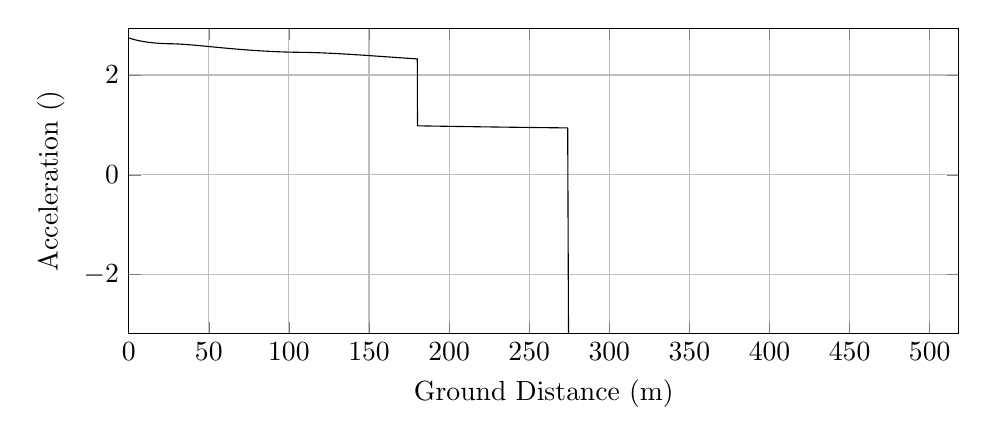
\begin{tikzpicture}

\begin{axis}[
width=\textwidth,
height=0.45\textwidth,
scaled ticks=false, tick label style={/pgf/number format/fixed},
xmin=0.0,
xmax=518.2299866992206,
xlabel={Ground Distance (m)},
xmajorgrids,
ymin=-3.1773545999999997,
ymax=2.9383329541999035,
ylabel={Acceleration ($\si{\meter\per\square\second}$)},
ymajorgrids
]

\addplot [
color=black,
solid
]
table[row sep=crcr]{
1.3729668748937997E-8	2.745933749634024\\
2.6049868369719035E-7	2.7459337463216693\\
2.0491224421327626E-6	2.7459337223163676\\
9.92442121137073E-6	2.74593361664894\\
4.7452367809869807E-5	2.7459331133935008\\
1.740064756114434E-4	2.74593141796994\\
4.0608377013922605E-4	2.7459283128250895\\
7.313431501337001E-4	2.745923966728787\\
0.0011549487327126044	2.7459183141309005\\
0.0016799013484208249	2.745911318665595\\
0.002295089346817705	2.7459031318683342\\
0.003009933382444524	2.745893631784023\\
0.003810608015426248	2.7458830054499908\\
0.004723484476856681	2.745870906509789\\
0.005727138856912631	2.7458576226878897\\
0.006836216967948795	2.7458429637322794\\
0.007997302399386296	2.7458276382144833\\
0.00929136979810952	2.745810580608766\\
0.010685558505459776	2.745792228663979\\
0.012178513621519987	2.745772603889116\\
0.013775244426719659	2.7457516442133327\\
0.015470070176169002	2.7457294279658626\\
0.0172374436815836	2.7457062929339147\\
0.019122918912604377	2.745681646264188\\
0.021104911040230538	2.7456557742244776\\
0.023190717999955576	2.7456285852738693\\
0.025355802981115103	2.7456004025085097\\
0.027620619195902148	2.7455709628304676\\
0.030020274690474198	2.7455398145480876\\
0.032476028269866286	2.7455079832228666\\
0.035054163466719815	2.745474612816359\\
0.037720846868992755	2.7454401452809734\\
0.04049779674511381	2.745404303593875\\
0.043329456594087365	2.745367807581193\\
0.04629652060163805	2.745329620662332\\
0.04934498934704602	2.745290442016606\\
0.052507657924119336	2.7452498537718295\\
0.055769483710642484	2.745208053078813\\
0.05917209570914676	2.7451645112972916\\
0.06264043916012321	2.7451201927906688\\
0.06620063977265622	2.745074766280724\\
0.06987962792775945	2.745027892179869\\
0.0736568184539585	2.744979836976057\\
0.07754284280095361	2.744930469346733\\
0.08151127871105612	2.744880128455919\\
0.08560324933017655	2.744828296550115\\
0.08985265585263943	2.7447745502252845\\
0.09413961367176535	2.7447204093860247\\
0.09857725310864562	2.744664448697618\\
0.10307959255469257	2.7446077566104368\\
0.10766008648593872	2.744550165853771\\
0.11234920964493048	2.744491296646081\\
0.11719267720457946	2.7444305805763873\\
0.12216973960582883	2.7443682839908865\\
0.12724007601918352	2.7443049160916244\\
0.13233299746505212	2.7442413617081813\\
0.13755256756750583	2.744176324555065\\
0.14287728588926696	2.744110077183268\\
0.1482946925752714	2.7440427783081276\\
0.15381585025670613	2.7439742941590106\\
0.15940564092189102	2.7439050633216198\\
0.16526271495916878	2.743832633069937\\
0.17120082448158402	2.743759314593124\\
0.17717889132867753	2.7436856165854584\\
0.18324322596131126	2.7436109697873574\\
0.189427022360885	2.7435349695339406\\
0.1957511558722988	2.743457364727397\\
0.2021484013779125	2.7433789844510024\\
0.20865863707071397	2.743299343476986\\
0.21548666343168166	2.7432159468507686\\
0.22220154781289658	2.743134061837388\\
0.22919671627301902	2.7430488935802986\\
0.23611678795738544	2.742964772871866\\
0.24306300975244904	2.7428804655838492\\
0.2503085190632165	2.7427926639555604\\
0.2576623280401219	2.74270369213178\\
0.26502430524173204	2.7426147629356477\\
0.2724963584449146	2.7425246467856903\\
0.2802001060647876	2.7424318847655185\\
0.2878583985474956	2.7423398174571867\\
0.2958320780323821	2.74224411264151\\
0.3040021452321372	2.7421462114990494\\
0.31208951788619	2.74204945948628\\
0.3202851396023423	2.7419515709453375\\
0.3287233234973125	2.7418509498073105\\
0.3370425959884752	2.7417519080250115\\
0.34575405233845447	2.7416483668644354\\
0.3545073625286812	2.7415445008529415\\
0.36338982075299686	2.74143927707345\\
0.37247557159370037	2.741331824878821\\
0.38151350442869847	2.741225116473271\\
0.3905554764834429	2.7411185361982797\\
0.3999457587520332	2.7410080342749286\\
0.4095398754587949	2.740895325049965\\
0.4189621792151833	2.7407848203234915\\
0.4285208811402964	2.7406729022160494\\
0.43828968955472236	2.7405587157868423\\
0.44807735398784176	2.740444501168418\\
0.45806002753764463	2.740328206966173\\
0.4682994371692033	2.740209125317234\\
0.4787752542918833	2.7400875051939693\\
0.4890770094685154	2.739968111629965\\
0.49985939134273727	2.739843363987376\\
0.5106597490205704	2.739718627718031\\
0.5213580865152188	2.739595283866114\\
0.532247733242454	2.739469951000051\\
0.5431365108549349	2.739344844457758\\
0.554075964429489	2.7392193713226414\\
0.5653450694020941	2.7390903409366887\\
0.5769901159382542	2.738957242270053\\
0.588512657344902	2.738825777773906\\
0.6004070039036553	2.7386903129467894\\
0.6121651247369502	2.738556638601956\\
0.6239717914322569	2.7384226491592862\\
0.6362472885961421	2.7382835883504875\\
0.6486428939173223	2.738143422272314\\
0.6610190736373547	2.7380037294208224\\
0.6737248046101814	2.7378605779440788\\
0.6862826225989949	2.7377193504710986\\
0.6991952542603428	2.7375743971928808\\
0.7122988072688032	2.737427572331951\\
0.7251463703465595	2.7372838790900627\\
0.7381769453061875	2.737138402838057\\
0.7516618647379176	2.7369881315120947\\
0.7654913705221527	2.736834310606014\\
0.7791756406994825	2.7366823919487455\\
0.7930637813125616	2.7365284991417216\\
0.8074774191984457	2.736369088689556\\
0.8215072375247947	2.7362142192435908\\
0.8361010597475598	2.736053431219534\\
0.8503303420601955	2.7358969585996338\\
0.8650627501899835	2.7357352618278403\\
0.8802332960144008	2.7355690814348668\\
0.8951742046771463	2.7354057362911055\\
0.9100334756324657	2.7352435957730297\\
0.9251067343345352	2.735079435666237\\
0.9403923630470314	2.7349132844243806\\
0.9559303815501943	2.7347447191307284\\
0.9712400158034169	2.7345789536451193\\
0.9869533781138684	2.7344091466658877\\
1.0029148609762486	2.734236997780573\\
1.0189962473881624	2.7340638988954913\\
1.035465185745812	2.733886982622522\\
1.0516742337458713	2.7337132054216866\\
1.067815735429615	2.7335404920408557\\
1.0846705971808022	2.7333605047019978\\
1.1012775250051634	2.7331835208984128\\
1.1180798406225687	2.7330048116164747\\
1.1351395900544134	2.7328237286921633\\
1.1526388687279154	2.73263835894707\\
1.1698922447507556	2.732455966615972\\
1.1875468452119025	2.732269712848928\\
1.2058383275300355	2.732077142510799\\
1.2239395537495579	2.731886975352393\\
1.2422020624207541	2.7316955142157697\\
1.2608769472440078	2.7315001426275947\\
1.2794948487006894	2.731305779649479\\
1.2979152553275424	2.7311138807814563\\
1.3166445915281573	2.73091917093961\\
1.3354141707340492	2.730724451882275\\
1.3543210821322504	2.730528719277727\\
1.373689361295591	2.73032863525778\\
1.3932049885015831	2.7301274608942405\\
1.4131781782225183	2.7299220154585475\\
1.4330139682345777	2.7297184263544425\\
1.4528243860883294	2.7295155352372795\\
1.4728783400745615	2.729310592226655\\
1.4934621752870565	2.729100693669997\\
1.5141408097620341	2.7288902940171758\\
1.53430654450827	2.7286855593626536\\
1.5553850389607948	2.728472025774905\\
1.5762653203499473	2.7282609685761434\\
1.5975496774716453	2.728046303569938\\
1.6196077215345106	2.7278243397435746\\
1.6413652536722467	2.727605899295412\\
1.663437310723463	2.7273848044555544\\
1.6860768385032747	2.727158548431424\\
1.7077101022266827	2.726942840558346\\
1.7297306410738114	2.7267237613893585\\
1.7520297891459062	2.7265024111794576\\
1.7743087535215367	2.7262817613558035\\
1.797257424336919	2.7260549980011213\\
1.8200802473615325	2.7258299974170024\\
1.8430350373473994	2.7256042147901303\\
1.8666926279964304	2.7253720605720746\\
1.8902808566018634	2.72514113040999\\
1.9138231309717848	2.7249111877288685\\
1.937187877956735	2.724683506686569\\
1.9611060682733261	2.724450973682445\\
1.9852138445648535	2.7242171481062742\\
2.009780393513653	2.723979437924413\\
2.0346228225622163	2.723739634761041\\
2.0593611988602687	2.7235014085153804\\
2.08477023517836	2.7232573149932806\\
2.110324766702745	2.7230124241566775\\
2.1352655781940433	2.722773991682768\\
2.160528860803022	2.7225330540312687\\
2.1862071157614817	2.722288750937233\\
2.2127756699400534	2.7220366021467237\\
2.2391904543957084	2.721786538650564\\
2.2653528664920257	2.721539475818613\\
2.292150575495974	2.7212870407551826\\
2.3187704640870406	2.721036905412479\\
2.3455495914188482	2.7207858982332622\\
2.372862901366455	2.7205305254301893\\
2.4007145172972395	2.7202707826704753\\
2.428100404243743	2.72001603228333\\
2.4555980306928005	2.7197608861757034\\
2.483374904362833	2.7195038000855876\\
2.511687733451976	2.7192424230947587\\
2.5402569276484597	2.7189793606402857\\
2.568415369317849	2.71872074613543\\
2.596987652715761	2.7184590025560453\\
2.6263861238451423	2.7181903927500546\\
2.655991481965028	2.717920608348247\\
2.6856115886357443	2.7176514041804687\\
2.7154221146045012	2.71738118698586\\
2.7455665152057707	2.7171086712897807\\
2.7752624694325894	2.7168409213882985\\
2.805457625653509	2.71656939071722\\
2.8358231840904597	2.716297056032584\\
2.8663460878589797	2.7160240421896784\\
2.897817297850832	2.7157433103512467\\
2.9287074004595235	2.7154685124985987\\
2.9603588456990284	2.715187708551693\\
2.9922321403815406	2.71490571640717\\
3.0241119471841866	2.71462444530067\\
3.056446055158509	2.7143399570513758\\
3.0889346922121366	2.7140549072190137\\
3.122221620829695	2.713763678408176\\
3.1546991615623394	2.7134803314856493\\
3.187635101478671	2.7131937884197734\\
3.221010117202278	2.7129042459478487\\
3.2543449374576605	2.712615872270808\\
3.288235920596943	2.7123235230382576\\
3.3223704322934555	2.7120299202652527\\
3.3562838593334394	2.7117390566035233\\
3.3906320903803255	2.7114453101597196\\
3.425633159699527	2.711146852210671\\
3.462387235801926	2.7108343880622456\\
3.4973980805087237	2.710537636483595\\
3.5324804241140235	2.710241147744873\\
3.5675385073174235	2.709945728382193\\
3.6040688981843845	2.709638816969628\\
3.6393612181513753	2.7093431890244997\\
3.6770856360342323	2.7090281416612143\\
3.7131729334920323	2.7087276833232927\\
3.749509707933214	2.7084260491268246\\
3.785733977879824	2.7081262444468592\\
3.8225309786916544	2.707822610564083\\
3.860867115351552	2.7075072478509306\\
3.89929745075254	2.7071921001654697\\
3.9373367205567504	2.706881130446619\\
3.9751626485832894	2.7065728578762025\\
4.013671158053867	2.7062599937888168\\
4.0521140617426425	2.7059486353631357\\
4.092377631210638	2.705623567578243\\
4.131586743753305	2.705308027124949\\
4.1715696979561425	2.7049872843873297\\
4.210522654700574	2.7046757949824176\\
4.250196810863292	2.704359538589963\\
4.2917015001093795	2.7040297652367293\\
4.332438976653355	2.7037071511860633\\
4.373124372895289	2.7033859958341147\\
4.414429464889761	2.703061013141131\\
4.455884944705147	2.7027359201134686\\
4.497250153511752	2.7024126010589393\\
4.537976875075978	2.7020953078843215\\
4.581399817640802	2.7017581350427298\\
4.623816269683994	2.701429893974078\\
4.666022338967499	2.7011043708260782\\
4.709098934189642	2.7007732491577343\\
4.752435367147649	2.7004412618628235\\
4.79531009100786	2.700113923220311\\
4.838191999420829	2.6997876304091646\\
4.881381760681686	2.6994601025113845\\
4.9256451804034285	2.6991255802428515\\
4.9704217340957495	2.6987883563581185\\
5.014356093293278	2.6984586198088563\\
5.058826350846283	2.698126010287651\\
5.104458009943745	2.697785910252903\\
5.149663211268795	2.697450177563721\\
5.194981168813841	2.6971147895925576\\
5.241194091283663	2.696773991377621\\
5.287987552078626	2.696430154327218\\
5.334426822383641	2.6960901499960244\\
5.380633359096258	2.6957530602096966\\
5.427524438012913	2.6954122052897027\\
5.476157635197664	2.6950599883398825\\
5.524667120325573	2.6947099813886997\\
5.5732739519824435	2.694360582160768\\
5.6208990292882195	2.6940195060851275\\
5.671502816366864	2.693658464116621\\
5.719824083529298	2.6933150154219874\\
5.767871110439133	2.6929747772519512\\
5.8169321963676754	2.6926286501345027\\
5.866076914057565	2.6922832358810025\\
5.917200682776528	2.691925289335387\\
5.96684810088939	2.6915790178532983\\
6.016885842403935	2.691231352228524\\
6.068639931677712	2.6908731577503717\\
6.119867755785197	2.6905199976544543\\
6.171030794930029	2.6901686602208663\\
6.222884713227881	2.6898139753337107\\
6.2735946138732235	2.6894684695538738\\
6.325883502103322	2.6891136013011465\\
6.379615386553551	2.6887504096481347\\
6.432194972482147	2.688396442468087\\
6.484528316464761	2.6880455368872473\\
6.536619297696934	2.68769764118571\\
6.589662958081361	2.687344796419861\\
6.644121795496577	2.6869840153423956\\
6.697445536614451	2.68663219810922\\
6.7518063163896365	2.686275003043974\\
6.8068829439682315	2.685914605406988\\
6.863205650636274	2.685547609679398\\
6.9185329265047315	2.685188625021353\\
6.974634519184049	2.684826152672259\\
7.031139830722298	2.6844626288388405\\
7.0870923879294985	2.6841041940757817\\
7.144766952910487	2.6837363176346836\\
7.2026451873548805	2.683368757231797\\
7.261191729679483	2.682998591553873\\
7.320502240843062	2.682625268876813\\
7.378210233177999	2.6822636424501294\\
7.437738452534925	2.6818922655745236\\
7.49714639104333	2.681523308417665\\
7.556502460410064	2.6811563316145213\\
7.617032771987237	2.680783794499826\\
7.676883327249088	2.6804171211405423\\
7.735740247984193	2.6800581575988813\\
7.796086087039788	2.679691776501249\\
7.856787102853412	2.6793249307229674\\
7.91721236259451	2.678961429481797\\
7.979013602666894	2.6785913752038963\\
8.039824025454376	2.6782289487607027\\
8.102419182184594	2.6778576340357727\\
8.16459313580776	2.6774905665511346\\
8.226347093952135	2.677127696565849\\
8.290527749984296	2.676752373844961\\
8.353592793320257	2.6763853613705777\\
8.417564177281012	2.67601487568339\\
8.482044607535009	2.675643270078857\\
8.547336806956285	2.6752688485572547\\
8.613293246319614	2.6748925126021685\\
8.6778048537894	2.6745262550450724\\
8.74454839911753	2.674149227258674\\
8.810708373588199	2.673777396453808\\
8.876548424968423	2.673409234250302\\
8.942828456712885	2.6730404887927257\\
9.010858044488913	2.6726639601609223\\
9.079453414959548	2.6722862922314583\\
9.148767802603732	2.6719066890561036\\
9.21609997183467	2.6715398811000908\\
9.285579683381485	2.67116336940079\\
9.355451712480097	2.670786767326205\\
9.423585014597279	2.670421494476032\\
9.493435356703696	2.6700490148237135\\
9.562655940911181	2.6696818813962357\\
9.63183713653898	2.669316926216502\\
9.703018708836247	2.6689434650398702\\
9.773178624863132	2.6685773872877823\\
9.844376937811855	2.6682079365263496\\
9.914998792594716	2.6678435040567887\\
9.98720270419701	2.6674729864037268\\
10.059478150570087	2.6671041981501142\\
10.132362020358627	2.6667344209387407\\
10.205876892438312	2.6663635857706476\\
10.279422251887688	2.6659947421935097\\
10.353305644514993	2.6656263553136483\\
10.42811398108589	2.6652555454284528\\
10.50332954727428	2.664884928557493\\
10.578207710262959	2.6645181680900603\\
10.65503529959097	2.6641441252244062\\
10.730232142651953	2.6637802356245537\\
10.805871937852555	2.6634164032193377\\
10.88265320376452	2.6630493287809767\\
10.958577899345514	2.6626885682826185\\
11.034861147941964	2.662328317504069\\
11.112742623646977	2.6619627989513033\\
11.190543636431041	2.661599949051814\\
11.267787598939979	2.6612419536263943\\
11.3462805052093	2.6608804641262784\\
11.423875697147409	2.6605253733666894\\
11.502735831556972	2.66016679186927\\
11.581465323066688	2.6598111062891867\\
11.661639233340708	2.6594512496614984\\
11.741743247575428	2.659094070532034\\
11.821864700430528	2.6587391681041073\\
11.901816327719768	2.6583873562373483\\
11.98361062800689	2.65802984404648\\
12.065425957085825	2.657674667049518\\
12.1478520915771	2.657319283720091\\
12.230956215923495	2.6569634524950505\\
12.313306905825911	2.6566132897052395\\
12.396632357805931	2.656261447402212\\
12.479578787946746	2.655913659143116\\
12.564327762802186	2.6555608318228234\\
12.648175874147956	2.655214251081233\\
12.736145481689512	2.6548532930755826\\
12.821080154398764	2.6545073614738826\\
12.908009536077355	2.6541559136608868\\
12.994986774303499	2.6538069029568296\\
13.081752199798046	2.6534613540348904\\
13.17035388279784	2.6531111740371047\\
13.257836697901475	2.652768065088189\\
13.34511613365563	2.652428366974772\\
13.433461823066896	2.6520871672573874\\
13.524108483575919	2.6517398400805456\\
13.611203924103116	2.6514087427638877\\
13.702229394080796	2.6510654420726993\\
13.792427706753081	2.650728010041674\\
13.882429934062493	2.6503940290968764\\
13.975435778888343	2.650051743756091\\
14.065832730112316	2.6497218173613817\\
14.157894546480026	2.649388598244756\\
14.250668806951023	2.649055631782466\\
14.343291987615704	2.6487260325270725\\
14.43744444968501	2.64839387373258\\
14.532636396723657	2.6480609912501123\\
14.625507232812737	2.6477390675021404\\
14.721503924398366	2.6474092478024884\\
14.818738382089133	2.6470782104461428\\
14.913572076739943	2.6467582780736505\\
15.009701633366973	2.6464369177531655\\
15.10815424447124	2.6461108524555685\\
15.206130868840724	2.6457894275225193\\
15.304035939715973	2.6454712794394446\\
15.403499839366233	2.645151168619309\\
15.503209871950865	2.6448333932172794\\
15.601718454553605	2.6445225108434887\\
15.700655560608023	2.6442133305209685\\
15.801250929860519	2.6439020954003567\\
15.899917805652187	2.643599879299895\\
16.001574124100856	2.6432916569963822\\
16.102638779863817	2.6429883870635598\\
16.204479333764816	2.6426859631921458\\
16.30489644092564	2.642390875444015\\
16.40578186591999	2.6420975095348966\\
16.509201471948074	2.641799986524223\\
16.614557195984908	2.6415002256988815\\
16.717657554831042	2.641210126302675\\
16.823039336622365	2.640916912552081\\
16.928576062495388	2.6406266046044653\\
17.03469945574068	2.640338038396731\\
17.140697318244236	2.640053160739731\\
17.246066414787876	2.639773277049187\\
17.35183930840021	2.639495622702711\\
17.458399953804133	2.639219234411631\\
17.565707112453843	2.6389442799060117\\
17.673103795073075	2.638672470550473\\
17.781888038667653	2.638400579402105\\
17.89115167195854	2.6381309531423165\\
18.00105710767307	2.63786323255278\\
18.110142905530395	2.6376009574466197\\
18.219697237410173	2.637341002414172\\
18.32752951944549	2.6370884953076636\\
18.43743745973078	2.6368345484445737\\
18.54904630654982	2.63658019384358\\
18.659302591714813	2.6363323952736817\\
18.770734536087716	2.636085450694776\\
18.883577445650936	2.635838949357387\\
18.996263390583444	2.635596364184675\\
19.108816920034535	2.635357616908477\\
19.22287647779894	2.6351192855805\\
19.33763586704334	2.6348831480062795\\
19.456324114791514	2.6346427711361047\\
19.57349394116079	2.634409291852097\\
19.690148252848566	2.634180600096859\\
19.80521137071168	2.633958691418372\\
19.92379170801214	2.633733794227746\\
20.04216631061405	2.6335131166802155\\
20.15848954929409	2.6332999786096893\\
20.278242138037896	2.6330843918964613\\
20.396206084226087	2.6328758170334643\\
20.516315546862906	2.632667302876359\\
20.637173924977112	2.632461401533406\\
20.75450010628387	2.6322652607421713\\
20.874378237858778	2.632068650375719\\
20.996035953832852	2.6318730325170687\\
21.11812959618858	2.6316806625120934\\
21.240471115580952	2.631491857446668\\
21.361479376438375	2.6313089928781865\\
21.485224699488654	2.631125973433857\\
21.607870280890317	2.6309485406063304\\
21.73242999733349	2.630772361329301\\
21.85704493170313	2.6306001480967662\\
21.98122016226351	2.6304325538620574\\
22.10826921766411	2.6302652125995127\\
22.235261614051304	2.6301021093246337\\
22.361664688868032	2.629943883831288\\
22.48780138980522	2.6297900776934346\\
22.614107216476143	2.6296401428980527\\
22.74409311379692	2.6294900871360998\\
22.873024137794893	2.6293454925824022\\
23.003512644166257	2.6292034414201826\\
23.132891545907036	2.629066846405708\\
23.26270690888247	2.628934029456868\\
23.39264146728729	2.6288053298831127\\
23.52277721573431	2.6286806696961964\\
23.654883767164463	2.6285584477188975\\
23.78569183677709	2.6284417091087624\\
23.917003007077597	2.628328794588147\\
24.047013652206026	2.628221204195908\\
24.178458227988493	2.6281166694027984\\
24.314609552493202	2.6280128759318746\\
24.447533097503474	2.627915932898171\\
24.579128452041708	2.627824218719879\\
24.71011994849615	2.627737123338611\\
24.843278471916108	2.627652868038229\\
24.975761222328053	2.6275733117861915\\
25.1115496753864	2.6274961796102385\\
25.247101122854083	2.627423621584068\\
25.384906965000688	2.627354391118195\\
25.522261036073317	2.6272899242628656\\
25.66123001648475	2.627229296090176\\
25.79865327455613	2.627173876444852\\
25.826335196219034	2.6271632574604533\\
25.839610403727477	2.62715822969495\\
25.841006316401874	2.627157703174394\\
25.84227013303559	2.6271572259940434\\
25.84770509053729	2.6271551682557828\\
25.86419328224909	2.627148869514051\\
25.90571916957557	2.627132632727095\\
25.999268866927544	2.62709410603191\\
26.123295978662824	2.627038901212371\\
26.250212562581652	2.6269775933396176\\
26.376891976518465	2.626911599588503\\
26.50638698165423	2.6268392423555404\\
26.634042370994827	2.6267631265942892\\
26.763333806613538	2.626681250837172\\
26.893207366259766	2.62659421847878\\
27.022905486492228	2.6265025738361114\\
27.153956322362554	2.626405232066988\\
27.287774297957696	2.626300978647955\\
27.42030033806219	2.6261929566003683\\
27.555504894698295	2.626077916748084\\
27.691130018821354	2.6259576762016144\\
27.82633313037239	2.6258330443348266\\
27.959508564917073	2.625705689812035\\
28.096515548835796	2.6255699768647354\\
28.232789703382153	2.6254303281033025\\
28.368684388406535	2.625286498680893\\
28.506541650227618	2.6251359904785243\\
28.64533374691623	2.624979841336361\\
28.78297783415192	2.624820465669056\\
28.92277775692753	2.6246540493487274\\
29.06227187463503	2.624483493060775\\
29.20212864139956	2.6243080372215513\\
29.34335827861657	2.624126392094661\\
29.483225747293005	2.623942134485322\\
29.625960812476485	2.623749682168036\\
29.76706561118049	2.6235551018597727\\
29.909402910999468	2.6233545237810842\\
30.051751399473822	2.623149671618658\\
30.196612335666572	2.6229368923312792\\
30.342192969749448	2.6227187353115538\\
30.48583400527584	2.6224992991267593\\
30.632658550781265	2.622270763203243\\
30.77846394498075	2.6220396350772806\\
30.92408133049836	2.6218047080288107\\
31.071091331299215	2.6215634400823893\\
31.218274793935116	2.6213178254024356\\
31.366705758252415	2.6210660719563164\\
31.515339333797037	2.6208099515408767\\
31.66356819769615	2.620550577189582\\
31.814689402684216	2.6202821391202162\\
31.96649953392354	2.6200084685109024\\
32.115424616034375	2.6197361526902787\\
32.266253234088566	2.619456531320976\\
32.41813832080348	2.6191711196609058\\
32.569791431087395	2.6188823653016966\\
32.722234201183724	2.618588359660447\\
32.876984607664	2.6182861188418736\\
33.031873994672836	2.6179798472058744\\
33.18502245018544	2.61767337730517\\
33.34135780547538	2.6173568541876238\\
33.49759920343199	2.6170368690402794\\
33.65385117142162	2.6167132684054444\\
33.8113313806527	2.6163835453824538\\
33.96985264489639	2.6160480723691215\\
34.126473036379195	2.6157131607910555\\
34.2857505660089	2.6153690959358693\\
34.4449212019973	2.6150218218705428\\
34.60566879064274	2.6146676745052684\\
34.76644486933921	2.614310071010496\\
34.92612701881755	2.613951597544056\\
35.08630421658309	2.6135887608266746\\
35.24825698849928	2.613218646437778\\
35.412303951281956	2.6128404656979436\\
35.57355277914179	2.612465573208352\\
35.73545353069308	2.612086065190393\\
35.89925038949356	2.6116990063305368\\
36.065161289279985	2.611303822719635\\
36.23047312008262	2.6109069894047563\\
36.39472205714358	2.6105097203642957\\
36.56135389445764	2.6101036997752756\\
36.72774532558607	2.609695316287241\\
36.89384825683493	2.6092847556652456\\
37.05904296416534	2.608873633171015\\
37.22702676294645	2.6084527521107095\\
37.39437475321985	2.6080306918927274\\
37.5621109943643	2.607604928234461\\
37.73270471709142	2.607169167240153\\
37.903359519601935	2.6067305347705387\\
38.071486842086316	2.6062957943756917\\
38.23815243703595	2.6058623319798837\\
38.40817787072022	2.6054176148453294\\
38.57751392140098	2.604972224462812\\
38.750215798728505	2.604515486819169\\
38.92001182640311	2.604064028086343\\
39.09310637700479	2.6036013939253158\\
39.26472366117933	2.603140360230884\\
39.436554723976656	2.6026764590104268\\
39.608961777617054	2.602208745072529\\
39.782828308010565	2.6017348303452126\\
39.956194359016465	2.6012600869258415\\
40.132391837044906	2.6007753954833523\\
40.30868053167249	2.6002882883371417\\
40.48611580488176	2.599795875967091\\
40.66383502946924	2.599300575623608\\
40.83999042132467	2.5988076076289266\\
41.018202681018664	2.598306879012876\\
41.19780999006247	2.59780023921822\\
41.37730467548502	2.5972919679986406\\
41.557010452813884	2.5967811949022925\\
41.73612816026986	2.5962702442991796\\
41.91555194917056	2.5957566162813004\\
42.09743589423803	2.5952341495078093\\
42.27807550146298	2.5947135135520316\\
42.45995188234755	2.594187603754664\\
42.6401410478328	2.593664926422731\\
42.822293873795985	2.5931349327029034\\
43.00585672428667	2.5925992336587598\\
43.189965171449515	2.592060371841985\\
43.372020236704074	2.5915260176090396\\
43.555636897252796	2.5909856106444664\\
43.74012033961118	2.5904412105939336\\
43.92429822300048	2.5898963139394615\\
44.106869824379004	2.5893548329369107\\
44.29411840239129	2.588798141810776\\
44.47920670866131	2.5882465834656143\\
44.665034305215386	2.5876915745572395\\
44.85242224248053	2.5871306821366113\\
45.03948098831597	2.5865695920897522\\
45.22811764277584	2.586002614453135\\
45.41548629589063	2.5854383417605273\\
45.60322541388645	2.58487188864763\\
45.793007222766036	2.584298230300096\\
45.983742663331824	2.583720675421648\\
46.172643153142886	2.58314771556424\\
46.36421599110457	2.582565713945945\\
46.553512793459404	2.5819897407332553\\
46.745018895697555	2.5814061887802406\\
46.93606459490553	2.580823220829023\\
47.126948089509526	2.580239969889381\\
47.31881294044018	2.579652975509168\\
47.5110690178297	2.5790640736859434\\
47.705448624448266	2.5784679831468953\\
47.90005519882567	2.577870546429364\\
48.09288923506665	2.577277947636331\\
48.28732881729917	2.576679844114947\\
48.484002572746206	2.5760743233998253\\
48.68089030454945	2.575467633349363\\
48.87532723390382	2.57486803095897\\
49.07073736177763	2.5742649991859343\\
49.2672083392297	2.5736582972862303\\
49.46586249263092	2.5730444865995894\\
49.661880987188695	2.5724384938105347\\
49.85966148345089	2.5718267615262587\\
50.05808618672894	2.571212777407524\\
50.25785665917266	2.570594402569249\\
50.45743808511885	2.569976421527972\\
50.65573800086891	2.5693622538365988\\
50.85948768734909	2.5687310825359084\\
51.061243703011925	2.5681059980424292\\
51.26368286286315	2.567478743109982\\
51.46416466063809	2.566857533975103\\
51.66475943174029	2.5662359893110347\\
51.86588207153103	2.56561285677663\\
52.07444928962187	2.564966744465173\\
52.2824430085781	2.5643225310284814\\
52.48676525705545	2.5636898422625745\\
52.69531994892206	2.5630442386830037\\
52.90027076850366	2.562410012697458\\
53.108186167814935	2.5617668705752035\\
53.31165724918766	2.561137759462768\\
53.520024946679996	2.560493831718171\\
53.72688450142306	2.559854920280424\\
53.93707391647578	2.5592061198138465\\
54.14518573319289	2.5585641573342945\\
54.35125853722778	2.5579289322446064\\
54.56213447502874	2.5572793940255876\\
54.77598621923464	2.5566212311207\\
54.987629956235494	2.5559704324655836\\
55.19778857845695	2.5553247914147734\\
55.41030974885841	2.55467252202679\\
55.62390503323701	2.554017625167454\\
55.83671574169797	2.553365831759879\\
56.047071254351536	2.5527222723040826\\
56.26137331252919	2.5520673989185383\\
56.47512769358855	2.5514149930840677\\
56.69105800830218	2.55075678108659\\
56.90937011004422	2.5500921924420785\\
57.12736617899088	2.549429482767894\\
57.346833156368504	2.5487632574065238\\
57.56476609337061	2.5481026676419045\\
57.78230894703917	2.547444262133678\\
57.99943865551505	2.5467881336539273\\
58.21827465292657	2.5461279153126446\\
58.436085045729726	2.545471882108224\\
58.6577546799423	2.5448053710641405\\
58.87982836766625	2.544138832936956\\
59.10336118170943	2.5434691447546607\\
59.324182403931715	2.542808819305696\\
59.545440661451366	2.5421484495030766\\
59.768227251413464	2.5414848224466517\\
59.99077485409802	2.540823240966116\\
60.21631063559073	2.54015416369662\\
60.44006004384342	2.539491792913134\\
60.66502706168687	2.5388272572727564\\
60.89133011288284	2.5381602583073883\\
61.11585558357916	2.5374999948556693\\
61.3432655409558	2.5368327945800493\\
61.57186440401435	2.5361637002878803\\
61.79868765088207	2.535501408748763\\
62.025670725987	2.5348402770909786\\
62.254132946411545	2.5341765056009926\\
62.48290793247415	2.5335135279774255\\
62.713817944074236	2.5328461162466924\\
62.94484116346062	2.5321801651283318\\
63.17805109236767	2.5315097497788024\\
63.41124119062552	2.530841264404774\\
63.64505576847972	2.5301728944345925\\
63.87735201907903	2.5295107788661895\\
64.11169045660182	2.5288448001638137\\
64.34725756208485	2.52817733598523\\
64.58324360279937	2.527510726208688\\
64.81881329818131	2.5268473544899654\\
65.05563560606473	2.5261825559991893\\
65.29467812810154	2.5255136850947695\\
65.53178653633495	2.524852393698131\\
65.77046761369158	2.5241889200770515\\
66.01019347650049	2.523524791474693\\
66.25262920761091	2.52285547188822\\
66.49342175078831	2.522193018006006\\
66.73393309567928	2.5215336779391944\\
66.97718905970893	2.52086921586132\\
67.21919788222482	2.5202105803525665\\
67.46413738735515	2.519546449583455\\
67.70584739194695	2.518893544044623\\
67.95375887035246	2.5182264574902717\\
68.19817148521656	2.5175713561374016\\
68.44413350233111	2.5169147004876002\\
68.68984243621705	2.516261345089669\\
68.93951041285982	2.515600171501796\\
69.19023531750676	2.514938969433662\\
69.43956667494601	2.514284217583624\\
69.68998597860525	2.513629416130965\\
69.94098943220166	2.512975932155717\\
70.1928405184459	2.5123231255440013\\
70.44659484061637	2.511668329081634\\
70.69926103579675	2.5110192971929557\\
70.95414956377036	2.5103675673854084\\
71.21136313866151	2.5097129793716446\\
71.46778788208749	2.509063506597747\\
71.7247351381395	2.5084158438377147\\
71.98234155897126	2.507769689085089\\
72.24107377350035	2.5071239256193767\\
72.4986091150376	2.5064843695454924\\
72.75949164810788	2.505839797213234\\
73.02014691132015	2.505199119753618\\
73.28114866838587	2.504560949336046\\
73.54342372888959	2.503923071226774\\
73.80584407854005	2.5032882764078206\\
74.07231166191039	2.5026472290607487\\
74.3389341302921	2.5020093971959803\\
74.60521354141642	2.501375988177486\\
74.87280568706873	2.5007431028336446\\
75.1403821105715	2.5001139292433843\\
75.41145333671997	2.4994803046180856\\
75.68265298797411	2.4988501932497016\\
75.95075857762194	2.498231039158717\\
76.2241428819712	2.4976035721719434\\
76.4990100438061	2.496976668570306\\
76.77213586328236	2.4963576955699853\\
77.04724851790667	2.49573822862106\\
77.32330034006353	2.4951207098630084\\
77.59850473375684	2.4945091566067346\\
77.87773830129439	2.4938928219842715\\
78.1565255546137	2.4932816837060106\\
78.43842651648492	2.492668017346257\\
78.720833678605	2.4920576010425153\\
79.00101298089581	2.4914563231480757\\
79.28359351218376	2.4908542717934887\\
79.57011733099088	2.490248328576058\\
79.85418914588558	2.4896520718283295\\
80.13919871477489	2.4890583687052414\\
80.42568449319114	2.4884661731421938\\
80.71472498530085	2.487873370981382\\
81.006853148924	2.487279025102887\\
81.2951972638476	2.4866971170884167\\
81.58524575795963	2.486116537145639\\
81.87461709596036	2.4855420949920353\\
82.1711642895769	2.484958381559892\\
82.46716486408064	2.484380782761332\\
82.76422974563803	2.483806186216814\\
83.05801377197795	2.483242957146957\\
83.35853301954708	2.482671999870737\\
83.65664966506407	2.4821108049392793\\
83.95487262936624	2.481554606519677\\
84.25322789115987	2.4810033792257986\\
84.55664509033022	2.4804481694309706\\
84.8599544590121	2.4798985860092557\\
85.16499148084048	2.4793513638033664\\
85.47187188044902	2.478806409028219\\
85.77908321853027	2.4782664837735044\\
86.08675489504844	2.4777313991684684\\
86.39784539041122	2.4771961342162765\\
86.71051296037359	2.4766640142286205\\
87.02583358957506	2.4761333445033173\\
87.34037846285594	2.4756099658506825\\
87.65395388450591	2.4750941674588303\\
87.96687312379424	2.4745854039580317\\
88.28527441497255	2.474073850456792\\
88.6103524516937	2.4735579588692937\\
88.92871226770333	2.4730590021066936\\
89.25003295857354	2.472561715850354\\
89.57522243846881	2.472064913921284\\
89.90247582737899	2.4715715482953424\\
90.22602529632545	2.471090281458441\\
90.5494223037065	2.4706157304863785\\
90.87816525326718	2.470140000358535\\
91.20455861430293	2.4696743344984124\\
91.53817773235312	2.4692052383281\\
91.87076195087604	2.46874453523425\\
92.20124984301029	2.468293613714687\\
92.53140503523474	2.4678500072923946\\
92.86389705561814	2.467410207209607\\
93.19815266874983	2.46697511608851\\
93.53304529783748	2.4665462917878456\\
93.86737084100128	2.4661252936021194\\
94.20337949361911	2.4657093387407842\\
94.54065981474497	2.4652990463300517\\
94.87396787418089	2.4649007234996034\\
95.21684847579547	2.4644983797555815\\
95.55392648231228	2.4641101935898275\\
95.89232371872416	2.463727831543161\\
96.23051075783204	2.463353072193108\\
96.57164052232307	2.4629825255521096\\
96.90762523479154	2.4626249186321765\\
97.24755293575913	2.462270552927021\\
97.58790661409188	2.4619232523826478\\
97.92576087813703	2.461585947168559\\
98.26661027452474	2.4612531815923795\\
98.6051908024865	2.4609301321117414\\
98.94563962387357	2.4606128512157275\\
99.28665364663627	2.4603026475156407\\
99.63350087797645	2.4599949576702347\\
99.97685593767679	2.4596981466115277\\
100.31593955776762	2.4594126383431973\\
100.65572384630482	2.4591341387793317\\
100.99616871909686	2.4588627388350837\\
101.3402339503516	2.458596236175948\\
101.67973054404297	2.458340953841132\\
102.01657591573795	2.4580952179760907\\
102.35656456518868	2.457854829697289\\
102.6941824316649	2.457623725275984\\
103.03547296258705	2.457397823628013\\
103.37623032340073	2.457180026797986\\
103.71852978299776	2.456969054425172\\
104.05851119314701	2.4567672705298635\\
104.3949509202441	2.4565752126830196\\
104.7329053851843	2.456389936423986\\
105.07104272194636	2.456212240406991\\
105.40742307340048	2.456043101164078\\
105.74423560014887	2.4558813834138933\\
106.07955743077031	2.455727984822288\\
106.41623710643992	2.4555816081016255\\
106.75618472497374	2.455441591416804\\
107.0942647435474	2.4553101084432747\\
107.43151869252583	2.4551866717490167\\
107.44650965670576	2.4551813642403237\\
107.45815118347005	2.4551772531208176\\
107.46233674961977	2.4551757772689795\\
107.46535588765028	2.4551747132015054\\
107.46808502617694	2.4551737507643727\\
107.4836206108138	2.455168259670489\\
107.53176708907421	2.4551511079163477\\
107.68672244793561	2.455094531599669\\
107.97570433527497	2.4549834451948627\\
108.27744765146667	2.4548597682328195\\
108.5816623935838	2.4547272061477434\\
108.88557241638279	2.4545869610121596\\
109.19209959959528	2.45443767243568\\
109.50241879336687	2.4542786003150896\\
109.81066605766154	2.4541127633367736\\
110.12101503747155	2.453937994054648\\
110.43285681965125	2.4537545790192175\\
110.74725799716322	2.453561818956234\\
111.06462449033057	2.4533593397004765\\
111.38211128519615	2.453148923592198\\
111.70119562731901	2.4529296108117045\\
112.02298633508096	2.452700564309909\\
112.34320819983824	2.452464869014065\\
112.66812620709393	2.452217884637398\\
112.99302416686388	2.451963112159949\\
113.31966045518399	2.4516991968576756\\
113.64998129974768	2.451424459279832\\
113.97857627498675	2.451143416865058\\
114.31304608469316	2.450849510906499\\
114.64448318111735	2.4505505571921855\\
114.98093514978115	2.4502393175308965\\
115.31969924418831	2.4499181287839766\\
115.65790718621022	2.449589741128423\\
116.00063352526521	2.4492491841404753\\
116.34235083463872	2.448901923487149\\
116.68621873349733	2.448544803075687\\
117.03331062078092	2.4481766222286128\\
117.37910048629482	2.4478022122028253\\
117.72869476105836	2.447416056567934\\
118.08005947084649	2.447020315368726\\
118.43363644355449	2.44661445841039\\
118.79186464668504	2.446195562722882\\
119.14769212941735	2.4457719010897243\\
119.5036618261702	2.4453406161077478\\
119.86270697471275	2.444898151431988\\
120.22616362054572	2.4444427272159954\\
120.58991121293201	2.4439794620158324\\
120.95538130513773	2.443506572675182\\
121.3195355377388	2.4430280793612997\\
121.68590041554987	2.4425394226513815\\
122.05305648207542	2.442042507730611\\
122.42257239354896	2.4415352206266228\\
122.79503144936103	2.4410167087569397\\
123.16629137010841	2.4404927909789507\\
123.53950748252527	2.439959095724661\\
123.91239367862553	2.4394189483888704\\
124.29026003316017	2.4388646308631676\\
124.66301933937496	2.438311045841078\\
125.03890311735066	2.4377461242287524\\
125.41380975776434	2.4371760734767376\\
125.7896808967325	2.4365980418067945\\
126.16837244152023	2.4360091772577572\\
126.54595968852882	2.4354156387065453\\
126.92471834906405	2.434813947054397\\
127.30294276405039	2.4342068948637348\\
127.68255852126984	2.433591469128208\\
128.06243727540487	2.4329695571547303\\
128.44360431740483	2.432339541404442\\
128.82265748788262	2.4317071612453454\\
129.1989690567886	2.4310736703116387\\
129.57765386613931	2.4304305602421765\\
129.95508099647026	2.429784065084977\\
130.33359114840187	2.4291302715149827\\
130.71373745886524	2.4284682576146626\\
131.09453904397424	2.4277997749107643\\
131.47657586018488	2.4271238577704235\\
131.85678563989967	2.426446027201812\\
132.23856625352113	2.42576032125654\\
132.61595336405918	2.4250775964184523\\
132.99976263915818	2.4243783357290276\\
133.38083522978053	2.423679242984316\\
133.76098428781995	2.4229771481541835\\
134.1363519425165	2.4222793654313444\\
134.51557915495124	2.421569932295995\\
134.8968696170101	2.4208521881638854\\
135.27419431482667	2.420137597883574\\
135.65215477207505	2.4194175854598914\\
136.03329358991255	2.4186873250908105\\
136.41192880753374	2.4179577730609862\\
136.7898079310749	2.417225694571063\\
137.17001317148595	2.4164851729427035\\
137.54844558779996	2.415744261492118\\
137.92617219433072	2.4150009862160164\\
138.30476964659732	2.4142523189260237\\
138.68390038934075	2.413498983015482\\
139.0631653430654	2.4127418378009757\\
139.4406106933401	2.41198488197385\\
139.81914660512416	2.4112223633220573\\
140.19767098864742	2.410456560906317\\
140.5730919292459	2.4096938425620706\\
140.95061983253072	2.4089237067743268\\
141.32838502869612	2.4081500093041033\\
141.70636515873298	2.4073728610224387\\
142.0839785067887	2.406593529688587\\
142.46357402350594	2.4058072184921997\\
142.84082211769783	2.40502296889394\\
143.21906727224075	2.4042339114596416\\
143.59963619096823	2.403437310882776\\
143.97984478872678	2.4026388326905357\\
144.35941603837455	2.4018391364099507\\
144.7355521893594	2.4010442230400466\\
145.11296635073694	2.4002442180265584\\
145.49073213867456	2.399441133914113\\
145.87033631970945	2.3986318541955978\\
146.24486520181193	2.397831210000894\\
146.6238757206513	2.3970188391759493\\
147.00096360401335	2.396208508945593\\
147.37874202190085	2.3953946757121454\\
147.756852900845	2.39457816388311\\
148.13572640408995	2.393758097000817\\
148.5136798644104	2.392938178662493\\
148.89083780486442	2.392118210713834\\
149.2712459042852	2.391289439886328\\
149.65303236723025	2.390455972301191\\
150.0329584616291	2.389624940771009\\
150.41363382646614	2.388790702960881\\
150.79322940570728	2.3879573271300165\\
151.17272478467066	2.3871227269328097\\
151.55400296227282	2.3862828087520374\\
151.93482601265913	2.385442551958211\\
152.31881414221942	2.3845940116132027\\
152.70208150063132	2.3837458190581575\\
153.08320649997165	2.382901190023449\\
153.4666285558243	2.382050340959543\\
153.84825937276264	2.381202396702336\\
154.23093781718723	2.380351107148919\\
154.61485031834388	2.379496102763693\\
155.00001234931443	2.3786373939872023\\
155.38285725409855	2.3777829898524283\\
155.7679513537659	2.3769227531344317\\
156.1509667875323	2.3760664034774726\\
156.53491934392343	2.3752072536116557\\
156.91995289130983	2.37434502792717\\
157.30625057946366	2.373479362158138\\
157.69121706207227	2.3726161237217385\\
158.07789765133754	2.371748534188164\\
158.46521012398495	2.3708790680405922\\
158.85138765236047	2.370011742814021\\
159.23964669847322	2.3691393833615075\\
159.62715395386465	2.368268403666744\\
160.01960115328984	2.367386056204964\\
160.4079207075476	2.366512776596168\\
160.79602490671402	2.36563981902208\\
161.18437278725975	2.364766199221803\\
161.57644284003254	2.363884138972799\\
161.96812230097612	2.363002938647095\\
162.35808768568592	2.362125623778489\\
162.75087300343483	2.3612420420191382\\
163.14546270495134	2.3603545272165904\\
163.53745675514648	2.3594730228399685\\
163.92955389373896	2.3585915050473067\\
164.32395276810763	2.357705079439211\\
164.71713266653478	2.3568217061873185\\
165.1102153740033	2.35593890902884\\
165.5035884424101	2.355055863096327\\
165.89816400198282	2.3541705682312966\\
166.29148626774366	2.3532885788431104\\
166.68861804276264	2.3523985917182593\\
167.082852347146	2.351515683455717\\
167.48006204110857	2.3506267458495653\\
167.8798182678497	2.349732796398407\\
168.27774435731556	2.3488436682392644\\
168.67741362640317	2.3479514207768712\\
169.07475368467374	2.3470651868695898\\
169.4759958044982	2.3461711163376826\\
169.87832784425882	2.3452755349517966\\
170.2792240364854	2.344384106753197\\
170.68126852540456	2.3434911272918937\\
171.08617821288442	2.3425928410644596\\
171.48766933901368	2.341703228415432\\
171.892744970828	2.340806814987485\\
172.29711201372032	2.339913155185136\\
172.70264003426053	2.339018160916506\\
173.1105289448074	2.3381192418897934\\
173.5163733808056	2.337226149563117\\
173.92577914808027	2.336326596791209\\
174.33607303977334	2.335426521117654\\
174.74614233406845	2.3345284082190787\\
175.15731444736514	2.3336293965914052\\
175.56901623635082	2.3327307892227083\\
175.97955109701695	2.3318363258755\\
176.39275298155184	2.330937702273025\\
176.80397138375372	2.3300450760546294\\
177.21946344336607	2.329144919042588\\
177.6332252263685	2.3282502942964154\\
178.05102033212842	2.3273487947563245\\
178.46725124888752	2.3264525543676644\\
178.88389799206544	2.325557341115923\\
179.29839533747668	2.324668693141324\\
179.71608569665375	2.3237752025766305\\
180.1342696339205	2.32288270874726\\
180.26454521656194	0.9819097825897585\\
180.5538779958007	0.9815536538867426\\
180.97677279803082	0.9813338843741317\\
181.73177043104909	0.9809420613829676\\
182.61825861954026	0.9804828804582393\\
183.4994266290775	0.9800274114937022\\
184.38832398643513	0.9795689259516667\\
185.2752206450968	0.9791124645948044\\
186.16090254585617	0.9786576300079914\\
187.05782443666988	0.9781980558527161\\
187.95004436743	0.9777419344260561\\
188.84343565256296	0.9772862693797477\\
189.73203483232732	0.9768341080623215\\
190.63087969896367	0.9763778205536682\\
191.53167348748025	0.975921653048007\\
192.42914206966827	0.975468285978192\\
193.32936064878362	0.9750146613483333\\
194.23353734669462	0.974560195085505\\
195.14873951553636	0.9741013759586223\\
196.05846844349168	0.973646498220359\\
196.9665797060448	0.9731936319952481\\
197.88137813217617	0.9727386577834067\\
198.80153314772656	0.9722822736673473\\
199.72262566550114	0.9718266963438293\\
200.6418018332526	0.9713733471887152\\
201.57021605131746	0.9709167520076665\\
202.49227039761405	0.9704645997371386\\
203.4093310979173	0.9700162077043244\\
204.33741716634955	0.9695637680397735\\
205.26228808295895	0.9691142513984239\\
206.1977933698634	0.968660954442008\\
207.13719708861407	0.9682071851823584\\
208.07111616454222	0.9677574839439917\\
209.00693662932974	0.9673082974336158\\
209.95866810149408	0.9668529538553194\\
210.9046028778589	0.966401874140419\\
211.84706310840727	0.9659539404415134\\
212.79298368779843	0.9655058679602557\\
213.73594859980489	0.9650607082011593\\
214.69266347370274	0.9646106120376037\\
215.65468447394903	0.9641596099968146\\
216.614658409948	0.9637111687218229\\
217.57357224144454	0.9632648305908005\\
218.5368107467741	0.962818108565535\\
219.50048157907025	0.9623728309632855\\
220.46765259916174	0.9619276013775406\\
221.44618219131166	0.9614788520305291\\
222.41939214233116	0.9610342584103961\\
223.3957502333693	0.9605899574694503\\
224.37068692464283	0.9601480441284298\\
225.34711146005128	0.9597072107126363\\
226.33138885023874	0.9592646196979733\\
227.31393394086427	0.9588246086557728\\
228.30414603792985	0.9583829955386565\\
229.29617452368518	0.9579424268093641\\
230.2808212657469	0.9575069825076572\\
231.28192033792595	0.9570661588058118\\
232.2770741096358	0.9566298588307522\\
233.29052711380916	0.95618749978573\\
234.30070953924962	0.9557485512780175\\
235.3030940983469	0.955314958700952\\
236.31056730234104	0.9548811504446497\\
237.32863543123972	0.9544448128053211\\
238.35192702989485	0.9540083062755578\\
239.37227626200922	0.9535751317788841\\
240.40154009491766	0.9531402846341996\\
241.4327935450462	0.9527067349006038\\
242.46479014370783	0.9522750257935997\\
243.4993601598722	0.9518444126890224\\
244.5489899152056	0.951409765141009\\
245.59198540953986	0.9509801041802433\\
246.64178332136828	0.9505499058577891\\
247.69238009267121	0.9501216656846319\\
248.75653132082437	0.9496902421588573\\
249.80604502438968	0.9492670717559109\\
250.8683150903493	0.94884111346347\\
251.93058205288185	0.9484175367509002\\
253.00701197053712	0.947990751489465\\
254.08005928692728	0.9475677615536788\\
255.1482320588113	0.947149137302701\\
256.2287194565513	0.9467281783690769\\
257.30711015243367	0.9463105453147493\\
258.39583303573465	0.945891464178104\\
259.47850143980736	0.9454772681717731\\
260.57344571603574	0.9450609772977574\\
261.6820544046054	0.9446421674171024\\
262.77228099849674	0.9442329385071817\\
263.87126070008526	0.9438230805580119\\
264.97335243767543	0.9434147508720228\\
266.0976894214622	0.9430009646912096\\
267.21278411159847	0.9425933692474135\\
268.32534355771804	0.9421894793154701\\
269.4561922169971	0.9417818049896611\\
270.5915896156504	0.9413753973257679\\
271.7158392961418	0.9409758600137457\\
272.8552569839427	0.9405738670325356\\
274.01601268837805	0.9401673947556581\\
274.6537304893817	-4.176886718010094\\
275.14755464888765	-4.176263446656387\\
275.85830180021594	-4.180251418550371\\
276.56759366538427	-4.184235021374995\\
277.278077811407	-4.188229126202462\\
277.9895493380078	-4.192232602321321\\
278.6927642223736	-4.196193378514863\\
279.3910306206568	-4.200129985618753\\
280.0942588944238	-4.204098298766938\\
280.79641638373937	-4.20806431021464\\
281.4975379179365	-4.212028203384714\\
282.193286517149	-4.215965410950371\\
282.8910199818474	-4.219917546858905\\
283.5865968378763	-4.223861154853406\\
284.27433156418897	-4.227763924785576\\
284.96299716256124	-4.231675590661785\\
285.6501548972243	-4.235582299094219\\
286.33962115543466	-4.239505757107137\\
287.02583094263616	-4.243414292555691\\
287.71598279024295	-4.247348915836691\\
288.39552192914357	-4.251226599591256\\
289.07064069118167	-4.255082564873888\\
289.75084138147497	-4.258971092825226\\
290.43056417888477	-4.262860438594373\\
291.10380028445877	-4.266716168888653\\
291.7762514232942	-4.270570884938923\\
292.44909533643477	-4.274431338055196\\
293.1182529402639	-4.27827410199898\\
293.79026574103943	-4.282136739287335\\
294.45906539508985	-4.285984370252587\\
295.12196486259893	-4.289801468800546\\
295.7884879959788	-4.293642860530859\\
296.44464661152506	-4.297427878159768\\
297.09971932539725	-4.3012099601842735\\
297.75574809817397	-4.305000897871695\\
298.410414739628	-4.308787295127042\\
299.05495102812733	-4.312518354784341\\
299.7034521878037	-4.316275626763783\\
300.35736267283187	-4.32006755376999\\
301.00367759475023	-4.323818708714663\\
301.64168722415786	-4.327524855109246\\
302.2794405972901	-4.331232687728519\\
302.91547972896694	-4.334933718003153\\
303.54547534360563	-4.3386026994092095\\
304.174491838211	-4.342269076694691\\
304.8074045744022	-4.3459612913411\\
305.43683326410905	-4.349636294747064\\
306.06248329297875	-4.353292315636455\\
306.6837108687629	-4.35692553417522\\
307.3022088341245	-4.360545801015306\\
307.91370868576485	-4.364128062941992\\
308.53029041852244	-4.367743075006773\\
309.141747702943	-4.371330999735848\\
309.7569417648659	-4.374943825637104\\
310.3587552160037	-4.378480960960191\\
310.9608346900111	-4.382022521487665\\
311.56091319802454	-4.385555162249444\\
312.15650968643786	-4.389064233586362\\
312.74663886082965	-4.392543862399966\\
313.3404156208751	-4.396047783049632\\
313.9265101379651	-4.399509111263654\\
314.51604294276467	-4.402993494537196\\
315.1029298655101	-4.406464980606783\\
315.6844461541606	-4.409907398507125\\
316.26537031399687	-4.413348996344633\\
316.84279216256175	-4.416772506926584\\
317.41974846379173	-4.420195909761908\\
317.98663910825394	-4.423562171857606\\
318.5607535548145	-4.4269739425666135\\
319.1212637068452	-4.430307406085969\\
319.68152754242385	-4.433641913120589\\
320.23997516462384	-4.436968108198732\\
320.79815581254707	-4.440295206719153\\
321.3492086656446	-4.443582266478131\\
321.890314260154	-4.446812358148572\\
322.43566351662525	-4.450070157749101\\
322.9813265682493	-4.4533322206668515\\
323.51889334526754	-4.456548220977439\\
324.06627330035917	-4.459825315199952\\
324.5983238186394	-4.463012943522285\\
325.12768082713137	-4.466186695511974\\
325.65857289015673	-4.469371917654852\\
326.1879860409597	-4.472550528858308\\
326.71773376091585	-4.475733411591895\\
327.23946352330756	-4.478870333958186\\
327.75339296960783	-4.48196250610993\\
328.2703344963161	-4.485074954736639\\
328.78201522251004	-4.488157857174217\\
329.2947957283292	-4.491249511770214\\
329.8000914806082	-4.494298122582734\\
330.3040021353804	-4.497340437520515\\
330.80624339267945	-4.500374722825342\\
331.30449059144655	-4.503386900893032\\
331.7994600104156	-4.506381259229368\\
332.2882716272168	-4.509340319414379\\
332.7746107793648	-4.512286340648355\\
333.25525188308086	-4.51519973668154\\
333.73846311202726	-4.518130607651072\\
334.2204521120035	-4.521055960559881\\
334.69984295559607	-4.523967423173984\\
335.17817490623713	-4.526874323572473\\
335.6520169475559	-4.529755779692499\\
336.1261852333979	-4.532641055726847\\
336.60167160407127	-4.535536197680251\\
337.06882669493507	-4.538382413022148\\
337.5352905268478	-4.541226198902475\\
337.9889707130425	-4.543993758930236\\
338.4435800599988	-4.546768678885911\\
338.9035566300755	-4.549578084905127\\
339.35507736879435	-4.55233753343777\\
339.80178505144806	-4.555069214210619\\
340.2436079882923	-4.557772636454075\\
340.6844307504126	-4.560471537866944\\
341.1300348210507	-4.563201336714259\\
341.5672346877353	-4.5658812389305155\\
342.0090827352078	-4.5685912321408235\\
342.4451771589213	-4.571267513745312\\
342.8792750097134	-4.573933099533296\\
343.31090180443584	-4.576585052857382\\
343.73765975591937	-4.579208603249484\\
344.1721133548318	-4.581881008536273\\
344.59239843501496	-4.5844677447464335\\
345.0162105995357	-4.587077667965488\\
345.4364437922468	-4.58966701818456\\
345.8594599151497	-4.592274992190703\\
346.2697683382056	-4.594806036641431\\
346.67657319199384	-4.597316846011937\\
347.0812447556651	-4.5998158499091595\\
347.47905101054903	-4.602273781889846\\
347.8839320795762	-4.604776775796205\\
348.28930593532857	-4.607284179898915\\
348.6920068728057	-4.60977640276403\\
349.0802746963607	-4.6121805789304755\\
349.47345442865674	-4.614616447679152\\
349.8683428751964	-4.617064197310196\\
350.256643888663	-4.619472380234919\\
350.637693770646	-4.6218368138608845\\
351.0151864426481	-4.6241803681380205\\
351.3954447066419	-4.62654229321244\\
351.7778103023669	-4.628918524171013\\
352.15559599044946	-4.631267491664133\\
352.52978865714124	-4.633595293780564\\
352.9008707557085	-4.6359049009391295\\
353.2754658634623	-4.638237540613504\\
353.63875275783073	-4.640500884049699\\
354.00379837489265	-4.642776297137003\\
354.36641973683254	-4.645037703916209\\
354.7192365406081	-4.647239023980381\\
355.07621464745444	-4.649467369300956\\
355.43297124389517	-4.65169539939337\\
355.7924549567148	-4.653941540927809\\
356.14505148453736	-4.656145703268587\\
356.4959012451485	-4.658339982336303\\
356.8395221154997	-4.660490052936005\\
357.1855438244321	-4.662656148623073\\
357.52811357802545	-4.6648016268098775\\
357.87215394664975	-4.666957308892094\\
358.2077396095684	-4.669060975380596\\
358.5490224884488	-4.6712013282083795\\
358.88893462950875	-4.673334059724192\\
359.2280948917977	-4.675463044194043\\
359.55556391666425	-4.677519560466363\\
359.8869760472568	-4.679601760542628\\
360.2148276713451	-4.681662502633657\\
360.5403781927166	-4.683709678878158\\
360.8665032531393	-4.685761365577765\\
361.1912536664562	-4.687805297290362\\
361.51238603981824	-4.6898273343061465\\
361.83199315222316	-4.691840633368402\\
362.1504184110988	-4.693847347090127\\
362.46339073718207	-4.695820532822529\\
362.76887315622935	-4.697747297139394\\
363.08239194327973	-4.699725571163217\\
363.38701886620004	-4.701648536326093\\
363.6911322895186	-4.70356904483206\\
363.9920450004902	-4.705470112638709\\
364.296314933743	-4.707393171547485\\
364.59715005319345	-4.709295294277389\\
364.89424360260784	-4.711174514090638\\
365.1899868756809	-4.713045937725235\\
365.4827070976521	-4.714898963926007\\
365.775457637194	-4.716752910714801\\
366.0690612340088	-4.718612991972501\\
366.35901294201665	-4.720450657144649\\
366.64948967051964	-4.722292367432823\\
366.9397963431844	-4.7241337174382245\\
367.2243841965699	-4.725939491171745\\
367.50158936661455	-4.727699083742051\\
367.7775777470872	-4.729451603432082\\
368.0583245182347	-4.731235005334243\\
368.3410650038413	-4.733031751683452\\
368.6134481484304	-4.73476332497305\\
368.88571106085806	-4.73649476700629\\
369.1540680371435	-4.738201989043747\\
369.4228843712825	-4.7399127503366\\
369.69181231768255	-4.741624840002979\\
369.9581126368888	-4.7433208106566305\\
370.2210877227318	-4.744996199393091\\
370.47767626231655	-4.746631470443408\\
370.730560458358	-4.748243684664319\\
370.9921328704987	-4.7499118650657675\\
371.24533176597345	-4.7515272015203145\\
371.496796888418	-4.753132020708447\\
371.7431512395219	-4.754704749199663\\
371.9977747870191	-4.75633081520318\\
372.2500443128615	-4.7579423964655785\\
372.4962988655203	-4.759516078761784\\
372.73945529486207	-4.761070473305386\\
372.9815816718608	-4.762618787590245\\
373.22480865955004	-4.764174646854155\\
373.46267847060244	-4.765696729264002\\
373.70662365944395	-4.767258191900941\\
373.94820082225397	-4.768805001281008\\
374.18474925923704	-4.770320098243378\\
374.41597367818156	-4.771801560006326\\
374.6448086730637	-4.773268165630435\\
374.875819715666	-4.774749174774051\\
375.1036668456005	-4.776210350227032\\
375.32947048137044	-4.777658861978397\\
375.55677700802084	-4.779117458346365\\
375.7774013356038	-4.780533601771062\\
375.999491131577	-4.781959575564985\\
376.22011694115645	-4.783376570682792\\
376.43749764456504	-4.7847731343922515\\
376.6482907519544	-4.786127765444084\\
376.85939551362867	-4.787484783661107\\
377.0738572844573	-4.788863775302707\\
377.28619340277396	-4.790229490294113\\
377.4944061165986	-4.7915690623581195\\
377.699543366796	-4.792889214248957\\
377.9069435524775	-4.794224298926533\\
378.1115382941689	-4.795541688671802\\
378.3170694418785	-4.796865472445228\\
378.52259797458964	-4.7981896047924835\\
378.72598756304353	-4.799500316666185\\
378.92952615888044	-4.800812347232414\\
379.1286462796485	-4.8020962429294265\\
379.3253211464987	-4.803364709064764\\
379.5177148264171	-4.804605887634558\\
379.7123795478095	-4.805862043666098\\
379.9111482605779	-4.807145021308253\\
380.1043123062524	-4.808392151076053\\
380.29537481412103	-4.809626030918572\\
380.485394212247	-4.810853488405499\\
380.6711355987044	-4.812053614221618\\
380.8568470662776	-4.813253846037277\\
381.0422821440088	-4.81445259027339\\
381.22362719735736	-4.815625183307903\\
381.4033563459436	-4.816787609547365\\
381.583953102883	-4.817955929807866\\
381.75935701923095	-4.819090927709379\\
381.93281463638687	-4.820213594506935\\
382.1038804505333	-4.821321037032543\\
382.2720564443762	-4.822410019519221\\
382.44404429046006	-4.823523939114674\\
382.60932460391575	-4.824594658247943\\
382.7796883617191	-4.825698557711624\\
382.94216355854564	-4.826751577277584\\
383.10839158190845	-4.827829157126905\\
383.2751248071771	-4.828910253637181\\
383.4403115645513	-4.82998156159784\\
383.6018177718129	-4.831029229378373\\
383.7625761052735	-4.83207227148076\\
383.92353730172636	-4.833116855435485\\
384.0789605415754	-4.834125714211419\\
384.2351906002481	-4.835140022312828\\
384.387152351737	-4.836126823036693\\
384.54100489703023	-4.837126107261755\\
384.69527090834447	-4.838128284294992\\
384.84222227313217	-4.839083135401657\\
384.9864886475924	-4.840020723466692\\
385.1315930652162	-4.840963941226226\\
385.2817745489689	-4.841940354855085\\
385.426556090094	-4.84288184688956\\
385.57370616759283	-4.843838928736442\\
385.71597058398254	-4.844764413483038\\
385.85508119249357	-4.845669552486649\\
385.991491232635	-4.846557284147803\\
386.12644086954265	-4.847435671801925\\
386.26368586142564	-4.848329163212979\\
386.39723034971973	-4.84919872172018\\
386.53582515068933	-4.850101329633073\\
386.66525890137075	-4.8509444273090665\\
386.79983366079387	-4.851821167578537\\
386.9285152386145	-4.852659662597013\\
387.054861320193	-4.853483080403635\\
387.18127719199254	-4.854307092880857\\
387.3088785213223	-4.855138974360342\\
387.4336639332007	-4.855952635680422\\
387.55653162760416	-4.856753925785988\\
387.6776666200677	-4.857544045395416\\
387.79756212955544	-4.858326206881218\\
387.9145891131767	-4.859089776444796\\
388.03520455710657	-4.859876885330372\\
388.1545353410628	-4.860655736289361\\
388.27024241912704	-4.861411055151324\\
388.38770735785965	-4.862177969131045\\
388.4977415306739	-4.862896478310411\\
388.61001131565956	-4.8636296951891715\\
388.7185595404586	-4.864338712241187\\
388.82737841666847	-4.865049600885463\\
388.9343443817179	-4.865748486140879\\
389.0427587423367	-4.866456937248174\\
389.14928186414386	-4.867153130217439\\
389.2491778953852	-4.867806101640538\\
389.35711169753256	-4.868511710493454\\
389.4592512803722	-4.869179534279393\\
389.5581571339509	-4.869826302131363\\
389.66021915434305	-4.870493798940842\\
389.7599627762363	-4.871146221568248\\
389.85721808966	-4.871782452331448\\
389.9538881122958	-4.872414936554328\\
390.0477311060705	-4.873029002884419\\
390.1401946060281	-4.873634118119739\\
390.23452079820095	-4.874251500926636\\
390.32532991544485	-4.874845937700439\\
390.41849671985256	-4.875455883244005\\
390.5088111073261	-4.876047227398306\\
390.5965606405639	-4.876621846563193\\
390.6811694289473	-4.877175962994009\\
390.76678252552244	-4.877736720887295\\
390.8490727929229	-4.878275775324278\\
390.9322898647821	-4.878820961512341\\
391.0178114879917	-4.879381309162264\\
391.1005753958947	-4.879923649218\\
391.1834061545429	-4.880466487690914\\
391.26113638450613	-4.880975954333822\\
391.3379248149772	-4.881479300367623\\
391.4165802539088	-4.881994938405693\\
391.49488202665987	-4.8825083120305806\\
391.56902096536874	-4.882994442425014\\
391.64788681889206	-4.883511620416829\\
391.7204094158975	-4.883987249629813\\
391.79520877227344	-4.88447785917584\\
391.8650239256092	-4.884935821762747\\
391.9349794271799	-4.885394748051752\\
392.0025622997192	-4.885838150223254\\
392.06886903519603	-4.886273218941296\\
392.13639580022016	-4.886716332646714\\
392.2039389703052	-4.887159594201481\\
392.2683758521356	-4.887582507778548\\
392.33183382488187	-4.887999032325077\\
392.3947357216297	-4.8884119419392125\\
392.4566104406704	-4.88881814283719\\
392.5176221594827	-4.8892187112814085\\
392.5768887073435	-4.889607853346066\\
392.63687016002814	-4.890001720985822\\
392.69518915365575	-4.890384702523923\\
392.75155633711654	-4.890754895006827\\
392.8081112598679	-4.891126348633872\\
392.86382475900984	-4.891492303362812\\
392.91738068442794	-4.891844111855887\\
392.9695435308705	-4.892186793547324\\
393.0245325720257	-4.892548067801227\\
393.07426373631426	-4.892874821136882\\
393.12516947713505	-4.893209314504695\\
393.17163066877947	-4.893514623420062\\
393.217390295349	-4.893815340783965\\
393.26550629181634	-4.8941315633751525\\
393.310425688337	-4.894426796070432\\
393.3520060052722	-4.8947000985409215\\
393.3968709524531	-4.894995007611817\\
393.4404352921796	-4.895281384451907\\
393.48116880687326	-4.895549167587845\\
393.5231513374447	-4.895825177114135\\
393.56418782325136	-4.89609498201253\\
393.60464067033365	-4.896360964181499\\
393.6432677656654	-4.896614955306669\\
393.6816146031588	-4.896867116638498\\
393.7194674512831	-4.897116042328205\\
393.75861918661747	-4.897373522996714\\
393.79516380775226	-4.8976138702421625\\
393.8302911666218	-4.897844907532759\\
393.86435272510835	-4.898068945320926\\
393.89927054576845	-4.898298625758063\\
393.9317000315658	-4.898511948215173\\
393.96309105969215	-4.898718448504891\\
393.99458857549143	-4.898925658054321\\
394.023826402487	-4.899118009859613\\
394.0529165537382	-4.899309397621067\\
394.0806999554553	-4.899492195093547\\
394.10639827838554	-4.899661280118504\\
394.13339749017666	-4.899838930774802\\
394.1594475378264	-4.900010342182727\\
394.1858981437607	-4.900184395431882\\
394.21119543427574	-4.900350865289386\\
394.2353021020956	-4.900509505467772\\
394.2589899326098	-4.90066539438129\\
394.28114595998613	-4.900811207031859\\
394.30270388654003	-4.900953087641771\\
394.32405053772857	-4.901093581818445\\
394.34382128569894	-4.901223707692585\\
394.36283346680364	-4.9013488441373045\\
394.3823818207709	-4.901477512954347\\
394.4003126740098	-4.901595538223345\\
394.4187173253998	-4.901716685103482\\
394.43565612394923	-4.901828185791709\\
394.4515977822848	-4.901933125059628\\
394.46719276373744	-4.902035784428968\\
394.4813103265866	-4.902128720032483\\
394.49512318852373	-4.902219651501939\\
394.5076906229791	-4.902302385661569\\
394.5201804739105	-4.902384610455345\\
394.53294957048433	-4.902468675040691\\
394.5445003279525	-4.902544720005002\\
394.5555789702702	-4.902617657884878\\
394.5661134695837	-4.902687014325325\\
394.5765950580958	-4.902756023388424\\
394.5864760426048	-4.902821079062537\\
394.59524717074237	-4.9028788282472995\\
394.6032290934172	-4.9029313818875195\\
394.6105765580169	-4.902979758701138\\
394.6175878254169	-4.903025922386824\\
394.6241703358859	-4.903069263440672\\
394.6306272899334	-4.9031117781688405\\
394.63598134336553	-4.903147031312937\\
394.64105544581696	-4.903180441386194\\
394.64531837126003	-4.903208510497057\\
394.6490660666558	-4.903233187223114\\
394.6524437658886	-4.903255427813303\\
394.65530027959403	-4.903274236716122\\
394.6575761249766	-4.903289222221728\\
394.6595517092618	-4.903302230668665\\
394.66121269939686	-4.903313167663333\\
394.66224678515266	-4.9033199767410185\\
394.66283323499	-4.903323838303585\\
394.66300966002825	-4.903324999999999\\
};
\end{axis}
\end{tikzpicture}%

\caption{Acceleration v.s. ground distance in aborted take-off condition - ATR-72}
\end{figure}
%
\begin{figure}[H]
\centering
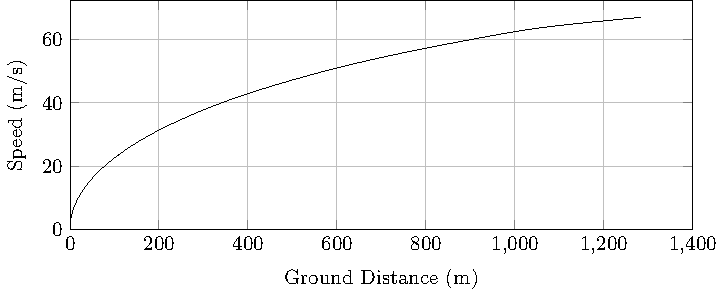
\includegraphics[keepaspectratio, width=1.1\textwidth]{Speed_vs_GroundDistance_AOE}
\caption{Speed v.s. ground distance in AOE condition - ATR-72}
\end{figure}
%
\begin{figure}[H]
\centering
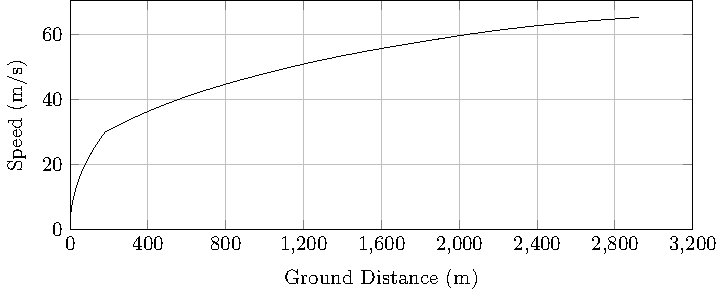
\includegraphics[keepaspectratio, width=1.1\textwidth]{Speed_vs_GroundDistance_OEI}
\caption{Speed v.s. ground distance in OEI condition - ATR-72}
\end{figure}
%
\begin{figure}[H]
\centering
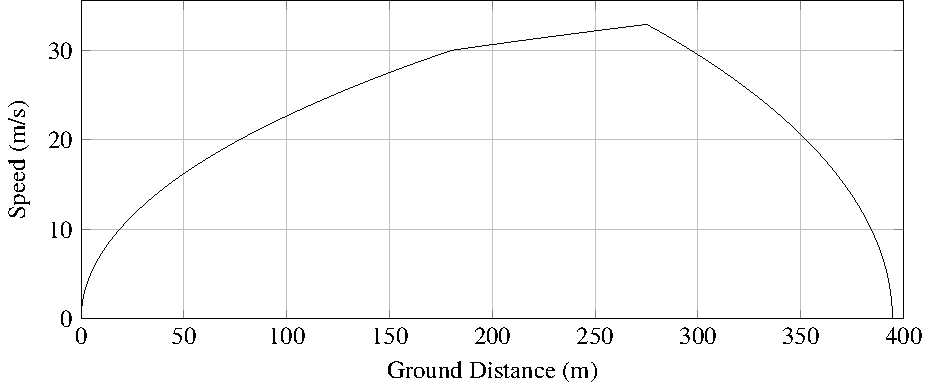
\includegraphics[keepaspectratio, width=1.07\textwidth]{Speed_vs_GroundDistance_ABORTED}
\caption{Speed v.s. ground distance in aborted take-off condition - ATR-72}
\end{figure}
%
\begin{figure}[H]
\centering
%BalancedTakeOffLength
\begin{tikzpicture}

\begin{axis}[
width=\figurewidth,
height=\figureheight,
scaled ticks=false, tick label style={/pgf/number format/fixed},
xmin=0.0,
xmax=1.188,
xlabel={Vfailure/VsTO },
xmajorgrids,
ymin=17.51896136669375,
ymax=2807.8524322653816,
ylabel={Distance (m)},
ymajorgrids,
legend style={at={(1.03,0.5)},anchor=west,draw=black,fill=white,legend cell align=left}
]

\addplot [
color=black,
solid
]
table[row sep=crcr]{
0.03089149187686049	2580.476033742041\\
0.039875596987138974	2580.104775144823\\
0.04885970209741746	2579.3853002216647\\
0.05784380720769594	2579.414843393669\\
0.06682791231797443	2578.83253806873\\
0.0758120174282529	2578.0722733045586\\
0.08479612253853137	2577.9466982926006\\
0.09378022764880985	2577.633718348983\\
0.10276433275908833	2576.2026902544294\\
0.1117484378693668	2575.115930898146\\
0.12073254297964528	2574.6794126376835\\
0.12971664808992378	2574.2272892289348\\
0.13870075320020225	2572.8301153999446\\
0.14768485831048075	2571.855799473663\\
0.15666896342075923	2570.360671897087\\
0.16565306853103773	2569.870571974806\\
0.17463717364131623	2568.395126030281\\
0.1836212787515947	2566.498405013278\\
0.1926053838618732	2565.624120183298\\
0.20158948897215168	2564.371822714379\\
0.21057359408243018	2562.058615241952\\
0.21955769919270868	2560.4117774524884\\
0.22854180430298715	2558.867897919833\\
0.23752590941326565	2557.232243489091\\
0.24651001452354412	2555.682510876605\\
0.2554941196338226	2553.882898298938\\
0.2644782247441011	2551.6470449722756\\
0.2734623298543796	2549.1979773115872\\
0.2824464349646581	2546.85402612102\\
0.2914305400749366	2545.1060964904427\\
0.3004146451852151	2542.9993348770786\\
0.3093987502954936	2540.4114334357473\\
0.31838285540577205	2537.8379880310677\\
0.3273669605160505	2535.3630476925528\\
0.33635106562632905	2532.658779808703\\
0.3453351707366075	2530.079429267451\\
0.354319275846886	2526.8001892445045\\
0.3633033809571645	2524.4775216054013\\
0.372287486067443	2521.372630706008\\
0.38127159117772147	2518.4273603299107\\
0.390255696288	2515.085457941578\\
0.39923980139827847	2511.7747735463463\\
0.40822390650855694	2508.1811660120375\\
0.4172080116188354	2505.518090862105\\
0.42619211672911395	2502.100327736737\\
0.4351762218393924	2498.6969428173743\\
0.4441603269496709	2494.7053077954133\\
0.4531444320599494	2490.843571203638\\
0.4621285371702279	2486.9895856762223\\
0.47111264228050637	2483.226009311492\\
0.4800967473907849	2478.7895781811267\\
0.48908085250106337	2474.950884976647\\
0.49806495761134184	2471.1382773226906\\
0.5070490627216203	2466.9627125741736\\
0.5160331678318988	2462.0489160951784\\
0.5250172729421774	2457.321776166793\\
0.5340013780524558	2453.071994359717\\
0.5429854831627343	2448.318731360877\\
0.5519695882730128	2443.188641545712\\
0.5609536933832913	2438.9070698180367\\
0.5699377984935697	2434.1097898981534\\
0.5789219036038482	2428.6904671206576\\
0.5879060087141268	2423.7714976518764\\
0.5968901138244053	2418.3778805959273\\
0.6058742189346837	2413.0333901086706\\
0.6148583240449622	2407.1201461645187\\
0.6238424291552407	2401.6693843611138\\
0.6328265342655192	2396.1941491453454\\
0.6418106393757976	2390.4805803927347\\
0.6507947444860762	2383.7158703658815\\
0.6597788495963547	2377.9141824696053\\
0.6687629547066332	2372.03620607453\\
0.6777470598169116	2365.5574333641553\\
0.6867311649271901	2359.135842583757\\
0.6957152700374686	2352.635788094017\\
0.7046993751477472	2345.9883509812744\\
0.7136834802580256	2338.715753477014\\
0.7226675853683041	2332.328345944068\\
0.7316516904785826	2325.130293586576\\
0.7406357955888611	2318.12859885101\\
0.7496199006991395	2310.1587206689346\\
0.758604005809418	2303.2452240681905\\
0.7675881109196966	2295.7536307650244\\
0.7765722160299751	2287.2225743531453\\
0.7855563211402535	2279.610561784497\\
0.794540426250532	2271.615917447645\\
0.8035245313608105	2263.8961960565493\\
0.812508636471089	2255.975940563054\\
0.8214927415813674	2246.977311628829\\
0.830476846691646	2238.2199825251255\\
0.8394609518019245	2229.333351135905\\
0.848445056912203	2220.7241580361106\\
0.8574291620224814	2211.1909954457487\\
0.8664132671327599	2202.3295692743195\\
0.8753973722430384	2192.9206989305876\\
0.884381477353317	2183.0648567575226\\
0.8933655824635954	2173.793179083982\\
0.9023496875738739	2164.09562279496\\
0.9113337926841524	2154.3733873265846\\
0.9203178977944309	2143.415760286266\\
0.9293020029047093	2133.5801259046057\\
0.9382861080149878	2123.058569770763\\
0.9472702131252664	2112.4114192600127\\
0.9562543182355449	2101.0734996104857\\
0.9652384233458233	2090.1064976841362\\
0.9742225284561018	2078.8586244910784\\
0.9832066335663803	2067.0100076240406\\
0.9921907386766587	2056.2527391178337\\
1.0011748437869372	2043.2013795744633\\
1.0101589488972156	2031.2226181813026\\
1.019143054007494	2019.231770539278\\
1.0281271591177723	2006.4532893884207\\
1.0371112642280507	1994.2889936986107\\
1.046095369338329	1981.3050573143728\\
1.0550794744486074	1972.0726131694537\\
1.0640635795588858	1966.0476388401612\\
1.0730476846691641	1961.2652752808276\\
1.0820317897794425	1954.6031795553745\\
1.091015894889721	1947.8147172215781\\
1.0999999999999999	1942.7730313876345\\
};

\addplot [
color=black,
densely dashed
]
table[row sep=crcr]{
0.03089149187686049	19.04234931162364\\
0.039875596987138974	22.405206151416166\\
0.04885970209741746	25.940563224683885\\
0.05784380720769594	29.818425168981996\\
0.06682791231797443	33.923033712075394\\
0.0758120174282529	38.33741738333789\\
0.08479612253853137	42.92873780033656\\
0.09378022764880985	47.77318187068427\\
0.10276433275908833	52.936846429000624\\
0.1117484378693668	58.341471713531945\\
0.12073254297964528	63.872401407333285\\
0.12971664808992378	69.75258851097018\\
0.13870075320020225	75.97621467413293\\
0.14768485831048075	82.27373171070337\\
0.15666896342075923	88.77708003116987\\
0.16565306853103773	95.69465975539268\\
0.17463717364131623	102.97558897397161\\
0.1836212787515947	110.40301077608567\\
0.1926053838618732	118.0355229868058\\
0.20158948897215168	125.93564861352391\\
0.21057359408243018	134.22556309066817\\
0.21955769919270868	142.93563199782056\\
0.22854180430298715	151.6604194913029\\
0.23752590941326565	160.50901180984664\\
0.24651001452354412	169.78156369888313\\
0.2554941196338226	179.19494935785542\\
0.2644782247441011	189.4031072910226\\
0.2734623298543796	199.43234003340365\\
0.2824464349646581	209.507431936077\\
0.2914305400749366	220.43987826403594\\
0.3004146451852151	231.37346365839778\\
0.3093987502954936	242.32316620695173\\
0.31838285540577205	253.8292738199441\\
0.3273669605160505	265.76940785274724\\
0.33635106562632905	277.7601027892989\\
0.3453351707366075	290.10944424556874\\
0.354319275846886	302.5450145578369\\
0.3633033809571645	315.5196426463946\\
0.372287486067443	329.14046262059026\\
0.38127159117772147	342.34942025268595\\
0.390255696288	355.880005108786\\
0.39923980139827847	370.3405177565718\\
0.40822390650855694	384.47262398543717\\
0.4172080116188354	398.9883918457051\\
0.42619211672911395	414.2158990735667\\
0.4351762218393924	429.6487709906082\\
0.4441603269496709	444.76364261501817\\
0.4531444320599494	461.15646030751225\\
0.4621285371702279	476.79162050111756\\
0.47111264228050637	493.60877548912015\\
0.4800967473907849	510.50224015310687\\
0.48908085250106337	527.3477961827114\\
0.49806495761134184	544.9346460378686\\
0.5070490627216203	562.64266440759\\
0.5160331678318988	581.1273504208011\\
0.5250172729421774	598.9369065675969\\
0.5340013780524558	617.3913020729362\\
0.5429854831627343	637.4360853936723\\
0.5519695882730128	656.5665982797905\\
0.5609536933832913	675.4455763490587\\
0.5699377984935697	696.2938029480754\\
0.5789219036038482	716.6080885961301\\
0.5879060087141268	736.976909193753\\
0.5968901138244053	757.7356980629954\\
0.6058742189346837	779.4034626917157\\
0.6148583240449622	801.7581844753722\\
0.6238424291552407	824.000081848583\\
0.6328265342655192	846.8407428941957\\
0.6418106393757976	869.2605371711818\\
0.6507947444860762	892.5901715779382\\
0.6597788495963547	915.0644043583086\\
0.6687629547066332	939.7085136029243\\
0.6777470598169116	963.0247644893263\\
0.6867311649271901	988.2515260472144\\
0.6957152700374686	1013.4758924106811\\
0.7046993751477472	1039.0408112669238\\
0.7136834802580256	1063.9534479741264\\
0.7226675853683041	1091.473220985582\\
0.7316516904785826	1117.5139579472057\\
0.7406357955888611	1144.7466210499524\\
0.7496199006991395	1171.7523890250673\\
0.758604005809418	1199.5114391331276\\
0.7675881109196966	1227.2958441027436\\
0.7765722160299751	1256.7989656703849\\
0.7855563211402535	1284.7755595998324\\
0.794540426250532	1315.5489724982713\\
0.8035245313608105	1343.9577352309834\\
0.812508636471089	1374.625011522061\\
0.8214927415813674	1406.2179516186484\\
0.830476846691646	1436.2174472860238\\
0.8394609518019245	1467.4214959429614\\
0.848445056912203	1499.74374189144\\
0.8574291620224814	1531.7856298596153\\
0.8664132671327599	1565.4170323455492\\
0.8753973722430384	1599.1708289699077\\
0.884381477353317	1633.3848032242645\\
0.8933655824635954	1668.0049440388734\\
0.9023496875738739	1701.278899933815\\
0.9113337926841524	1736.652548884219\\
0.9203178977944309	1772.2503405131451\\
0.9293020029047093	1809.2961976664014\\
0.9382861080149878	1844.7531971762573\\
0.9472702131252664	1882.2765872014102\\
0.9562543182355449	1921.8621719435223\\
0.9652384233458233	1960.675813548297\\
0.9742225284561018	1998.2253783662372\\
0.9832066335663803	2037.355434289851\\
0.9921907386766587	2077.7288622888336\\
1.0011748437869372	2116.820873082638\\
1.0101589488972156	2158.196417879045\\
1.019143054007494	2200.9055983839\\
1.0281271591177723	2243.1058560310767\\
1.0371112642280507	2283.1675876696045\\
1.046095369338329	2327.8517281335953\\
1.0550794744486074	2371.036972543575\\
1.0640635795588858	2417.377606686301\\
1.0730476846691641	2459.705866665855\\
1.0820317897794425	2504.8956869791054\\
1.091015894889721	2553.7378972992146\\
1.0999999999999999	2599.8633632086867\\
};
\end{axis}
\end{tikzpicture}%

\caption{Balanced take-off length chart - ATR-72}
\end{figure}
%